% Tipo de documento:
\documentclass[12pt,a4paper,onecolumn,oneside]{report}
\newcommand{\mychapter}[2]{
	\setcounter{chapter}{#1}
	\setcounter{section}{0}
	\chapter*{#2}
	\addcontentsline{toc}{chapter}{#2}
}

% Opcional: Tamaño personalizado para los márgenes:
\usepackage[a4paper, top=3cm, bottom=3cm, left=3cm, right=3cm]{geometry}
\usepackage{pifont}
\usepackage{float}
\usepackage{array}
\usepackage{amsmath}
\usepackage{lscape}
\usepackage{longtable}
\newcommand{\tabtitle}[1]{\cellcolor{CSGreen}\color{white}\textbf{#1}\rule{0pt}{20pt}}
\newcommand{\ltt}[1]{\cellcolor{CSGreen}\color{white}\textbf{#1}\rule{0pt}{8pt}}
\newcommand{\rtabtitle}[1]{\cellcolor{CSRed}\color{white}\textbf{#1}\rule{0pt}{20pt}}
\usepackage{multirow}
\usepackage[utf8]{inputenc} % Codificación UTF-8.
\usepackage[T1]{fontenc}    % Para usar caracteres con tilde.
\usepackage[spanish,es-tabla]{babel} % Escritura en castellano.
\usepackage{eurosym}  % Para el símbolo del EURO (€).
\usepackage{graphicx} % Paquete de imágenes, para introducir figuras.
\DeclareGraphicsExtensions{.pdf,.png,.jpg}
\usepackage[usenames,dvipsnames]{color} % Texto en colores.
\usepackage[table, RGB, usenames,dvipsnames]{xcolor}   % Extra colors.
\definecolor{codegreen}{rgb}{0,0.6,0}
\definecolor{codegray}{rgb}{0.5,0.5,0.5}
\definecolor{codepurple}{rgb}{0.58,0,0.82}
\definecolor{backcolour}{rgb}{0.95,0.95,0.92}
\definecolor{lesslightblue}{rgb}{0.7,0.7,1.0}
\usepackage{listings}
\lstdefinestyle{mystyle}{
    backgroundcolor=\color{backcolour},
    commentstyle=\color{codegreen},
    keywordstyle=\color{magenta},
    stringstyle=\color{codepurple},
    basicstyle=\ttfamily\footnotesize,
    breakatwhitespace=false,
    breaklines=true,
    captionpos=b,
    keepspaces=true,
    showspaces=false,
    showstringspaces=false,
    showtabs=false,
    tabsize=2
}

\lstdefinelanguage{shell}
{
  backgroundcolor=\color{black},
  rulecolor=\color{codegray},
  basicstyle=\footnotesize\ttfamily\color{white},
  morecomment=[l]{\#},
  commentstyle=\footnotesize\ttfamily\color{lesslightblue}
}

\lstset{style=mystyle}

\usepackage{enumitem} % Para personalizar listas de items.

\renewcommand{\lstlistingname}{Script}
% \usepackage{url}      % Para escritura de URLs.
\usepackage[hyphens]{url}
\usepackage{subcaption} % Para montar grid de imágenes
\usepackage[breaklinks]{hyperref} % Hiperreferencias.
\usepackage{amsmath,amssymb} % Para los símbolos matemáticos.
\usepackage{cite}     % Para las citas de referencias (crea el superíndice).
\usepackage{listings} % Para coloreado de código fuente.
\usepackage{verbatim} % Para textos tipo consola y otros formatos.
\usepackage{fancyvrb} % Más opciones de verbatim.
\usepackage{parskip}  % OPCIONAL: Separa los párrafos con una línea en blanco.
\setlength{\parindent}{15pt} % Sangría de párrafos estándar (15 puntos). Necesario incluirla si se usa el paquete 'parskip'.
\usepackage[export]{adjustbox}
\usepackage{caption}  % Para personalizar los pies de foto.

% Opciones del paquete caption para los pies de imágenes y tablas:
\captionsetup{figurename=Figura, tablename=Tabla, labelsep=colon, labelfont=bf, font=small, justification=centering}

% Para el control de líneas viudas y huérfanas (líneas sueltas en páginas nuevas):
\usepackage[all]{nowidow}

\usepackage[nottoc]{tocbibind}    % Incluye el apartado "Referencias" en el índice.
%\def\spanishrefname{Bibliografía} % Para que ponga "Bibliografía" en lugar de "Referencias". SÓLO se aplica a formato "article". En "report" ya pone "Bibliografía".

\usepackage{fancyhdr}

\setlength{\unitlength}{1 cm} % Unidad de trabajo de medidas.

\renewcommand*{\baselinestretch}{1.25} % Altura del INTERLINEADO.
\renewcommand{\shorthandsspanish}{}    % Para que corte las palabras según el castellano.
\usepackage{makecell}

\usepackage[table, RGB, usenames,dvipsnames]{xcolor}   % Extra colors.
\usepackage{booktabs} % tablas con mejor estilo (toprule/midrule/bottomrule)
\usepackage{siunitx}  % formato numérico en tablas
\sisetup{group-separator = {,}, detect-all, round-mode=places, round-precision=2}

% Propiedades para el PDF generado (METADATOS):
\newcommand{\authorNames}{Aitor García Blanco}
\newcommand{\pdftitle}{Detección de células defectuosas en imágenes médicas}
\hypersetup{
  pdftitle={\pdftitle},% Título
  pdfauthor={\authorNames},% Autor
  pdfsubject={\pdftitle \ - \authorNames},% Asunto
% pdfkeywords={Opcional: algunas palabras clave}%
}

% Para la representación de código fuente:
% Para BASH:
\lstset{
	language=bash,
	basicstyle=\scriptsize,
	frame=single,
	numbers=left,
	numberstyle=\scriptsize,
	stepnumber=1,
	numbersep=9pt,
	backgroundcolor=\color{White},
	showspaces=false,
	showstringspaces=false,
	showtabs=false,
	tabsize=4,
	captionpos=b,
	breaklines=true,
	keywordstyle=\color{blue}\bfseries,
	%identifierstyle=\color{green}\bfseries,
	stringstyle=\color{orange}\bfseries,
	commentstyle=\color{gray}\bfseries
}
% Para C++:
%\lstset{
%	language=C++,
%	frame=single,
%	keywordstyle=\color{Green}\bfseries,
%	identifierstyle=\color{BlueViolet},
%	stringstyle=\color{Red},
%	commentstyle=\color{MidnightBlue}
%}

\usepackage{fancyhdr} % Para el tamaño y estilo de los encabezados.

\fancypagestyle{headings}{% Redefine el estilo "headings".
	\fancyhf{} % Clear all header and footer fields.
	\lhead{\small \it Máster Universitario en Robótica e Inteligencia Artificial} 
	\rhead{\small \it Página \thepage}      % Nº de página a la derecha. Tamaño "small".
	\renewcommand{\headrulewidth}{1pt}
}

% Ajustes para división manual de palabras:
\hyphenation{Python} % Impide que la palabra Python sea dividida al acabar una línea.

\usepackage{titlesec}
\titleformat{\chapter}[hang]
  {\normalfont\huge\bfseries}
  {\thechapter.}{1em}{}

\titlespacing*{\chapter}{0pt}{0pt}{1em}
%%%%%%%%%%%%%%%%%%%%%%%%%%%%%%%%%%%%%%%%%%%%%%%%%%%%%%%%%%%%%%%%%%%%%%%%%%%%%%%%%%%%%%%%%%%%%%%%%%%%%%%%%%%%%%%%%%%%%
%%%%%%%%%%%%%%%%%%%%%%%%%%%%%%%%%%%%%%%%%% INICIO DEL DOCUMENTO: %%%%%%%%%%%%%%%%%%%%%%%%%%%%%%%%%%%%%%%%%%%%%%%%%%%%
%%%%%%%%%%%%%%%%%%%%%%%%%%%%%%%%%%%%%%%%%%%%%%%%%%%%%%%%%%%%%%%%%%%%%%%%%%%%%%%%%%%%%%%%%%%%%%%%%%%%%%%%%%%%%%%%%%%%%
\renewcommand{\chaptername}{}
\begin{document}

% Página de TÍTULO (portada):
\begin{titlepage}

\begin{picture}(0,0)
\put(-1,-2){
\includegraphics[height=3cm]{figuras/logos/logo_master.png}}
\end{picture}

\begin{picture}(0,0)
\put(10,-1.5){
\includegraphics[height=3cm]{figuras/logos/logo_ule.png}}
\end{picture}

\begin{center}
\vspace{3cm}
\textbf{{\Large \bf Departamento de Ingenierías}}\\[0.5cm]
\textbf{{\Large \bf Mecánica, Informática y Aeroespacial}}\\[2cm]
{\Large \bf MÁSTER UNIVERSITARIO EN ROBÓTICA E \\ INTELIGENCIA ARTIFICIAL}\\[2.5cm]
{\Large Trabajo de Fin de Máster}\\[2.0cm]
{\Large \textbf{Detección de células defectuosas sobre un conjunto de imágenes médicas}\\[0.8cm]} %[0.1cm]} 
%{\Large \textbf{Sistema cognitivo para ROS 2\\[2cm]}}
{\Large \textbf{Detection of Defective Cells in a Set of Medical Images}\\[1.5cm]} %[0.1cm]} 
%{\Large \textbf{Cognitive System for ROS 2\\[2cm]}}
\end{center}

\begin{flushright}
{\bf Autor: Aitor García Blanco}\\[0.3cm]
{\bf Tutor: Laura Fernández Robles}\\[0.3cm]
%{\bf Co-Tutor: }\\[0.3cm]
%{\bf ~}\\[0.5cm]
\end{flushright}


\end{titlepage}

% Página de FIRMAS:
\newpage

\thispagestyle{empty} % para que no se numere esta página.

\begin{center}
%{\huge (Septiembre, 2025)}
\end{center}

\setlength{\LTleft}{-1.25cm}      % Desplaza la tabla 1cm a la izquierda
\setlength{\LTright}{0pt}      % Mantiene el margen derecho normal

\begin{longtable}{|l|l|}
	\cline{1-2}
	\multicolumn{2}{|c|}{}	\\
	\multicolumn{2}{|c|}{\textbf{UNIVERSIDAD DE LEÓN}}	\\
	\multicolumn{2}{|c|}{\textbf{Departamento de Ingenierías Mecánica, Informática y Aeroespacial}}	\\ 
	\multicolumn{2}{|c|}{\textbf{MÁSTER UNIVERSITARIO EN ROBÓTICA E INTELIGENCIA ARTIFICIAL}}	\\
	\multicolumn{2}{|c|}{\textbf{Trabajo de Fin de Máster}}	\\ 
	\multicolumn{2}{|c|}{}	\\ \hline
	\multicolumn{2}{|l|}{\textbf{ALUMNO}: Aitor García Blanco}	\\ \hline
	\multicolumn{2}{|l|}{\textbf{TUTOR}: Laura Fernández Robles}	\\ \hline
	\multicolumn{2}{|p{17cm}|}{\textbf{TÍTULO}: Sistema automatizado para la detección de células redondas en imágenes médicas mediante aprendizaje profundo} \\ \hline
	\multicolumn{2}{|p{17cm}|}{\textbf{TITLE}: Automated detection of round cells in medical images using deep learning} \\ \hline
	\multicolumn{2}{|l|}{\textbf{CONVOCATORIA}: Septiembre, 2025}		\\ \hline
	\multicolumn{2}{|p{17cm}|}{\textbf{RESUMEN}: Con el objetivo de optimizar el análisis seminal, un proceso clave en la medicina reproductiva, 
	se aborda el diseño, desarrollo y validación de un sistema automatizado para la detección de células redondas en imágenes de muestras de semen 
	humano sin procesar, mediante técnicas de aprendizaje profundo y visión por computador.
	
	La metodología se centra en la consolidación de un dataset validado por expertos. Posteriormente, se aborda el entrenamiento y la optimización de 
	diversas arquitecturas del modelo YOLO (de la v8 a la v12), incluyendo la creación de un modelo con arquitectura personalizada y otro ensamblado (\textit{ensemble})
	que fusiona las fortalezas de YOLOv10s y YOLOv12s. Para maximizar su rendimiento se aplican técnicas de ajuste fino (\textit{fine-tuning}) y aumento de datos 
	(\textit{data augmentation}), junto con una sistemática optimización de hiperparámetros con Optuna y una evaluación mediante validación cruzada. 
	Los resultados demuestran que el mejor modelo para abordar esta problemática es el YOLOv12s, que supera significativamente el rendimiento de 
	sistemas anteriores.
	
	El proyecto culmina con el desarrollo de una herramienta web interactiva que traduce los diferentes modelos de inteligenia artificial 
	en una solución práctica y funcional, que facilita la validación de resultados por parte del especialitas y sienta las bases para su futura integración en entornos clínicos, potenciando así 
	la transformación digital en el campo de la andrología.} \\ \hline

	\multicolumn{2}{|p{17cm}|}{\textbf{Palabras clave}: detección de objetos, células redondas, 
	análisis de semen, inteligencia artificial, aprendizaje profundo, visión por computador, YOLO}	\\
	\hline

	\multicolumn{2}{|p{17cm}|}{\textbf{ABSTRACT}: To optimize semen analysis, a key process in reproductive medicine, this project addresses the design, 
	development, and validation of an automated system for detecting round cells in images of unprocessed human semen samples using deep learning and 
	computer vision techniques.

	The methodology focused on the consolidation of an expert-validated dataset. Subsequently, various YOLO model architectures (from v8 to v12) were trained 
	and optimized, including the creation of a custom architecture model and an ensemble model that combines the strengths of YOLOv10s and YOLOv12s. 
	To maximize performance, techniques such as fine-tuning and data augmentation were applied, along with systematic hyperparameter optimization using Optuna 
	and evaluation through cross-validation. The results demonstrate that the best model to address this problem is YOLOv12s, which significantly outperforms 
	previous systems.

	The project culminates in the development of an interactive web tool that translates the artificial intelligence models into a practical and 
	functional solution. This tool facilitates the validation of results by specialists and lays the groundwork for its future integration into 
	clinical environments, thereby advancing the digital transformation in the field of andrology.} \\ 
	\hline
	\multicolumn{2}{|p{17cm}|}{\textbf{Keywords}: object detection, round cells, 
	semen analysis, artificial intelligence, deep learning, computer vision, YOLO}	\\ 
	\hline
\end{longtable}

\newpage
\pagestyle{plain}

\renewcommand{\thepage}{\roman{page}}
\setcounter{page}{1} % Esta página es la 1.

% Página con el ÍNDICE GENERAL
\renewcommand{\contentsname}{Índice}
\tableofcontents

% Página con el ÍNDICE DE FIGURAS
\listoffigures

% Página con el ÍNDICE DE TABLAS
\listoftables

%%%%%%%%%%%%%%%%%%%%%%%%%%%%%%%%%%%%%%%%%%%%%%%%%%%%%%%%%%%%%%%%%%%%%%%%%%%%%%%%%%%%%%%%%%%%%%%%%%%%%%%%%%%%%%%%%%%%%
%%%%                                            Glosario de Términos                                             %%%%
%%%%%%%%%%%%%%%%%%%%%%%%%%%%%%%%%%%%%%%%%%%%%%%%%%%%%%%%%%%%%%%%%%%%%%%%%%%%%%%%%%%%%%%%%%%%%%%%%%%%%%%%%%%%%%%%%%%%%
% Página con el GLOSARIO:
\mychapter{0}{Glosario de términos}
\label{chap:glosario}
% A partir de aquí ya se incluye el encabezado en las páginas:
\pagestyle{headings}

% Al ser un capítulo sin número, hay que indicarle qué título añadir al encabezado de la página:
\markboth{GLOSARIO}{} 

\begin{description}
  \item[\textit{Bounding box}:] Rectángulo que delimita la posición y tamaño de un objeto en una imagen.
  \item[\textit{Dataset}:] Conjunto de datos estructurados, utilizado para entrenar, validar o evaluar modelos de inteligencia artificial.
  \item[IoU (\textit{Intersection over Union}):] Área de unión entre dos \textit{bounding boxes} (anotación y predicción).
  \item[Métricas:] Indicadores cuantitativos para la evaluación de los modelos de inteligencia artificial.
  \item[Experto:] Persona con conocimientos especializados en un dominio específico (como biólogos, biotecnólogos, patólogos, etc.).
  \item[Detección de objetos:] Tarea de localizar y clasificar instancias de objetos en imágenes mediante \textit{bounding boxes} y etiquetas. 
  \item[NMS (\textit{Non-Maximum Suppression}):] Algoritmo para eliminar las detecciones redundantes, manteniendo la caja con mayor confianza entre las solapadas.
  \item[Aprendizaje profundo o \textit{deep learning}:] Área del aprendizaje automático que emplea redes neuronales profundas para aprender representaciones y resolver tareas complejas.
  \item[Aprendizaje por transferencia (\textit{Transfer Learning}):] Estrategia de aprendizaje automático que consiste en reutilizar un modelo preentrenado en una tarea para aplicarlo como punto de partida en una segunda 
  tarea distinta pero relacionada. En lugar de entrenar un modelo desde cero, se aprovecha el "conocimiento" (pesos y características) ya adquirido.
  \item[Ajuste fino (\textit{Fine-Tuning}):] Técnica específica del aprendizaje por transferencia. Consiste en tomar un modelo preentrenado y continuar su entrenamiento sobre un nuevo conjunto de datos más específico. 
  Durante este proceso, los pesos del modelo se "ajustan" o refinan, generalmente con una tasa de aprendizaje baja, para adaptar las características aprendidas previamente a las demandas de la nueva tarea.
  \item[\textit{Framework}:] Conjunto estructurado de herramientas, librerías y convenciones que facilita y agiliza el desarrollo de aplicaciones o sistemas.
  % \item[\textit{Ensemble}]: Técnica para la unificación de predicciones de diferentes modelos.
  % \item[\textit{Cross Validatio}]: Técnica estadística para la evaluación de modelos, que se fundamenta en dividir el \textit{dataset} en multiples pliegues (\textit{folds}) para entrenar y validar el modelo de forma iteractiva.
  % \item[\textit{Data augmentation}]: Conjunto de transformaciones sobre los datos como rotaciones, traslaciones, adición de ruido, entro otros, con el objetivo de aumentar la diversidad del dattaset y mejorar la generalización del modelo.
  % \item[Optuna]: Biblioteca de Python para la optimización de hiperparámetros, permitiendo encontrar las mejores configuraciones de estos. 
  \item[\textit{Streamlit}:] \textit{Framework} de Python para crear aplicaciones web interactivas orientadas a la ciencia de datos y \textit{Machine Learning}.
  \item[Monolítica:] Arquitectura de software en la que la aplicación se despliega y ejecuta en un mismo proceso.     
  \item[\textit{LabelImg}:] Herramienta gráfica de código abierto para la anotación de imágenes con \textit{bounding boxes}.
  \item[\textit{Widget}:] Elemento de una interfaz interactiva que permite al usuario controlar el comportamiento de una aplicación.
  \item[\textit{Ground truth}:] Hace alusión a las anotaciones correctas que describen las \textit{bounding boxes} de las imágenes.
  \item[\textit{Checkbox}:] Es un \textit{widget} que permite al usuario activar o desactivar una opción (booleano).  
  \item[\textit{Linter}:] Herramienta que analiza automáticamente el código fuente para detectar errores de sintaxis u otros posibles fallos antes de ejecutar el programa. 
  \item[Células redondas:] Según la OMS \cite{OMS}, toda célula no espermática que se encuentra en el eyaculado. Agrupa principalmente dos tipos: células germinales inmaduras y leucocitos.
  \item[Células germinales inmaduras:] Células precursoras de los espermatozoides que no han completado su desarrollo.
  \item[Leucocitos:] Glóbulos blancos, principalmente neutrófilos.  
  \item[Espermograma:] Consiste en analizar los espermatozoides de un hombre o un animal para evaluar la fertilidad y detectar posibles anomalías. 
  \item[Espermatogénesis:] Proceso biológico de formación y producción de espermatozoides.
  \item[Andrología:] Área de la medicina que se centra en el estudio e investigación de cualquier aspecto relacionado con la función sexual y reproducción masculina (Por ejemplo: infertilidad masculina).  
  \item[Anillos de Newton:] Interferencia de la luz cuyo resultado es un patrón de anillos muy característico.
  \item[\textit{Overfitting}:] Proceso en el que un modelo de aprendizaje automático aprende demasiado bien los datos de entrenamiento, perdiendo capacidad de generalización y obteniendo peores resultados en las pruebas de evaluación.
  \item[TP (Verdaderos Positivos):] Células redondas correctamente detectadas por el modelo. El algoritmo identifica correctamente una célula redonda, que efectivamente, existe en la muestra de semen.
  \item[FP (Falsos Positivos):] Detecciones incorrectas. Donde el modelo identifica una célula redonda que en realidad no existe o corresponde a otro elemento (como un espermatozoide sin cola o un artefacto visual).
  \item[TN (Verdaderos Negativos):] Regiones de la imagen correctamente no marcadas como células redondas. Representan áreas donde el modelo no detecta ninguna célula.
  \item[FN (Falsos Negativos):] Células redondas presentes en la muestra que el modelo no detecta.
  \item[GVIS:] Group for Vision and Intelligent Systems de la Universidad de León.  
  \item[Inferencia:] Proceso de utilizar un modelo entrenado para hacer predicciones sobre imágenes nuevas o no vistas previamente.
  \item[PASCAL VOC:] Formato de anotación de imágenes (\textit{Pattern Analysis, Statistical Modelling and Computational Learning Visual Object Classes}). 
  Es un estándar para la anotación de objetos en imágenes mediante \textit{bounding boxes} rectangulares, almacenadas en archivos XML. Cada anotación incluye las coordenadas del 
  rectángulo (xmin, ymin, xmax, ymax) y la clase del objeto.
  \item[COCO:] Formato de anotación (\textit{Common Objects in Context}) que proporciona un estándar más completo para la detección de objetos, segmentación y etiquetado de imágenes. Utiliza archivos JSON para 
  almacenar información sobre imágenes, categorías y anotaciones.
\end{description} 

%%%%%%%%%%%%%%%%%%%%%%%%%%%%%%%%%%%%%%%%%%%%%%%%%%%%%%%%%%%%%%%%%%%%%%%%%%%%%%%%%%%%%%%%%%%%%%%%%%%%%%%%%%%%%%%%%%%%%
%%%%                                           Inicio de los CAPÍTULOS                                           %%%%
%%%%%%%%%%%%%%%%%%%%%%%%%%%%%%%%%%%%%%%%%%%%%%%%%%%%%%%%%%%%%%%%%%%%%%%%%%%%%%%%%%%%%%%%%%%%%%%%%%%%%%%%%%%%%%%%%%%%%
\newpage
\renewcommand{\thepage}{\arabic{page}}
\setcounter{page}{1} % Esta página es la 1.

\chapter{Introducción y objetivos} %%%%%%%%%%%%%%%%%%%%%%%%%%%%%%%%%%%%%%%%%%%%%%%%%%%%%%%
\label{Introducción y objetivos}
\section{Introducción}
\label{sec:Introducción}

El presente Trabajo de Fin de Máster, desarrollado en colaboración con la empresa Microptic S.L \cite{microptic}, compañía de Hamilton Thorne \cite{HamiltonThorneWeb}, 
parte del desarrollo de una Prueba de Concepto (\textit{Proof of Concept}) desarrollada en el marco europeo DIGIS3 \cite{digis3} para la detección de células redondas en imágenes médicas 
mediante inteligencia artificial.

El objetivo de esta solución es la identificación automatizada de células redondas en imágenes de muestras de semen humano. Esta capacidad es de 
gran interés para Microptic \cite{microptic}, ya que optimiza los tiempos de análisis de los expertos y enriquece el estudio de las muestras espermáticas, 
mejorando la caracterización de parámetros clave tanto en el ámbito de la reproducción asistida humana como en la investigación y producción animal. 

La metodología se ha centrado, en primer lugar, en la consolidación de un conjunto de datos de alta calidad. Para ello, se procesó y validó el \textit{feedback} 
proporcionado por los expertos de Microptic \cite{microptic}, refinando el etiquetado de las imágenes que constituyen la base para la evaluación de los modelos.

Posteriormente, aplicando técnicas de aprendizaje profundo (\textit{Deep Learning}) y visión por computador, se adaptaron y reentrenaron varias versiones 
del modelo de detección de objetos en tiempo real YOLO \cite{ultralytics_models}, un modelo personalizado y un \textit{ensemble} de modelos. El propósito fue especializar su capacidad, pasando de la detección de objetos 
cotidianos a la identificación precisa de células redondas. Finalmente, el modelo fue entrenado y evaluado para validar su rendimiento, eficacia y viabilidad.

Este trabajo incluye la creación de una interfaz digital que permite
al proyecto trascender la investigación académica para dar continuidad a la misión de DIGIS3 \cite{digis3}: "impulsar la digitalización de las empresas a través 
de soluciones tecnológicas avanzadas". La herramienta web desarrollada actúa como un catalizador de la transformación digital para Microptic \cite{microptic}, traduciendo 
un complejo modelo de inteligencia artificial en una solución práctica que potencia sus capacidades de análisis y establece un precedente para futuras innovaciones.

\section{Objetivos}
\label{sec:Objetivos}

Este Trabajo de Fin de Máster tiene como objetivo principal diseñar, desarrollar y validar de un sistema inteligente para la detección automatizada de células redondas en imágenes médicas de muestras de semen humano
mediante el empleo de técnicas de visión por computador y aprendizaje profundo. 
Se de muestra así, la integración de competencias técnicas avanzadas en inteligencia artificial, procesamiento de imágenes y desarrollo de \textit{software}, entre otras habilidades transversales. 

Con este proyecto, se abordan los siguientes objetivos específicos: 

\begin{itemize}
  \item Investigar y estudiar casuísticas análogas en la detección de células en conjuntos de imágenes médicas y establecer un estado del arte de la cuestión.
  \item Realizar un preprocesamiento y anotación de los conjuntos de imágenes médicas.
  \item Implementar, entrenar y validar diferentes modelos u arquitecturas de modelos, comparar su rendimiento y optimizar hiperparámetros.
  \item Evaluar cuantitativa y cualitativamente los modelos mediante métricas estándar y la observación visual de los resultados.
  \item Desarrollar una herramienta web interactiva para visualización, inferencia y exportación de resultados que facilite la validación por parte de expertos biomédicos.
  \item Garantizar la reproducibilidad y cumplimiento ético y legislativo.
  \item Documentar exhaustivamente el proyecto.
\end{itemize}


\chapter{Antecedentes} %%%%%%%%%%%%%%%%%%%%%%%%%%%%%%%%%%%%%%%%%%%%%%%%%%%%%%%
\label{Antecedentes}

En este capítulo se expone el problema abordado en este trabajo, sus antecedentes, hipótesis y motivaciones. 
Asimismo, se revisa la literatura existente para situar el estado del arte y justificar la necesidad de la investigación realizada.

\section{Contexto y motivación}
\label{sec:Contexto y motivación}

El análisis de muestras de semen es un pilar fundamental en el campo de la medicina reproductiva. Su relevancia abarca desde el diagnóstico 
de la infertilidad en parejas y técnicas de reproducción asistida en humanos, hasta la investigación y producción en el sector ganadero. Tradicionalmente,
este análisis se ha centrado en la motilidad, concentración y morfología de los espermatozoides.

Sin embargo, un análisis seminal requiere la evaluación de otros componentes celulares, entre los que destacan las células redondas. 
Estas constituyen un indicador de diagnóstico crucial, ya que abarcan linfocitos, células plasmáticas, macrófagos, mastocitos y células tumorales redondas, cuya presencia puede ser signo de infecciones o inflamaciones 
del tracto genital, como células germinales inmaduras, que pueden indicar una alteración en el proceso de espermatogénesis \cite{HamiltonThorneRoundCells}.

El método estándar para la identificación y conteo de células redondas depende de la agudeza visual de un experto a través de un microscopio; esto lo convierte en
un proceso subjetivo, lento, laborioso y cansado para el observador. Estas limitaciones motivan la necesidad 
de desarrollar alternativas mediante herramientas automatizadas que permitan obtener resultados más rápidos, objetivos y reproducibles, optimizando el espermograma.

El auge de la inteligencia artificial, y en particular las técnicas de visión por computador basadas en aprendizaje profundo, están protagonizando una revolución dentro del mundo de la medicina.
La capacidad de las redes neuronales en la detección de patrones complejos ha demostrado ser una herramienta de apoyo en diversas especialidades como son: análisis de imágenes radiológicas o análisis de lesiones cutáneas en dermatología, entre otras.
En \textit{computer vision}, modelos de detección de objetos como YOLO (\textit{You Only Look Once}) \cite{ultralytics_models} han demostrado un equilibrio entre precisión y velocidad de inferencia. Estos algoritmos son capaces 
de procesar imágenes y localizar múltiples objetos de interés en milisegundos, siendo idóneo en este tipo de trabajos clínicos.

Atendiendo a estas necesidades y casuísticas, por parte de una empresa líder en el análisis espermático, surge la necesidad de integrar estos sistemas inteligentes para la detección de células redondas a la que dio solución el grupo GVIS de la 
Universidad de León mediante una \textit{Proff of Concept} (PoC) \cite{HamiltonThorneRoundCells}. Demostrando así, la capacidad de estas tecnologías en este tipo de tareas complejas.

Aprovechando este hito, surge la motivación de definir una nueva prueba de concepto (PoC) integrada en un entorno digital, que permita igualar o superar con menos recursos, la anterior PoC. Esto se aborda a través de diferentes vías:

\begin{itemize}
  \item Explorar diferentes arquitecturas de YOLO \cite{ultralytics_models}, desde modelos oficiales hasta prototipos más recientes que emplean capas de atención. 
  \item Diseñar un modelo personalizado para competir con los modelos existentes.
  \item Optimización y mejora de la detección: buscar la configuración óptima que maximice diferentes métricas y abordar la detección de artefactos visuales que fueron identificados como una limitación en la PoC previa. 
  \item Desarrollar una herramienta web interactiva que no solo sirva para evaluar imágenes sino que además, dé soporte a expertos.
\end{itemize}

\section{Estado del arte e hipótesis}
\label{sec:Estado del arte e hipótesis}

En esta sección se analiza el panorama tecnológico que sirve como fundamento para este proyecto. Se parte de las tecnologías de inteligencia artificial que tienen relevancia en el campo de la medicina como es la 
visión por computador, se abordan los modelos de detección de objetos utilizados y se revisan las diferentes técnicas de optimización. Finalmente, se realiza un breve estudio sobre la literatura actual 
en este campo y se define la hipótesis de trabajo.

\subsection{Visión por computador y modelos de detección de objetos}
\label{sec:Arquitecturas}

La inteligencia artificial está en auge y algunos de los campos en los que está tomando protagonismo son el aprendizaje profundo y la visión por computador. 
Estos son los campos en los que se fundamenta esta PoC. La visión por computador está revolucionando el análisis de imágenes dadas las capacidades de estos 
sistemas de interpretar datos visuales en tareas como la clasificación, segmentación semántica o la detección de objetos.
La detección de objetos se fundamenta en aprendizaje profundo, mediante el uso de redes neuronales. Los algoritmos pueden identificar patrones complejos en las imágenes con una precisión 
que no deja de sorprender. 

Dentro de este campo, la detección de objetos tiene como objetivo localizar espacialmente (mediante \textit{bounding boxes}) y clasificar cada una de las múltiples instancias de un objeto de interés dentro de una misma imagen.
Esta tarea es crucial para este proyecto, pues va a permitir detectar y cuantizar las células redondas en una imagen de esperma humano.

La familia de modelos de YOLO \cite{ultralytics_models} se ha consolidado como un referente para tareas de detección, permitiendo un equilibrio entre precisión y velocidad.
Dentro de las 12 arquitecturas de YOLO \cite{ultralytics_models}, se emplean las siguientes:

\begin{itemize}
  \item \textbf{YOLOv8:} Adopta un diseño eficiente y sin anclajes (\textit{anchor-free}). Su arquitectura utiliza una versión refinada de módulos basados en \textit{Cross-Stage Partial} CSP y una cabeza desacoplada que separa las tareas de clasificación y regresión, logrando un buen equilibrio entre velocidad y precisión \cite{defyolos} (\autoref{fig:Yolov8_v9_v10_arquitectures}).
  \item \textbf{YOLOv9:} Introduce la Información de Gradiente Programable (PGI) y la Red de Agregación de Capas Generalizada y Eficiente (GELAN). Estas innovaciones ayudan a mantener gradientes robustos a través de la red, mejorando la convergencia y la capacidad para detectar objetos pequeños al evitar la pérdida de información \cite{defyolos} (\autoref{fig:Yolov8_v9_v10_arquitectures}).
  \item \textbf{YOLOv10:} Elimina la necesidad de la supresión no máxima (NMS), un paso de postprocesamiento que consume tiempo, mediante una novedosa estrategia de asignación dual. Esto reduce significativamente la latencia de inferencia y lo hace más eficiente para la detección en tiempo real \cite{defyolos} (\autoref{fig:Yolov8_v9_v10_arquitectures}).
\end{itemize}

\begin{figure}[htbp]
  \centering
  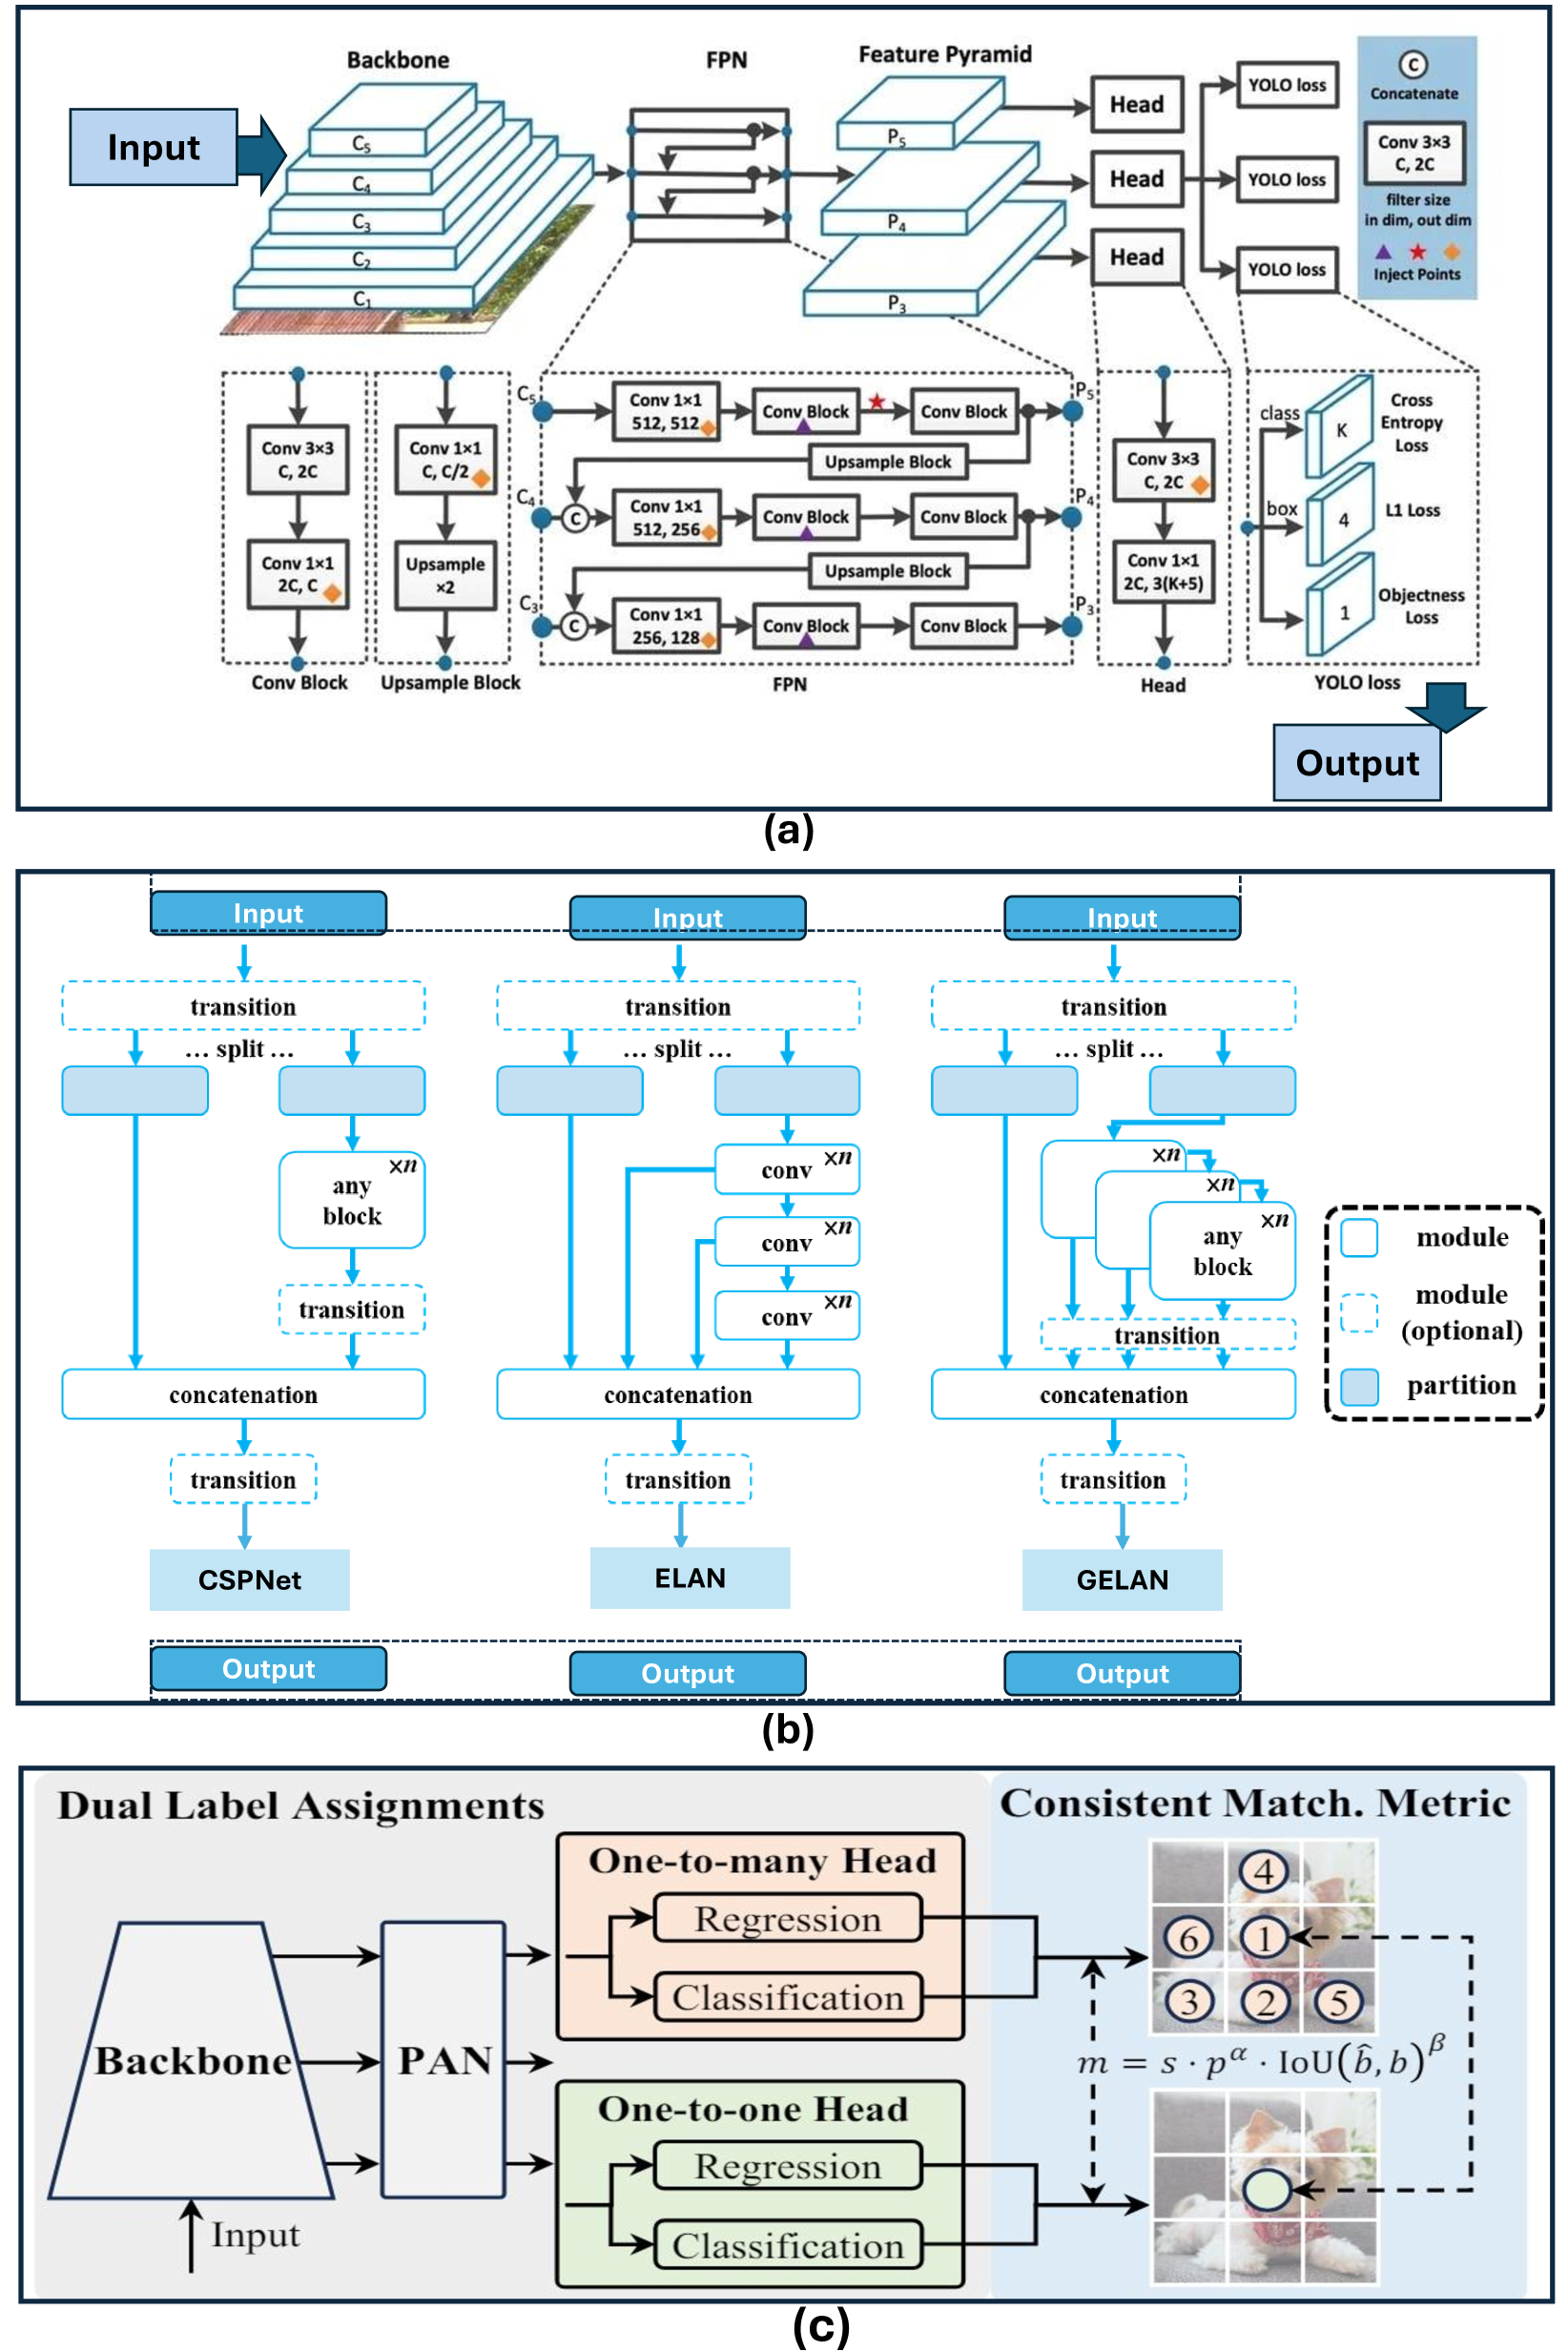
\includegraphics[width=0.8\textwidth]{figuras/arquitecture YOLO/v8_v9_v10.png}
  \caption{Diagramas de arquitectura de YOLOv8, YOLOv9 y YOLOv10}
  \label{fig:Yolov8_v9_v10_arquitectures}
  (a) YOLOv8 presenta una estructura principal basada en CSP, un cabezal desacoplado y libre de anclajes (\textit{anchor-free}), y una Red de Pirámide de Características (FPN) optimizada para una extracción eficiente de características a múltiples escalas. 
  (b) YOLOv9 integra la Información de Gradiente Programable con GELAN para una agregación robusta de características.
  (c) YOLOv10 presenta una estrategia de asignación dual, cabezales ligeros y un submuestreo desacoplado de canal espacial para mejorar la \textit{precision} y velocidad de la inferencia.
\end{figure}

\begin{itemize}
  \item \textbf{YOLOv11:} Se enfoca en mejorar la extracción de características mediante el bloque C3k2, el módulo \textit{Spatial Pyramid Pooling-Fast} (SPPF) y la Atención Espacial Paralela (C2PSA). Estas mejoras le permiten un rendimiento más preciso, especialmente en escenarios con objetos ocluidos \cite{defyolos} (\autoref{fig:Yolov11_v12_arquitectures}).
  \item \textbf{YOLOv12:} Su principal innovación es el módulo de Atención de Área (A²), que ajusta dinámicamente el campo receptivo para capturar señales contextuales globales y locales con un costo computacional mínimo. Esto, junto con la red R-ELAN, optimiza la fusión de características y aumenta drásticamente la velocidad de inferencia \cite{defyolos} (\autoref{fig:Yolov11_v12_arquitectures}).
\end{itemize}

\begin{figure}[htbp]
  \centering
  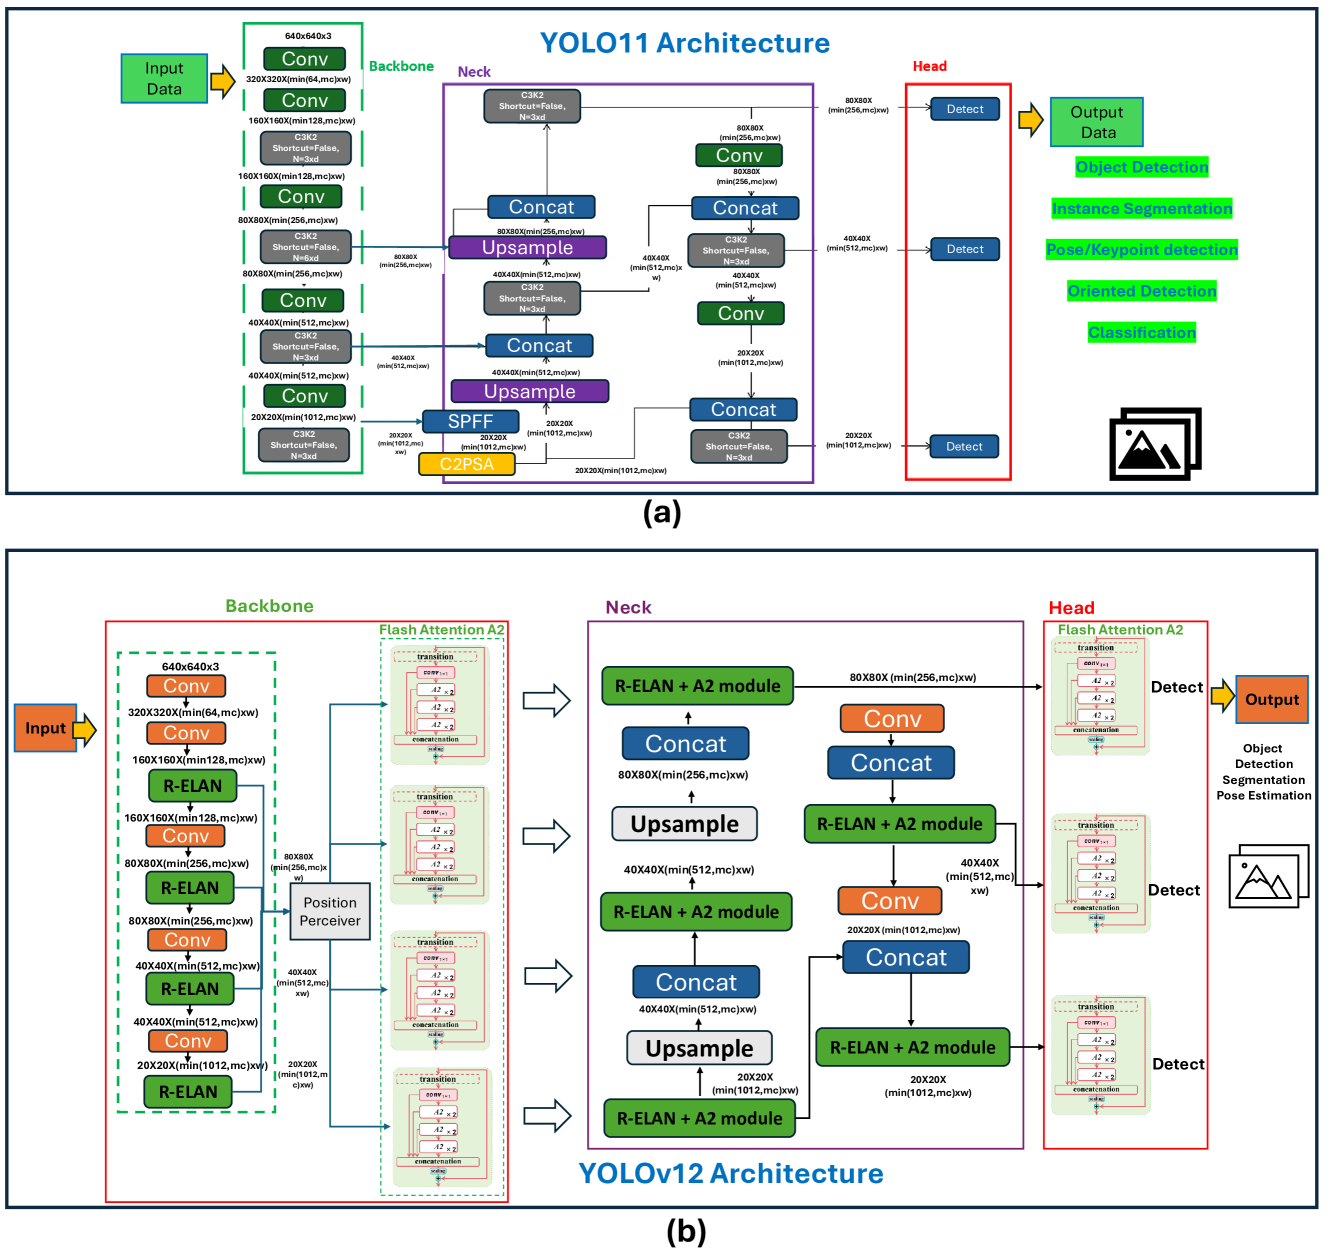
\includegraphics[width=0.85\textwidth]{figuras/arquitecture YOLO/v11_v12.png}
  \caption{Diagramas de arquitectura de YOLOv11 y YOLOv12}
  \label{fig:Yolov11_v12_arquitectures}
  (a) YOLOv11 utiliza una arquitectura mejorada que incluye bloques C3k2, SPPF y C2PSA. Estos componentes optimizan la extracción de características en diversas escalas y mejoran la atención espacial, lo que se traduce en una mayor precisión de detección.
  (b) YOLOv12 avanza sobre este diseño con una arquitectura centrada en la atención. Al integrar módulos de \textit{Area Attention} y bloques R-ELAN, optimiza la combinación de características, logrando un aumento drástico en la velocidad de inferencia para una detección de objetos en tiempo real de vanguardia.
\end{figure}

\subsection{Técnicas de optimización y validación de modelos}

Es bien conocida la existencia de diferentes tecnologías para asegurar la robustez y maximizar el rendimiento de los modelos. Algunas de estas tecnologías, son las siguientes:

\begin{itemize}
  \item \textbf{Optimización de hiperparámetros (Optuna):} El \textit{framework} Optuna \cite{optuna_github}, de optimización automática de hiperparámetros (tales como la tasa de aprendizaje, el \textit{momentum} o regulación), 
  explora de manera inteligente y eficiente el espacio de búsqueda y, al final, devuelve la mejor combinación de hiperparámetros encontrada. Se fundamenta en algoritmos de muestreo bayesiano y mecanismos de poda (\textit{pruning}) 
  que descartan de manera anticipada los ensayos poco prometedores.
  \item \textbf{Aumento de datos (\textit{data augmentation}):} Para mejorar la capacidad de generalización de un modelo y reducir el riesgo de sobreajuste (\textit{overfitting}) en conjuntos de datos limitados se recurre a esta técnica. 
  Esta permite generar nuevas muestras de entrenamiento aplicando transformaciones geométricas (rotaciones, traslaciones, escalado, etc.) y fotométricas (cambios de brillo, contraste, etc.) sobre las imágenes originales, 
  incrementando así la diversidad del conjunto de datos.
  \item \textbf{Validación cruzada (\textit{cross validation}):} Dentro de sus múltiples variantes, la más común consiste en dividir el conjunto de datos en K subconjuntos o pliegues. El modelo se entrena K veces, 
  utilizando en cada iteración un pliegue diferente para la validación y los K-1 restantes para el entrenamiento. El rendimiento final se calcula como la media de los resultados de las K iteraciones, proporcionando una medida de la capacidad 
  de generalización del modelo menos dependiente de una única división de datos. Esta técnica permite conocer si un modelo es fiable y robusto.
  \item \textbf{Ensamblado de modelos (\textit{ensemble}):} Esta técnica avanzada busca mejorar la precisión y la robustez de las predicciones combinando las salidas de múltiples modelos entrenados de forma independiente. 
  La hipótesis subyacente es que los errores de un modelo pueden ser compensados por los aciertos de otros (mediante el promedio o la ponderación de las predicciones individuales), especialmente si los modelos son diversos.
\end{itemize}

\subsection{Literatura de la investigación}

La inteligencia artificial (IA), y en particular el aprendizaje profundo (\textit{Deep Learning}), están transformando el campo de análisis de imágenes médicas en especialidades como la oncología, la neurología y la oftalmología.

En el ámbito de la andrología, la inteligencia artificial está comenzando a tomar especial relevancia en tareas como la concentración y recuento de espermatozoides, motilidad espermática, morfología espermática, integridad del ADN espermático, entre otras \cite{PannerSelvam}. En el contexto del análisis seminal, la mayor parte de las investigaciones se centran
en la automatización del análisis morfológico de los espermatozoides, desarrollando modelos capaces de identificar con alta precisión diferentes partes de la estructura celular (como cabeza, parte intermedia y cola) \cite{Maalej2025}.

Sin embargo, este proyecto presenta un desafío diferente y menos explorado, que a diferencia del análisis morfológico que se centra en un único tipo de célula,
la detección de células redondas, como ya se ha visto anteriormente, implica identificar un grupo heterogéneo de células (principalmente leucocitos y células germinales inmaduras) en un entorno complejo y "ruidoso" \cite{OMS}\cite{BJBS}.
La dificultad de identificar estas células redondas, incluso para expertos, y la subjetividad de los métodos manuales tradicionales \cite{Johanisson2000} justifican la necesidad de desarrollar herramientas automatizadas.

Este Trabajo de Fin de Máster se fundamenta en una innovadora POC previa, desarrollada por el grupo de investigación GVIS de la Universidad de León en colaboración con la empresa Microptic S.L. \cite{microptic}, en el marco del proyecto europeo DIGIS3 \cite{digis3}. 
Dicha prueba de concepto tuvo como objetivo validar la viabilidad de utilizar modelos de \textit{Deep Learning} para la identificación de células redondas en imágenes de semen humano. En ese trabajo inicial, se reentrenaron tres variantes del modelo YOLOv7 utilizando un conjunto de 
alrededor de 400 imágenes, logrando resultados prometedores en diferentes métricas. Este hito demostró que los detectores de objetos en tiempo real podían ser adaptados con éxito a esta tarea específica a pesar de las dificultades que esto supone.

Este hito sirve de precedente para explorar nuevas y mejoradas arquitecturas y poder superar las métricas obtenidas. Investigaciones de vanguardia han desarrollado modelos de alta precisión para identificar específicamente espermátidas redondas humanas, 
aunque utilizando muestras purificadas mediante citometría de flujo, lo que simplifica el problema al eliminar el "ruido" de fondo \cite{roundsCellsSpermatid}.

Por otro lado, trabajos como el modelo ACTIVE abordan un escenario más similar al de este proyecto, al detectar espermatozoides e "impurezas" en videos microscópicos sin procesar \cite{chen2024}. Los resultados para la detección de espermatozoides son realmente buenos, sin embargo, no se puede decir lo mismo
para las impurezas (todos los objetos presentes en la muestra que no son espermatozoides). Los propios autores admiten que, en algunos casos, incluso para expertos es difícil distinguir si un objeto
es una impureza o un espermatozoide. Esto introduce ambigüedad en los datos de entrenamiento perjudicando el aprendizaje del modelo, especialmente para la clase más difícil de definir ("impurezas") \cite{chen2024}.

En síntesis, este proyecto da continuidad al desarrollo tecnológico a partir de la prueba de concepto inicial, además de integrar y buscar superar los desafíos identificados en la literatura científica más reciente. La prueba de concepto sirve como precedente para dar continuidad y actualizar las 
arquitecturas para el problema de la detección de células redondas en muestras de semen humano, mientras que la literatura reciente pone de manifiesto los desafíos y dificultades en la detección de células heterogéneas. 


\subsection{Hipótesis de trabajo}

Considerando el potencial de las arquitecturas YOLO y las diferentes técnicas de optimización, se considera que mediante la exploración de las arquitecturas YOLO que van desde la versión 8 a la 12, 
junto con el diseño personalizado y la optimización de hiperparámetros, se consiga igualar o mejorar los modelos de la anterior prueba de concepto del grupo GVIS, 
en las métricas mAP y velocidad de inferencia. 

Adicionalmente, se espera que gracias a la arquitectura en desarrollo de YOLOv12 que incorpora mecanismos de atención, el algoritmo no identifique 
como células redondas a los anillos de Newton. La integración de estos modelos con la herramienta web sirva no solo como método de validación final, sino que también demuestre la viabilidad del sistema 
para que sea utilizado en un marco clínico real por personal experto.

\section{Definición del problema}
\label{sec:Definición del problema}

La problemática que da origen a este proyecto no es otra que la ardua y extenuante tarea que le supone a un experto la revisión manual de imágenes médicas de muestras de semen.

Por esta razón, el problema central que aborda este proyecto es diseñar, desarrollar y evaluar un sistema inteligente capaz de automatizar la detección de células 
redondas sobre un conjunto de imágenes médicas de muestras de semen, utilizando para ello técnicas de visión por computador (\textit{Computer Vision}) y aprendizaje profundo (\textit{Deep Learning}).

Este sistema inteligente debe ser capaz de procesar imágenes microscópicas como las de la \autoref{fig:Muestra de semen humano sin anotaciones}, donde las células objetivo coexisten con una densa población de espermatozoides, diversos artefactos visuales (Anillos de Newton)
y restos residuales ajenos al análisis. Asimismo, la dificultad que supone la distinción de células redondas de otros elementos morfológicamente similares (espermatozoides sin cola), esferas de las que se desconoce qué son, etc.

\begin{figure}[H]
  \centering
  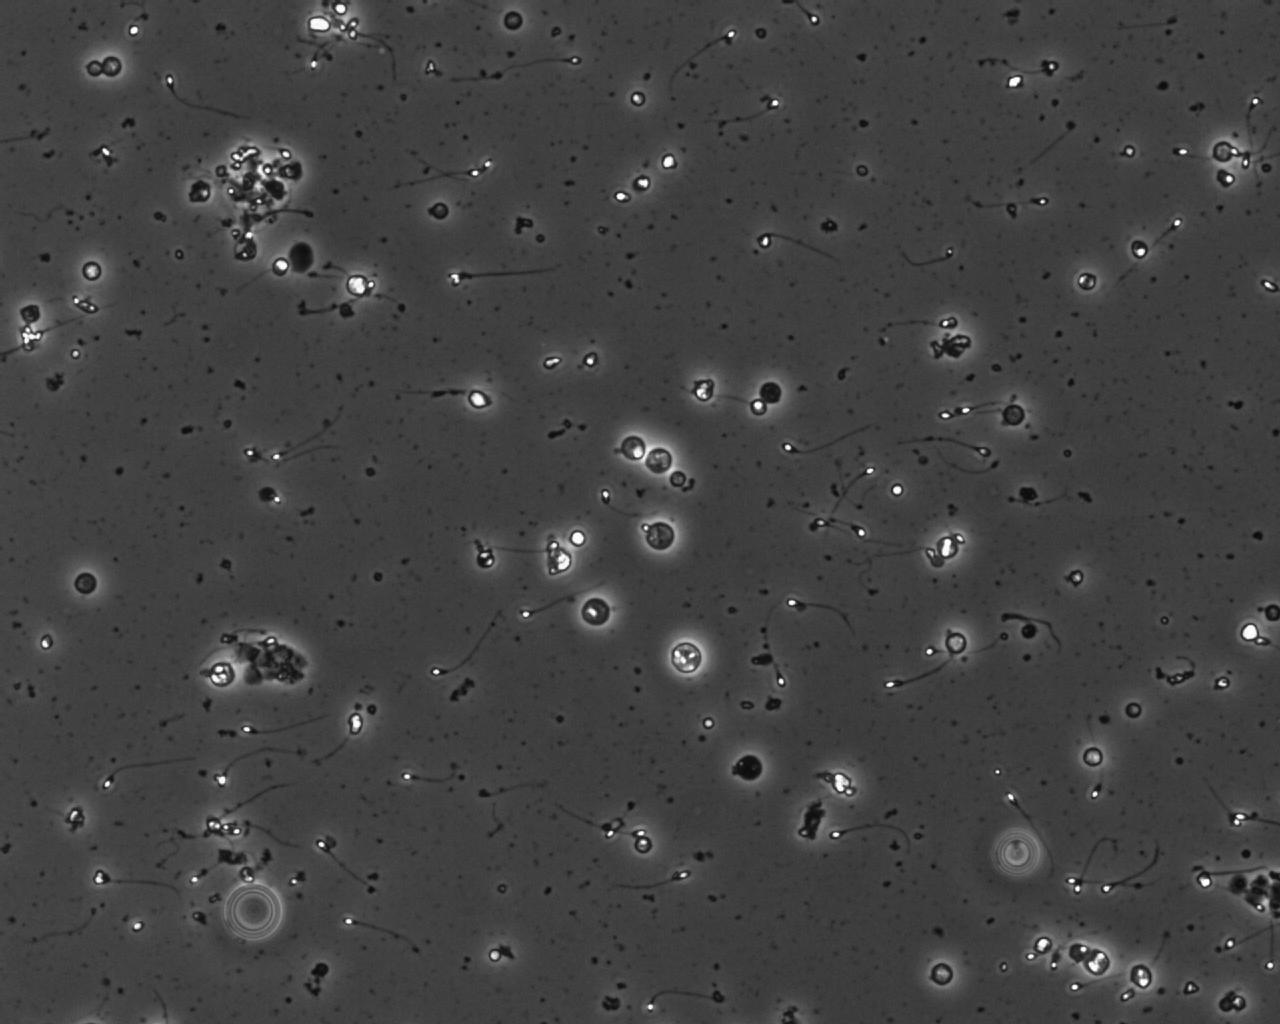
\includegraphics[width=0.8\textwidth]{figuras/rounds_cells/61.jpg}
  \caption{Muestra de semen humano sin anotaciones.}
  \label{fig:Muestra de semen humano sin anotaciones}
\end{figure}

La tarea de anotar el dataset presentó una dificultad intrínseca significativa, convirtiéndose en una fuente recurrente de complicaciones durante el desarrollo. 

La \autoref{fig:Anillos_Newton} anotada por un experto presenta la problemática de los anillos de Newton. Se verá posteriormente cómo afectan estos objetos a la correcta identificación de células redondas.

\begin{figure}[H]
  \centering
  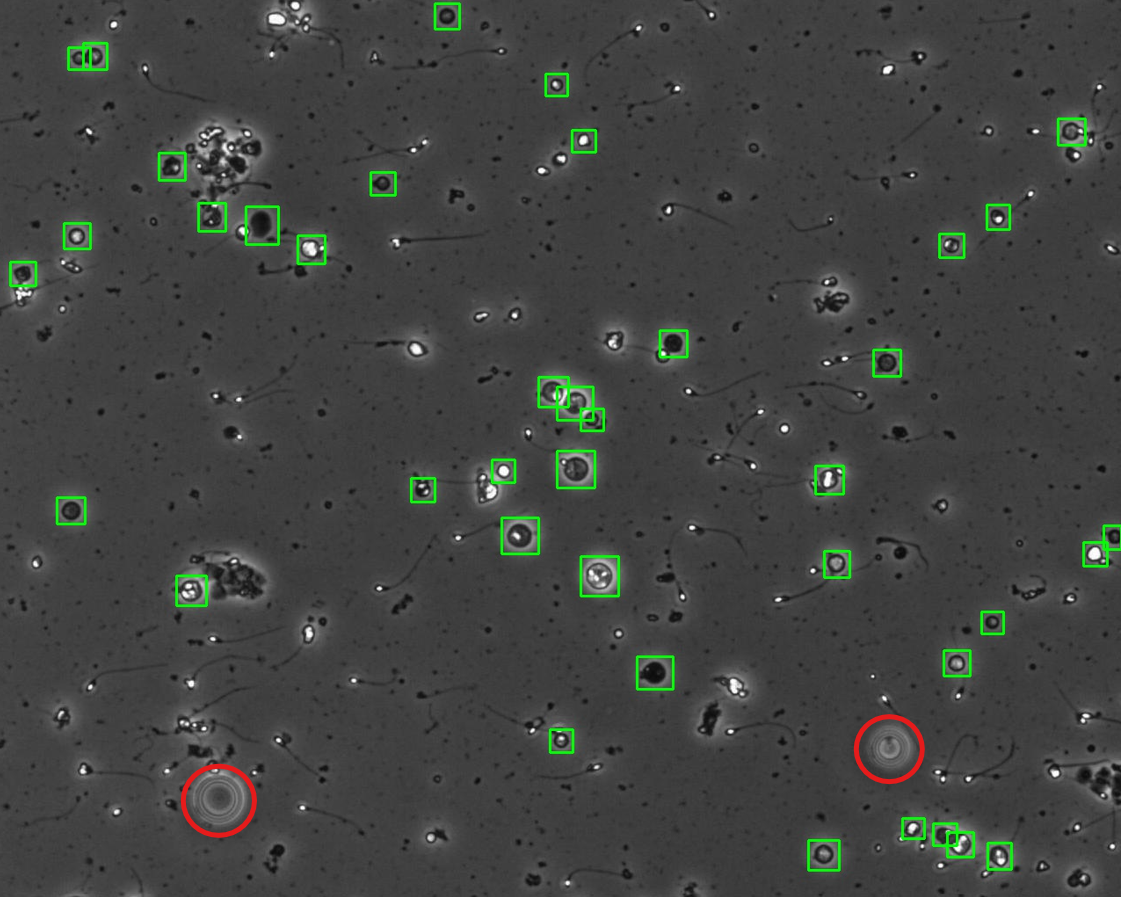
\includegraphics[width=0.8\textwidth]{figuras/rounds_cells/Anillos de Newton.png}
  \caption{Ilustración con anillos de Newton.}
  \label{fig:Anillos_Newton}
  Las \textit{bounding boxes} corresponden con las células redondas y los círculos rojos con los anillos de Newton.
\end{figure}

Asimismo, la \autoref{fig:feedback_experto} ilustra la ambigüedad inherente al proceso de anotación, un desafío corroborado por el feedback de los expertos de Microptic. El análisis de los especialistas 
revela que, si bien algunas anotaciones son correctas, existe una notable confusión al diferenciar las células redondas de otras estructuras visualmente similares, 
como espermatozoides con restos de citoplasma o cabezas de espermatozoides sin cola.

De manera crucial, se destacó que la correcta caracterización de ciertas células no es posible mediante la simple inspección visual y 
requiere de un análisis morfológico o citológico más exhaustivo \cite{OMS}.

Esto evidencia, una vez más, el alto grado de complejidad que supone anotar este tipo de imágenes médicas, incluso dentro del marco de recomendaciones de la OMS \cite{OMS} \cite{BJBS}.

\begin{figure}[H]
  \centering
  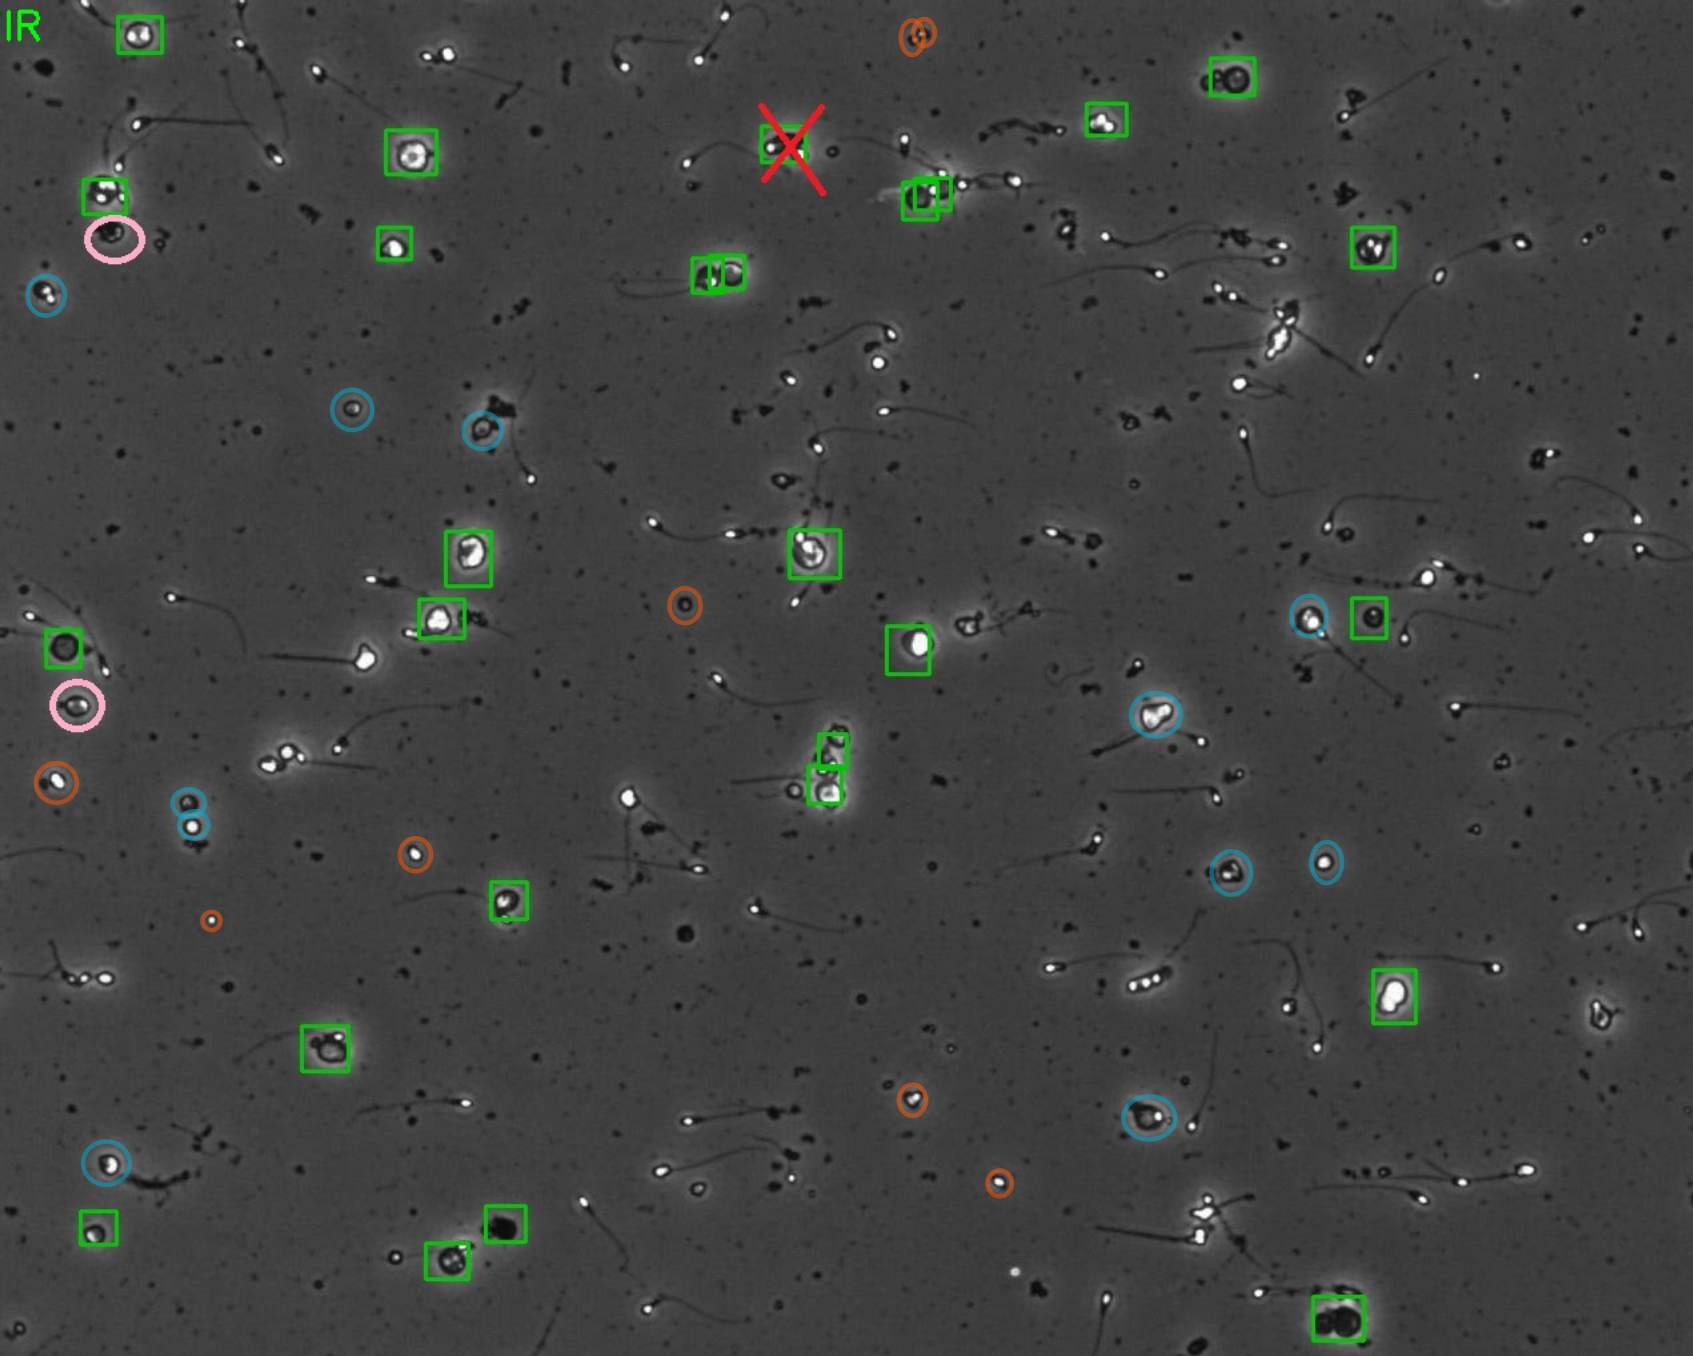
\includegraphics[width=0.8\textwidth]{figuras/rounds_cells/feedback_experto.png}
  \caption{Ilustración de anotaciones para \textit{feedback} con experto.}
  \label{fig:feedback_experto}
  La mayoría de células marcadas con los rectángulos verdes son ciertas células redondas. Los círculos rosas también son células redondas (probablemente germinales, pero es necesario un análisis morfológico específico para saberlo).
  Los círculos azules marcan correctamente algunas células redondas pero también indican espermatozoides que retienen la mayor parte del citoplasma (esferas grises con un área blanca bien contrastada).
  Muchos de los círculos naranjas son cabezas de espermatozoides sin cola y las esferas más pequeñas se desconoce que pueden ser.
\end{figure}

\chapter{Gestión de proyecto \textit{software}} %%%%%%%%%%%%%%%%%%%%%%%%%%%%%%%%%%%%%%%%%%%%%%%%%%%%%%%
\label{Gestión de proyecto software}

En este capítulo se definen las tareas a realizar durante el desarrollo,
se establece un cronograma y se detalla el presupuesto estimado para la realización del proyecto.

\section{Alcance del proyecto}
\label{sec:Alcance del proyecto}

\subsection{Definición del proyecto}
\label{sec:Definición del proyecto}

El presente Trabajo de Fin de Máster se centra en el diseño, desarrollo y validación de un sistema inteligente 
para la detección automatizada de células redondas en imágenes médicas de muestras de semen humano. 
Este proyecto, desarrollado en colaboración con la empresa Microptic S.L., 
aborda un desafío clave en el campo de la andrología: la necesidad de optimizar y estandarizar el análisis seminal.

Para abordar esta problemática, se desarrolla una solución de \textit{software} basada en aprendizaje profundo, cuyo objetivo es automatizar 
la detección de células redondas. El alcance se centra en la definición y desarrollo de una prueba de concepto que valida la viabilidad de 
esta solución tecnológica en un contexto clínico y de investigación.

Para ello, el proyecto abarca desde la gestión y preprocesamiento de los diferentes conjuntos de datos proporcionados por Microptic S.L.,
hasta el entrenamiento y evaluación de las diferentes arquitecturas de modelos de detección de objetos de YOLO. 
Como resultado final, se obtiene una herramienta web funcional que permite a los especialistas interactuar con el sistema de inteligencia artificial, 
obteniendo detecciones de células redondas sobre imágenes médicas 
de semen humano en tiempo real y, como consecuencia, optimizando el proceso de análisis seminal.

\subsection{Presupuesto}
\label{sec:Presupuesto}

El presupuesto del proyecto es una estimación que engloba todos los costes asociados a los recursos necesarios para 
alcanzar los objetivos definidos. Se realiza una valoración económica para simular un entorno profesional y poner valor del trabajo realizado.
Los costes se dividen en las siguientes categorías:

\subsubsection{Coste de personal}
\label{Coste de personal}
Los costes personales radican en la necesidad de contratar a un ingeniero informático que se encargue del
desarrollo técnico del proyecto, así como un \textit{Scrum Master} que supervise el flujo de trabajo 
y asegure el cumplimiento de los objetivos. 

\begin{itemize}
  \item \textbf{Ingeniero Informático:} en España, el sueldo medio de un ingeniero informático es de 30.004,24 \euro{} anuales, según 
  el XIX Convenio TIC \cite{ilerna_sueldo_ingeniero}. En un supuesto de un ingeniero junior con una jornada laboral de 40 horas semanales (1922 horas anuales), se traduce en un coste por hora de 
  15,61 \euro{}/hora.
  \item \textbf{\textit{Scrum Master}:} en España, el salario base medio es de 43.000,00 \euro{} anuales, según los
  datos de "glassdoor" \cite{glassdoor_scrum_master}. En un supuesto de jornada laboral de 40 horas semanales, esto se traduce en un coste por hora de 
  22,37 \euro{}/hora.
\end{itemize}

En la \autoref{tab:presupuesto_personal} se detalla el presupuesto estimado para los recursos humanos.

\begin{table}[H]
\caption{Presupuesto para los recursos humanos}
\label{tab:presupuesto_personal}
\centering
\resizebox{\textwidth}{!}{%
\renewcommand{\arraystretch}{1.3}
\begin{tabular}{lccccr}
\hline
\textbf{Puesto de trabajo} & \textbf{Horas semanales} & \textbf{Horas totales} & \textbf{Salario (\euro{}/hora)} & \textbf{Total} \\
\hline
Ingeniero Informático & 25 & 300 & 15,61 & 4683,00\euro{} \\
Srum Master & 3 & 18 & 22,37 & 402,66\euro{} \\
\hline
\textbf{Total} & & & & \textbf{5085,66\euro{}} \\
\hline
\end{tabular}
}

\end{table}

% \subsubsection{Coste del \textit{hardware}}
% \label{Coste del hardware}

% El coste del \textit{hardware} se refiere a los gastos asociados ejecución del proyecto. En este caso, se ha optado por emplear el siguiente recurso:

% \begin{itemize}
%   \item \textbf{Equipo para el Ingeniero Informático:} el coste de un ordenador con las características
%   descritas en la \autoref{sec:hardware_local} es de 765,00\euro{} (según los precios de la web de 
%   Lenovo en 2022).
%   \item \textbf{Equipo para el \textit{Scrum Master}:} el coste de un ordenador con las caracterísiticas básicas para ofimática 
%   es de 500,00\euro{}.
%   \item \textbf{Servidor privado:} el arredamiento de un servidor privado con las caracterísitcas descritas
%   en la \autoref{sec:servidor_privado} y mantenimiento incluido, tiene un coste de 0,29\euro{}/hora \cite{T4_pricing}. 
% \end{itemize}

% \begin{table}[H]
% \centering
% \caption{Desglose de costes de \textit{hardware}}
% \label{tab:coste_hardware}
% \renewcommand{\arraystretch}{1.2}
% \begin{tabular}{lcc}
% \hline
% \textbf{Concepto} & \textbf{Cantidad} & \textbf{Coste} \\
% \hline
% Equipo Ingeniero Informático & 1 & 765,00 \euro{} \\
% Equipo \textit{Scrum Master}          & 1 & 500,00 \euro{} \\
% Servidor privado (0,29\,\euro{}/h $\times$ 25 h) & 25 h & 7,25 \euro{} \\
% \hline
% \textbf{Total} & & \textbf{1272,25\euro{}} \\
% \hline
% \end{tabular}
% \end{table}

\subsubsection{Coste de \textit{software} y licencias}
\label{Coste de software y licencias}

Para el desarrolo del proyecto se aconseja el empleo de \textit{software} y herramientas específicas que faciliten
y optimicen el desarrollo del trabajo. En este caso, se opta por emplear GitHub Copilot, una herramienta
de Microsoft \cite{github_copilot}. El coste de esta herramienta se recoge en la \autoref{tab:presupuesto_hardware}.

\begin{table}[H]
\caption{Presupuesto para los recursos de \textit{hardware}}
\label{tab:presupuesto_hardware}
\centering
\renewcommand{\arraystretch}{1.2}
\begin{tabular}{lccc}
\hline
\textbf{Concepto} & \textbf{Precio mensual} & \textbf{Meses} & \textbf{Total} \\
\hline
GitHub Copilot & 10,00\euro{} & 3 & 30,00\euro{} \\

\hline
\end{tabular}
\end{table}

\subsubsection{Costes indirectos}

Los costes indirectos son aquellos gastos que no se pueden asignar directamente a la tarea
del proyecto pero que son necesarios para su ejecución, como puede ser el 
material de oficina. Entre estos, están los ordenadores para el \textit{Scrum Master} y el ingeniero informático y el servidor privado que forman parte
del equipo estándar de la institución. Se ha imputado un $5\%$ de los costes directos.

\subsubsection{Costes generales}

Son los gastos necerasios para el funcionamiento de la empresa, independientemente de los proyectos que tenga en marcha. Dentro de estos se incluyen internet, agua, limpieza, luz, etc.
Se establece un coste del $15\%$ sobre los costes directos.

\subsubsection{Beneficio industrial}

El beneficio industrial representa el margen de rentabilidad que la empresa establece por la ejecución del proyecto.
Este beneficio se calcula aplicando un porcentaje determinado ($12\%$) sobre la suma de los costes directos del proyecto.

\subsubsection{IVA}

El Impuesto sobre el Valor Añadido (IVA) es un tributo indirecto que grava el consumo de bienes y servicios. 
En el contexto de este proyecto, se aplica sobre la base imponible total, la cual incluye la suma de todos los costes (directos e indirectos) y el beneficio industrial.

Conforme a la legislación vigente, para las prestaciones de servicios que engloba este proyecto, se aplicará el tipo general de IVA, que se sitúa en el $21\%$ \cite{AEAT_IVA2025}.

\subsubsection{Coste total}
A continuación, se presenta un resumen del presupuesto total estimado para la realización del proyecto. 
Se desglosa en función de los costes de personal, \textit{software} y licencias, los cuales constituyen
los costes directos del proyecto, así como los costes indirectos y generales asociados.

\begin{table}[H]
\caption{Presupuesto final del proyecto}
\centering
\renewcommand{\arraystretch}{1.25}
\begin{tabular}{lcr}
\hline
\textbf{Tipo de presupuesto} & \textbf{Porcentaje} & \textbf{Coste} \\
\hline
Costes personal                 &          & 5.085,66\euro{} \\
Costes software                 &          & 30,00\euro{} \\
\hline
\textbf{Costes directos}       &          & \textbf{5.115,66\euro{}} \\
Costes indirectos     & 5\,\%    & 225,78\euro{} \\
Costes generales      &  15\,\%  & 767,35\euro{} \\
Beneficio industrial  & 12\,\%   & 613,88\euro{} \\
\hline
\textbf{Subtotal}     &          & \textbf{6.722,67\euro{}} \\
IVA aplicable         & 21\,\%   & 1.411,76\euro{} \\
\hline
\textbf{Total}        &          & \textbf{8.134,43\euro{}} \\
\hline
\end{tabular}
\label{tab:presupuesto_final}
\end{table}

El presupuesto de ejecución por los servicios contratados asciende a un total de 8.134,43\euro{} (\autoref{tab:presupuesto_final}).

\section{Plan de trabajo}
\label{Plan de trabajo}

En esta sección se detalla la estrategia y organización temporal para la ejecución del proyecto.

\subsection{Metodología}
\label{Metodología}

Para la gestión y desarrollo de este proyecto, se ha optado por una metodología ágil basada en Scrum \cite{scrum_org_what_is_scrum}.
Este marco de trabajo promueve la entrega incremental de resultados a través de iteraciones cortas y frecuentes, conocidas como sprints, 
lo que aporta una gran flexibilidad para adaptarse a los desafíos técnicos inherentes al desarrollo de un sistema de visión artificial 
para la detección de células redondas.

Los sprints para este proyecto tienen una duración de dos semanas, lo que permite un equilibrio adecuado entre la planificación y la ejecución.

Dentro de los roles y responsabilidades, se define al tutor académico como \textit{Scrum Master} y al ingeniero informático como el desarrollador principal.

Para la organización y planificación de las tareas, el proyecto se estructura en torno a un \textit{Product Backlog} (pila de producto). Este \textit{backlog} está 
compuesto por historias de usuario, que representan cada una de las funcionalidades o tareas a desarrollar. Cada historia de usuario se define con los siguientes atributos:

\begin{itemize}
  \item Identificador (ID): Un código único para referenciar y realizar el seguimiento de cada tarea.
  \item Título: Un nombre conciso y descriptivo que resume el objetivo.
  \item Descripción: Un párrafo que explica con claridad qué trabajo se debe realizar.
  \item Criterios de aceptación: Una lista de condiciones específicas y verificables que deben cumplirse para que la tarea se considere completada.
\end{itemize}

\subsection{Identificación de tareas}
\label{Identificación de tareas}

Atendiendo a la metodología Scum del proyecto, se definen las siguientes historias de usuario, que se detallan de la \autoref{tab:usuario1} a la \autoref{tab:usuario6}.

\definecolor{turquoiseLight}{RGB}{64,224,208}

%SPRINT 1
\begin{table}[H]
\centering
\adjustbox{width=\textwidth,center}{%
\renewcommand{\arraystretch}{1.5}
\setlength{\tabcolsep}{6pt}
\begin{tabular}{|>{\columncolor{turquoiseLight!25}}m{2.5cm}|m{0.3cm}|>{\columncolor{turquoiseLight!25}}m{1.3cm}|p{10cm}|}
\hline
\textbf{ID} & 1 & \textbf{Título} & Planificación, configuración e investigación \\
\hline
\textbf{Descripción} & \multicolumn{3}{m{15cm}|}{Sentar las bases del proyecto, configurar el entorno de trabajo y comprender el estado del arte.} \\
\hline
\textbf{Criterios de aceptación} & \multicolumn{3}{m{15cm}|}{El entorno de desarrollo (local y remoto) debe estar completamente configurado y probado. Se debe completar una revisión de la literatura sobre modelos de detección de objetos y análisis de imágenes médicas. El plan de proyecto y el análisis de riesgos deben estar documentados.} \\
\hline
\end{tabular}%
}
\caption{Historia de usuario 1 (Planificación, configuración e investigación)}
\label{tab:usuario1}
\end{table}

%SPRINT 2
\begin{table}[H]
\centering
\adjustbox{width=\textwidth,center}{%
\renewcommand{\arraystretch}{1.5}
\setlength{\tabcolsep}{6pt}
\begin{tabular}{|>{\columncolor{turquoiseLight!25}}m{2.5cm}|m{0.3cm}|>{\columncolor{turquoiseLight!25}}m{1.3cm}|p{10cm}|}
\hline
\textbf{ID} & 2 & \textbf{Título} & Preprocesamiento de datos y modelo base \\
\hline
\textbf{Descripción} & \multicolumn{3}{m{15cm}|}{Preparar el conjunto de datos para el entrenamiento y entrenar un primer modelo para establecer una línea de base.} \\
\hline
\textbf{Criterios de aceptación} & \multicolumn{3}{m{15cm}|}{El conjunto de datos debe estar completamente anotado y validado. El \textit{pipeline} de datos, incluyendo el aumento de datos, debe ser funcional. Se debe haber entrenado un modelo YOLO base y obtenido las primeras métricas de rendimiento para validar el proceso.} \\
\hline
\end{tabular}%
}
\caption{Historia de usuario 2 (Preprocesamiento de datos y modelo base)}
\label{tab:usuario2}
\end{table}

%SPRINT 3
\begin{table}[H]
\centering
\adjustbox{width=\textwidth,center}{%
\renewcommand{\arraystretch}{1.5}
\setlength{\tabcolsep}{6pt}
\begin{tabular}{|>{\columncolor{turquoiseLight!25}}m{2.5cm}|m{0.3cm}|>{\columncolor{turquoiseLight!25}}m{1.3cm}|p{10cm}|}
\hline
\textbf{ID} & 3 & \textbf{Título} & Entrenamiento y optimización \\
\hline
\textbf{Descripción} & \multicolumn{3}{m{15cm}|}{Entrenar y comparar diferentes arquitecturas de modelos, optimizando sus hiperparámetros para obtener el mejor rendimiento.} \\
\hline
\textbf{Criterios de aceptación} & \multicolumn{3}{m{15cm}|}{Se deben haber entrenado y evaluado al menos dos arquitecturas de modelos diferentes. La optimización de hiperparámetros debe estar completada y documentada. Se debe realizar una validación cruzada para asegurar la generalización y evitar el sobreajuste.} \\
\hline
\end{tabular}%
}
\caption{Historia de usuario 3 (Entrenamiento y optimización)}
\label{tab:usuario3}
\end{table}

%SPRINT 4
\begin{table}[H]
\centering
\adjustbox{width=\textwidth,center}{%
\renewcommand{\arraystretch}{1.5}
\setlength{\tabcolsep}{6pt}
\begin{tabular}{|>{\columncolor{turquoiseLight!25}}m{2.5cm}|m{0.3cm}|>{\columncolor{turquoiseLight!25}}m{1.3cm}|p{10cm}|}
\hline
\textbf{ID} & 4 & \textbf{Título} & Modelos avanzados y evaluación comparativa \\
\hline
\textbf{Descripción} & \multicolumn{3}{m{15cm}|}{Desarrollar y entrenar un modelo \textit{ensemble} y un modelo personalizado. Evaluar cuantitativamente todos los modelos (base, \textit{ensemble} y personalizado) para seleccionar el mejor.} \\
\hline
\textbf{Criterios de aceptación} & \multicolumn{3}{m{15cm}|}{El modelo \textit{ensemble} y el modelo personalizado deben estar implementados y entrenados. Se debe realizar una evaluación comparativa con métricas (mAP, precisión, \textit{recall}) y documentar los resultados para justificar la selección del modelo final.} \\
\hline
\end{tabular}%
}
\caption{Historia de usuario 4 (Modelos y evaluación comparativa)}
\label{tab:usuario4}
\end{table}

%SPRINT 5
\begin{table}[H]
\centering
\adjustbox{width=\textwidth,center}{%
\renewcommand{\arraystretch}{1.5}
\setlength{\tabcolsep}{6pt}
\begin{tabular}{|>{\columncolor{turquoiseLight!25}}m{2.5cm}|m{0.3cm}|>{\columncolor{turquoiseLight!25}}m{1.3cm}|p{10cm}|}
\hline
\textbf{ID} & 5 & \textbf{Título} & Desarrollo de la herramienta web interactiva \\
\hline
\textbf{Descripción} & \multicolumn{3}{m{15cm}|}{Diseñar, implementar y probar la herramienta web con \textit{Streamlit}, integrando los diferentes modelos de YOLO para permitir la detección de células en tiempo real.} \\
\hline
\textbf{Criterios de aceptación} & \multicolumn{3}{m{15cm}|}{La herramienta web debe ser completamente funcional: permitir la carga de imágenes (individuales y por lotes), seleccionar el modelo, visualizar las detecciones con \textit{bounding boxes}, mostrar métricas y permitir la descarga de resultados. La aplicación debe ser estable y estar documentada en el manual de usuario.} \\
\hline
\end{tabular}%
}
\caption{Historia de usuario 5 (Desarrollo de la herramienta web interactiva)}
\label{tab:usuario5}
\end{table}

%SPRINT 6
\begin{table}[H]
\centering
\adjustbox{width=\textwidth,center}{%
\renewcommand{\arraystretch}{1.5}
\setlength{\tabcolsep}{6pt}
\begin{tabular}{|>{\columncolor{turquoiseLight!25}}m{2.5cm}|m{0.3cm}|>{\columncolor{turquoiseLight!25}}m{1.3cm}|p{10cm}|}
\hline
\textbf{ID} & 6 & \textbf{Título} & Documentación final y entrega \\
\hline
\textbf{Descripción} & \multicolumn{3}{m{15cm}|}{Finalizar la redacción de la memoria del TFM y preparar todos los materiales para la entrega y defensa del proyecto.} \\
\hline
\textbf{Criterios de aceptación} & \multicolumn{3}{m{15cm}|}{La memoria del TFM debe estar completamente redactada, incluyendo todos los capítulos, anexos y bibliografía. El código del proyecto debe estar documentado y subido a un repositorio. La presentación para la defensa final debe estar preparada.} \\
\hline
\end{tabular}%
}
\caption{Historia de usuario 6 (Documentación final y entrega)}
\label{tab:usuario6}
\end{table}

\subsection{Estimación de tareas}
\label{Estimación de tareas}

Esta sección presenta la planificación del proyecto (\autoref{tab:estimacion_tareas}), detallando las tareas a realizar y el cronograma previsto para su ejecución.

\begin{table}[H]
\caption{Estimación de tareas del proyecto}
\centering
\adjustbox{width=\textwidth,center}{%
\renewcommand{\arraystretch}{0.8} % Aumenta el espaciado para mejor legibilidad
\setlength{\arrayrulewidth}{0.6pt}
% Definición de columnas para centrar verticalmente y ajustar anchos
\begin{tabular}{|c|m{4.5cm}|m{6cm}|c|}
\hline
\rowcolor{turquoiseLight!30}
\multicolumn{1}{|c|}{\textbf{ID}} & 
\multicolumn{1}{c|}{\textbf{Historia de usuario}} & 
\multicolumn{1}{c|}{\textbf{Tareas principales}} & 
\multicolumn{1}{c|}{\textbf{Semanas}} \\
\hline
1 & Planificación, configuración e investigación & 
- Investigación del estado del arte \newline - Configuración de entornos (local/remoto) \newline - Definición detallada del plan de proyecto y riesgos \newline - Análisis inicial del \textit{dataset} & 
24-25 \\
\hline
2 & Preprocesamiento de datos y modelo base & 
- Anotación, validación y aumento de datos \newline - Desarrollo del \textit{pipeline} de datos \newline - Entrenamiento y evaluación de un modelo inicial &
26-27 \\
\hline
3 & Entrenamiento y optimización & 
- Entrenamiento de múltiples arquitecturasYOLO \newline - Optimización de hiperparámetros \newline - Validación cruzada y análisis de resultados &
28-29 \\
\hline
4 & Modelos avanzados y evaluación &
- Desarrollo de modelo \textit{ensemble} \newline - Implementación de modelo personalizado \newline - Evaluación comparativa &
30-31 \\
\hline
5 & Desarrollo de la herramienta web & 
- Implementación del \textit{backend} (lógica de inferencia) \newline - Creación del \textit{frontend} (interfaz de usuario) \newline - Integración y pruebas funcionales &
32-33 \\
\hline
6 & Documentación final y entrega &
- Redacción de la memoria del TFM \newline - Documentación del código y repositorio &
34-35 \\
\hline
\end{tabular}
}
\label{tab:estimacion_tareas}
\end{table}


\subsection{Planificación de tareas}
\label{Planificación de tareas}

Atendiendo a la metodología agile Scrum, el desarrollo del proyecto se ha estructurado en seis \textit{sprints} de dos semanas cada uno.
Cada \textit{sprint} se corresponde con una historia de usuario, permitiendo un desarrolle lógico y secuencial.
En el anexo \autoref{Seguimiento de proyecto} se detalla mediante del diagrama de Gantt \cite{OnlineGantt2025} la planificación de cada \textit{sprint}, con una fecha final objetivo que corresponde con la entrega del día 5 de septiembre de 2025.
A continuación, se resume el enfoque de cada sprint:

\begin{itemize}[label=-]
  \item Planícación, configuración e investigación (Semanas 24-25): Esta fase inicial se centra en establecer las bases teóricas y técnicas del proyecto. Incluye una revisión del estado del arte, la configuración de los entornos de desarrollo (local y remoto) y un análisis inicial del \textit{dataset} para comprender sus características.
  
  \item Preprocesamiento de datos y modelo base (Semanas 26-27): Se prepararan los datos para el entrenamiento. Se revisan y gestionan los diferentes conjuntos de datos. Finaliza con el entrenamiento de un primer modelo que sirve como referencia.
  
  \item Entrenamiento y optimización (Semanas 28-29): Se entrenan y comparan las diferentes arquitecturas de YOLO. Se aplica la optimización de hiperparámetros y se utiliza la validación cruzada para asegurar que los modelos generalicen correctamente y no sufran de sobreajuste.
  
  \item Modelos avanzados y evaluación (Semanas 30-31): Se desarrolla un modelo \textit{ensemble} que combina las fortalezas de varios modelos y un modelos personalizado. Se realiza la evaluación comparativa final.
  
  \item Desarrollo de la herramienta web (Semanas 32-33): Se dedica por completo a la creación de la aplicación interactiva con \textit{Streamlit}. Se implementa tanto el backend (lógica de inferencia) como el frontend (interfaz de usuario).
  
  \item Documentación final y entrega (Semanas 34-35): La última fase se centra en consolidar todo el trabajo. Incluye la redacción final de la memoria del TFM y la documentación del código para garantizar su reproducibilidad.
\end{itemize}

\section{Gestión de recursos}
\label{Gestión de recursos}

La gestión de recursos implica la especificación, asignación y supervisión de los recursos necesarios para llevar a cabo el proyecto de manera eficiente.

\subsection{Especificación y asignación de recursos}
\label{Especificación y asignación de recursos}

Los recursos disponibles para el desarrollo de este proyecto se clasifican en tres grupos:

\begin{itemize}
  \item \textbf{Recursos económicos:} El presupuesto económico viene detallado en la \autoref{sec:Presupuesto}, y asciende a un total de 9.739,01\euro{}.
  \item \textbf{Recursos físicos:}
    \begin{itemize}[label=-]
      \item Equipo para Scrum Master
      \item Equipo para el desarrollador
      \item Servidor remoto con GPU Tesla T4 proporcionado por GVIS
      \item Instalaciones: luz, internet, material de oficina, etc
    \end{itemize}
  \item \textbf{Recursos humanos:} 
    \begin{itemize}[label=-]
      \item \textit{Scrum Master}: Tutor académico
      \item Desarrollador: Ingeniero Informático
      \item Experto de Microptic S.L.
      \item Soporte de infraestructura (GVIS): Provisión y operación del servidor remoto.
    \end{itemize}
\end{itemize}

La asignación de recursos se realiza de la siguiente manera: cada rol humano dispone del equipo informático necesario para sus 
funciones. El desarrollador utiliza su equipo local para el preprocesado de datos, desarrollo del \textit{pipeline} de metodológico y el desarrollo de la aplicación web con \textit{Streamlit}. 
El servidor remoto con GPU Tesla T4 se reserva para las tareas de mayor coste computacional, como el entrenamiento del modelo pesado (YOLOv12l).
Se solicita puntualmente una consulta con el experto de Microptic S.L. para resolver dudas técnicas en las anotaciones de las imágenes.
Finalmente, las instalaciones garantizan el soporte operativo (luz, internet) para todas las actividades.

\section{Gestión de riesgos}
\label{sec:Gestión de riesgos}

Se identifican, analizan y gestionan los riesgos potenciales que podrían afectar al desarrollo exitoso del proyecto.

\subsection{Identificación y análisis de riesgos}
\label{Identificación y análisis de riesgos}

Para una mayor claridad e interpretación, se elabora la \autoref{tab:analisis_riesgos} que detalla los riesgos identificados, su probabilidad de ocurrencia (prob.), el impacto potencial, 
las causas subyacentes y las estrategias de gestión propuestas.

\definecolor{turquoiseLight}{RGB}{64,224,208}

\begin{table}[H]
\caption{Análisis de riesgos del proyecto}
\centering
\adjustbox{width=\textwidth,center}{%
\renewcommand{\arraystretch}{1.3}
\setlength{\arrayrulewidth}{1.2pt}
% Se han cambiado las columnas 'p' por 'm' para centrar verticalmente
\begin{tabular}{|c|m{3cm}|c|c|c|m{5.5cm}|m{5.5cm}|}
\hline
\rowcolor{turquoiseLight!30}
\multicolumn{1}{|c|}{\textbf{ID}} & 
\multicolumn{1}{c|}{\textbf{Riesgo}} & 
\multicolumn{1}{c|}{\textbf{Categoría}} & 
\multicolumn{1}{c|}{\textbf{Probabilidad}} & 
\multicolumn{1}{c|}{\textbf{Impacto}} & 
\multicolumn{1}{c|}{\textbf{Causas}} & 
\multicolumn{1}{c|}{\textbf{Gestión}} \\
\hline
1 & Etiquetado subjetivo de células & Datos & Alta & Alto & 
Subjetividad en la identificación de células, generando inconsistencias en el etiquetado & 
Implementar validación y reetiquetado por expertos para consolidar un \textit{ground truth} robusto \\
\hline
2 & Artefactos confundidos con células & Datos & Baja & Bajo & 
Presencia de artefactos visuales (ej. anillos de Newton) que se confunden con células redondas & 
Elevar umbral de de confianza de los modelos y evaluarlos en imágenes con artefactos para seleccionar las mejores arquitecturas \\
\hline
3 & \textit{Dataset} limitado & Datos & Media & Alto & 
La calidad, cantidad o representatividad del \textit{dataset} puede ser insuficiente o contener sesgos & 
Aplicar técnicas de \textit{data augmentation} para incrementar la diversidad y mejorar la generalización \\
\hline
4 & Definición ambigua de objetivos &  Planificación & Media & Alto & 
Objetivos mal definidos o cambiantes que dificultan la planificación &
Revisión detallada y continuada de los objetivos\\
\hline
5 & Cambios no planificados en requisitos & Planificación & Baja & Medio & 
Cambios inesperados &
Gestión de cambios y documentación detallada\\
\hline
6 & Desviación en los plazos & Planificación & Alta & Medio & 
Estimaciones optimistas y retrasos en tareas críticas &
Monitorización continua\\
\hline
7 & Errores de código o integración & Implementación & Alta & Bajo & 
Escasez de pruebas, errores humanos & 
Realización continuada de pruebas y control de versiones \autoref{Control de versiones} \\
\hline
8 & Faltan recursos técnicos o humanos & Implementación & Alta & Bajo & 
Limitaciones de \textit{hardware} en el uso de GPU & 
Se priorizan modelos ligeros, se ajusta el \textit{batch size} a la VRAM disponible; se externaliza a un servidor privado \\
\hline
9 & Riesgo de \textit{overfitting} & Implementación & Media & Medio & 
Los modelos sobreajusten (overfitting) los datos de entrenamiento y no generalicen correctamente a nuevos conjuntos de imágenes & 
Empleo de pruebas de validación, técnicas de regularización y evaluación final sobre múltiples conjuntos de test para verificar la generalización \\
\hline
10 & Retrasos por complejidad técnica no prevista & Implementación & Media & Bajo & 
Subestimación de la complejidad, falta de experiencia & 
Reuniones breves de alineación, formación continuada para el equipo \\
\hline
11 & Presión presupuestaria & Externo & Baja & Alto & 
Costes de \textit{hardware} y \textit{software} puntuales & 
Definir un tope de gasto y priorizar ejecuciones críticas\\
\hline
12 & Eventos improvistos & Externo & Baja & Alto & 
Pandemia, apagón eléctrico o de internet, etc & 
Plan de contingencia local-remoto y seguro adecuado\\
\hline
13 & Dependencia de terceros & Externo & Media & Medio & 
Alquiler de GPU no disponible o retraso en entregas de \textit{hardware}, servidores caídos, etc & 
Diversificación de proveedores y contratos sólidos con cláusulas que penalizan el incumplimiento\\
\hline
\end{tabular}
}
\label{tab:analisis_riesgos}
\end{table}

\section{Legislación y normativa}
\label{Legislación y normativa}

En el marco de ejecución de este proyecto, se ha llevado a cabo un riguroso cumplimiento de la legislación y normativa vigente. A continuación, 
se detalla cómo el proyecto se ajusta y adhiere a las leyes pertinentes:

\begin{itemize}
    \item \textbf{Ley Orgánica 3/2018, de 5 de diciembre, de Protección de Datos Personales y garantía de los derechos digitales.}\cite{LOPD2018}
    
    Este proyecto respeta plenamente la Ley Orgánica 3/2018, la cual reconoce el derecho fundamental a la protección de datos personales. 
    La creación y tratamiento del \textit{dataset} de imágenes médicas se ha realizado conforme a las disposiciones de la ley, asegurando la legalidad en el tratamiento de datos biomédicos. 
    Se han obtenido los permisos explícitos necesarios para el uso de las imágenes, garantizando la privacidad y anonimización de los datos de los pacientes. 
    
    \item \textbf{Reglamento (UE) 2016/679 del Parlamento Europeo y del Consejo, de 27 de abril de 2016, relativo a la protección de las personas físicas en lo que respecta al tratamiento de datos personales y a la libre circulación de estos datos y por el que se deroga la Directiva 95/46/CE (Reglamento general de protección de datos).}\cite{RGPD2016}

    La creación y tratamiento del \textit{dataset} de imágenes médicas en este proyecto se ha realizado conforme a los principios del RGPD, garantizando la legalidad y transparencia en el 
    tratamiento de datos biomédicos. Todas las imágenes han sido previamente anonimizadas y se han implementado medidas técnicas y organizativas 
    para asegurar la seguridad y privacidad de los datos, cumpliendo así con las exigencias del RGPD para datos de salud considerados de categoría 
    especial.
    
    \item \textbf{Reglamento (UE) 2024/1689 del Parlamento Europeo y del Consejo, de 13 de junio de 2024, por el que se establecen normas armonizadas en materia de inteligencia artificial.}\cite{ReglamentoIA2024}

    Este reglamento establece normas armonizadas para garantizar la seguridad, ética y transparencia en el desarrollo y aplicación de sistemas de IA en la Unión Europea.  
    En el contexto de este TFM, el sistema desarrollado se considera una herramienta de investigación y apoyo a la evaluación biomédica. No está concebido ni validado para toma de decisiones clínicas autónomas,
    por lo que su uso actual no se presenta como IA de alto riesgo. No obstante, para alinearse con los requisitos se incorporan las siguientes medidas: documentación completa, evaluación de riesgos y validación, 
    trazabilidad y registro para una posterior reproducibilidad.
    
    \item \textbf{Real Decreto Legislativo 1/1996, de 12 de abril, por el que se aprueba el texto refundido de la Ley de Propiedad Intelectual, regularizando, aclarando y armonizando las disposiciones legales vigentes sobre la materia.}\cite{RDL1996}
    
    En conformidad con el Real Decreto Legislativo 1/1996, el proyecto respeta la normativa sobre propiedad intelectual. Se ha optado por utilizar 
    únicamente código y herramientas de \textit{software} libre y de código abierto para garantizar el cumplimiento de la normativa en materia de propiedad 
    intelectual.
\end{itemize}


\chapter{Metodología} %%%%%%%%%%%%%%%%%%%%%%%%%%%%%%%%%%%%%%%%%%%%%%%%%%%%%%%
\label{metodologia}

\section{Arquitecturas de la familia YOLO}
\label{Arquitecturas de la familia YOLO}

Como modelo base, se selecciona la familia de arquitecturas de YOLO. A lo largo del proyecto, se exploran y evaluan sistemáticamente las arquitecturas 
que van desde la versión 8 hasta la 12, aprovechando los avances y mejoras introducidas para determinar cual es mejor. La descripción de cada arquitectura
se recoge en la \autoref{sec:Arquitecturas}. 

Cabe destacar que, para cada versión, se entrenan los modelos ligeros (s) a excepción de la última versión YOLOv12 que se prueba con una versión más robusta (l) 
para evaluar el impacto del tamaño del modelo en las diferentes métricas (\autoref{sec:Métricas}) y velocidad de inferencia.

Para todas estas arquitecturas, se aplicó una estrategia de aprendizaje por transferencia (\textit{transfer learning}), utilizando pesos preentrenados en el conjunto de datos COCO \cite{COCO}.
Posteriormente se realizó un ajuste fino (\textit{fine-tuning}) con el \textit{dataset} específico de imágenes de células redondas para adaptar el conocimiento previo 
a la nueva tarea de detección.

\section{Modelo \textit{ensemble}}
\label{Modelo ensemble}

Para mejorar la capacidad de generalización y el rendimiento de la detección de células redondas, se implementa una estrategia de ensamblado de modelos mediante la técnica de \textit{Weighted Boxes Fusion (WBF)} \cite{repoTFM}. 

Tras analizar los primeros resultados cuantitativos y cualitativos, se seleccionan dos modelos individuales con diferentes pesos, para la construcción del \textit{ensemble}. YOLOv12 con sus capacidades 
para capturar información contextual se pondera con un peso de $0,6$ mientras que YOLOv10s, que destaca por su eficiencia y precisión en la localización, se pondera con un peso de $0,4$.

Asimismo, el proceso de ensamblado se realiza siguiendo los siguientes pasos:

\begin{itemize}
  \item Para cada imagen, se obtienen las predicciones de los modelos individualmente.
  \item Se normalizan las coordenadas de las cajas para garantizar compatibilidad.
  \item Se aplica el algoritmo de WBF que agrupa \textit{bounding boxes} similares de diferentes modelos y las fusiona mediante un promedio ponderado según: el peso asignado a cada modelo y la confianza de cada una de las predicciones individuales.
  \item Se aplica un umbral de confianza para eliminar aquellas predicciones con baja probabilidad.
\end{itemize}

Cabe destacar que, cuando las predicciones de YOLOv12 y YOLOv10 no coinciden (sin solapamiento significativo de las \textit{bounding boxes}), el algoritmo mantiene las detecciones como predicciones independientes,
aplica el umbral de omisión de cajas a cada predicción individual y si supera dicho umbral, estas predicciones se incluyen en el resultado final.

De este modo, se aprovechan las fortalezas de cada modelo y se reducen los falsos negativos al mantener detecciones únicas de cada modelo (mejora el \textit{recall}).

Para obtener la configuración óptima de hiperparámetros, se exploran diferentes valores en un \textit{grid}. Para el umbral de IoU (cuando dos \textit{bounding boxes} se consideran superposiciones de la misma detección) se exploran los valores 
de $0,3$, $0,4$ y $0,5$ y para el umbral de omisión de cajas (determina la confianza mínima para considerar una predicción) se exploran los valores de $0,25$, $0,3$ y $0,35$.

La configuración óptima resultante fue un umbral de IoU de $0,5$, un umbral de omisión de cajas de 0.35 y un umbral de IoU para cada modelo de 0.25.

\section{Modelo personalizado}
\label{Modelo personalizado}

Este modelo personalizado o \textit{custom} representa una arquitectura híbrida al combinar elementos específicos de tres generaciones de YOLOv8, YOLOv9 y YOLOv10. 

La arquitectura sigue el patrón típico de los modelos YOLO con una profundidad (controla el número de capas repetidas en la arquitectura) de $0,33$ y un factor de anchura 
(controla el número de canales (filtros) en cada capa convolucional de la red) de $0,50$, dando lugar a un equilibrio entre rendimiento y velocidad.

La arquitectura del modelo se segmenta en dos componentes clave:

\subsubsection{\textit{Backbone}}

Este componente es el responsable de la extracción de características e integra las siguientes capas:

\begin{table}[H]
\caption{Estructura del \textit{backbone} del modelo personalizado}
\centering
\resizebox{\textwidth}{!}{
\begin{tabular}{clccl}
\toprule
\textbf{Índice} & \textbf{Tipo} & \textbf{Canales} & \textbf{Stride} & \textbf{Función} \\
\midrule
0-1 & Conv & 64/128 & 2/2 & Extracción inicial de características \\
2 & C2f (YOLOv8) & 128 & 1 & Agregación eficiente de características a baja escala \\
3-4 & Conv + C2f & 256 & 2 & Captura de patrones a escala media \\
5-6 & SCDown (YOLOv10) + C2f & 512 & 2 & Preservación de información espacial \\
7 & SCDown (YOLOv10) & 1024 & 2 & Reducción contextual avanzada \\
8 & RepNCSPELAN4 (YOLOv9) & [1024,512,256,1] & 1 & Reparametrización para patrones complejos \\
9 & PSA & 1024 & 1 & Atención espacial píxel a píxel \\
\bottomrule
\end{tabular}
}
\end{table}

\subsubsection{\textit{Head}}
Responsable de interpretar las características y realizar la detección. Estructura FPN+PAN (\textit{Feature Pyramid Network + Path Aggregation Network}):

\begin{table}[H]
\caption{Estructura del \textit{head} del modelo personalizado}
\centering
\resizebox{\textwidth}{!}{
\begin{tabular}{clcl}
\toprule
\textbf{Índice} & \textbf{Tipo} & \textbf{Canales} & \textbf{Función} \\
\midrule
10-12 & Upsample + Concat + C2f & 512 & Ampliación y fusión con características P4 \\
13-15 & Upsample + Concat + C2f & 256 & Salida P3 para objetos pequeños \\
16-18 & Conv + Concat + C2f & 512 & Salida P4 para objetos medianos \\
19-21 & Conv + Concat + C2f & 1024 & Salida P5 para objetos grandes \\
22 & Detect & [nc] & Detección final a múltiples escalas \\
\bottomrule
\end{tabular}
}
\end{table}

Las características de este modelo son:

\begin{itemize}
  \item Uso de SCDown de YOLOv10 que preserva mejor la información espacial durante la reducción dimensional.
  \item Integración del módulo RepNCSPELAN4 de YOLOv9 para mejorar la capacidad de representación.
  \item Incorporación de atención espacial (PSA) para enfocarse en regiones relevantes.
  \item Estructura FPN+PAN optimizada para la detección a múltiples escalas.
\end{itemize}

\chapter{Experimentación} %%%%%%%%%%%%%%%%%%%%%%%%%%%%%%%%%%%%%%%%%%%%%%%%%%%%%%%
\label{Experimentación}

\section{\textit{Dataset}}
\label{sec:Dataset}
El \textit{dataset} inicial proporcionado por la empresa Microptic \cite{microptic} está constituido por un conjunto de \textit{train} y \textit{test} en formato PASCAL VOC.

\begin{table}[htbp]
\caption{Distribución del \textit{dataset} original}
\centering
\begingroup
\setlength{\tabcolsep}{8pt}
\small
\begin{adjustbox}{max width=\textwidth}
\begin{tabular}{l c c c c c}
\toprule
\textbf{Partición} & \textbf{Resoluciones (px)} & \textbf{Nº imágenes (resolución)} & \textbf{Nº imágenes} & \textbf{Sin instancias} & \textbf{Escala grises}\\
\midrule
\textit{Train} & \makecell[l]{1280\,×\,1024 \\ 768\,×\,616} & \makecell[r]{356 \\ 17} & 373 & 23 & 3 canales\\ 
\arrayrulecolor{gray!30}\specialrule{0.6pt}{0pt}{0pt}\arrayrulecolor{black}
\textit{Test}  & \makecell[l]{1280\,×\,1024 \\ 768\,×\,616} & \makecell[r]{87 \\ 7}   & 94  & 6  & 3 canales\\ 
\bottomrule
\end{tabular}
\end{adjustbox}
\endgroup
\label{tab:dataset_original}
\end{table}

El conjunto de datos inicial que nos proporciona Microptic \cite{microptic} está compuesto por 373 imágenes para \textit{train} y 94 para \textit{test}, de las cuales no presentan anotaciones: 23 imágenes de \textit{train} y 6 de \textit{test} (\autoref{tab:dataset_original}).
El conjunto de entrenamiento se divide utilizando la función \texttt{train\_test\_split} de \textit{scikit-learn}, reservando el $80\%$ (298 imágenes) para entrenamiento y el $20\%$ (75 imágenes) para validación. 
Esta división se realiza de forma aleatoria pero reproducible, fijando la semilla (\texttt{random\_state = 42}) para garantizar la consistencia de los resultados.

Adicionalmente, la empresa proporciona un conjunto de datos del \textit{test} reevaluado por expertos del dominio. Este conjunto se reetiqueta utilizando la herramienta \textit{LabelImg} \cite{labelimg_github} en formato PASCAL VOC. 
Las correcciones afectan a un total de 60 imágenes, incrementando el número de instancias de 1273 a 1412.

Asimismo, se incluyeron dos conjuntos adicionales denominados \textit{test2} y \textit{test3}, inicialmente sin anotaciones pero que contenían \textit{bounding boxes} generados por modelos YOLO \cite{ultralytics_models} preentrenados 
por el grupo GVIS de la Universidad de León. Estas predicciones fueron posteriormente corregidas y validadas por expertos, proporcionando dos conjuntos adicionales para evaluación. 
La composición final del \textit{dataset} se presenta en la \autoref{tab:dataset_final}.

\begin{table}[htbp]
\caption{Resumen del \textit{dataset} de actuación}
\centering
\rowcolors{2}{gray!12}{white}
\begin{tabular}{l c c c c c}
\toprule
\textbf{Partición} & \textbf{Imágenes} & \textbf{Instancias} & \textbf{1280$\times$1024} & \textbf{768$\times$616} & \textbf{Escala grises}\\
\midrule
\textit{Train}          & 298 & 3934 & 282 & 16 & 3 canales\\
\textit{Validation}     &  75 &  878 & 74  & 1  & 3 canales\\
\textit{Original\_test} &  94 & 1273 & 87  & 7  & 3 canales\\
\textit{Test}           &  94 & 1412 & 87  & 7  & 3 canales\\
\textit{Test2}          &  10 &  144 & 0   & 10 & 1 canal\\
\textit{Test3}          &  59 & 1135 & 56  & 3  & 1 canal\\
\bottomrule
\end{tabular}
\label{tab:dataset_final}
\end{table}

El conjunto de \textit{train}, \textit{validation} y \textit{test} están constituidos por imágenes RGB de 3 canales, mientras que las imágenes 
de los conjuntos de \textit{test2} y \textit{test3} están compuestos por imágenes en escala de grises de un único canal. 

Para el entrenamiento de diferentes arquitecturas de detección de objetos, se convierten los formatos de PASCAL VOC a YOLO y YOLO a COCO. 
Para más detalle, la información relativa al preprocesamiento del \textit{dataset} se encuentra en el documento \texttt{preprocesamiento.ipynb} del repositorio \cite{repoTFM}.

\section{Entorno de desarrollo}
\label{sec:Entorno de desarrollo}
Se utilizan dos entornos de desarrollo complementarios, garantizando la reproducibilidad y escalabilidad de los resultados obtenidos.

\subsection{\textit{Hardware}}
\subsubsection{\textit{hardware} Local}
\label{sec:hardware_local}
El entorno principal de desarrollo es un equipo \textit{Lenovo IdeaPad Gaming 3} con las siguientes especificaciones técnicas:

\begin{itemize}
    \item \textbf{Procesador}: AMD Ryzen 5 5600H with Radeon Graphics
    \begin{itemize}
        \item Velocidad base: 3,30 GHz
        \item Núcleos físicos: 6
        \item Procesadores lógicos: 12
        \item Caché L1: 384 kB
        \item Caché L2: 3,0 MB  
        \item Caché L3: 16,0 MB
        \item Virtualización: Habilitada
    \end{itemize}
    
    \item \textbf{GPU}: NVIDIA GeForce RTX 3050 Laptop GPU
    \begin{itemize}
        \item Memoria dedicada: 4,0 GB GDDR6
        \item Arquitectura: Ampere
        \item Soporte CUDA: 12,9
        \item \textit{Driver version}: 576.02
    \end{itemize}
    
    \item \textbf{Memoria RAM}: 16 GB DDR4 SODIMM
    \begin{itemize}
        \item Velocidad: 3200 MHz
        \item Configuración: 2 módulos de 8 GB
    \end{itemize}
    
    \item \textbf{Almacenamiento}: SSD NVMe PCIe Gen3 x4
    \begin{itemize}
        \item Capacidad: 512 GB
        \item Modelo: Micron MTFDHBA512QFD
    \end{itemize}
\end{itemize}

\subsubsection{Servidor privado}
\label{sec:servidor_privado}
Como entorno complementario se ha empleado un servidor remoto proporcionado por el grupo GVIS de la Universidad de León.

\begin{itemize}
    \item \textbf{GPU}: Tesla T4 con 15 GB de memoria
    \item \textbf{RAM del sistema}: 12,7 GB
    \item \textbf{Almacenamiento temporal}: 78,2 GB SSD
\end{itemize}

\subsection{\textit{software y Frameworks}}

El desarrollo se realizó empleando el siguiente \textit{stack} tecnológico:

\begin{itemize}
    \item \textbf{Sistema Operativo}: Windows 11
    \item \textbf{Entorno Python}: Miniconda3 (entorno \texttt{TFM})
    \item \textbf{IDE}: Microsoft Visual Studio Code con Github Copilot
    \item \textbf{CUDA Toolkit}: Versión 12.9
    \item \textbf{Frameworks principales}:
    \begin{itemize}
        \item PyTorch 2.6.0 con soporte CUDA 12.6
        \item Ultralytics 8.3.177
        \item OpenCV para procesamiento de imágenes
        \item Optuna para optimización de hiperparámetros 
        \item Streamlit para desarrollo de interfaces web
        \item Pandas para análisis y manipulación de datos
        \item Matplotlib para visualización de datos 
        \item Scikit-learn para métricas y otras utilidades de \textit{Machine Learning}
        \item Jupyter Notebook para desarrollo y análisis interactivo
        \item Linter ruff para mantener un código limpio, coherente y más fácil de mantener.
    \end{itemize}
\end{itemize}

Para el despliegue del proyecto se recomienda tener todas las dependencias del \texttt{requirements.txt} \cite{repoTFM}, el cual 
recoge todas las librerías y versiones necesarias para la correcta ejecución del entorno.

\section{Configuraciones}
\label{sec:Configuraciones}

Esta sección constituye el núcleo de la investigación, donde se exploran diferentes arquitecturas y configuraciones para obtener el modelo óptimo.
Para ello se abordan los aspectos más relevantes del entrenamiento, validación y desarrollo de metodologías avanzadas para la detección de células redondas.

\subsection{Entrenamiento}
\label{sec:Entrenamiento}

Para abordar el proceso de entrenamiento de forma óptima, previamente se emplea el \textit{framework} Optuna \cite{Optuna} con las configuraciones de parámetros adjuntas en la \autoref{tab:Parámetros principales de entrenamiento para cada modelo} y
maximizando la métrica mAP@0.5:0.95. Cabe destacar que durante todo el procedimiento se garantiza la reproducibilidad y cumplimiento con las normas éticas y legales.

Toda la información relativa a esta etapa se encuentra en el documento de configuraciones (config.py) del repositorio
del proyecto \cite{repoTFM}. Recordar que al tener como objeto la detección de células redondas, el número de clases es uno.

\begin{table}[H]
\caption{Parámetros principales de entrenamiento para cada modelo}
\label{tab:Parámetros principales de entrenamiento para cada modelo}
\centering
\renewcommand{\arraystretch}{1.3}
\setlength{\arrayrulewidth}{0.8pt}
\begin{tabular}{>{\centering\arraybackslash}m{1.8cm}
                >{\centering\arraybackslash}p{1.3cm}
                >{\centering\arraybackslash}p{1.8cm}
                >{\centering\arraybackslash}p{1.8cm}
                >{\centering\arraybackslash}p{1cm}
                >{\centering\arraybackslash}p{1.5cm}}
\arrayrulecolor{gray!50}
\specialrule{.8pt}{0pt}{0pt}
\rowcolor{black!10}
\textbf{Model} & \textbf{Nº Trials} & \textbf{Epoch Optuna} & \textbf{Epoch Train} & \textbf{Batch Size} & \textbf{Image Size} \\
\specialrule{.8pt}{0pt}{0pt}
YOLOv8s   & 10 & 25 & 40 & 12 & 704 \\
\arrayrulecolor{gray!30}\hline
YOLOv9s   & 7  & 25 & 40 & 10 & 704 \\
\arrayrulecolor{gray!30}\hline
YOLOv10s  & 7  & 25 & 40 & 10 & 704 \\
\arrayrulecolor{gray!30}\hline
YOLOv11s  & 7  & 25 & 40 & 10 & 704 \\
\arrayrulecolor{gray!30}\hline
YOLOv12s  & 9  & 25 & 40 & 7  & 704 \\
\arrayrulecolor{gray!30}\hline
YOLOv12l  & 6  & 25 & 40 & 7  & 704 \\
\arrayrulecolor{gray!30}\hline
\textit{custom}    & 10 & 25 & 40 & 12 & 704 \\
\arrayrulecolor{gray!50}
\specialrule{.8pt}{0pt}{0pt}
\end{tabular}
\end{table}

Como resultado de aplicar Optuna para cada arquitectura, se obtienen las mejores configuraciones de hiperparámetros que se recogen en \autoref{tab:Principales hiperparámetros óptimos seleccionados para cada modelo}.

\begin{table}[H]
\caption{Principales hiperparámetros óptimos seleccionados para cada modelo}
\label{tab:Principales hiperparámetros óptimos seleccionados para cada modelo}
\centering
\begin{tabular}{lccccc}
\toprule
\textbf{Modelo} & \textbf{lr0} & \textbf{lrf} & \textbf{momentum} & \textbf{weight\_decay} & \textbf{optimizer} \\
\midrule
YOLOv8s   & 0,00540 & 0,00399 & 0,90621 & 0,00010 & SGD \\
YOLOv9s   & 0,00023 & 0,00153 & 0,84564 & 0,00033 & AdamW \\
YOLOv10s  & 0,00540 & 0,00399 & 0,90621 & 0,00010 & SGD \\
YOLOv11s  & 0,00023 & 0,00153 & 0,84564 & 0,00033 & AdamW \\
YOLOv12s  & 0,00023 & 0,00932 & 0,91627 & 0,00087 & AdamW \\
YOLOv12l  & 0,00019 & 0,00196 & 0,85495 & 0,00029 & SGD \\
\textit{custom}    & 0,00153 & 0,00111 & 0,89113 & 0,00015 & AdamW \\
\bottomrule
\end{tabular}
\end{table}

Para mejorar la capacidad de generalización de los modelos y prevenir el sobreajuste, se aplicaron técnicas de aumento de datos (\textit{data augmentation}) 
durante el entrenamiento. Los hiperparámetros utilizados se muestran en la \autoref{tab:Hiperparámetros de data augmentation}. Los parámetros de calentamiento 
(\textit{warmup\_epochs} y \textit{warmup\_momentum}) controlan la fase inicial del entrenamiento, donde el optimizador incrementa gradualmente la tasa de 
aprendizaje durante 5 épocas, partiendo de un \textit{momentum} estándar de $0,75$. Los parámetros de transformación geométrica incluyen: \textit{degrees}, que permite rotaciones 
aleatorias de hasta 45 grados; \textit{translate}, que permite desplazamientos de hasta el 10\% de las dimensiones de la imagen; y \textit{scale}, que permite 
cambios de escala de hasta ±6\%. Las transformaciones de volteo horizontal y vertical (\textit{fliplr} y \textit{flipud}) se aplican con una probabilidad del 50\% 
cada una. Finalmente, el parámetro \textit{mosaic} (técnica que combina cuatro imágenes en una) se desactivó (valor 0) para evitar distorsionar el contexto 
espacial de las células redondas, que es crucial para su correcta identificación en imágenes microscópicas.

\begin{table}[H]
\caption{Hiperparámetros de \textit{data augmentation}}
\label{tab:Hiperparámetros de data augmentation}
\centering
\begin{tabular}{lc|lc}
\toprule
\textbf{Parámetro} & \textbf{Valor} & \textbf{Parámetro} & \textbf{Valor} \\
\midrule
warmup\_epochs & 5 & flipud & 0,5 \\
warmup\_momentum & 0,75 & fliplr & 0,5 \\
degrees & 45 & mosaic & 0 \\
translate & 0,1 & close\_mosaic & 0 \\
scale & 0,06 & & \\
\bottomrule
\end{tabular}
\end{table}

Todos los modelos han sido entrenados y evaluados con el limitado \textit{hardware} personal (\autoref{sec:hardware_local}), exceptuando el modelo YOLOv12l que demanda el uso de un servidor privado 
proporcionado por la Universidad de León (\autoref{sec:servidor_privado}).

A continuación, se exponen e interpretan los resultados obtenidos durante los entrenamientos:

\begin{figure}[H]
  \centering
  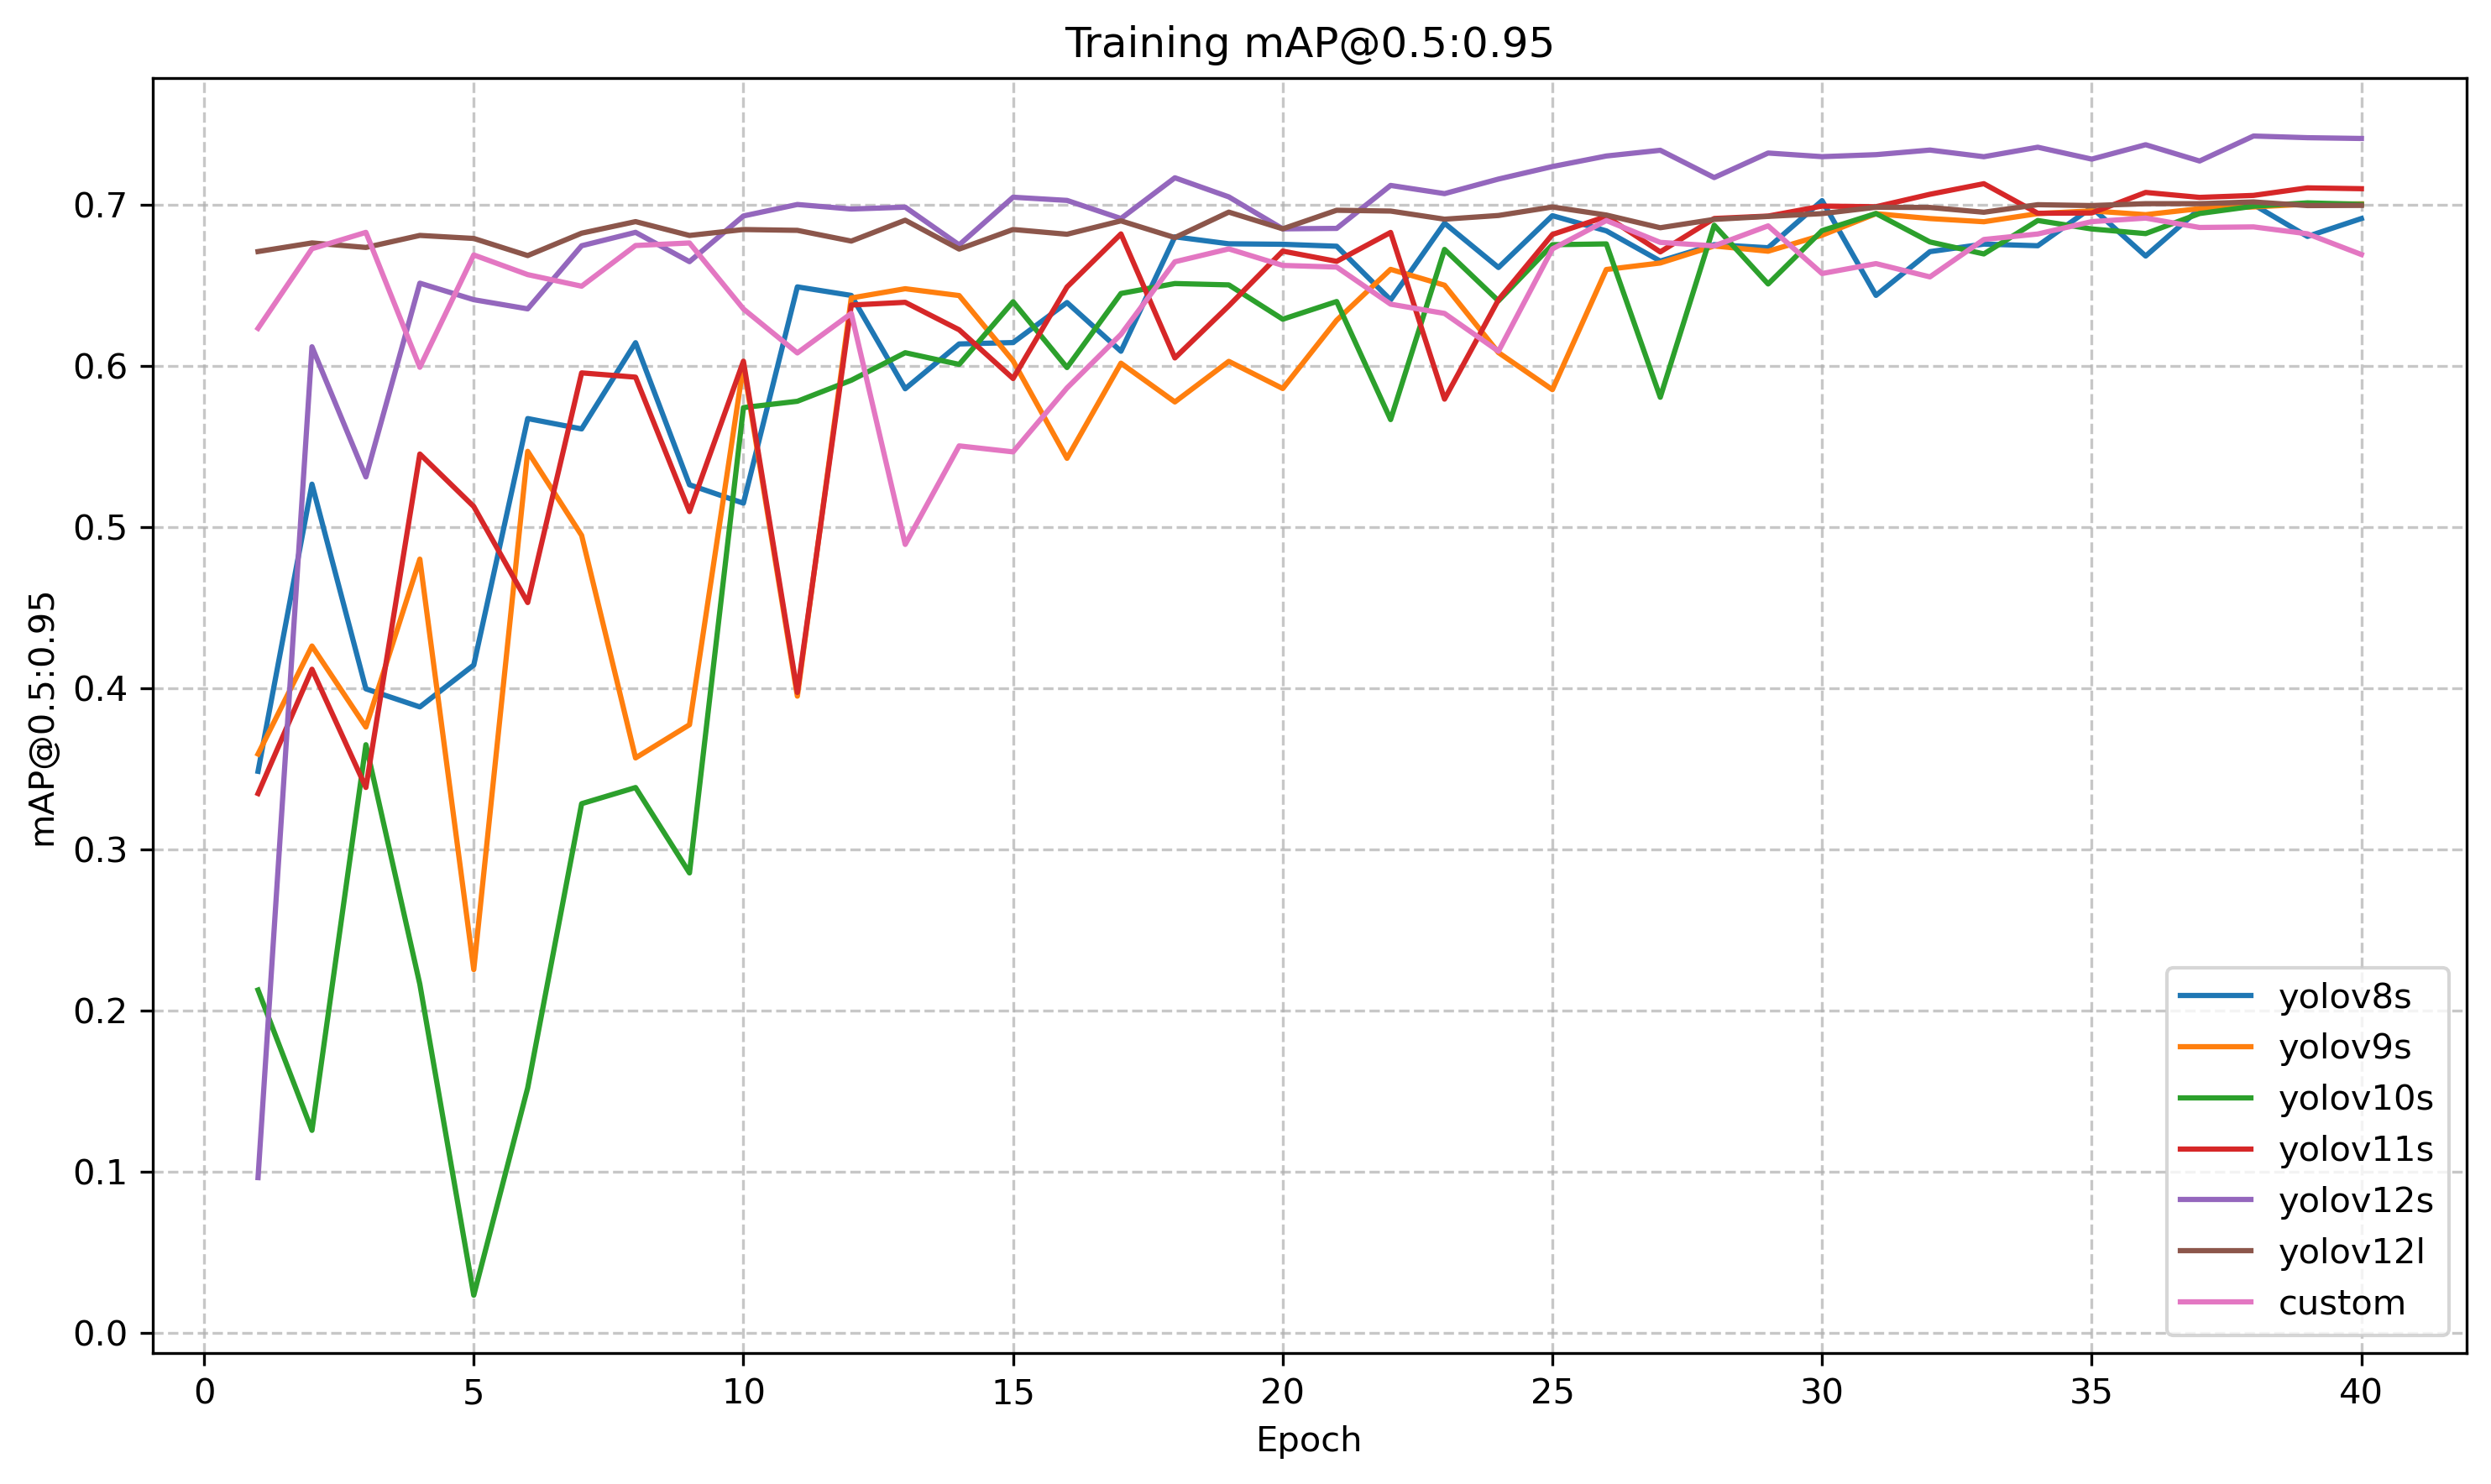
\includegraphics[width=1.0\textwidth]{figuras/YOLO_plots/map50-95.png}
  \caption{mAP@0.5:0.95 durante el proceso de entrenamiento.}
  \label{fig:yolo_train_map95}
\end{figure}

\begin{figure}[H]
  \centering
  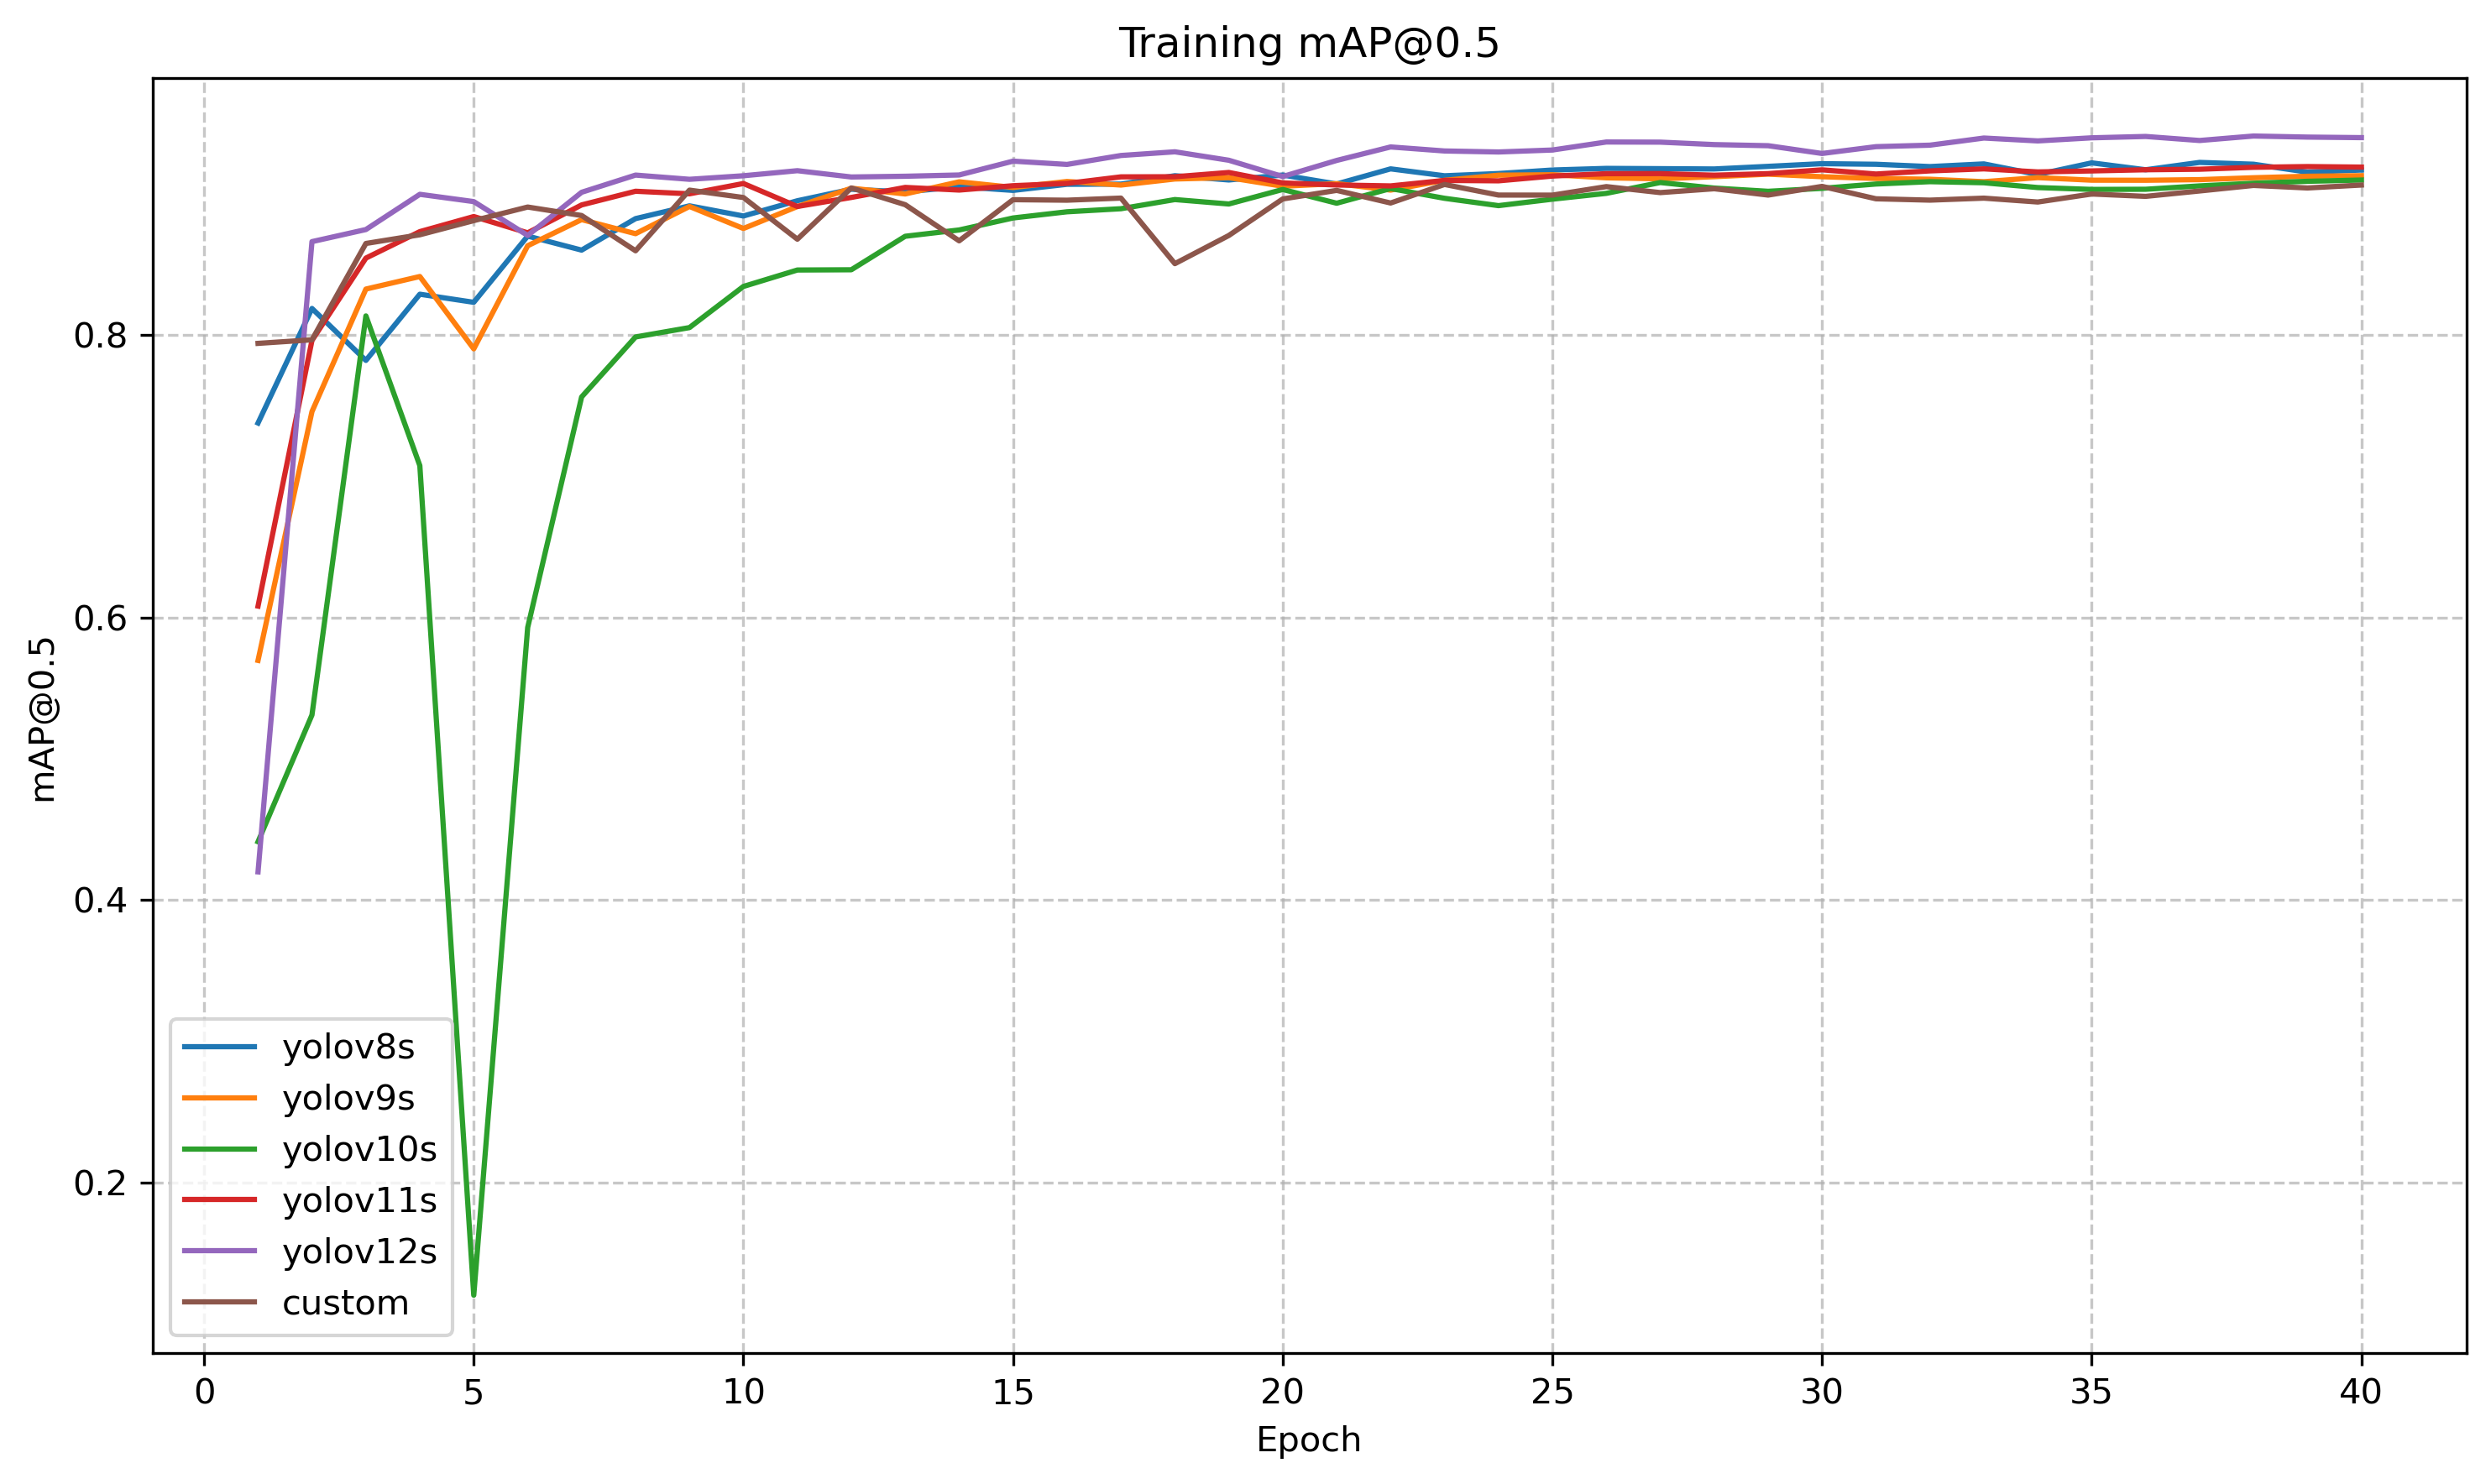
\includegraphics[width=1.0\textwidth]{figuras/YOLO_plots/map50.png}
  \caption{mAP@0.5 durante el proceso de entrenamiento.}
  \label{fig:yolo_train_map50}
\end{figure}

\begin{figure}[H]
  \centering
  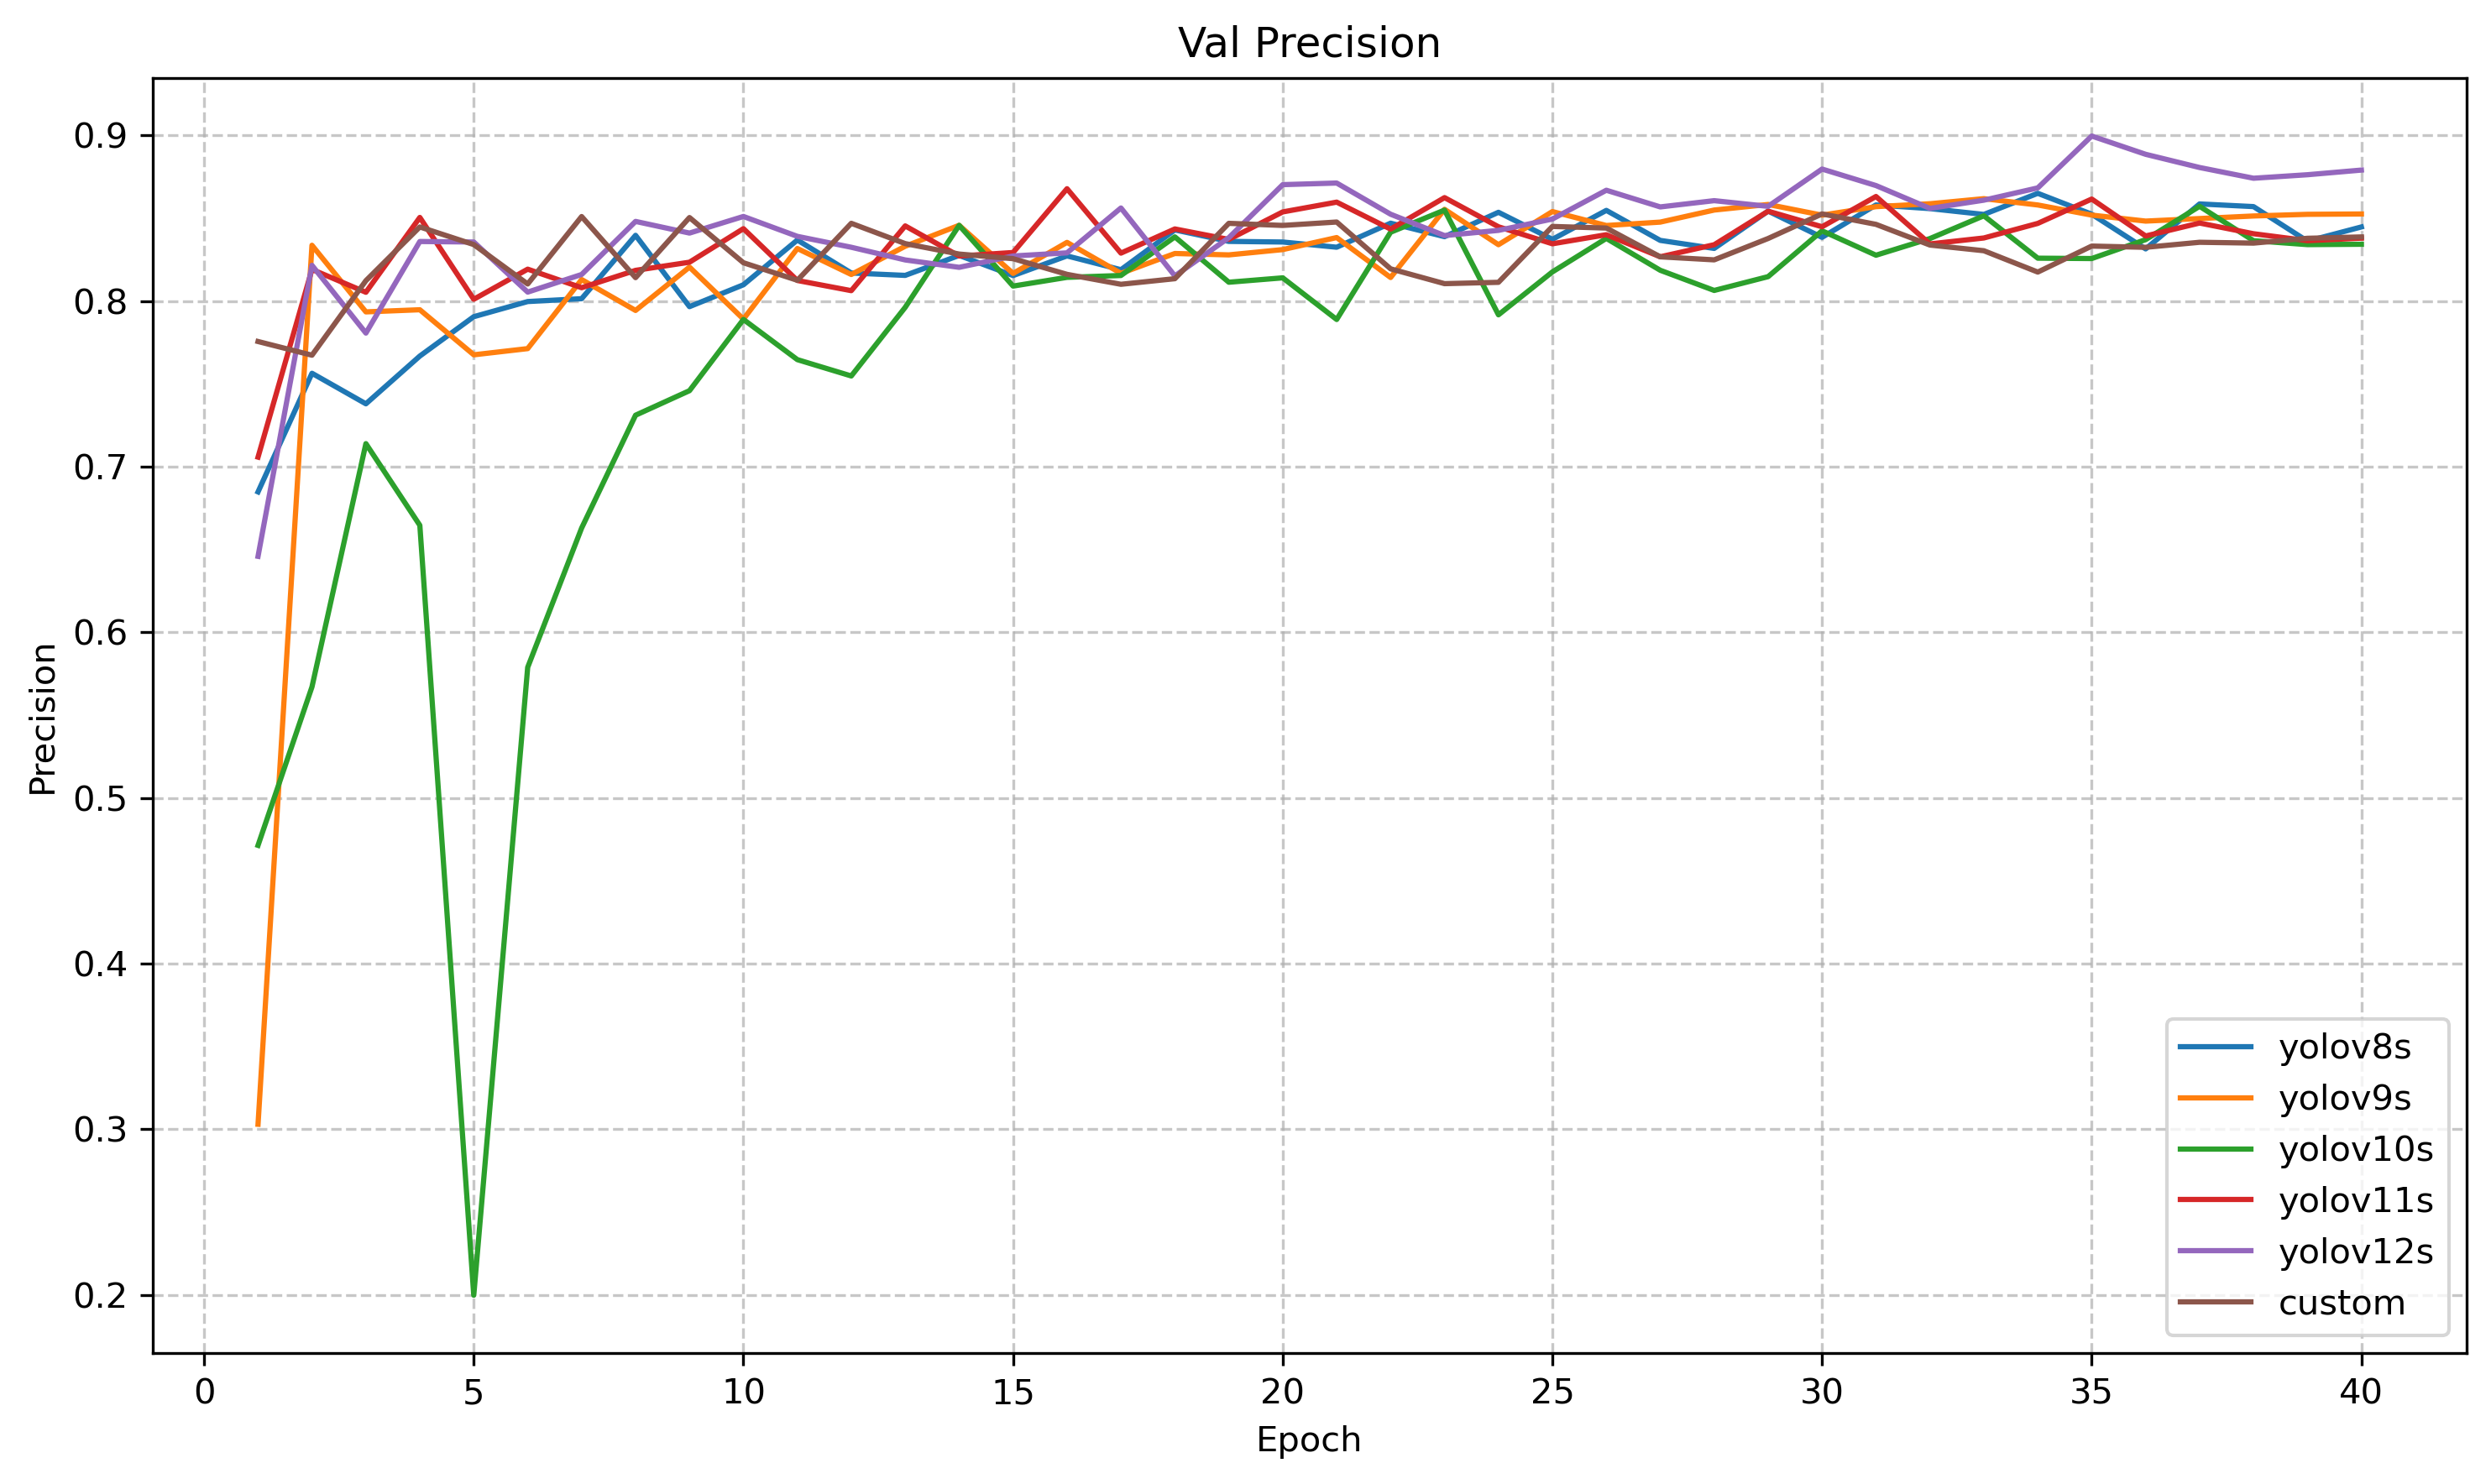
\includegraphics[width=1.0\textwidth]{figuras/yolo_plots/precision.png}
  \caption{\textit{Precision} del modelo sobre el conjunto de validación.}
  \label{fig:yolo_train_precision}
\end{figure}

\begin{figure}[H]
  \centering
  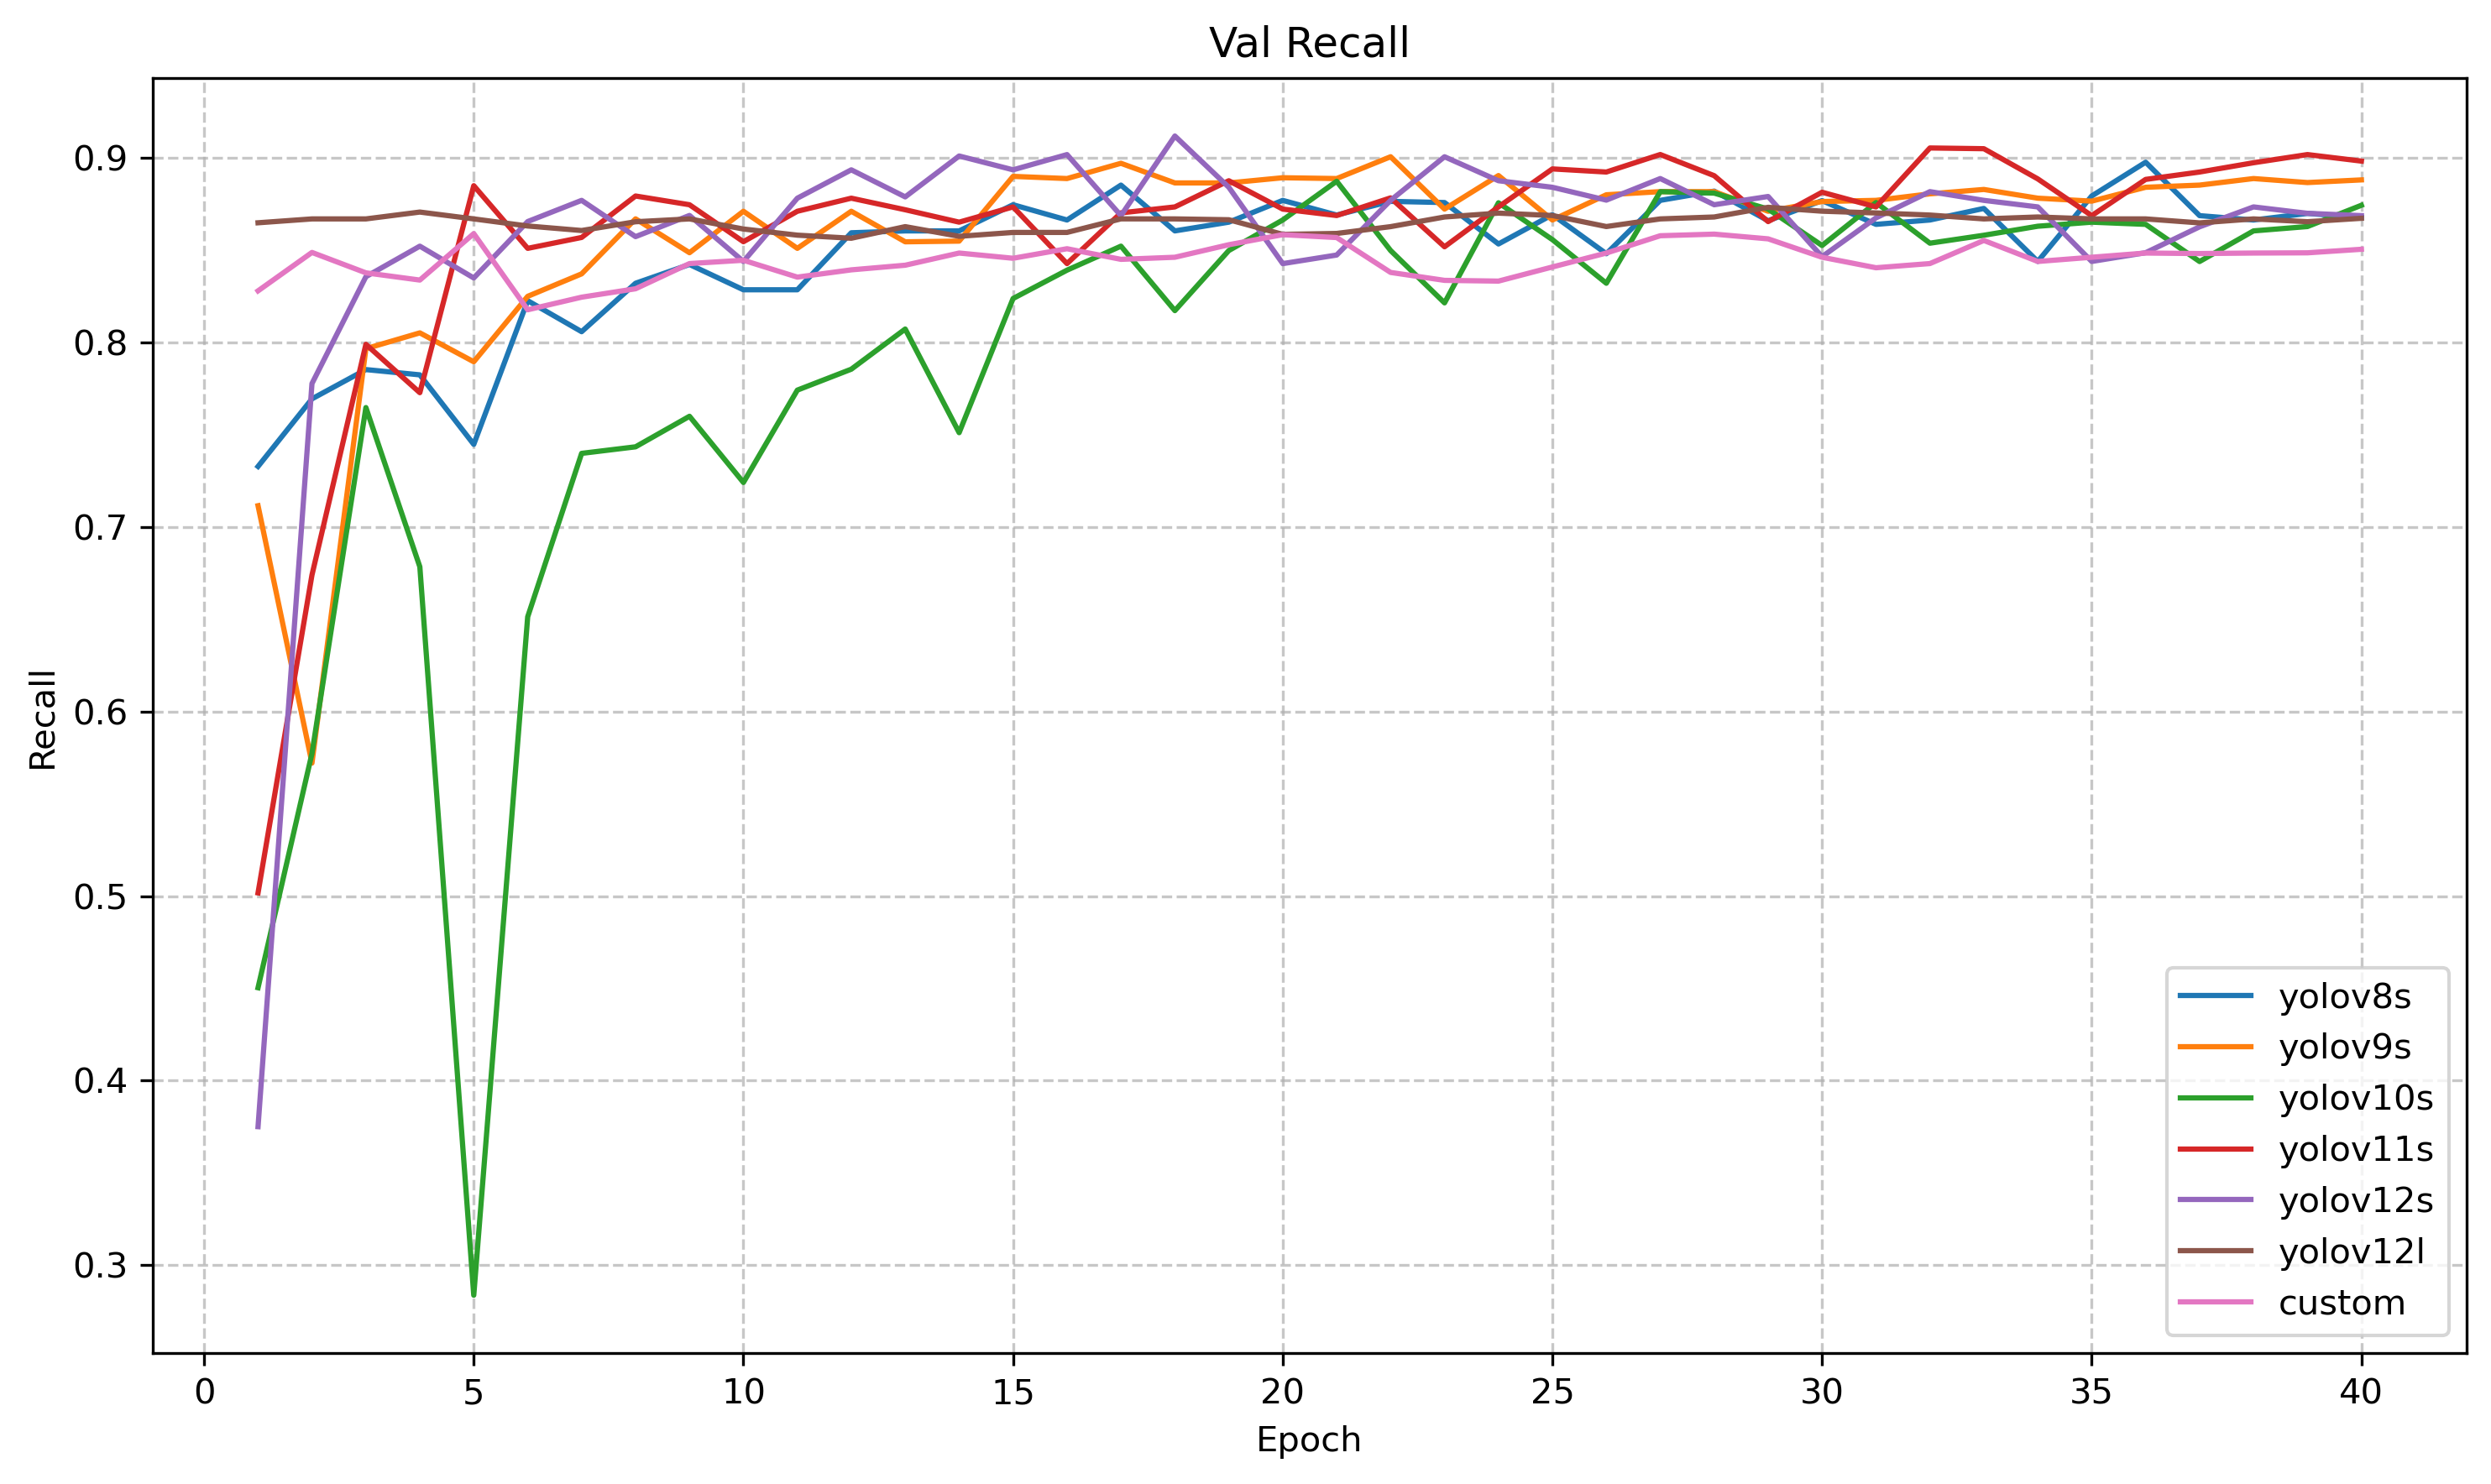
\includegraphics[width=1.0\textwidth]{figuras/yolo_plots/recall.png}
  \caption{\textit{Recall} del modelo sobre el conjunto de validación.}
  \label{fig:yolo_train_recall}
\end{figure}

\begin{figure}[H]
  \centering
  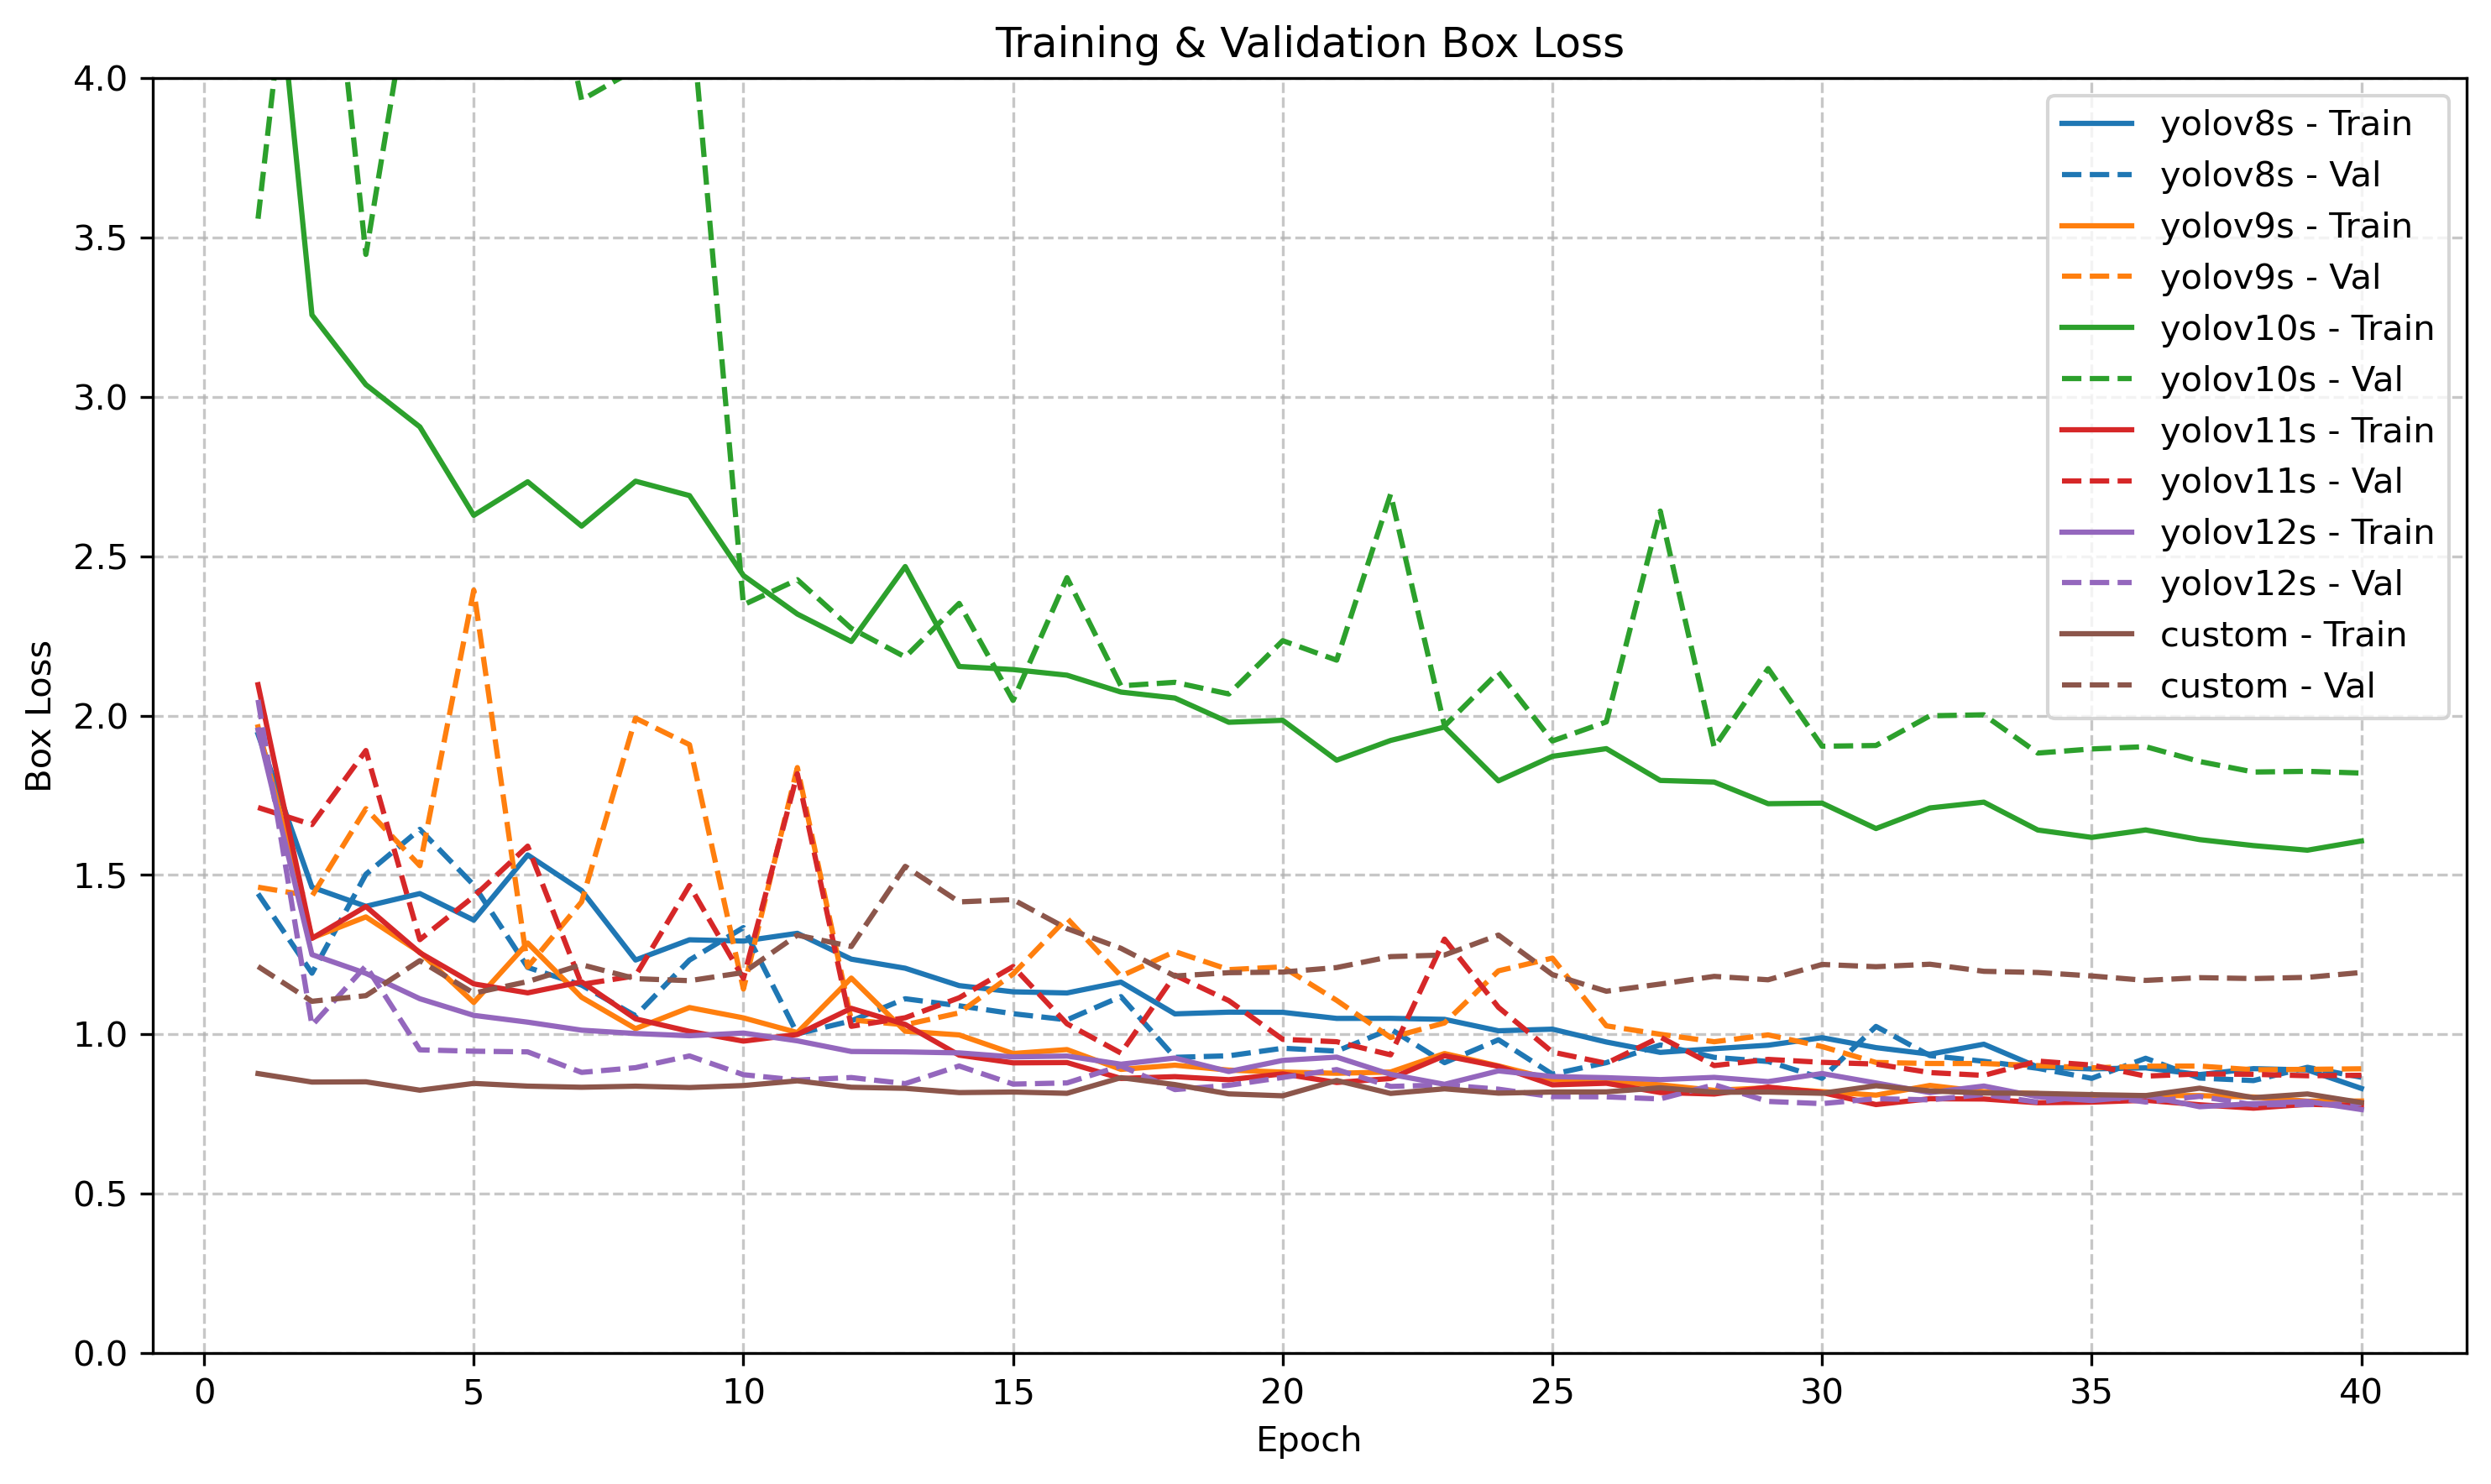
\includegraphics[width=1.0\textwidth]{figuras/yolo_plots/box_loss.png}
  \caption{\textit{Box Loss} sobre el conjunto de entrenamiento y validación.}
  \label{fig:yolo_train_box_loss}
\end{figure}

\begin{figure}[H]
  \centering
  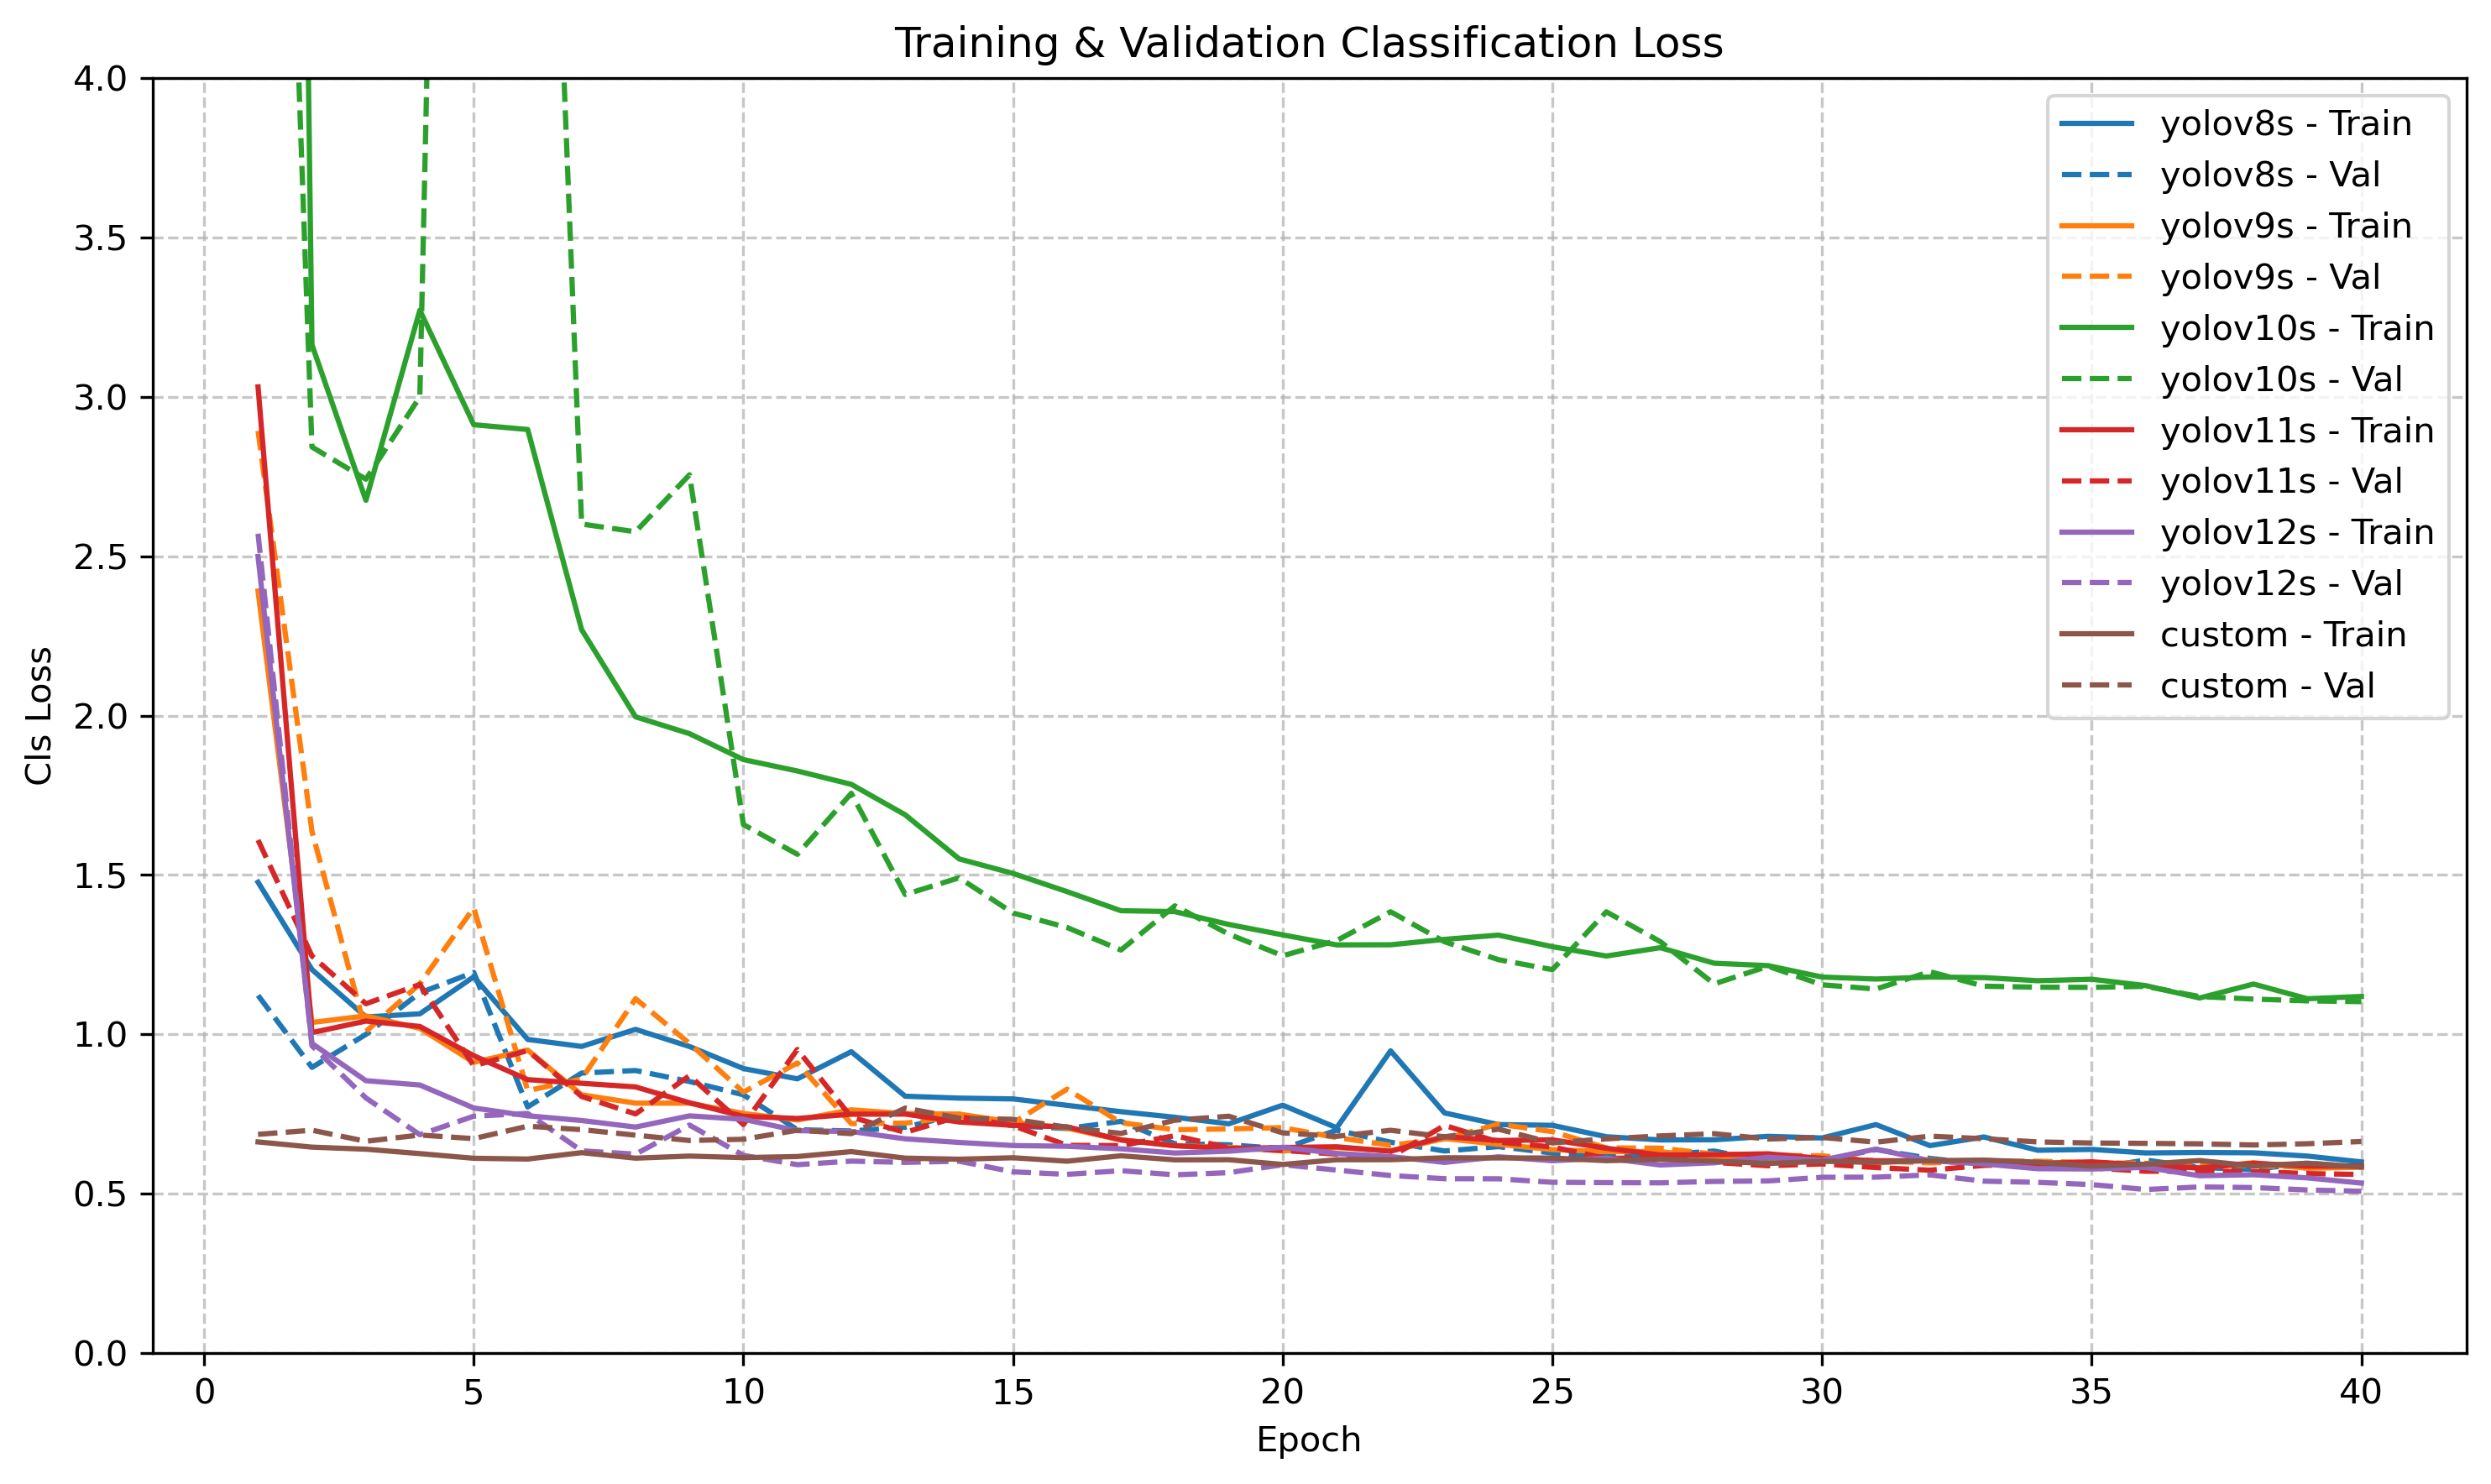
\includegraphics[width=1.0\textwidth]{figuras/yolo_plots/cls_loss.png}
  \caption{\textit{Classification Loss} sobre el conjunto de entrenamiento y validación.}
  \label{fig:yolo_train_cls_loss}
\end{figure}

En general, todos los modelos muestran un buen desempeño durante el entrenamiento, con métricas que mejoran y se estabilizan a lo largo de las 40 épocas (\textit{epoch}). Además, 
no hay evidencia de un sobreajuste (\textit{overfitting}).

Aparentemente el modelo YOLOv12s arroja mejores resultados; principalmente, en la métrica más exigente, la mAP@0.5:0.95 (\autoref{fig:yolo_train_map95}). En base a esta métrica, el peor modelo se puede considerar el \textit{custom}.
Sorprendentemente, el modelo YOLOv12l (el más grande y preciso) es el peor modelo en cuanto a las métricas mAP@0.5 (\autoref{fig:yolo_train_map50}) y \textit{precision} sobre el conjunto de validación (\autoref{fig:yolo_train_precision}). 

Los buenos rendimientos del modelo YOLOv10s en las métricas de \textit{precision, recall y mAP}, se aprecia que la función de pérdida (\textit{loss}), tanto en la clasificación como en las \textit{bounding boxes},
el modelo se distancia respecto al resto con una pérdida superior a la de los demás. No es una pérdida muy significativa, es importante tenerla en cuenta, por ser la métrica a minimizar durante el entrenamiento.
Se puede ver que, en las primeras épocas, al modelo le cuesta mucho aprender a localizar y clasificar los objetos correctamente, aunque finalmente consigue estabilizarse.

\subsection{Validación cruzada}
\label{sec:Validación cruzada}

Para demostrar la capacidad de generalización y fiabilidad de los diferentes modelos de detección de células redondas, se emplea la metodología
de validación cruzada (\textit{k-fold cross validation}). Para ello, se ha dividido el conjunto de entrenamiento original constituido por 373 imágenes (\autoref{tab:dataset_original}) en $k=4$ pliegues o \textit{folds} de tamaño similar.
De este modo, el proceso de entrenamiento tiene lugar con las 4 combinaciones (sin repetición) posibles, en las que un \textit{fold} se reserva para validar y tres para entrenar. Los resultados promediados obtenidos para cada modelo se recogen en la \autoref{tab:kfold_resultados}.

\section{Métricas}
\label{sec:Métricas}
Para la evaluación de los modelos, se emplea un conjunto de métricas fundamentales que se exponen a continuación.

\begin{description}
  \item[\textit{Precision}]: Mide la proporción de detecciones correctas entre todas las detecciones realizadas:
  \[
    \mathrm{\textit{Precision}} = \frac{TP}{TP + FP}
  \]
  donde TP son los verdaderos positivos (considerando la clase positiva como célula redonda) y FP los falsos positivos. Alta \textit{precision} indica pocas detecciones de células redondas 
  que no se corresponden con una célula redonda real.

  \item[\textit{Recall}]: Mide la proporción de instancias reales que han sido detectadas:
  \[
    \mathrm{\textit{Recall}} = \frac{TP}{TP + FN}
  \]
  donde FN son los falsos negativos. Un \textit{recall} alto indica que el modelo encuentra la mayoría de las instancias reales.

  \item[\textit{F1-score}]: Es la media armónica entre la precisión y el \textit{recall}, proporcionando una medida única que equilibra ambos aspectos. Se calcula como:
  \[
    \mathrm{F1} = 2 \cdot \frac{\mathrm{Precision} \cdot \mathrm{Recall}}{\mathrm{Precision} + \mathrm{Recall}}
  \]
  El \textit{F1-score} es especialmente útil cuando es importante considerar tanto los falsos positivos como los falsos negativos. En este trabajo se utiliza como métrica principal en las curvas F1-confianza y en la herramienta web.

  \item[\textit{mean Average Precision (mAP)}]: Para detección de objetos se calcula la curva \textit{precision}–\textit{recall} para cada clase y su área bajo la curva (AP). El \textit{mean Average Precision} es la media de las AP sobre todas las clases:
  \[
    \mathrm{mAP} = \frac{1}{C}\sum_{c=1}^{C} \mathrm{AP}_c
  \]
  donde $C$ es el número de clases. En detección se considera una predicción como verdadero positivo si el \textit{Intersection over Union} (IoU) entre la caja predicha y la caja \textit{ground truth} supera un umbral (por ejemplo IoU $\geq 0.5$). 

  \medskip

  \noindent\textbf{mAP@0.5 (mAP50):} Es la mAP calculada usando un único umbral de IoU igual a 0.5. Formalmente:
  \[
    \mathrm{mAP@0.5} \;=\; \frac{1}{C}\sum_{c=1}^{C} \mathrm{AP}_c(\mathrm{IoU}=0.5)
  \]
  Es una medida menos exigente, que acepta solapamientos moderados entre predicción y \textit{ground truth}.

  \medskip

  \noindent\textbf{mAP@[0.5:0.95] (mAP50:95):} Es la mAP estándar del \textit{benchmark} COCO que promedia la AP de cada clase sobre múltiples umbrales de IoU desde 0.50 hasta 0.95 con paso 0.05 (10 umbrales: 0.50, 0.55, …, 0.95). Nota: COCO calcula cada AP integrando la curva \textit{precision}–\textit{recall} muestreada en 101 puntos, y después se promedian las AP en los 10 umbrales para obtener mAP@[0.5:0.95].
  \[
    \mathrm{mAP}_{[0.5:0.95]} \;=\; \frac{1}{C}\frac{1}{T}\sum_{c=1}^{C}\sum_{t\in\{0.50,0.55,\dots,0.95\}} \mathrm{AP}_c(\mathrm{IoU}=t)
  \]
  donde $T=10$. Esta métrica es más exigente porque penaliza detecciones con IoU bajos y refleja mejor la precisión espacial del modelo.

  \item[Inferencia (ms)] Tiempo medio (en milisegundos) que tarda un modelo en evaluar una única imagen (inferencia). Relevante para proyectos en tiempo real.

\end{description}
\arrayrulecolor[HTML]{B9DAE1}


\chapter{Resultados} %%%%%%%%%%%%%%%%%%%%%%%%%%%%%%%%%%%%%%%%%%%%%%%%%%%%%%%
\label{Resultados}

En este capítulo se abordan los resultados obtenidos para los modelos sobre los diferentes conjuntos de \textit{test}. Para esto, se analizan 
los resultados atendiendo a dos enfoques complementarios: 
por un lado, se presentan los resultados cuantitativos, basados en métricas objetivas de evaluación; y por otro, se realiza un análisis cualitativo, 
centrado en la interpretación visual y contextual de las predicciones realizadas por los modelos.

\section{Validación cruzada}
\label{sec:Validación cruzada}

Los resultados obtenidos mediante la validación cruzada (\textit{k-fold}) se presentan en la \autoref{tab:kfold_resultados}.

\begin{table}[htbp]
\caption{Resultados de la validación cruzada (\textit{k-fold}) para todos los modelos}
\label{tab:kfold_resultados}
\centering
\begin{tabular}{lcccc}
\toprule
\textbf{Modelo} & \textbf{\textit{Precision}} & \textbf{\textit{Recall}} & \textbf{mAP50} & \textbf{mAP50-95} \\
\midrule
YOLOv8s  & 0,836 $\pm$ 0,008 & 0,868 $\pm$ 0,015 & 0,914 $\pm$ 0,011 & 0,723 $\pm$ 0,024 \\
YOLOv9s  & 0,852 $\pm$ 0,015 & 0,866 $\pm$ 0,013 & 0,919 $\pm$ 0,009 & 0,729 $\pm$ 0,026 \\
YOLOv10s & 0,854 $\pm$ 0,014 & 0,855 $\pm$ 0,011 & 0,918 $\pm$ 0,009 & 0,739 $\pm$ 0,029 \\
YOLOv11s & 0,845 $\pm$ 0,025 & \textbf{0,869 $\pm$ 0,013} & \textbf{0,922 $\pm$ 0,012} & \textbf{0,742 $\pm$ 0,025} \\
YOLOv12s & \textbf{0,853 $\pm$ 0,011} & 0,861 $\pm$ 0,016 & 0,918 $\pm$ 0,008 & 0,730 $\pm$ 0,018 \\
YOLOv12l & 0,841 $\pm$ 0,002 & 0,867 $\pm$ 0,013 & 0,912 $\pm$ 0,011 & 0,724 $\pm$ 0,013 \\
\textit{custom}   & 0,836 $\pm$ 0,014 & 0,865 $\pm$ 0,014 & 0,905 $\pm$ 0,011 & 0,707 $\pm$ 0,015 \\
\bottomrule
\end{tabular}
\end{table}

Los datos de la \autoref{tab:kfold_resultados} se representan en la \autoref{fig:yolo_k-fold}.
En esta figura, cada punto central indica el valor medio de rendimiento para una métrica específica (\textit{precision}, \textit{recall}, mAP50 y mAP50-95), 
mientras que las barras horizontales que lo rodean representan la desviación estándar obtenida a lo largo de los 4 pliegues de la validación cruzada.

Analizando la \autoref{fig:yolo_k-fold}, se puede observar que, pese a las pequeñas diferencias en los promedios, los intervalos de incertidumbre se solapan entre todos los modelos
para todas las métricas específicas a evaluar. Es un claro indicador de que los modelos ofrecen un rendimiento similar y robusto, que les permite generalizar de forma adecuada, pese al despunte del modelo YOLOv11s. 
Asimismo, las barras de incertidumbre más pequeñas reflejan qué modelos son más estables, destacando los modelos YOLOv12s, YOLOv12l y \textit{custom}.

De este modo, la elección de un único "mejor" modelo es difícil, ya que son todos ellos opciones excelentes y estadísticamente equivalentes para esta tarea de detección de objetos. 

\begin{figure}[H]
  \centering
  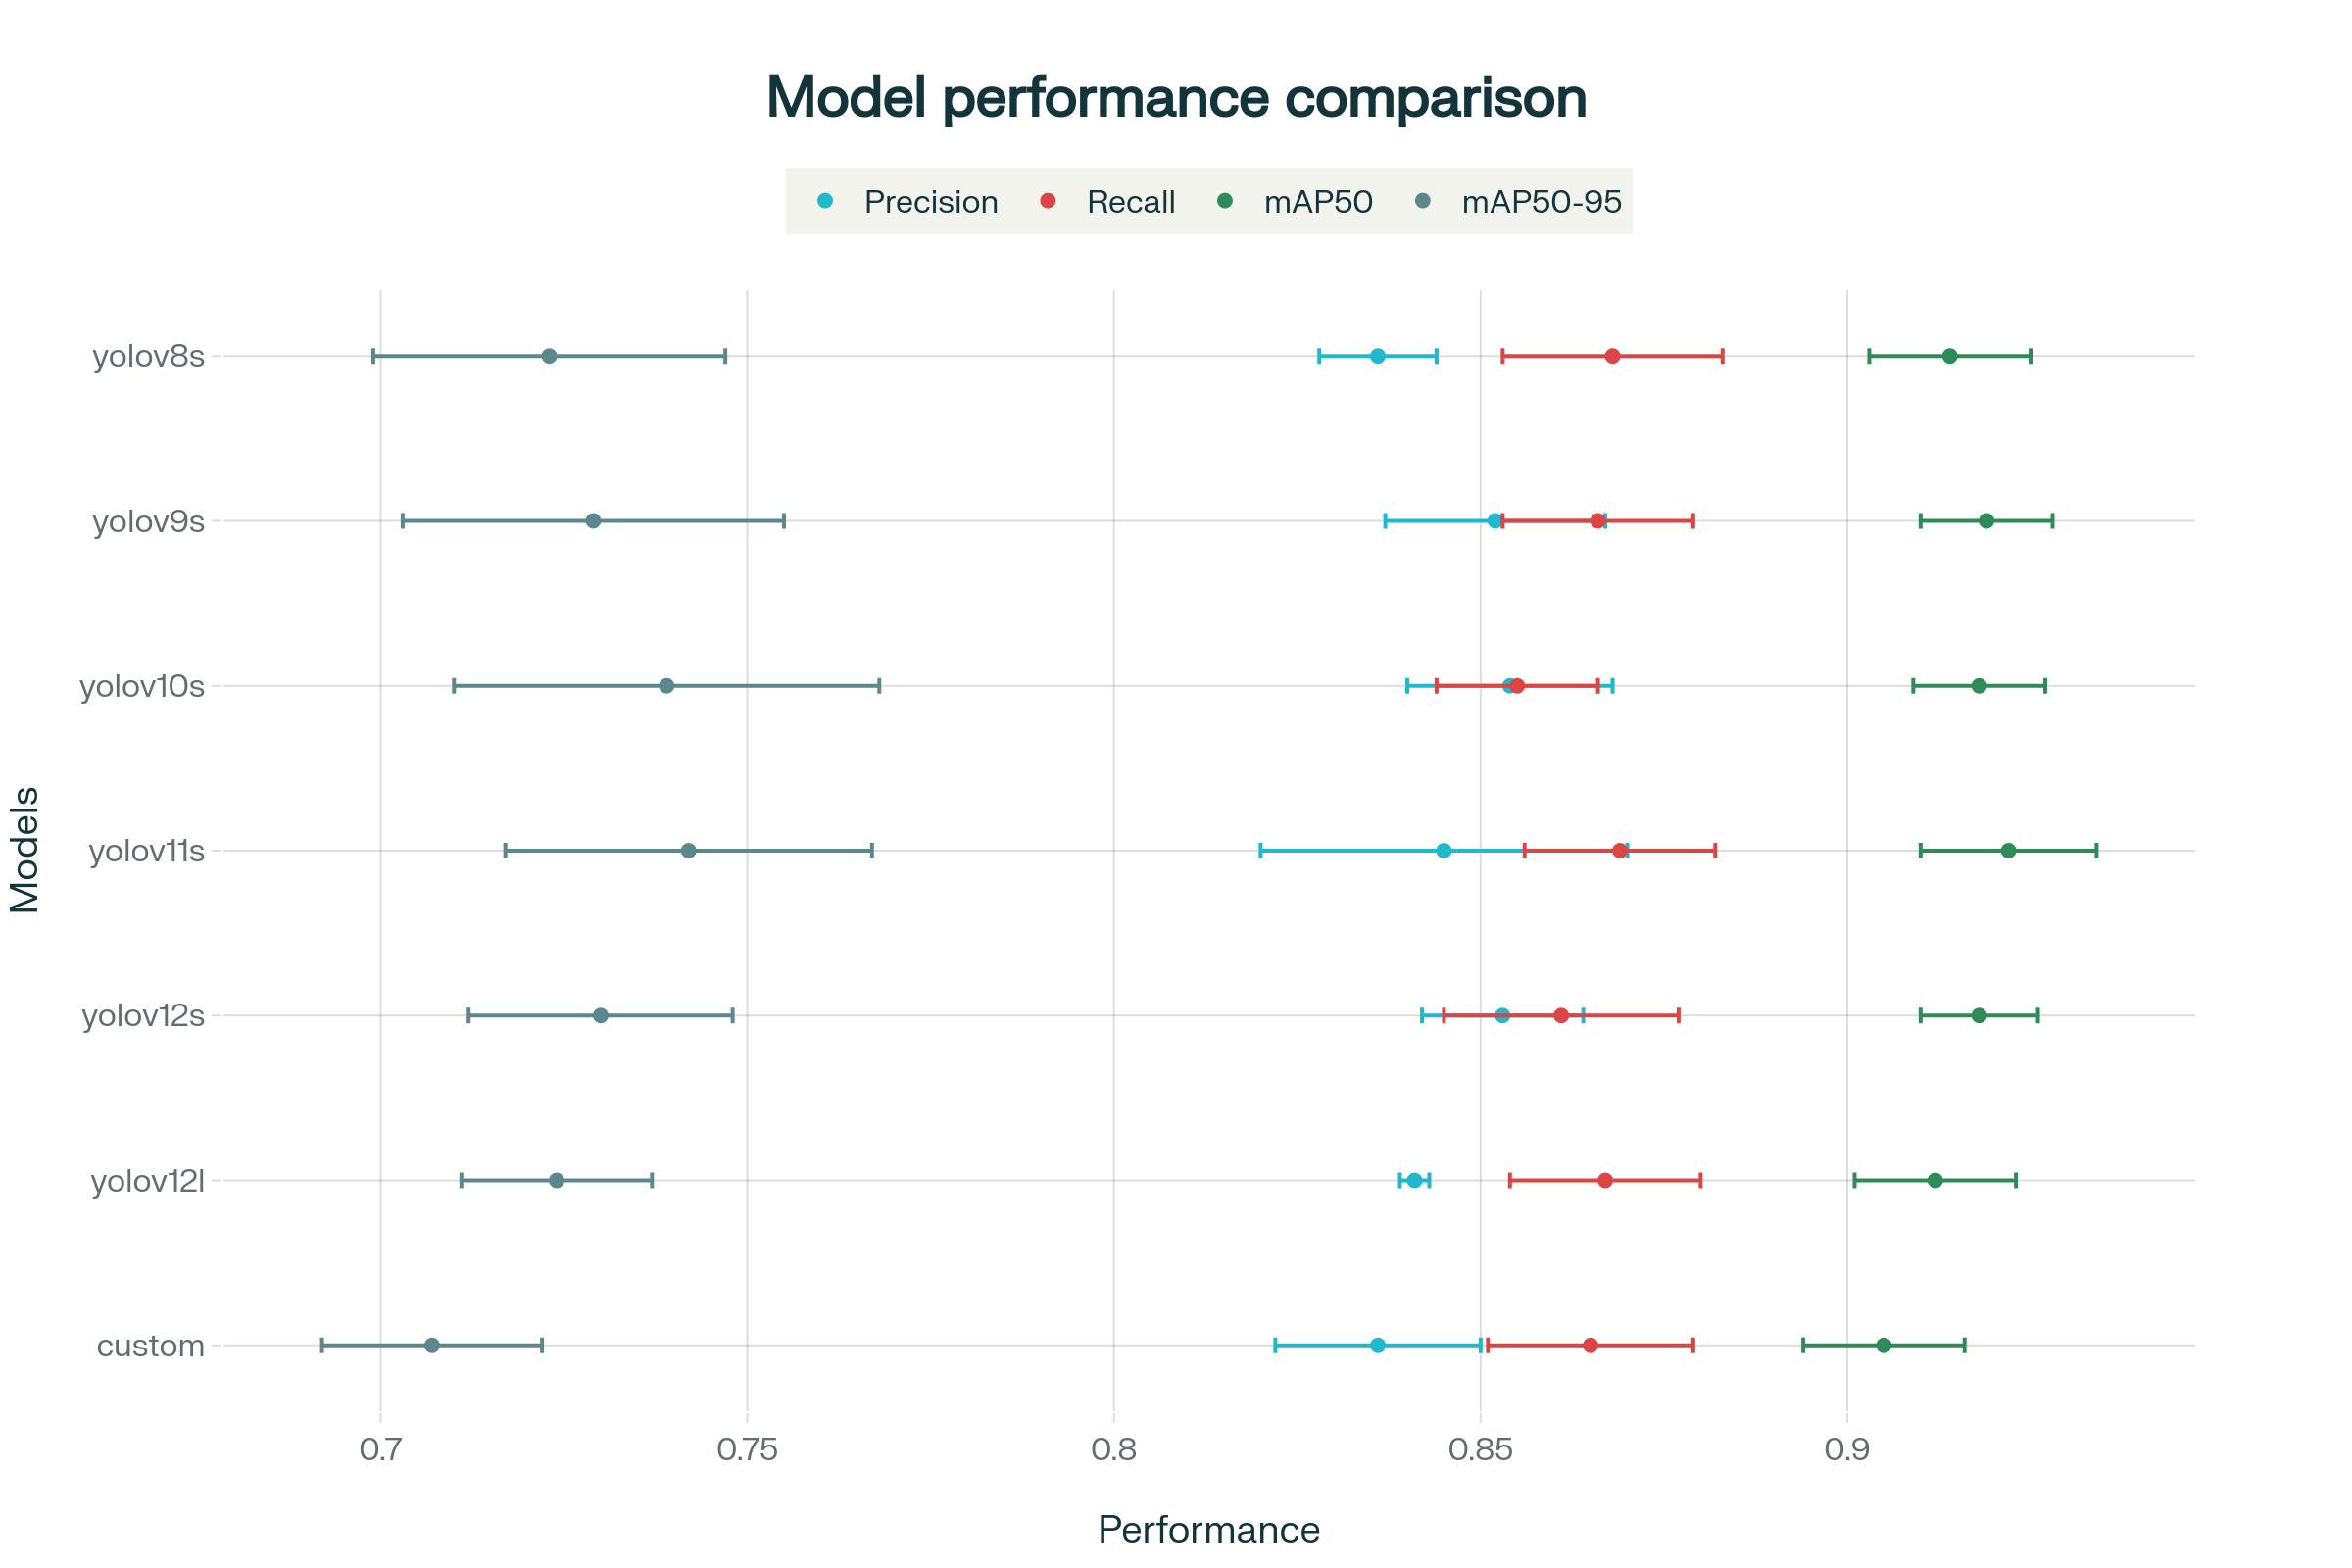
\includegraphics[width=1.0\textwidth]{figuras/k-fold/Yolo_k-fold.png}
  \caption{Resultados obtenidos mediante validación cruzada (k-fold).}
  \label{fig:yolo_k-fold}
\end{figure}

\section{Resultados cuantitativos}
\label{sec:Resultados cuantitativos}

En esta primera parte, se evalúan los resultados sobre el conjunto de \textit{test} original para el cual se tienen resultados asociados
a la PoC previa (\autoref{tab:yolov7_results}), bajo la premisa de que todos los modelos arrojan resultados similares, por los tiempos de inferencia y 
el valor más alto en la métrica mAP@0.5:0.95, el mejor modelo es YOLOv7.

\begin{table}[H]
  \caption{Resultados de los modelos en la prueba de concepto inicial \cite{HamiltonThorneRoundCells}}
  \centering
  \resizebox{\textwidth}{!}{
  \begin{tabular}{lccccc}
      \hline
      \textbf{Modelo} & \textbf{Precisión (P)} & \textbf{\textit{recall} (R)} & \textbf{mAP@0.5} & \textbf{mAP@0.5:0.95} & \textbf{Inferencia (ms)} \\
      \hline
      YOLOv7      & 0,870  & \textbf{0,889} & \textbf{0,935} & \textbf{0,722} & 20,0   \\
      YOLOv7-W6   & 0,847 & 0,883 & 0,925 & 0,694 & \textbf{16,0}   \\
      YOLOv7-E6E  & \textbf{0,906} & 0,857 & 0,934 & 0,721 & 127,5  \\
      \hline
  \end{tabular}
  }
  \label{tab:yolov7_results}
\end{table}

\begin{table}[H]
  \caption{Resultados de los modelos sobre el conjunto de \textit{test} original}
  \centering
  \resizebox{\textwidth}{!}{
  \begin{tabular}{lccccc}
      \hline
      \textbf{Modelo} & \textbf{Precisión (P)} & \textbf{\textit{recall} (R)} & \textbf{mAP@0.5} & \textbf{mAP@0.5:0.95} & \textbf{Inferencia (ms)} \\
      \hline
      YOLOv8s    & 0,843 & 0,844 & 0,920 & 0,722 & \textbf{11,006} \\
      YOLOv9s    & 0,838 & 0,852 & 0,921 & 0,721 & 13,485 \\
      YOLOv10s   & 0,821 & 0,867 & 0,918 & 0,717 & 11,221 \\
      YOLOv11s   & \textbf{0,861} & 0,824 & 0,921 & 0,732 & 11,248 \\
      YOLOv12s   & 0,856 & 0,863 & \textbf{0,936} & \textbf{0,760} & 14,615 \\
      YOLOv12l   & 0,856 & 0,836 & 0,921 & 0,729 & 48,146 \\
      \textit{custom}     & 0,835 & 0,838 & 0,909 & 0,695 & 13,058 \\
      \textit{ensemble}   & 0,815 & \textbf{0,895} & 0,864 & 0,697 & 75,073 \\
      \hline
  \end{tabular}
  }
  \label{tab:yolov8_12_results}
\end{table}

Comparando los resultados de la POC con los obtenidos en este proyecto (\autoref{tab:yolov8_12_results}), el modelo YOLOv12s destaca por mejorar las métricas mAP@0.5 y mAP@0.5:0.95 (un $0,10\%$ y $5.26\%$, respectivamente, respecto a YOLOv7, el mejor modelo de la PoC anterior) y 
reducir la latencia ($5,4$ ms), por lo que se considera el mejor modelo en esta prueba. Aunque los modelos más pesados como YOLOv12l y el ensamblado 
presentan mayores tiempos de inferencia, todos los modelos mantienen una latencia inferior a 100 ms, un tiempo de respuesta excelente para una herramienta de uso clínico. 

Si el objetivo es no pasar por alto ninguna célula redonda, el modelo \textit{ensemble} es la mejor opción, ya que alcanza el \textit{recall} más alto (0,895),
aunque a costa de una menor \textit{precision} (0,815) y mAP@0.5 (0,864). Si se busca rapidez sin sacrificar demasiado el rendimiento, el modelo YOLOv8 es el indicado. Con un tiempo de inferencia de tan solo 11.006 ms, es el más rápido de todos.
Cuando la prioridad es la confianza en cada detección, YOLOv11s destaca al obtener la mayor precisión (0,861), aunque con el \textit{recall} más bajo (0,824).

Analizando los nuevos conjuntos de \textit{test} (\autoref{tab:yolos_nuevos_tests}), los resultados siguen siendo similares entre modelos. Según la métrica mAP@0.5:0.95, YOLOv12s vuelve a ser el mejor (0.673), seguido de YOLOv12l (0.659). 
El \textit{ensemble} mejora precisión y \textit{recall}, pero empeora mAP y latencia. El modelo \textit{custom} destaca por su baja latencia y buenos resultados, especialmente en test3, 
donde iguala la precisión del \textit{ensemble} ($0.873$). Las diferencias entre el resto de modelos son mínimas.

Tras el proceso de reetiquetado del conjunto de \textit{test} original, es decir, en la evaluación sobre el conjunto de test, se observan cambios interesantes que 
sugieren una mejora en la calidad del \textit{ground truth} (mejora la sensibilidad de la detección). La mayoría de los modelos muestran una mejora en la \textit{precision}, destaca el modelo \textit{ensemble} con el mayor incremento (+0,054). 
En cuanto al \textit{recall}, los resultados son más variados, pero YOLOv12l y YOLOv11s muestran mejoras significativas.
La métrica mAP@0.5 mejora en la mayoría de los modelos mientras que la métrica mAP@0.5:0.95 sufre un descenso generalizado. Esto sugiere que, si bien los modelos identifican mejor las células redondas, la precisión de las \textit{bounding boxes} ha disminuido ligeramente.
Asimismo, los tiempos de inferencia se mantienen con variaciones mínimas en la mayoría de los modelos.

El conjunto test2 muestra latencias más altas ($31$–$76$ ms) y un descenso general de mAP@0.5:0.95, lo que indica condiciones diferentes que afectan al rendimiento. 
Esto tiene sentido pues cada test contiene imágenes con diferentes grados de patología.

En resumen, YOLOv12s es el modelo más destacado entre las arquitecturas evaluadas. El ensamblado de modelos mejora \textit{recall} y precisión al reducir falsos negativos, aunque aumenta los falsos positivos, como muestran las matrices de confusión 
(\autoref{sec:Matrice de confusión}). En test2, las diferencias son mínimas debido al tamaño reducido del conjunto. El análisis de las curvas F1-confianza 
(\autoref{sec:Curvas F1-confianza}) indica que el \textit{F1-score} óptimo se alcanza con umbrales de confianza entre 0.25 y 0.5, por lo que se estudia YOLOv12s con un umbral de 0.35 
para imágenes de alta resolución.

% Tabla para los resultados sobre los conjuntos de Test
\definecolor{turquoise}{RGB}{64,224,208}
\begin{table}[ht]
\caption{Evaluación de modelos sobre los nuevos conjuntos de \textit{test}}
\centering
\rowcolors{2}{gray!15}{white}
\renewcommand{\arraystretch}{1.3}
\setlength{\arrayrulewidth}{1.2pt}
\resizebox{\textwidth}{!}{
\arrayrulecolor{gray}
\begin{tabular}{!{\vrule width 1.2pt}l|c|c|c|c|c|c!{\vrule width 1.2pt}}
\arrayrulecolor{black}
\specialrule{1.5pt}{0pt}{0pt}
\rowcolor{gray!30}
\textbf{Modelo} & \textbf{Test} & \textbf{Precisión} & \textbf{Recall} & \textbf{mAP@0.5} & \textbf{mAP@0.5:0.95} & \textbf{Inferencia (ms)} \\
\specialrule{1.2pt}{0pt}{0pt}
\arrayrulecolor{gray}
YOLOv8s   & test  & 0,855 & 0,838 & 0,926 & 0,704 & 11,844 \\ \hline
YOLOv9s   & test  & 0,851 & 0,876 & 0,933 & 0,706 & 13,492 \\ \hline
YOLOv10s  & test  & 0,851 & 0,862 & 0,927 & 0,701 & \cellcolor{turquoise!30}\textbf{11,120} \\ \hline
YOLOv11s  & test  & 0,846 & 0,866 & 0,930 & 0,716 & 12,143 \\ \hline
YOLOv12s  & test  & 0,862 & 0,848 & \cellcolor{turquoise!30}\textbf{0,936} & \cellcolor{turquoise!30}\textbf{0,740} & 14,519 \\ \hline
YOLOv12l  & test  & 0,846 & \cellcolor{turquoise!30}\textbf{0,889} & 0,934 & 0,714 & 45,214 \\ \hline
\textit{custom}    & test  & 0,845 & 0,853 & 0,919 & 0,678 & 12,913 \\ \hline
\textit{ensemble} & test & \cellcolor{turquoise!30}\textbf{0,869} & 0,860 & 0,842 & 0,664 & 69,572 \\
\arrayrulecolor{black}
\specialrule{1.2pt}{0pt}{0pt}
\arrayrulecolor{gray}
YOLOv8s   & test2 & 0,924 & 0,938 & 0,969 & 0,553 & \cellcolor{turquoise!30}\textbf{30,901} \\ \hline
YOLOv9s   & test2 & 0,917 & 0,927 & 0,961 & 0,542 & 46,502 \\ \hline
YOLOv10s  & test2 & 0,956 & 0,898 & 0,962 & \cellcolor{turquoise!30}\textbf{0,589} & 34,355 \\ \hline
YOLOv11s  & test2 & 0,929 & 0,917 & 0,964 & 0,534 & 33,114 \\ \hline
YOLOv12s  & test2 & \cellcolor{turquoise!30}\textbf{0,965} & 0,917 & \cellcolor{turquoise!30}\textbf{0,975} & 0,556 & 51,508 \\ \hline
YOLOv12l  & test2 & 0,957 & 0,926 & \cellcolor{turquoise!30}\textbf{0,975} & 0,562 & 75,871 \\ \hline
\textit{custom}    & test2 & 0,945 & 0,903 & 0,957 & 0,539 & 35,626 \\ \hline
\textit{ensemble} & test2 & 0,919 & \cellcolor{turquoise!30}\textbf{0,944} & 0,935 & 0,509 & 54,958 \\
\arrayrulecolor{black}
\specialrule{1.2pt}{0pt}{0pt}
\arrayrulecolor{gray}
YOLOv8s   & test3 & 0,842 & 0,862 & 0,937 & 0,700 & 12,815 \\ \hline
YOLOv9s   & test3 & 0,843 & 0,870 & 0,935 & 0,680 & 14,772 \\ \hline
YOLOv10s  & test3 & \cellcolor{turquoise!30}\textbf{0,873} & 0,826 & 0,926 & 0,668 & 11,230 \\ \hline
YOLOv11s  & test3 & 0,855 & 0,874 & 0,935 & 0,698 & \cellcolor{turquoise!30}\textbf{10,875} \\ \hline
YOLOv12s  & test3 & 0,836 & 0,821 & 0,922 & \cellcolor{turquoise!30}\textbf{0,723} & 15,439 \\ \hline
YOLOv12l  & test3 & 0,849 & \cellcolor{turquoise!30}\textbf{0,894} & \cellcolor{turquoise!30}\textbf{0,942} & 0,701 & 47,256 \\ \hline
\textit{custom}    & test3 & \cellcolor{turquoise!30}\textbf{0,873} & 0,843 & 0,928 & 0,660 & 11,373 \\ \hline
\textit{ensemble} & test3 & \cellcolor{turquoise!30}\textbf{0,873} & 0,857 & 0,837 & 0,663 & 63,758 \\
\arrayrulecolor{black}
\specialrule{1.5pt}{0pt}{0pt}
\end{tabular}
}
\label{tab:yolos_nuevos_tests}
\end{table}

\clearpage
\section{Resultados cualitativos}
\label{Resultados cualitativos}

Uno de los problemas más comunes en la adquisición de imágenes microscópicas es la presencia de artefactos (anillos de Newton), que pueden interferir con la detección precisa de células redondas. Por esta razón, se analizan 
los diferentes modelos sobre un conjunto de imágenes que contienen estos artefactos. Para pasar la evaluación, se establece que el modelo no debe detectar ningún Anillo de Newton como célula redonda. Para pasar la evaluación, 
se establece que el modelo no debe detectar ningún Anillo de Newton como célula redonda, por lo que se ha fijado un umbral de confianza alto ($0,5$ y $0,7$) para minimizar las detecciones erróneas. 
Los resultados obtenidos se muestran en la \autoref{tab:resultados_artefactos}.

% Tabla para los artefactos
\definecolor{mygreen}{RGB}{0,180,0}
\definecolor{myred}{RGB}{220,0,0}
\definecolor{mygray}{gray}{0.7}
\setlength{\arrayrulewidth}{1.2pt} % Grosor general de líneas (verticales y horizontales negras)
\begin{table}[ht]
\caption{Evaluación de modelos sobre imágenes con artefactos}
\centering 
\resizebox{\textwidth}{!}{%
\begin{tabular}{!{\vrule width 1.2pt}c|c|c|c|c|c|c|c|c|c!{\vrule width 1.2pt}}
\arrayrulecolor{black}\hline
\textbf{Modelo/Umbral} & \textbf{59 imagen} & \textbf{61 imagen} & \textbf{219 imagen} & \textbf{369 imagen} & \textbf{already tested-00} & \textbf{already tested-15} & \textbf{already tested-16} & \textbf{already tested-17} & \textbf{already tested-22} \\
\arrayrulecolor{black}\hline
Test              & 1 & 1 & 1 & 1 & 3 & 3 & 3 & 3 & 3 \\
\arrayrulecolor{black}\hline
YOLOv8s 0,5       & \cellcolor{myred!30}\ding{55} & \cellcolor{myred!30}\ding{55} & \cellcolor{myred!30}\ding{55} & \cellcolor{mygreen!30}\ding{51} & \cellcolor{mygreen!30}\ding{51} & \cellcolor{mygreen!30}\ding{51} & \cellcolor{mygreen!30}\ding{51} & \cellcolor{mygreen!30}\ding{51} & \cellcolor{mygreen!30}\ding{51} \\
\arrayrulecolor{mygray}\hline
YOLOv8s 0,7       & \cellcolor{mygreen!30}\ding{51} & \cellcolor{mygreen!30}\ding{51} & \cellcolor{mygreen!30}\ding{51} & \cellcolor{mygreen!30}\ding{51} & \cellcolor{mygreen!30}\ding{51} & \cellcolor{mygreen!30}\ding{51} & \cellcolor{mygreen!30}\ding{51} & \cellcolor{mygreen!30}\ding{51} & \cellcolor{mygreen!30}\ding{51} \\
\arrayrulecolor{black}\hline
YOLOv9s 0,5       & \cellcolor{myred!30}\ding{55} & \cellcolor{myred!30}\ding{55} & \cellcolor{myred!30}\ding{55} & \cellcolor{myred!30}\ding{55} & \cellcolor{mygreen!30}\ding{51} & \cellcolor{myred!30}\ding{55} & \cellcolor{myred!30}\ding{55} & \cellcolor{mygreen!30}\ding{51} & \cellcolor{mygreen!30}\ding{51} \\
\arrayrulecolor{mygray}\hline
YOLOv9s 0,7       & \cellcolor{mygreen!30}\ding{51} & \cellcolor{myred!30}\ding{55} & \cellcolor{myred!30}\ding{55} & \cellcolor{myred!30}\ding{55} & \cellcolor{mygreen!30}\ding{51} & \cellcolor{myred!30}\ding{55} & \cellcolor{mygreen!30}\ding{51} & \cellcolor{mygreen!30}\ding{51} & \cellcolor{mygreen!30}\ding{51} \\
\arrayrulecolor{black}\hline
YOLOv10s 0,5      & \cellcolor{myred!30}\ding{55} & \cellcolor{mygreen!30}\ding{51} & \cellcolor{mygreen!30}\ding{51} & \cellcolor{mygreen!30}\ding{51} & \cellcolor{mygreen!30}\ding{51} & \cellcolor{mygreen!30}\ding{51} & \cellcolor{mygreen!30}\ding{51} & \cellcolor{mygreen!30}\ding{51} & \cellcolor{myred!30}\ding{55} \\
\arrayrulecolor{mygray}\hline
YOLOv10s 0,7      & \cellcolor{mygreen!30}\ding{51} & \cellcolor{mygreen!30}\ding{51} & \cellcolor{mygreen!30}\ding{51} & \cellcolor{mygreen!30}\ding{51} & \cellcolor{mygreen!30}\ding{51} & \cellcolor{mygreen!30}\ding{51} & \cellcolor{mygreen!30}\ding{51} & \cellcolor{mygreen!30}\ding{51} & \cellcolor{mygreen!30}\ding{51} \\
\arrayrulecolor{black}\hline
YOLOv11s 0,5      & \cellcolor{mygreen!30}\ding{51} & \cellcolor{myred!30}\ding{55} & \cellcolor{myred!30}\ding{55} & \cellcolor{myred!30}\ding{55} & \cellcolor{mygreen!30}\ding{51} & \cellcolor{myred!30}\ding{55} & \cellcolor{mygreen!30}\ding{51} & \cellcolor{mygreen!30}\ding{51} & \cellcolor{mygreen!30}\ding{51} \\
\arrayrulecolor{mygray}\hline
YOLOv11s 0,7      & \cellcolor{mygreen!30}\ding{51} & \cellcolor{mygreen!30}\ding{51} & \cellcolor{mygreen!30}\ding{51} & \cellcolor{mygreen!30}\ding{51} & \cellcolor{mygreen!30}\ding{51} & \cellcolor{mygreen!30}\ding{51} & \cellcolor{mygreen!30}\ding{51} & \cellcolor{mygreen!30}\ding{51} & \cellcolor{mygreen!30}\ding{51} \\
\arrayrulecolor{black}\hline
YOLOv12s 0,5      & \cellcolor{mygreen!30}\ding{51} & \cellcolor{mygreen!30}\ding{51} & \cellcolor{mygreen!30}\ding{51} & \cellcolor{mygreen!30}\ding{51} & \cellcolor{mygreen!30}\ding{51} & \cellcolor{mygreen!30}\ding{51} & \cellcolor{mygreen!30}\ding{51} & \cellcolor{mygreen!30}\ding{51} & \cellcolor{mygreen!30}\ding{51} \\
\arrayrulecolor{mygray}\hline
YOLOv12s 0,7      & \cellcolor{mygreen!30}\ding{51} & \cellcolor{mygreen!30}\ding{51} & \cellcolor{mygreen!30}\ding{51} & \cellcolor{mygreen!30}\ding{51} & \cellcolor{mygreen!30}\ding{51} & \cellcolor{mygreen!30}\ding{51} & \cellcolor{mygreen!30}\ding{51} & \cellcolor{mygreen!30}\ding{51} & \cellcolor{mygreen!30}\ding{51} \\
\arrayrulecolor{black}\hline
YOLOv12l 0,5      & \cellcolor{myred!30}\ding{55} & \cellcolor{myred!30}\ding{55} & \cellcolor{myred!30}\ding{55} & \cellcolor{myred!30}\ding{55} & \cellcolor{mygreen!30}\ding{51} & \cellcolor{myred!30}\ding{55} & \cellcolor{myred!30}\ding{55} & \cellcolor{mygreen!30}\ding{51} & \cellcolor{myred!30}\ding{55} \\
\arrayrulecolor{mygray}\hline
YOLOv12l 0,7      & \cellcolor{myred!30}\ding{55} & \cellcolor{myred!30}\ding{55} & \cellcolor{myred!30}\ding{55} & \cellcolor{myred!30}\ding{55} & \cellcolor{mygreen!30}\ding{51} & \cellcolor{myred!30}\ding{55} & \cellcolor{myred!30}\ding{55} & \cellcolor{mygreen!30}\ding{51} & \cellcolor{myred!30}\ding{55} \\
\arrayrulecolor{black}\hline
\textit{custom} 0,5        & \cellcolor{myred!30}\ding{55} & \cellcolor{mygreen!30}\ding{51} & \cellcolor{myred!30}\ding{55} & \cellcolor{myred!30}\ding{55} & \cellcolor{mygreen!30}\ding{51} & \cellcolor{mygreen!30}\ding{51} & \cellcolor{myred!30}\ding{55} & \cellcolor{mygreen!30}\ding{51} & \cellcolor{myred!30}\ding{55} \\
\arrayrulecolor{mygray}\hline
\textit{custom} 0,7        & \cellcolor{mygreen!30}\ding{51} & \cellcolor{mygreen!30}\ding{51} & \cellcolor{mygreen!30}\ding{51} & \cellcolor{myred!30}\ding{55} & \cellcolor{mygreen!30}\ding{51} & \cellcolor{mygreen!30}\ding{51} & \cellcolor{mygreen!30}\ding{51} & \cellcolor{mygreen!30}\ding{51} & \cellcolor{mygreen!30}\ding{51} \\
\arrayrulecolor{black}\hline
\textit{ensemble}       & \cellcolor{mygreen!30}\ding{51} & \cellcolor{mygreen!30}\ding{51} & \cellcolor{mygreen!30}\ding{51} & \cellcolor{myred!30}\ding{55} & \cellcolor{mygreen!30}\ding{51} & \cellcolor{mygreen!30}\ding{51} & \cellcolor{mygreen!30}\ding{51} & \cellcolor{mygreen!30}\ding{51} & \cellcolor{mygreen!30}\ding{51} \\
\arrayrulecolor{black}\hline
\end{tabular}
}
\label{tab:resultados_artefactos}
\end{table}

Tres modelos destacan considerablemente frente al resto: YOLOv10s, YOLOv12s y el \textit{ensemble}; los dos primeros motivaron la construcción del ensamblado descrito en 
\autoref{sec:Ensamblado de modelos}, ofreciendo un equilibrio competitivo. Destaca la robustez de YOLOv12s, que no detecta ningún artefacto como célula redonda, incluso con un umbral de confianza bajo (0.5).

Para ampliar la comparativa visual, se seleccionan imágenes representativas del conjunto de test y se muestran las predicciones de YOLOv12s (con un umbral de confianza de 0.5 y 0.25) y el ensamblado junto con el
\textit{ground truth} de los expertos y la salida del modelo de la prueba de concepto (YOLOv7). 

Con el fin de garantizar una comparación justa con la prueba de concepto inicial, que operaba a probabilidad 0.25, se fijó el mismo umbral (0.25) para YOLOv12s; 
en las imágenes de la \autoref{sec:Resultados cualitativos anexo}, tanto YOLOv12s (con umbral de 0.5) como el \textit{ensemble} se aproximan al \textit{ground truth} pero presentan muchos falsos negativos. Por el contrario, YOLOv7 presenta pocos falsos negativos y muchos falsos positivos.
Sin embargo, con un umbral de 0.25, YOLOv12s consigue un buen equilibrio al presentar pocos falsos positivos (bastantes menos que YOLOv7) y pocos falsos negativos, dando lugar a una detección más precisa y fiable.

En conjunto, YOLOv12s se perfila como el modelo más adecuado para la detección de células redondas en este \textit{dataset}. 

\chapter{Herramienta Web} %%%%%%%%%%%%%%%%%%%%%%%%%%%%%%%%%%%%%%%%%%%%%%%%%%%%%%%
\label{Herramienta web}
Con el propósito de definir una herramienta de análisis automatizado, se desarrolla una interfaz intuitiva e interactiva para la detección 
de células redondas sobre una muestra individual o colectiva. La información relativa a la aplicación,
se puede encontrar en el manual de usuario (\autoref{Manual de usuario}).
\section{Objetivos de la herramienta}
\label{sec:Objetivos de la herramienta}

La herramienta web para la detección de células redondas tiene como principales objetivos:

\begin{itemize}
  \item{\textbf{Detección automática de células en imágenes microscópicas en el contexto médico abordado con anterioridad:} Permitir identificar
  y localizar células redondas dotando al usuario de diferentes arquitecturas de modelos.}
  \item{\textbf{Comparación de rendimiento entre modelos:} Facilitar la evaluación comparativa entre diferentes modelos,
  permitiendo al usuario seleccionar el mejor modelo y el intervalo de actuación para el IoU.}
  \item{\textbf{Visualización de resultados:} Proporcionar una interfaz de visualización clara e intuitiva que permita al usuario 
  visualizar las predicciones del modelo y las \textit{bounding boxes} del \textit{ground truth} si se dispone de las mismas.}
  \item{\textbf{Análisis cuantitativo:} Permitir obtener métricas y estadísticas como: \textit{precision, accuracy}, conteo o IoU promedio}.
  \item{\textbf{Soporte a la investigación biomédica:} Facilitar la identificación temprana de diferentes grados de patología.} 
\end{itemize}

\section{Arquitectura}
\label{sec:Arquitectura}
La arquitectura de la aplicación sigue un diseño modular y escalable, basada en \textit{Streamlit}. Esto permite tener una aplicación monolítica que encapsula toda la funcionalidad en un único ejecutable y mantiene 
una clara separación entre la lógica de procesamiento y de presentación.

\subsection{Organización del proyecto}
La estructura principal es:
\begin{itemize}
  \item \texttt{app.py}: orquestación de la interfaz (\textit{widgets Streamlit}), gestión de sesión y del flujo de inferencia.
  \item \texttt{utils/utils.py}: servicios de \textit{backend} lógico (carga de modelos, preprocesado, inferencia, postprocesado, visualización).
  \item \texttt{assets/styles.css}: estilo e integración visual mediante \texttt{st.markdown}.
  \item \texttt{models/\{final\_model\_yolovXs\}/}: modelos entrenados para la casuística.
  \item \texttt{runs/detect/}: salidas temporales de inferencia (imágenes anotadas, JSON/CSV).
\end{itemize}

Para más información, revisar la documentación \texttt{04.Code/cell\_detection\_App} en el repositorio del proyecto \cite{repoTFM}.

\subsection{Capas funcionales en \textit{Streamlit}}
\begin{enumerate}
  \item \textbf{Interfaz y orquestación (UI)}: componentes como \texttt{st.file\_uploader}, \texttt{st.selectbox}, \texttt{st.slider}, \texttt{st.sidebar} y \texttt{st.image} permiten la interacción con el usuario de una forma intuitiva.
  \item \textbf{Servicios de modelo e inferencia}: Funciones en \texttt{utils/utils.py} para cargar pesos YOLO, seleccionar dispositivo (CPU/GPU), normalizar entradas y ejecutar el modelo sobre las entradas preprocesadas.
  \item \textbf{Pipeline de datos}: Preprocesado (lectura, redimensionado, normalización), postprocesado (NMS, filtrado por confianza, conversión a anotaciones PASCAL VOC), y renderizado de \textit{bounding boxes}. 
  Además, incluye la exportación de las predicciones en formato PASCAL VOC. 
  \item \textbf{Estado y caché}: \texttt{st.session\_state} para parámetros y resultados interactivos; \texttt{@st.cache\_resource} evita recargar 
  pesos al cambiar sólo parámetros de inferencia; \texttt{@st.cache\_data} para memoizar resultados derivados (tablas/figuras).
  \item \textbf{Estilos y experiencia de usuario}: \texttt{assets/styles.css} para mejorar el aspecto visual que por defecto ofrece \textit{Streamlit} y uso de \textit{layout} 
  responsivo (columnas, botones, \textit{tooltips}) para mejorar la usabilidad.
  \item \textbf{Manejo de errores}: \texttt{st.info} para informar de estados (dispositivo, imágenes y xml subidos), \texttt{st.warning} para advertir de un error en la lectura del xml, 
  \texttt{st.error} impide continuar con la ejecución si no encuentra modelo o al no ser capaz de procesar una imagen.
\end{enumerate}

\subsection{Flujo de ejecución}
\begin{enumerate}
  \item Inicio: se inicializa la sesión y se aplica el estilo personalizado CSS.
  \item El usuario selecciona modelo e IoU: YOLOv12s y 0,5.
  \item Carga de modelo (una sola vez) vía \texttt{@st.cache\_resource}.
  \item Carga de imagen (individual o lote) con \texttt{st.file\_uploader}. Opcional: cargar el xml con las anotaciones en formato PASCAL VOC.
  \item Preprocesado de la imagen y envío al dispositivo (CPU/GPU).
  \item Inferencia YOLO y postprocesado (NMS, métricas básicas).
  \item Visualización: imagen anotada, conteo, tablas, métricas y \textit{bounding boxes}.
\end{enumerate}


\chapter{Conclusión} %%%%%%%%%%%%%%%%%%%%%%%%%%%%%%%%%%%%%%%%%%%%%%%%%%%%%%%

En este capítulo se abordan las conclusiones generales del proyecto, las limitaciones que dificultan el desarrollo del mismo y las líneas de trabajo a futuro.

\section{Conclusión general}
\label{sec:Conclusión general}

Este Trabajo de Fin de Máster cumple con éxito su objetivo principal: el diseño, desarrollo y validación de un sistema inteligente para la detección automatizada de células redondas en imágenes de muestras de semen, demuestra
la viabilidad de integrar soluciones de aprendizaje profundo en un flujo de trabajo de análisis clínico.

Se valida la hipótesis inicial, ya que la exploración de diferentes arquitecturas de la familia YOLO, junto con la optimización de hiperparámetros, permite superar el rendimiento de la prueba de concepto inicial. 
El modelo YOLOv12s demuestra robustez y generalización, no solo mejorando métricas cuantitativas clave como mAP@0.5:0.95, sino también en los resultados cualitativos, tanto en la no detección de anillos de Newton bajo un intervalo de confianza aceptable sino también
en la reducción de el número de FP y FN en detecciones con umbrales de confianza mucho más sensibles.  

Un aspecto a destacar es el proceso de reetiquetado bajo el \textit{feedback} de expertos. Este proceso sirve para tener una perspectiva más realista del rendimiento de los modelos; destaca una mejoría 
generalizada en el conjunto de métricas pero también revela una mayor dificultad para alcanzar una localización perfecta (mAP@0.5:0.95). Esta observación pone de manifiesto la complejidad inherente 
del problema y la importancia de contar con datos de alta calidad para una evaluación rigurosa del rendimiento.

Este trabajo no se limita al desarrollo de modelos de detección de células sino que va un paso más y los integra de una manera interactiva mediante una herramienta web. 
De este modo, no solo se facilita la validación de los modelos, sino que se establece un puente hacia su futura integración en un entorno de laboratorio real.

En definitiva, el proyecto consigue dar una solución que va desde el preprocesamiento de datos y el entrenamiento de diferentes modelos hasta el despliegue de una apliacación funcional. Se demuestra así que, es posible automatizar 
una tarea tan compleja y subjetiva como es la detección de células redondas; sentando así, las bases para optimizar el espermograma y potenciar la transformación digital en el campo de la andrología.

\section{Limitaciones del estudio}
\label{sec:Limitaciones del estudio}

A pesar de los buenos resultados, es importante reconocer las limitaciones inherentes al trabajo:

\begin{itemize}
  \item \textbf{Subjetividad y ambigüedad en las anotaciones:} La principal limitación del proyecto radica en la propia naturaleza del problema. Como se documenta en la literatura, 
  la identificación de células redondas en muestras de semen es una tarea compleja y sujeta a una alta variabilidad, incluso entre expertos. Autores como Chen admiten que,
  en ciertos casos, es difícil distinguir una impureza de un espermatozoide, lo que introduce una ambigüedad inevitable en los datos de entrenamiento que perjudica el aprendizaje del modelo \cite{chen2024}.
  Esta ambigüedad en el \textit{ground truth} supone una limitación en el rendimiento máximo a alcanzar por cualquier modelo.
  \item \textbf{Heterogeneidad de la clase "célula redonda":} Las "células redondas" no se abordan como una única categoría sino que agrupa un conjunto heterogéneo de diferentes células. Esto simplifica el problema de detección pero se pierde información valiosa 
  que una clasificación más detallada podría proporcionar.
  \item \textbf{Alcance y representatividad del \textit{dataset}:} Aunque el conjunto de datos proporcionado por Microptic S.L. \cite{microptic} es suficiente para demostrar la viabilidad de la prueba de concepto, 
  el número de datos que lo conforman es bastante limitado si atendemos a los grandes volúmenes de datos que suelen abordar los modelos de aprendizaje profundo. Además, todos los datos provienen de la misma empresa, limitando así, la capacidad de generalizar de los modelos
  y la externalización del \textit{software} a otros laboratorios.
  \item \textbf{Recursos computacionales:} Si bien durante el proceso de entrenamiento se emplea \textit{hardware} limitado, el uso de un servidor, pese a las implicaciones económicas que conlleva, puede dar solución a estas limitaciones.
  La disponibilidad de mejores recursos computacionales permite no solo explorar nuevas arquitecturas sino realizar ajustes más profundos.
\end{itemize}

\section{Lineas de trabajo futuro}
\label{sec:Lineas de trabajo futuro}

Los resultados de este proyecto abren nuevas y prometedoras vías de investigación. Para continuar avanzando en la detección automatizada de células redondas se proponen las siguientes líneas de trabajo:

\begin{itemize}
  \item \textbf{Exploración de otras arquitecturas:} Esta prueba de concepto se enfoca en detectores de una única estapa (YOLO), optimizados para ofrecer un equilibrio entre precisión y velocidad. Sin embargo, 
  una alternativa a estos modelos pueden ser los de dos etapas (como \textit{Fast-RCNN} \cite{7410526}), el cual presenta generalmente mayor \textit{precision} y tiempo de inferencia. Una alternativa a esta línea de investigación es usar detectores basados en Transformers
  (como D-FINE \cite{peng2024dfineredefineregressiontask}). Este enfoque promete una localización muy precisa incluso en escenas complejas y podría superar algunas limitaciones de los modelos puramente convolucionales.
  \item \textbf{Gestión de los artefactos:} La baja representación de los anillos de Newton nos dicen que la introducción de una clase nueva puede continuar dando falsos positivos en las diferentes detecciones de clases, dando lugar
  a nuevos problemas. Sin embargo, es una vía a explorar que no se puede descartar. Esta hipótesis es necesaria si se plantea un grado superior de automatización, donde la precisión es relevante, y por tanto, el umbral de confianza debe ser menor.
  \item \textbf{Enriquecimiento del \textit{dataset}:} Es bien sabido que la robustez de los modelos depende de la calidad y diversidad de los datos de entrenamiento. Es fundamental continuar ampliando el \textit{dataset} con imágenes procedentes de diferentes condiciones.
  Un conjunto de datos más extenso y heterogéneo no solo mejoraría la capacidad de generalización de los modelos sino que abre las puertas a la detección de otras células.
  \item \textbf{Evolución y validación de la herramienta web:} La evolución de la herramienta a su vez debe pasar por la inclusión de nuevos modelos como \textit{Fast-RCNN}. El siguiente paso lógico es desplegar la herramienta web en un entorno de laboratorio real 
  para obtener el \textit{feedback} directo de los expertos. Se puede implementar una funcionalidad que permita a los especialistas corregir las predicciones del modelo, creando un ciclo de aprendizaje activo donde sus validaciones se utilicen para reentrenar y mejorar continuamente la precisión del sistema.
\end{itemize}

%%%% BIBLIOGRAFÍA %%%%
\renewcommand\bibname{Bibliografía}

\bibliographystyle{unsrt} % Fichero con el formato de la bibliografía.
\nocite{*}
\bibliography{referencias}
%\bibliographystyle{unsrt} %plain %apalike

%%%% ANEXOS %%%%
\renewcommand{\appendixname}{Anexo}
\titleformat{\chapter}[display]
  {\normalfont\huge\bfseries}
  {Anexo \thechapter}{0pt}{\Huge}
\appendix

\chapter{Control de versiones} %%%%%%%%%%%%%%%%%%%%%%%%%%%%%%%%%%%%%%%%%%%%%%%%%%%%%%%
\label{Control de versiones}

En el marco de desarrollo del Trabajo de Fin de Máster (TFM), se emplea GitHub como servicio de control de versiones para 
gestionar eficientemente el código fuente y la documentación del proyecto; facilitando el seguimiento, la trazabilidad y la colaboración.

Esta herramienta permite un seguimiento del proyecto por parte del responsable o tutor. Además, de ser necesario, GitHub presenta
una funcionalidad para desarrolladores que permite editar el proyecto desde un navegador web. Facilitando la implementación de mejoras y la 
corrección de errores desde cualquier dispositivo con acceso a internet.

Casi la totalidad del desarrollo de este proyecto final lo podemos encontrar en el repositorio personal \cite{repoTFM}, cumpliendo en todo momento, con la normativa y legislación bajo las que se enmarca el proyecto.


\chapter{Seguimiento del proyecto} %%%%%%%%%%%%%%%%%%%%%%%%%%%%%%%%%%%%%%%%%%%%%%%%%%%%%%%
\label{Seguimiento de proyecto}

En este anexo se recoge el diagrama de Gantt que refleja la planificación temporal del proyecto, así como las tareas realizadas en cada una de las fases del mismo.

\begin{figure}[htbp]
  \centering
  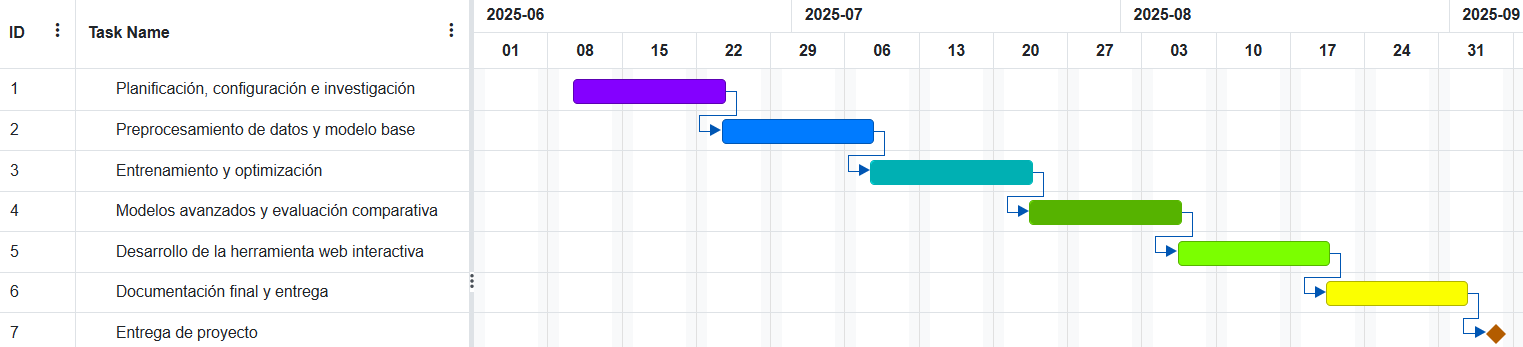
\includegraphics[width=1\textwidth]{figuras/diagrama_gantt/gantt.png}
  \caption{Diagrama de Gantt para la planificación del proyecto}
  \label{fig:diagrama_gantt}
\end{figure}


\chapter{Herramienta Web} %%%%%%%%%%%%%%%%%%%%%%%%%%%%%%%%%%%%%%%%%%%%%%%%%%%%%%%
\label{Herramienta Web anexo}

\section{Manual de usuario}
\label{Manual de usuario}

Para facilitar la interacción del usuario con la herramienta web vista con anterioridad, se define la siguiente guía de usuario.

Desde el entorno, con la dependencia \textit{Streamlit}, se ejecuta el comando \texttt{streamlit run app.py} y se lanza la aplicación en el navegador predeterminado
como se muestra en la siguiente imagen.

\begin{figure}[htbp]
  \centering
  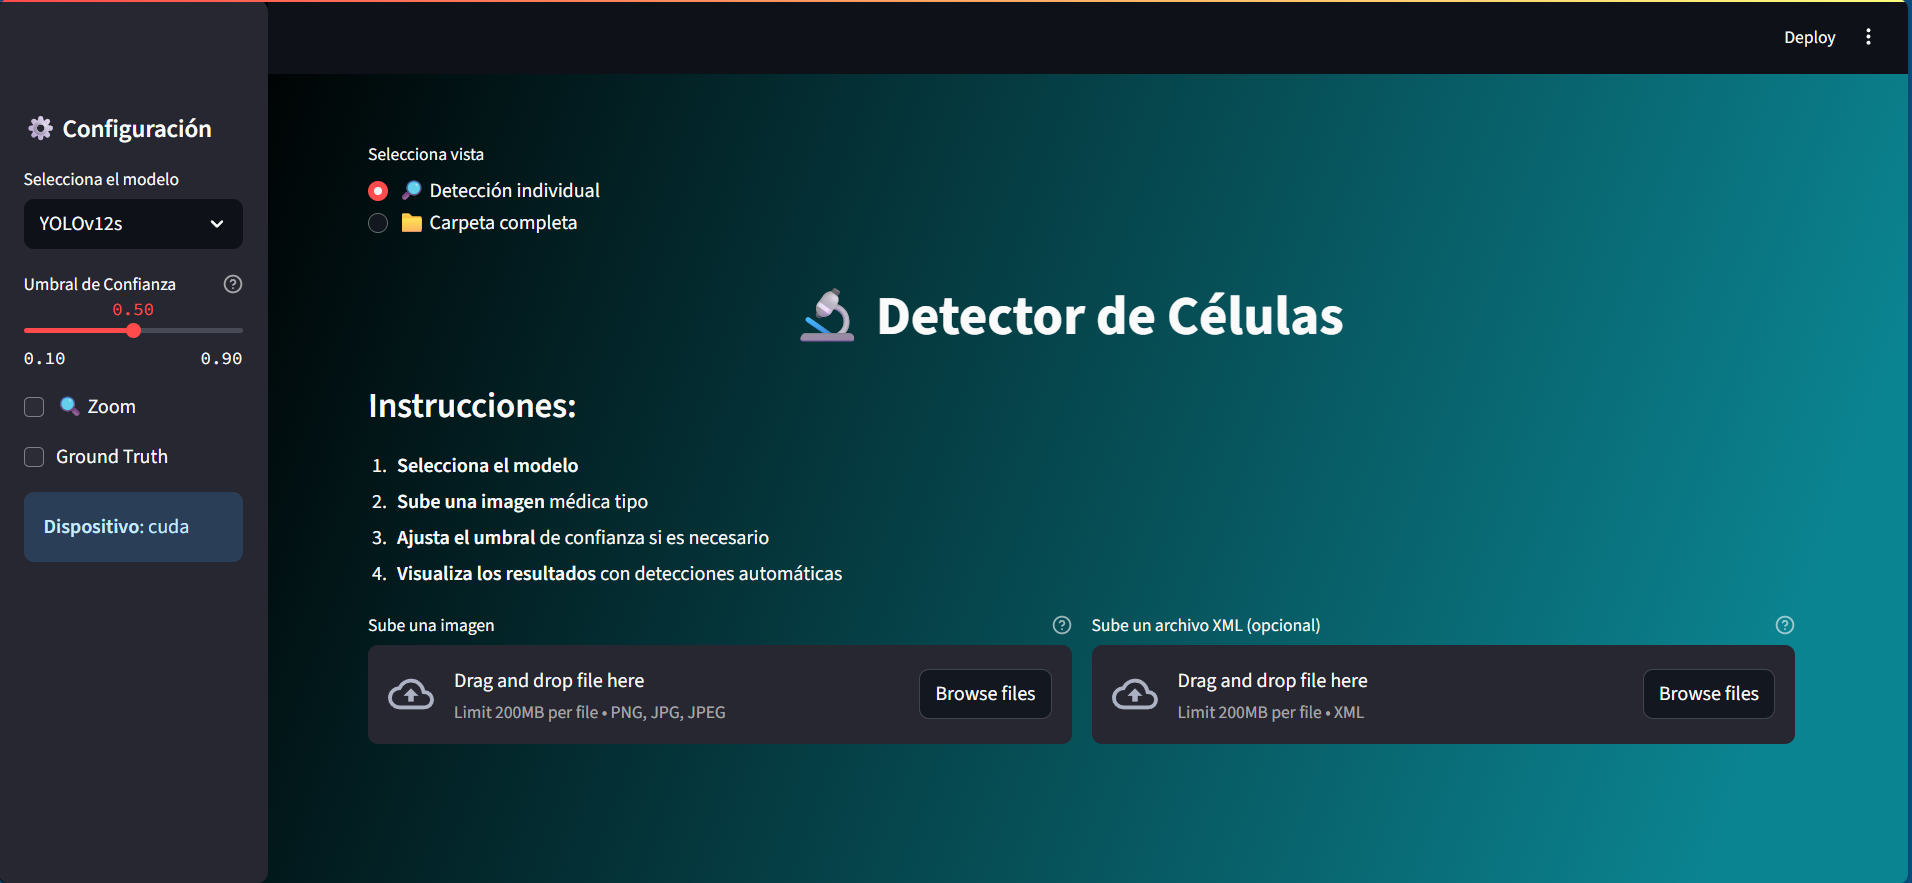
\includegraphics[width=1.0\textwidth]{figuras/app/cell_app.png}
  \caption{Interfaz de la aplicación web.}
  \label{fig:cell_app}
\end{figure}

En este punto, el usuario puede tomar la decisión de procesar una imagen individual o un conjunto de imágenes. Para esto, 
tenemos el \textit{widget} que permite la selección entre "Detección individual" o "Carpeta completa". En ambas situaciones,
la aplicación nos muestra una guia básica de funcionamiento en el apartado "Introducciones" en la \autoref{fig:cell_app}.
De manera totalmente opcional, el usuario puede cargar junto a la imagen a estudio, el correspondiente conjunto de anotaciones.

El \textit{widget} de "Configuración" permite la seleccion manual del modelo a través de un desplazable, el umbral de confianza de IoU, 
la representación del \textit{ground truth} (siempre que exista el xml asociado a la imagen) mediante un \textit{checkbox} (\autoref{fig:cell_app_gt}) y realizar un análisis exploratorio
sobre la imagen con un zoom (\autoref{fig:cell_app_zoom}). Asimismo, muestra el dispositivo (CPU o GPU) con el que se procesan las imágenes.

\begin{figure}[htbp]
  \centering
  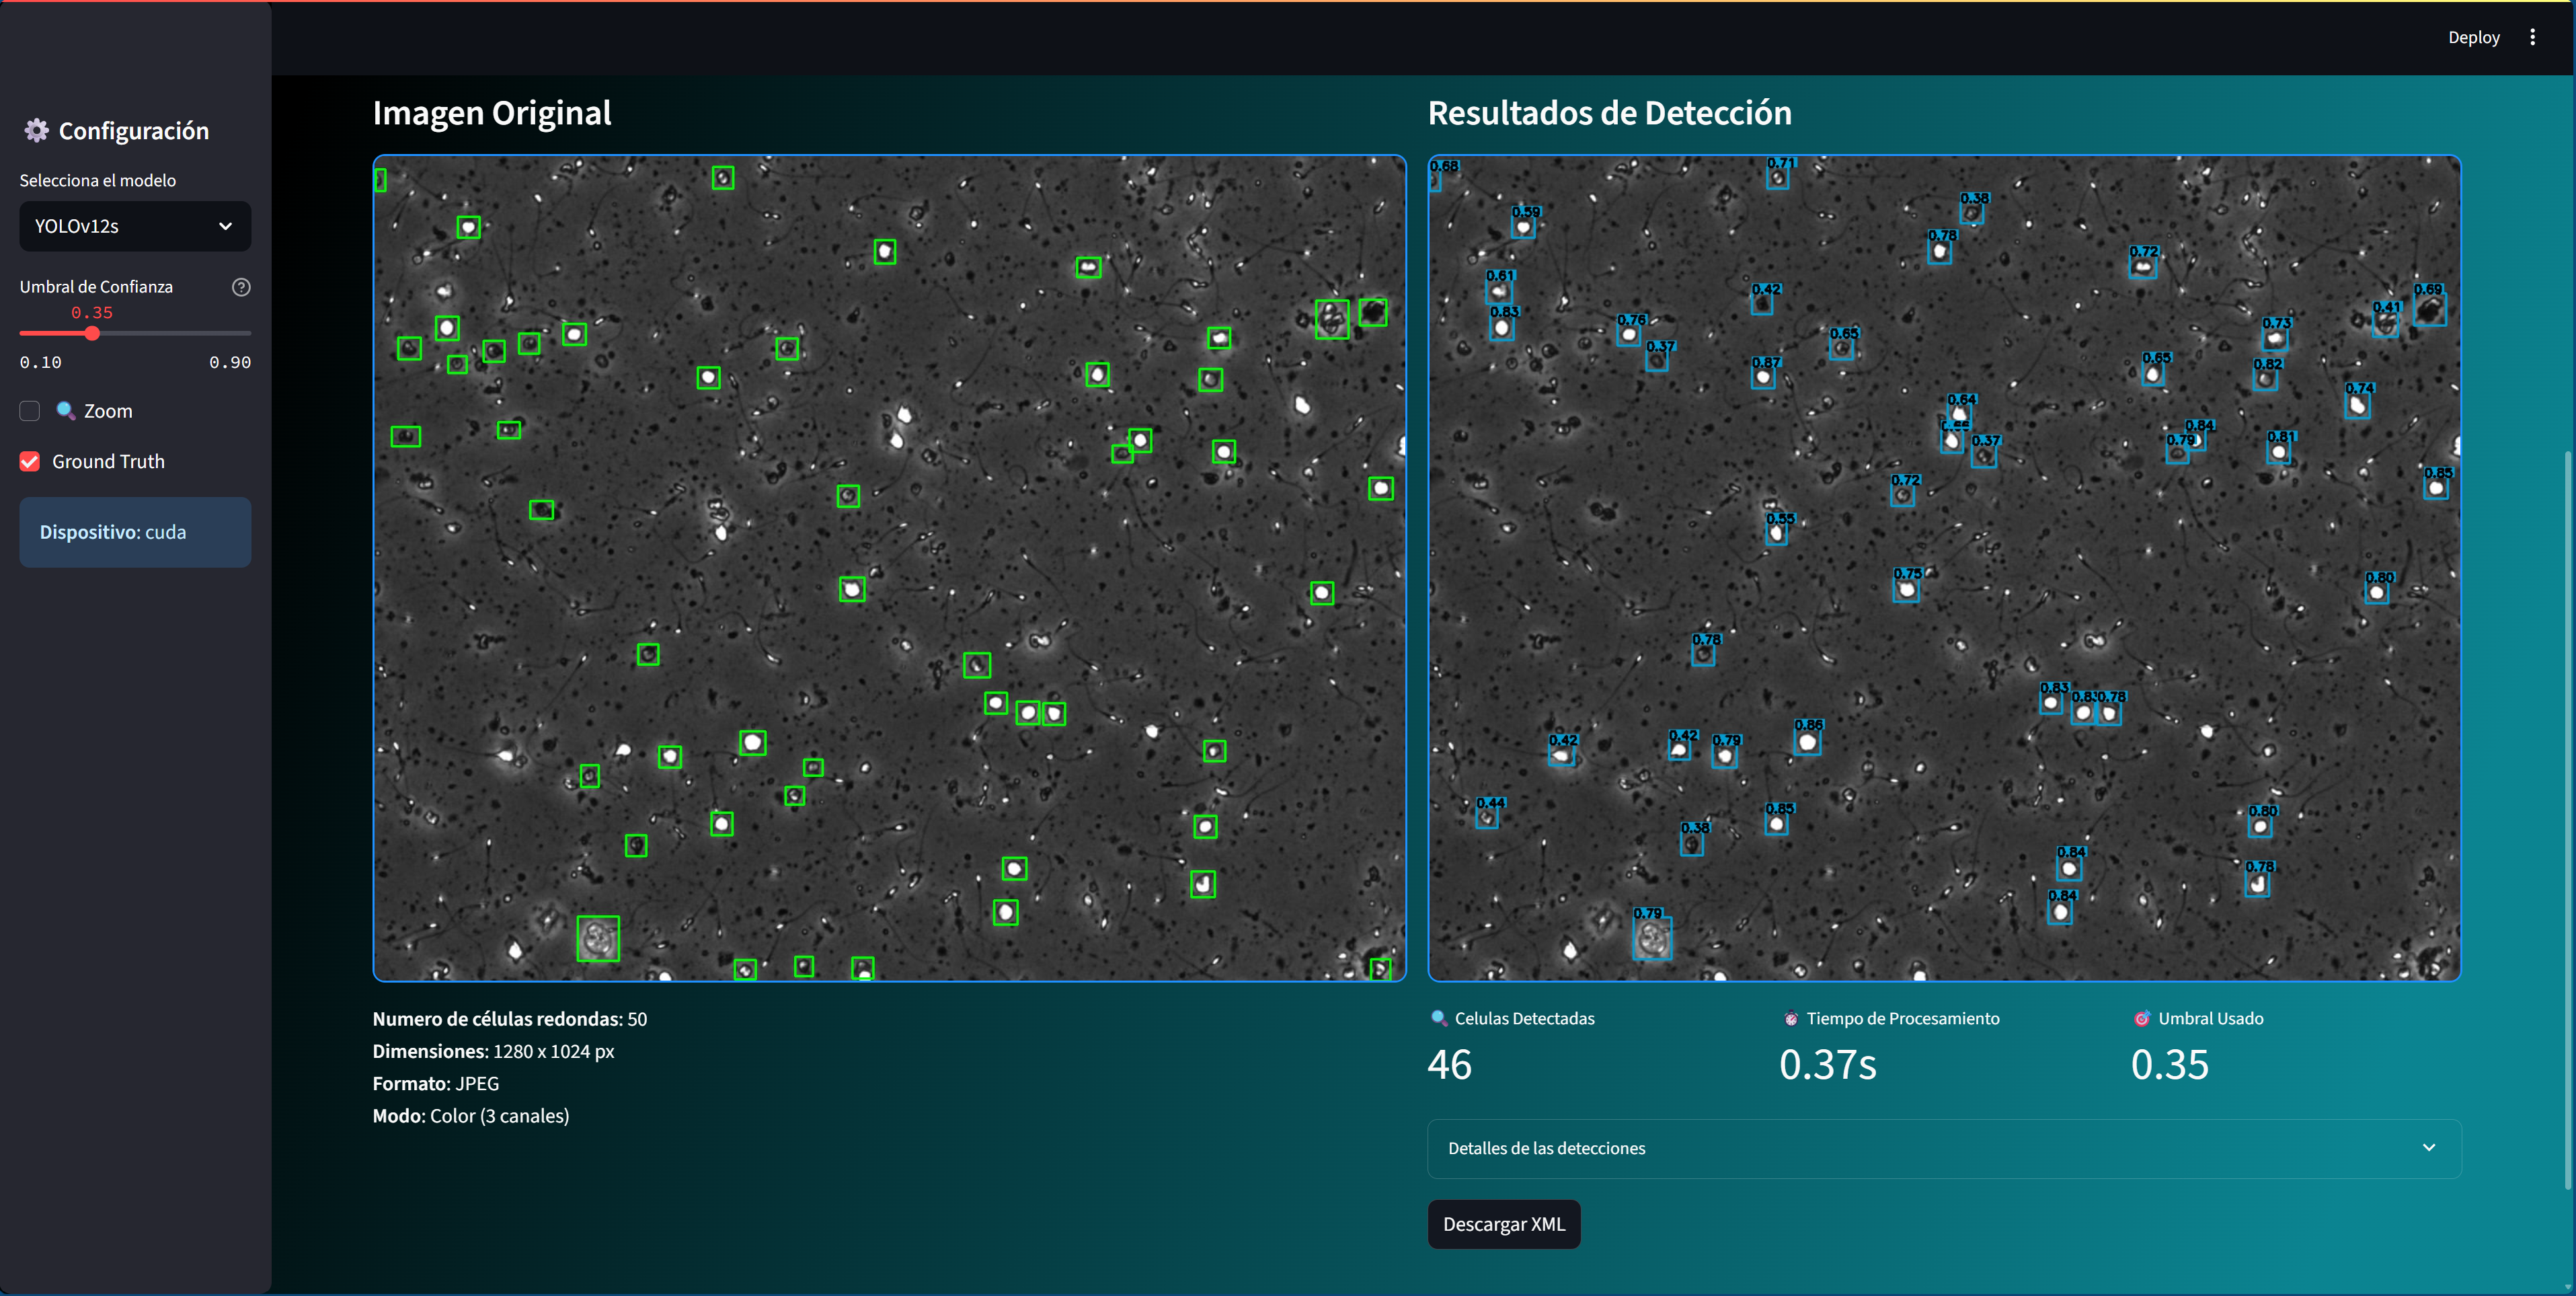
\includegraphics[width=1.0\textwidth]{figuras/app/prueba_imagen.png}
  \caption{Herramienta web: \textit{checkbox ground truth}.}
  \label{fig:cell_app_gt}
\end{figure}

\begin{figure}[htbp]
  \centering
  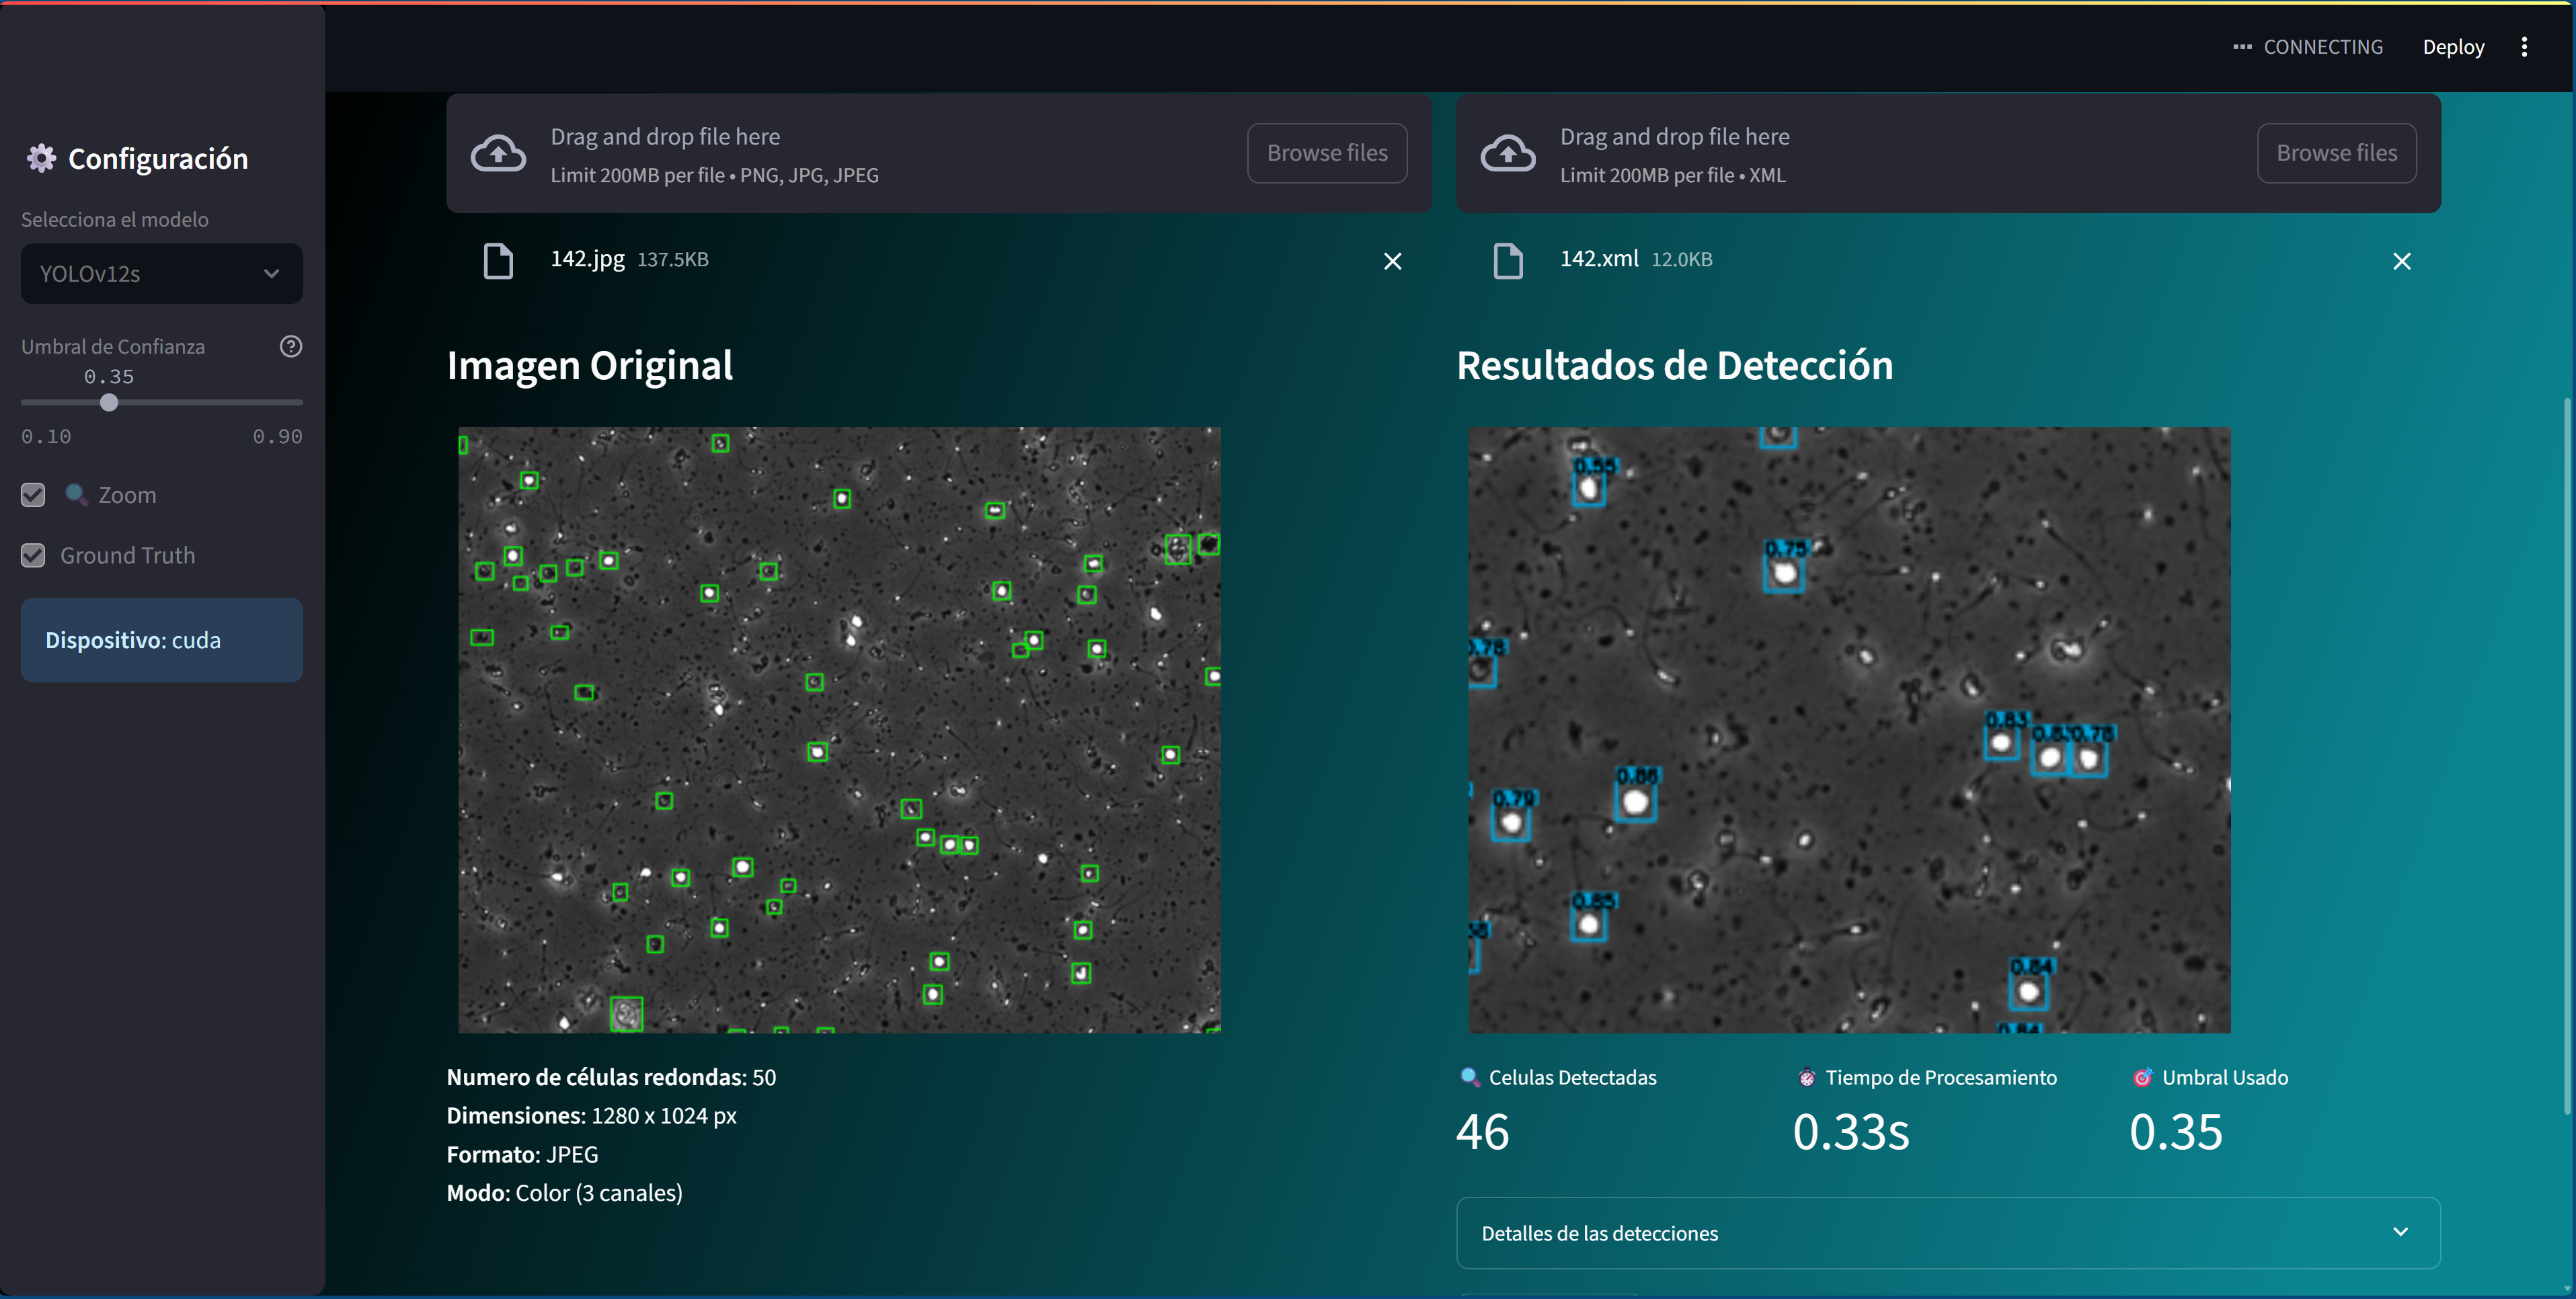
\includegraphics[width=1.0\textwidth]{figuras/app/zoom_imagen.png}
  \caption{Herramienta web: \textit{checkbox zoom}.}
  \label{fig:cell_app_zoom}
\end{figure}

Cabe destacar que el \textit{widget} "Descargar XML" permite al usuario descargar las predicciones del modelo realizadas sobre la imagen de entrada en un formato
PASCAL VOC. 

Si el usuario prefiere evaluar un conjunto de imágenes con sus respectivas anotaciones, se debe seleccionar la elección de "carpeta completa" como se muestra en la \autoref{fig:cell_app_directory}.

\begin{figure}[htbp]
  \centering
  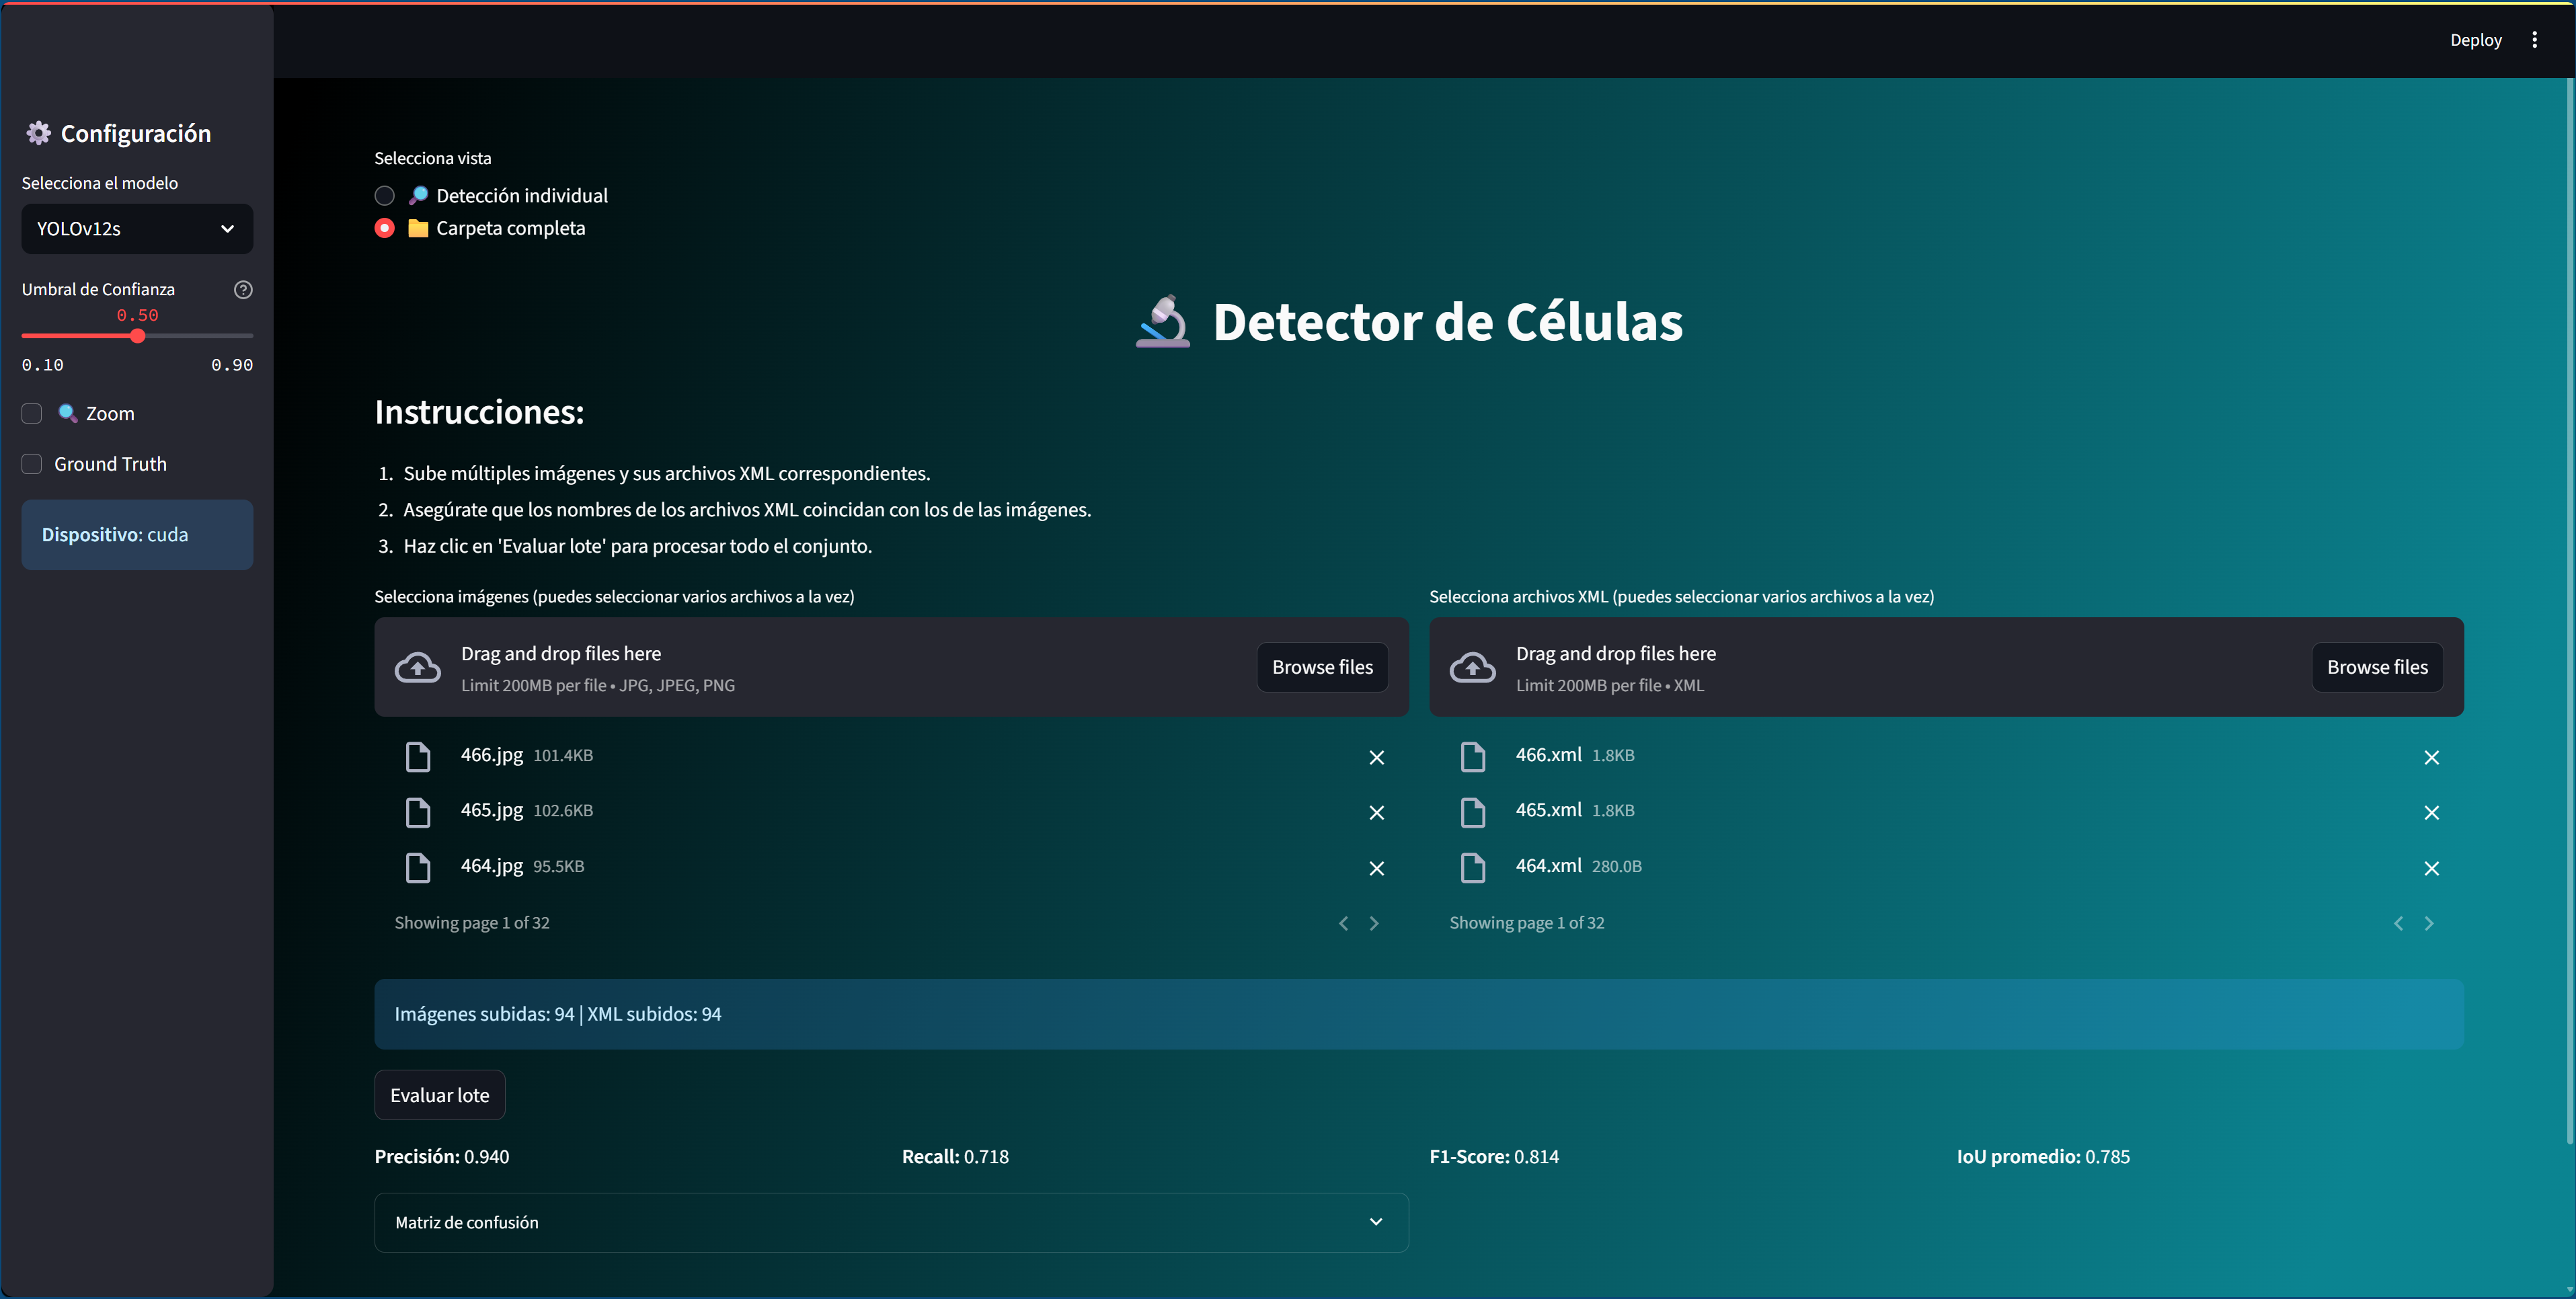
\includegraphics[width=1.0\textwidth]{figuras/app/cell_app_directorio.png}
  \caption{Herramienta web para procesar un conjunto de imágenes.}
  \label{fig:cell_app_directory}
\end{figure}

En este modo de evaluación, no está permitido el uso de los \textit{widgets}: \textit{ground truth} y \textit{zoom}. Sin embargo, 
el procesamiento del modelo seleccionado junto con su correspondiente umbral de confianza para el IoU, está acompañado de un pequeño conjunto de métricas:
\textit{precision}, \textit{recall}, \textit{F1-score} y \textit{mAP}. Para una mejor evaluación, la herramienta muestra una matriz de confusión (\autoref{fig:cell_app_metrics}).

\begin{figure}[htbp]
  \centering
  \includegraphics[width=1.0\textwidth]{figuras/app/matriz_confusión.png}
  \caption{Herramienta web: métricas y matriz de confusión.}
  \label{fig:cell_app_metrics}
\end{figure}

\section{Recomendaciones de uso}
\label{sec:Recomendaciones de uso}

A continuación, se recogen las pautas prácticas para el correcto funcionamiento de la herramienta web.

\begin{itemize}
  \item \textbf{Entorno recomendado:} se recomienda usar un entorno conda para tener aisladas las dependencias del proyecto y evitar así, conflictos entre dependencias. 
  Desde el directorio \texttt{04.Code} se proponen dos alternativas:
    \begin{itemize}
      \item Instalación del entorno completo con conda (recomendado):
        \begin{itemize}
          \item \texttt{conda env create -f environment.yml}
          \item \texttt{conda activate tfm\_env}
        \end{itemize}
      \item Instalación de un subconjunto de dependencias con conda:
        \begin{itemize}
          \item \texttt{conda create -n tfm\_env python=3.11 -y}
          \item \texttt{conda activate tfm\_env}
          \item \texttt{pip install -r 04.Codigo/requirements.txt}
        \end{itemize}
    \end{itemize}
  \item \textbf{Ejecución de la aplicación:} en la carpeta \texttt{04.Codigo/cell\_detection\_App} ejecutar:
    \begin{itemize}
      \item \texttt{streamlit run app.py}
      \item Automáticamente se abre en el navegador por defecto la URL que \textit{Streamlit} indique (por defecto \texttt{http://localhost:8501}).
    \end{itemize}
  \item \textbf{Compatibilidad con modelos:} limitada a modelos de YOLO \cite{ultralytics_models}. 
\end{itemize}

\section{Resolución de problemas}
\label{sec:Resolución de problemas}

Problemas que pueden tener lugar durante la instalación:

\begin{itemize}
  \item \textbf{La app no arranca o \textit{Streamlit} muestra error:}
    \begin{itemize}
      \item Verificar dependencias: \texttt{pip install -r 04.Codigo/requirements.txt}
      \item Comprobar la salida en el terminal donde se ejecuta \texttt{streamlit run app.py} y revisar trazas de error.
      \item Borrar caché de \textit{Streamlit}: \texttt{streamlit cache clear}.
    \end{itemize}
  \item \textbf{Modelo no encontrado o error de carga de pesos:}
    \begin{itemize}
      \item Confirmar que el fichero de pesos existe en \texttt{models/} y que la ruta es correcta (\path{04.Codigo/cell_detection_App/models/}).
    \end{itemize}
  \item \textbf{Problemas con GPU o CUDA:}
    \begin{itemize}
      \item Comprobar estado de la GPU: ejecutar \texttt{nvidia-smi} en terminal.
      \item Verificar que PyTorch detecta la GPU: 
        \begin{itemize}
          \item \texttt{python -c "import torch; print(torch.cuda.is\_available())"}
        \end{itemize}
      \item Si falla, forzar ejecución en CPU desde la UI o variable de entorno: \texttt{CUDA\_VISIBLE\_DEVICES=""}.
    \end{itemize}
  \item \textbf{Errores al procesar imágenes o XML mal formados:}
    \begin{itemize}
      \item Validar que las imágenes están en formatos soportados (\texttt{.jpg, .jpeg, .png}) y que los XML cumplen con el formato PASCAL VOC.
      \item Revisar el log de parsing en \texttt{04.Codigo/cell\_detection\_App/utils/} y corregir los ficheros señalados.
    \end{itemize}
\end{itemize}


\chapter{Evaluación comparativa de arquitecturas} %%%%%%%%%%%%%%%%%%%%%%%%%%%%%%%%%%%%%%%%%%%%%%%%%%%%%%%
\label{Evaluación comparativa de arquitecturas}

En este anexo, se recojen las representaciones gráficas para la evaluación de los modelos sobre los diferentes conjuntos de \textit{test}. Todas las representaciones en las que no se hace notar el IoU
de confianza del modelo, tienen por defecto un IoU de $0,5$. Las representaciones a evaluar recogen información a través de matrices de confusión, curva F1-confianza y resultados cualitativos del modelo en tiempo real.

\section{Matrices de confusión}
\label{sec:Matrice de confusión}

\begin{figure}[H]
  \centering
  \vspace{-0.3cm}
  % Primera fila
  \begin{subfigure}[b]{0.45\textwidth}
    \centering
    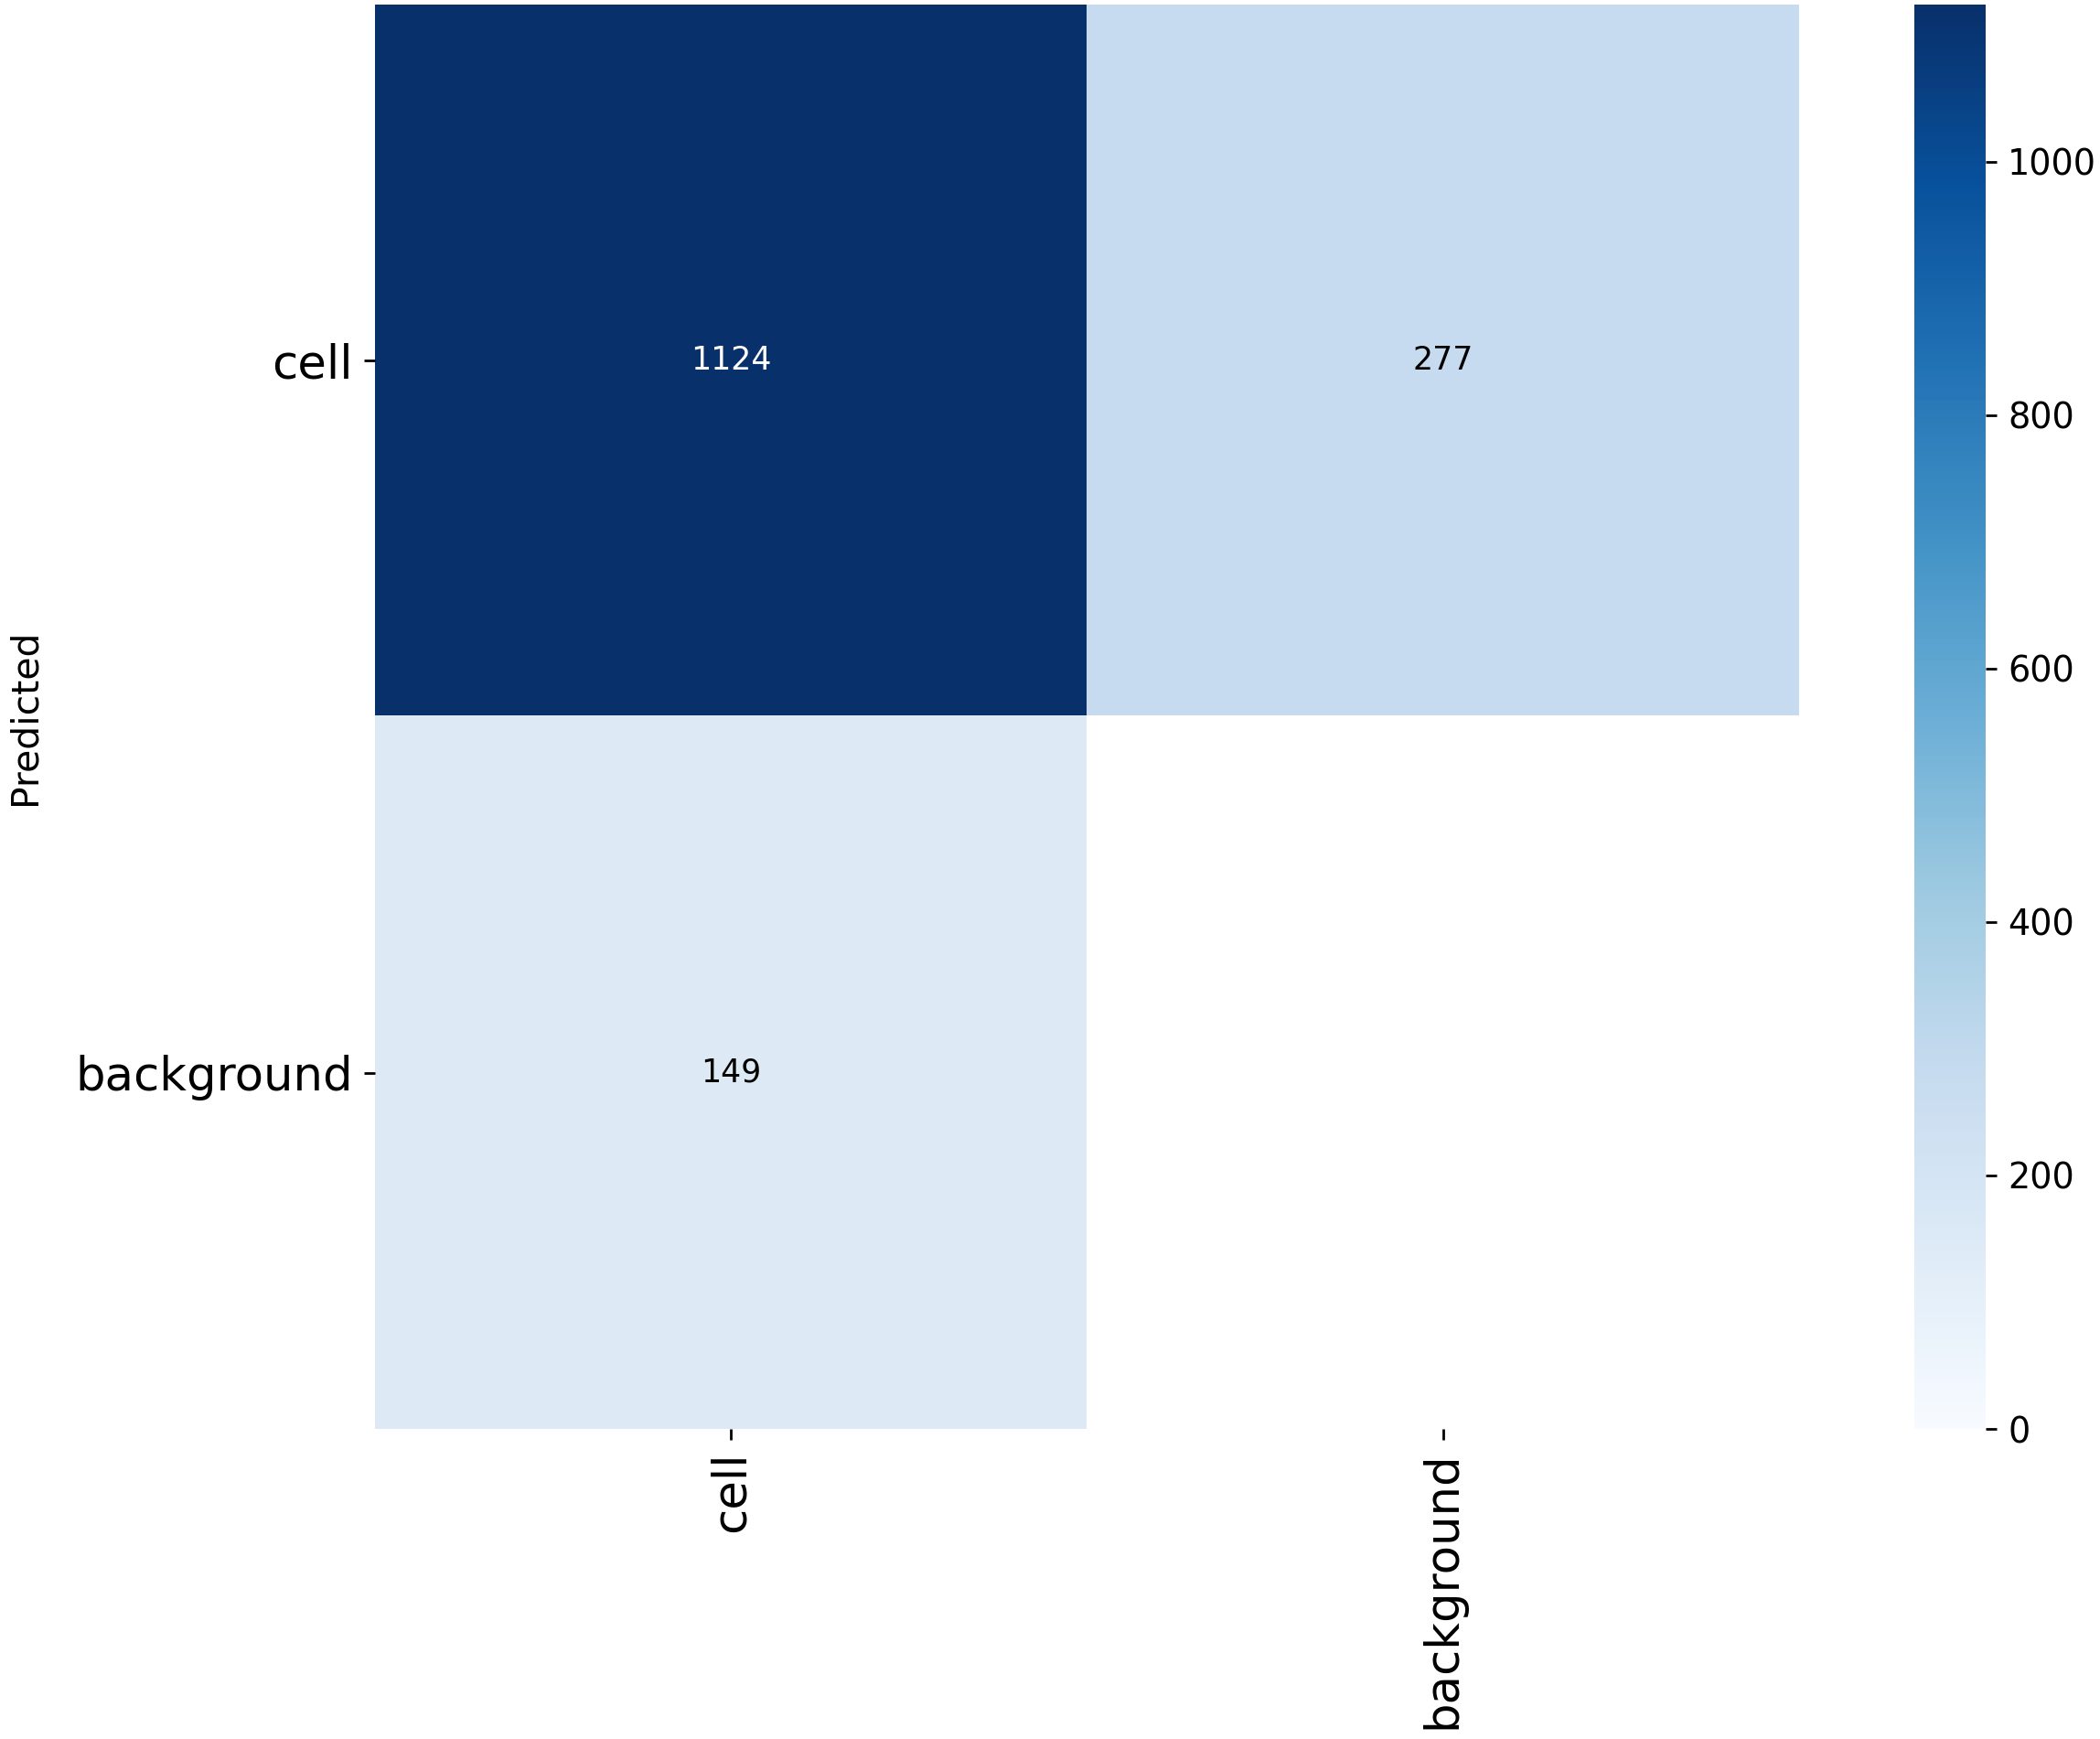
\includegraphics[height=5cm]{figuras/resultados experimentacion/yolov8s/original_test/confusion_matrix.png}
    \vspace{-0.3cm}
    \caption{\footnotesize YOLOv8s}
    \label{fig:confusion_yolov8s_original_test}
  \end{subfigure}
  \hfill
  \begin{subfigure}[b]{0.45\textwidth}
    \centering
    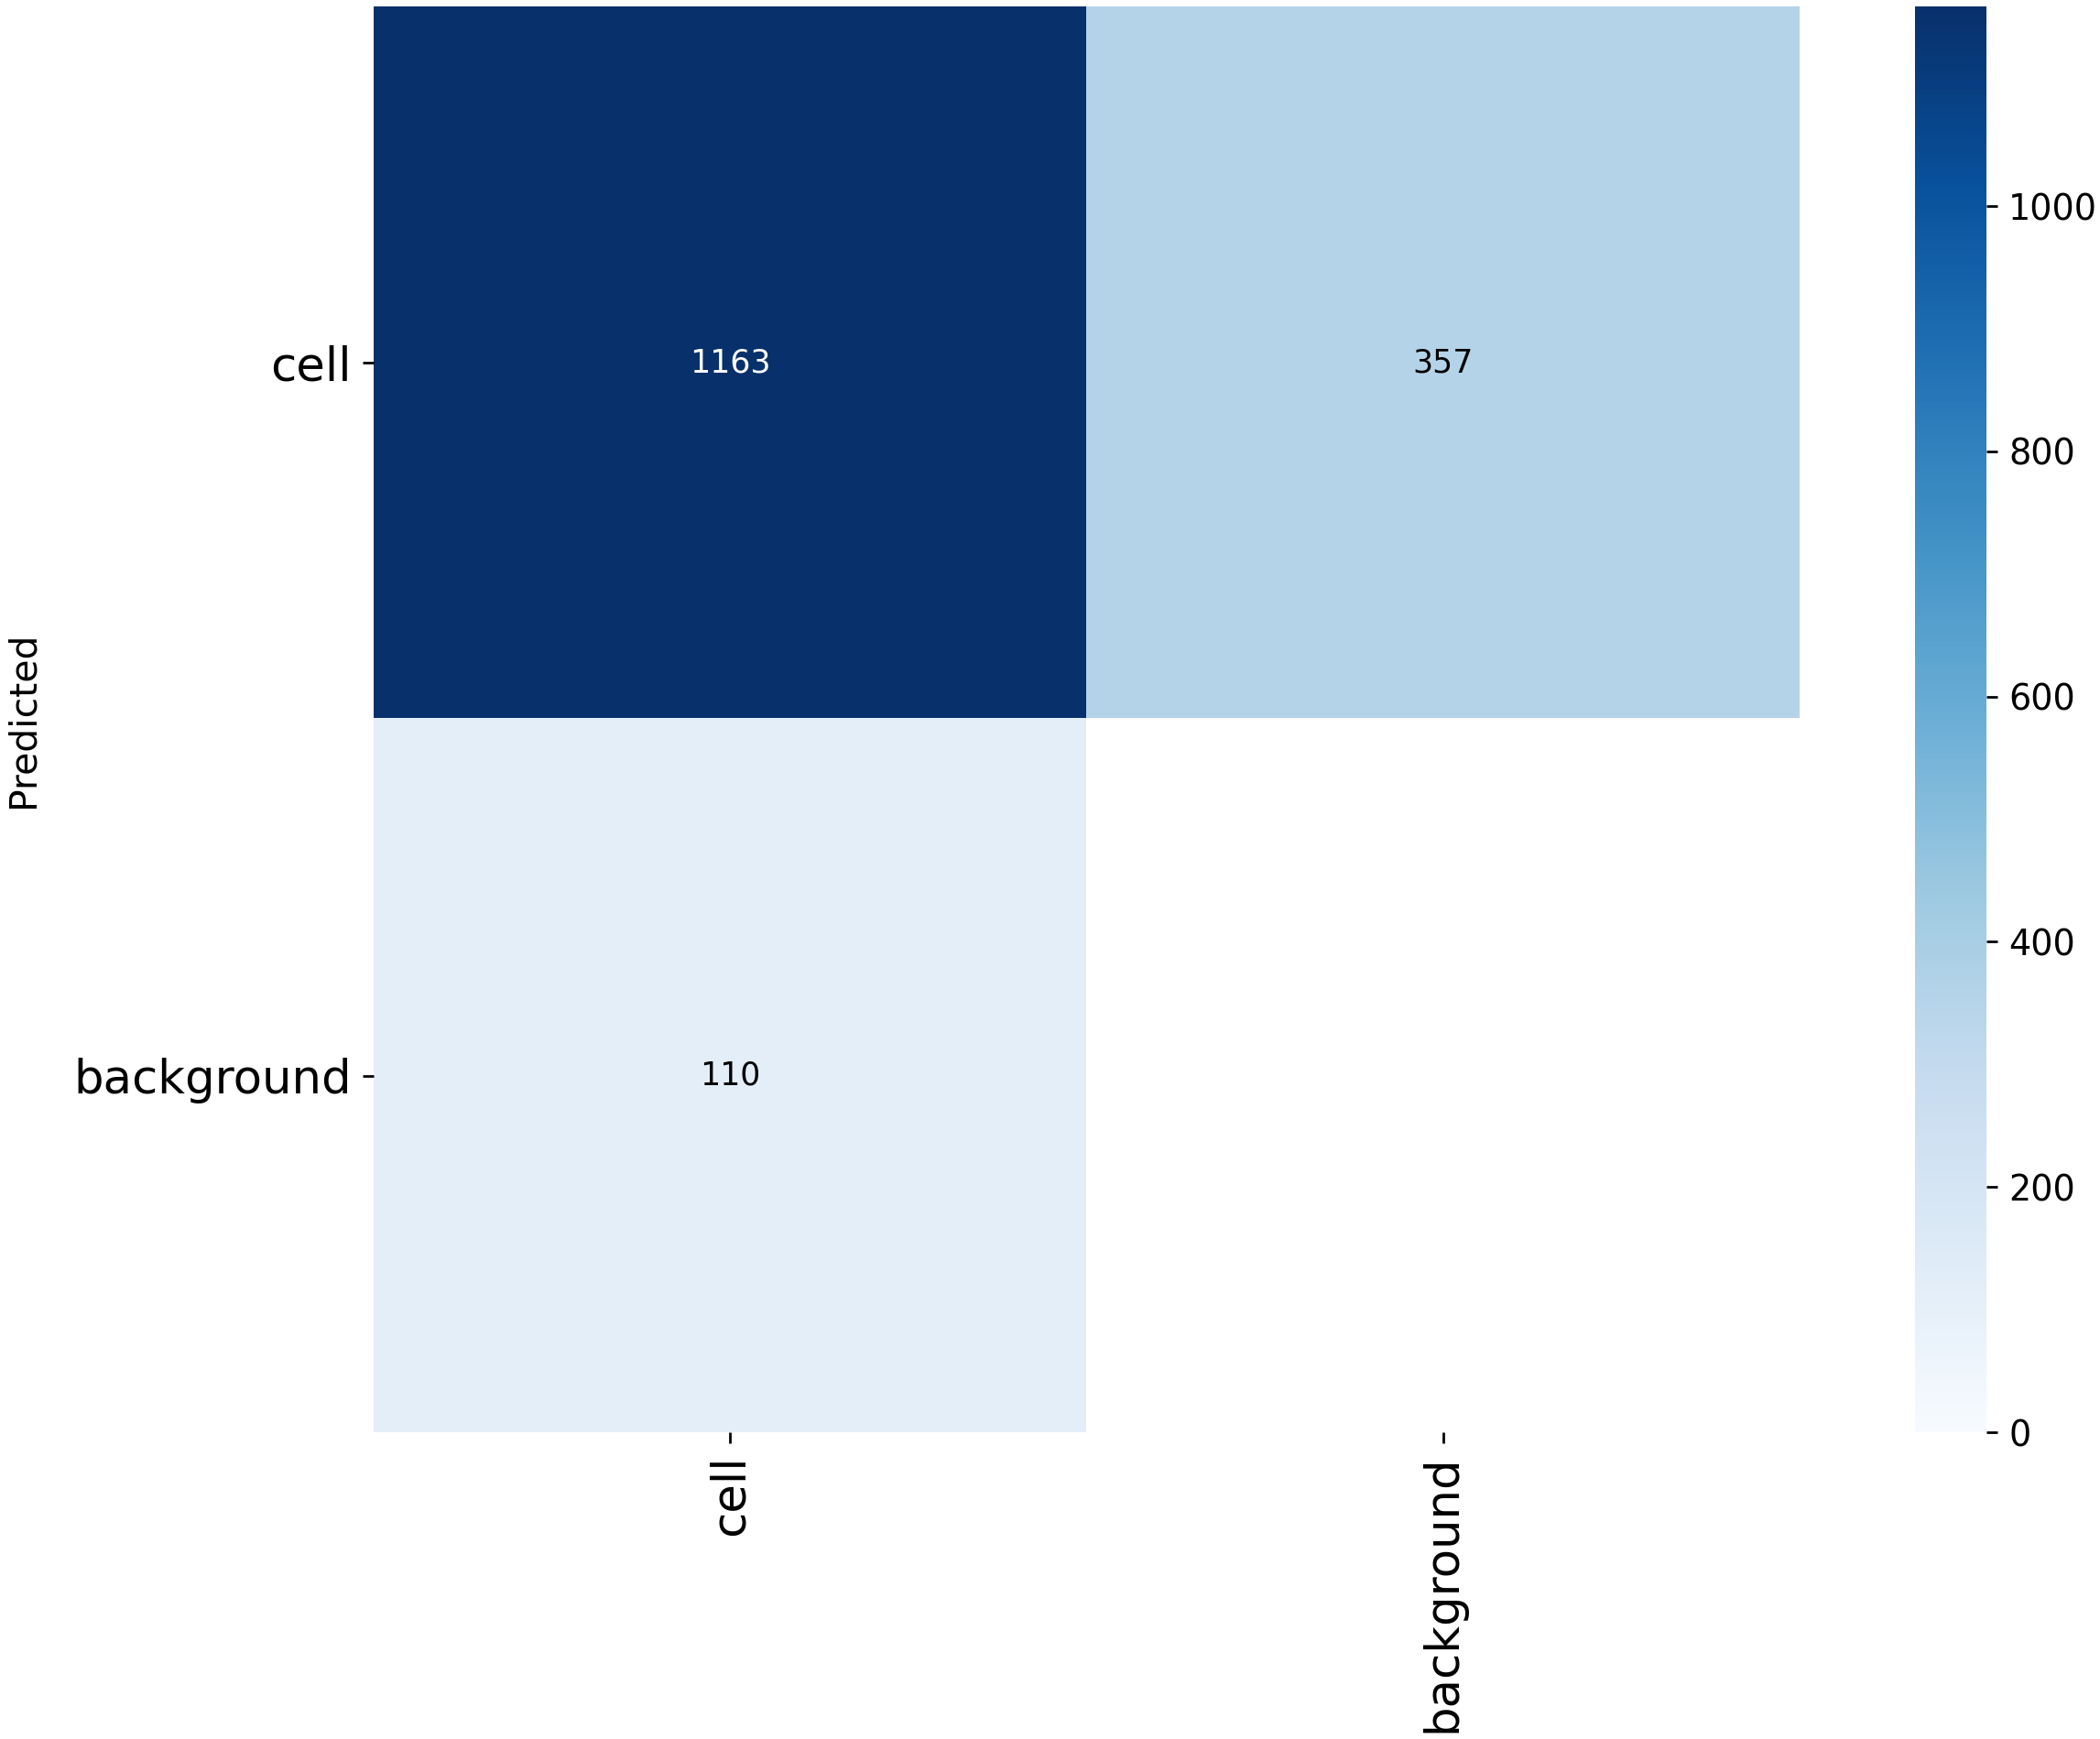
\includegraphics[height=5cm]{figuras/resultados experimentacion/yolov9s/original_test/confusion_matrix.png}
    \vspace{-0.3cm}
    \caption{\footnotesize YOLOv9s}
    \label{fig:confusion_yolov9s_original_test}
  \end{subfigure}
  
  \vspace{0.1cm}
  % Segunda fila
  \begin{subfigure}[b]{0.45\textwidth}
    \centering
    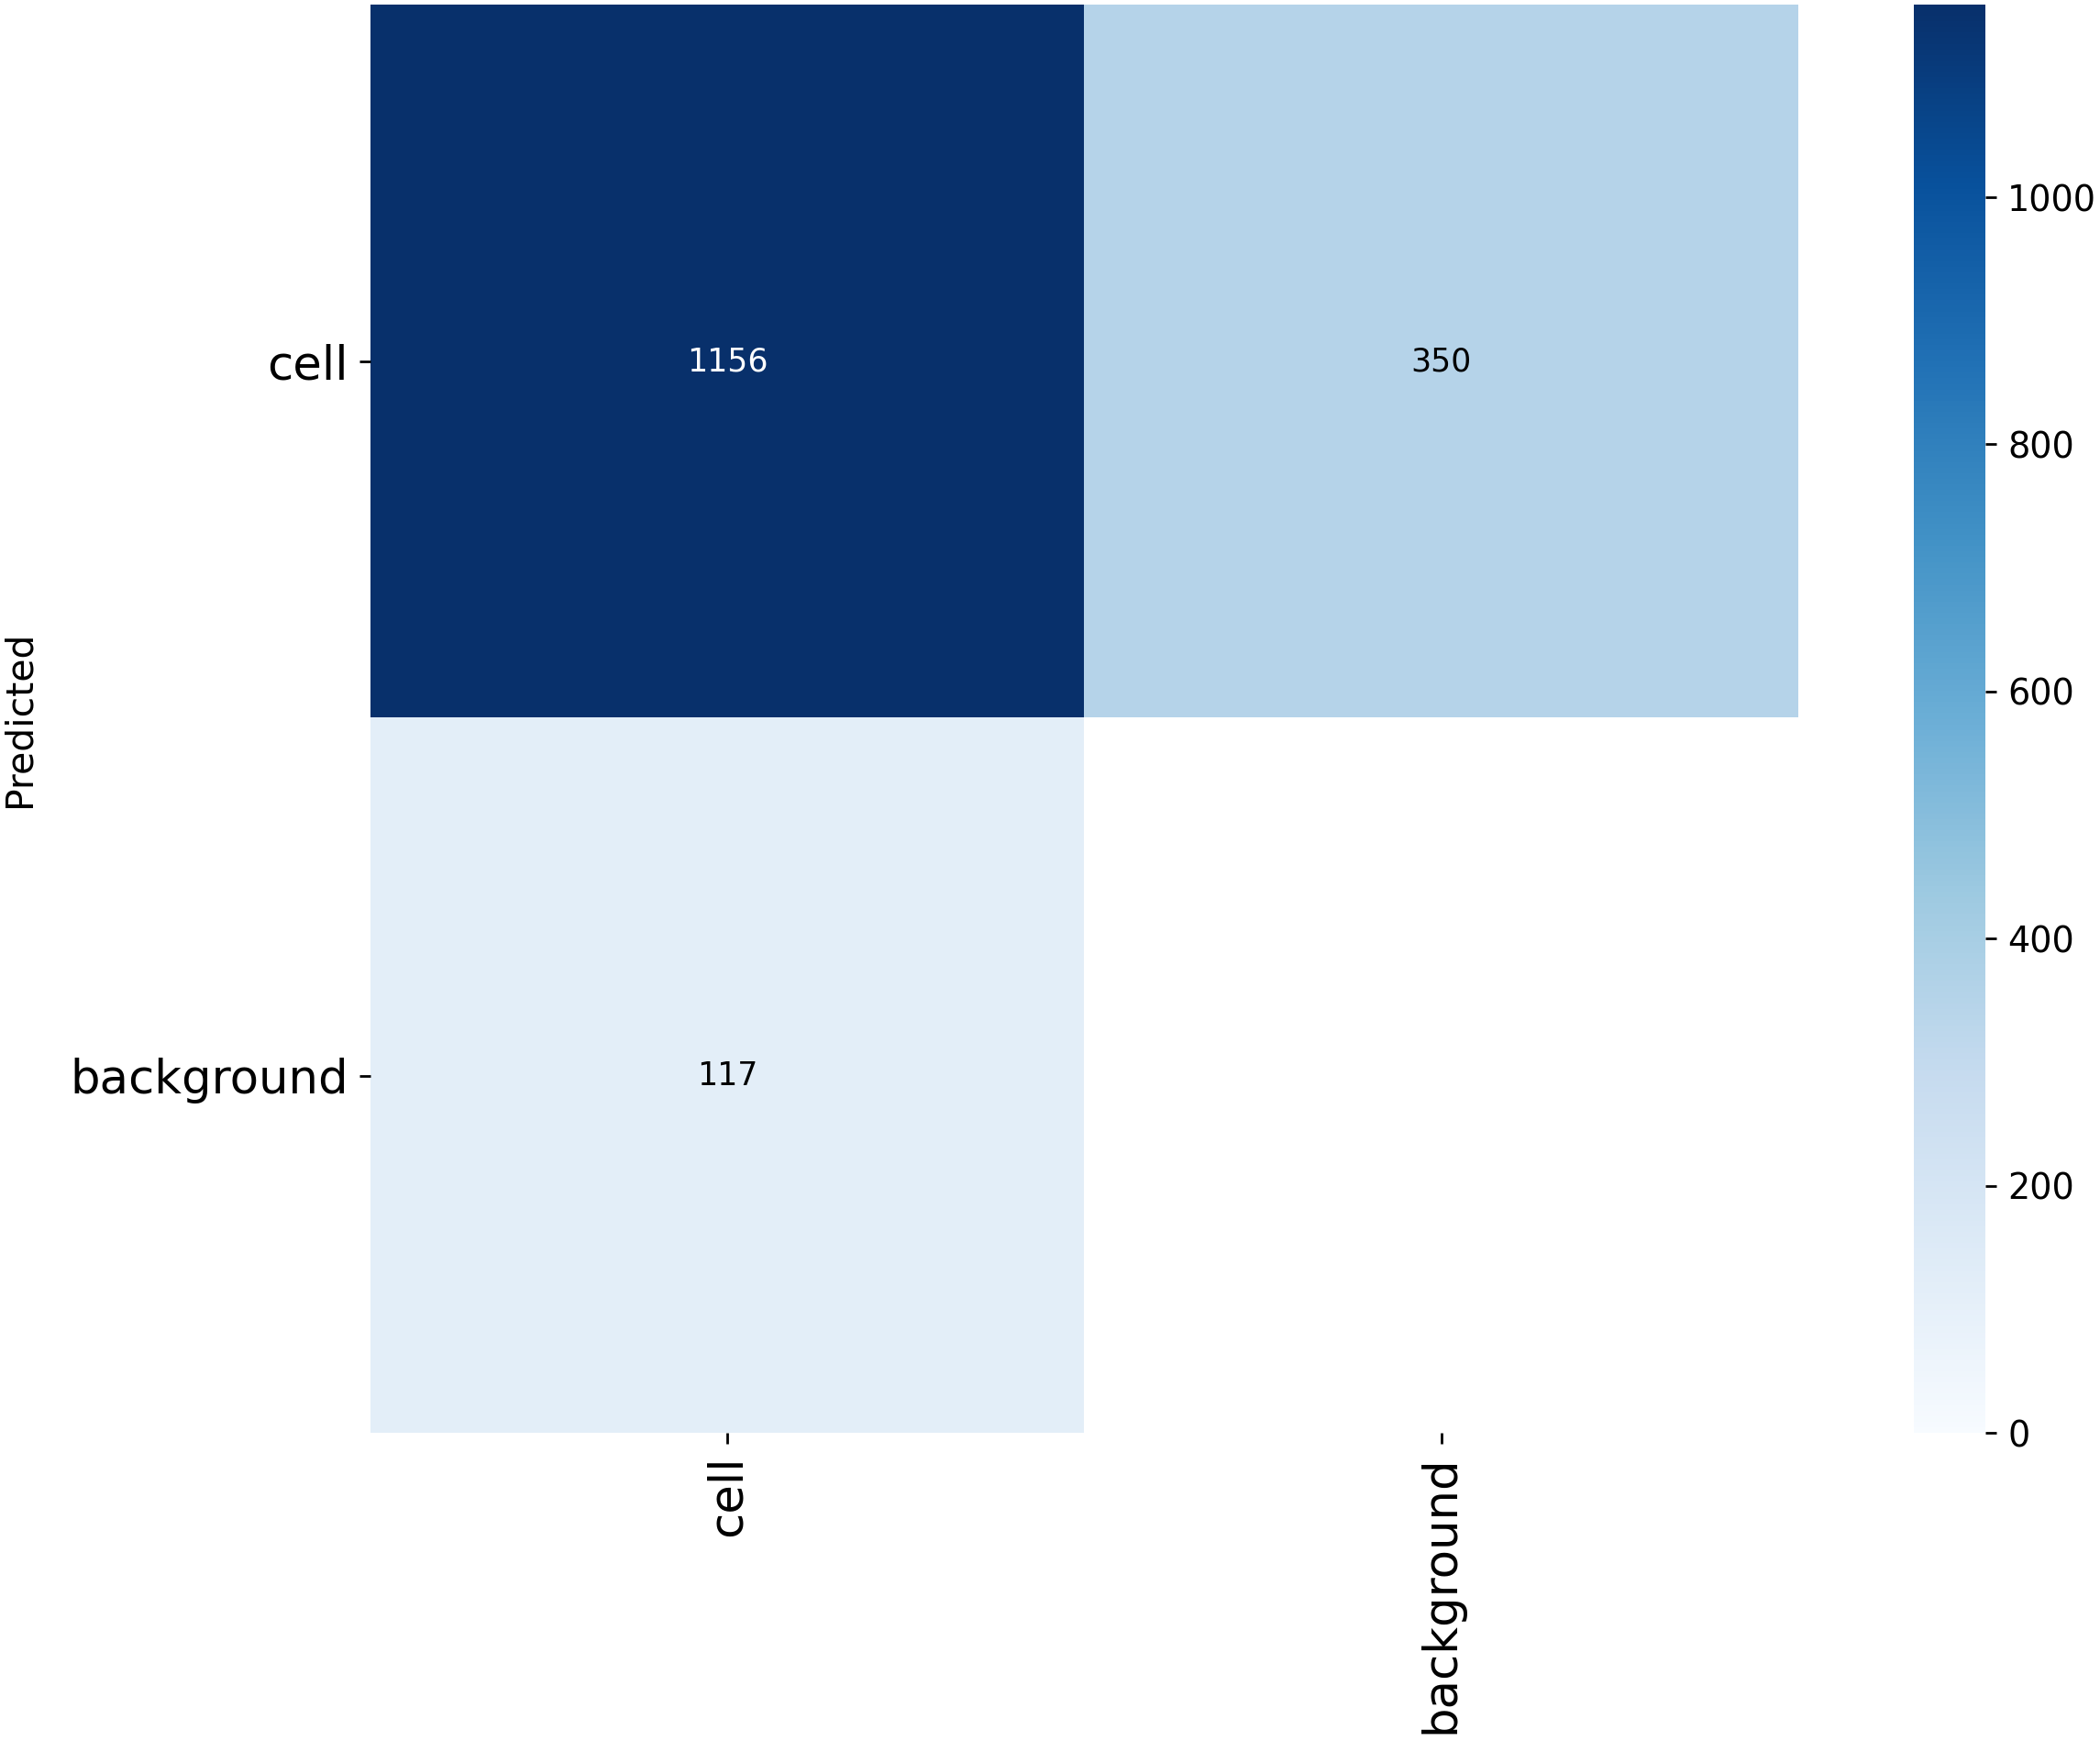
\includegraphics[height=5cm]{figuras/resultados experimentacion/yolov10s/original_test/confusion_matrix.png}
    \vspace{-0.3cm}
    \caption{\footnotesize YOLOv10s}
    \label{fig:confusion_yolov10s_original_test}
  \end{subfigure}
  \hfill
  \begin{subfigure}[b]{0.45\textwidth}
    \centering
    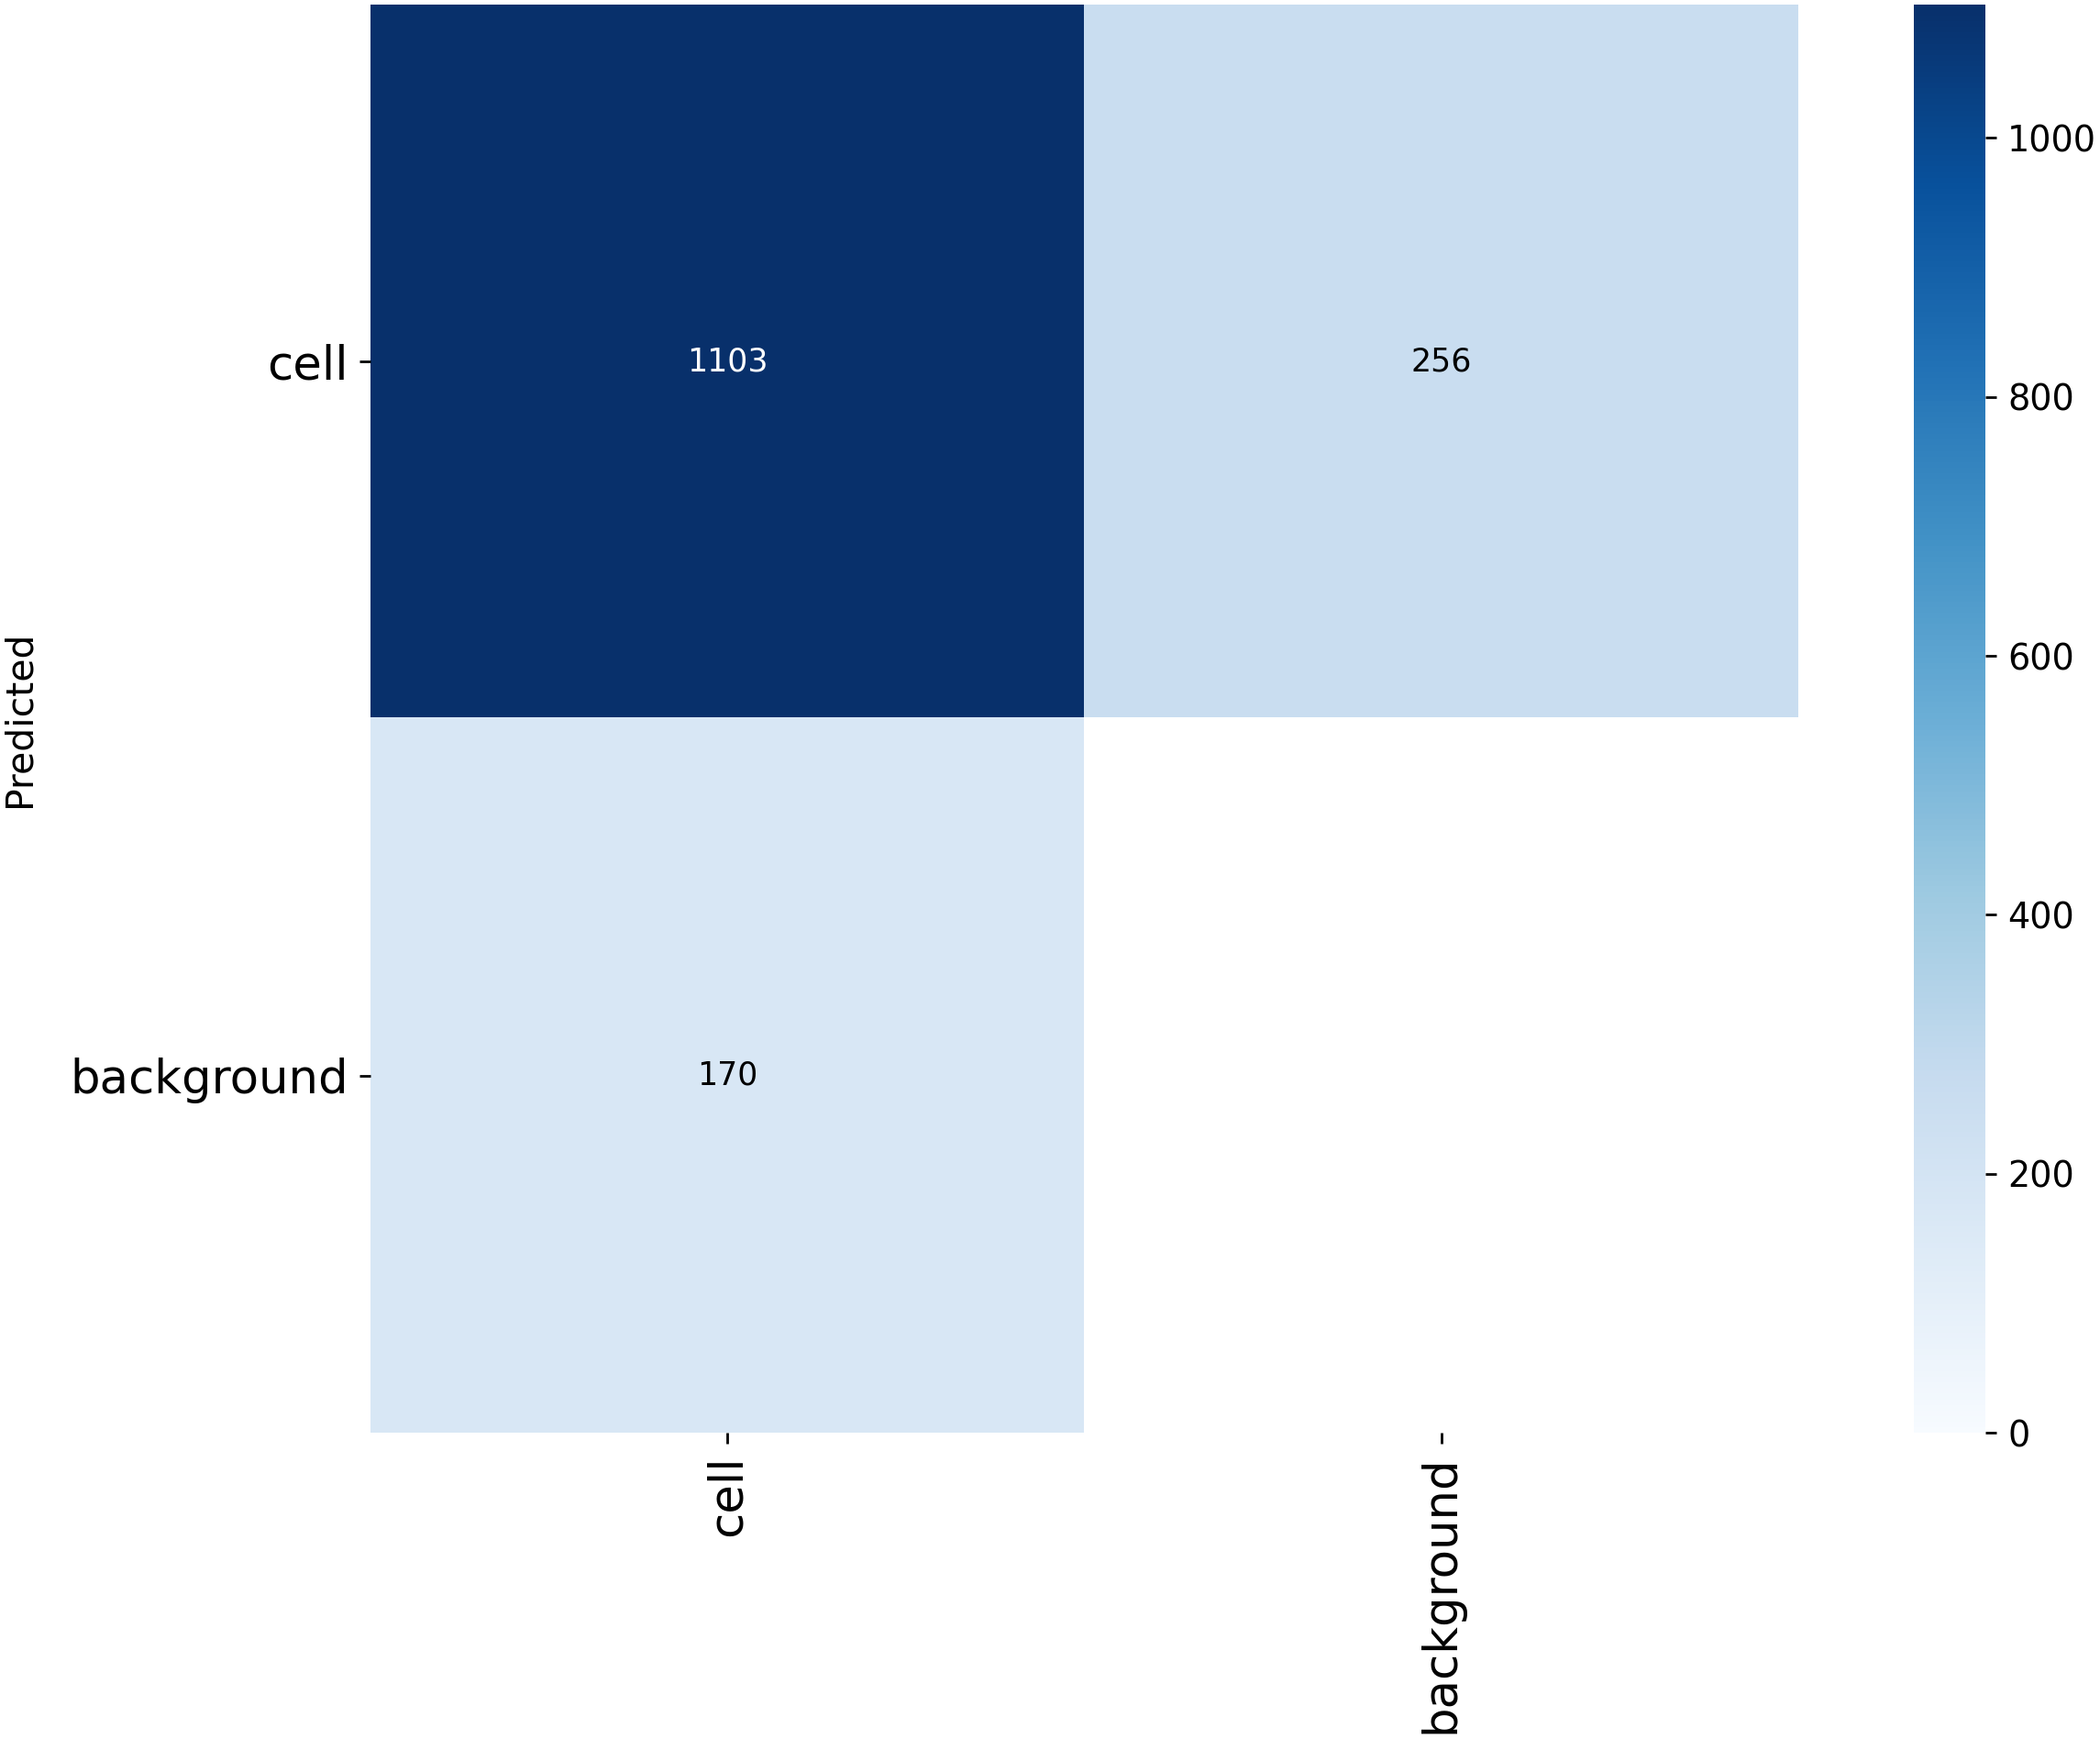
\includegraphics[height=5cm]{figuras/resultados experimentacion/yolov11s/original_test/confusion_matrix.png}
    \vspace{-0.3cm}
    \caption{\footnotesize YOLOv11s}
    \label{fig:confusion_yolov11s_original_test}
  \end{subfigure}
  
  \vspace{0.1cm}
  % Tercera fila
  \begin{subfigure}[b]{0.45\textwidth}
    \centering
    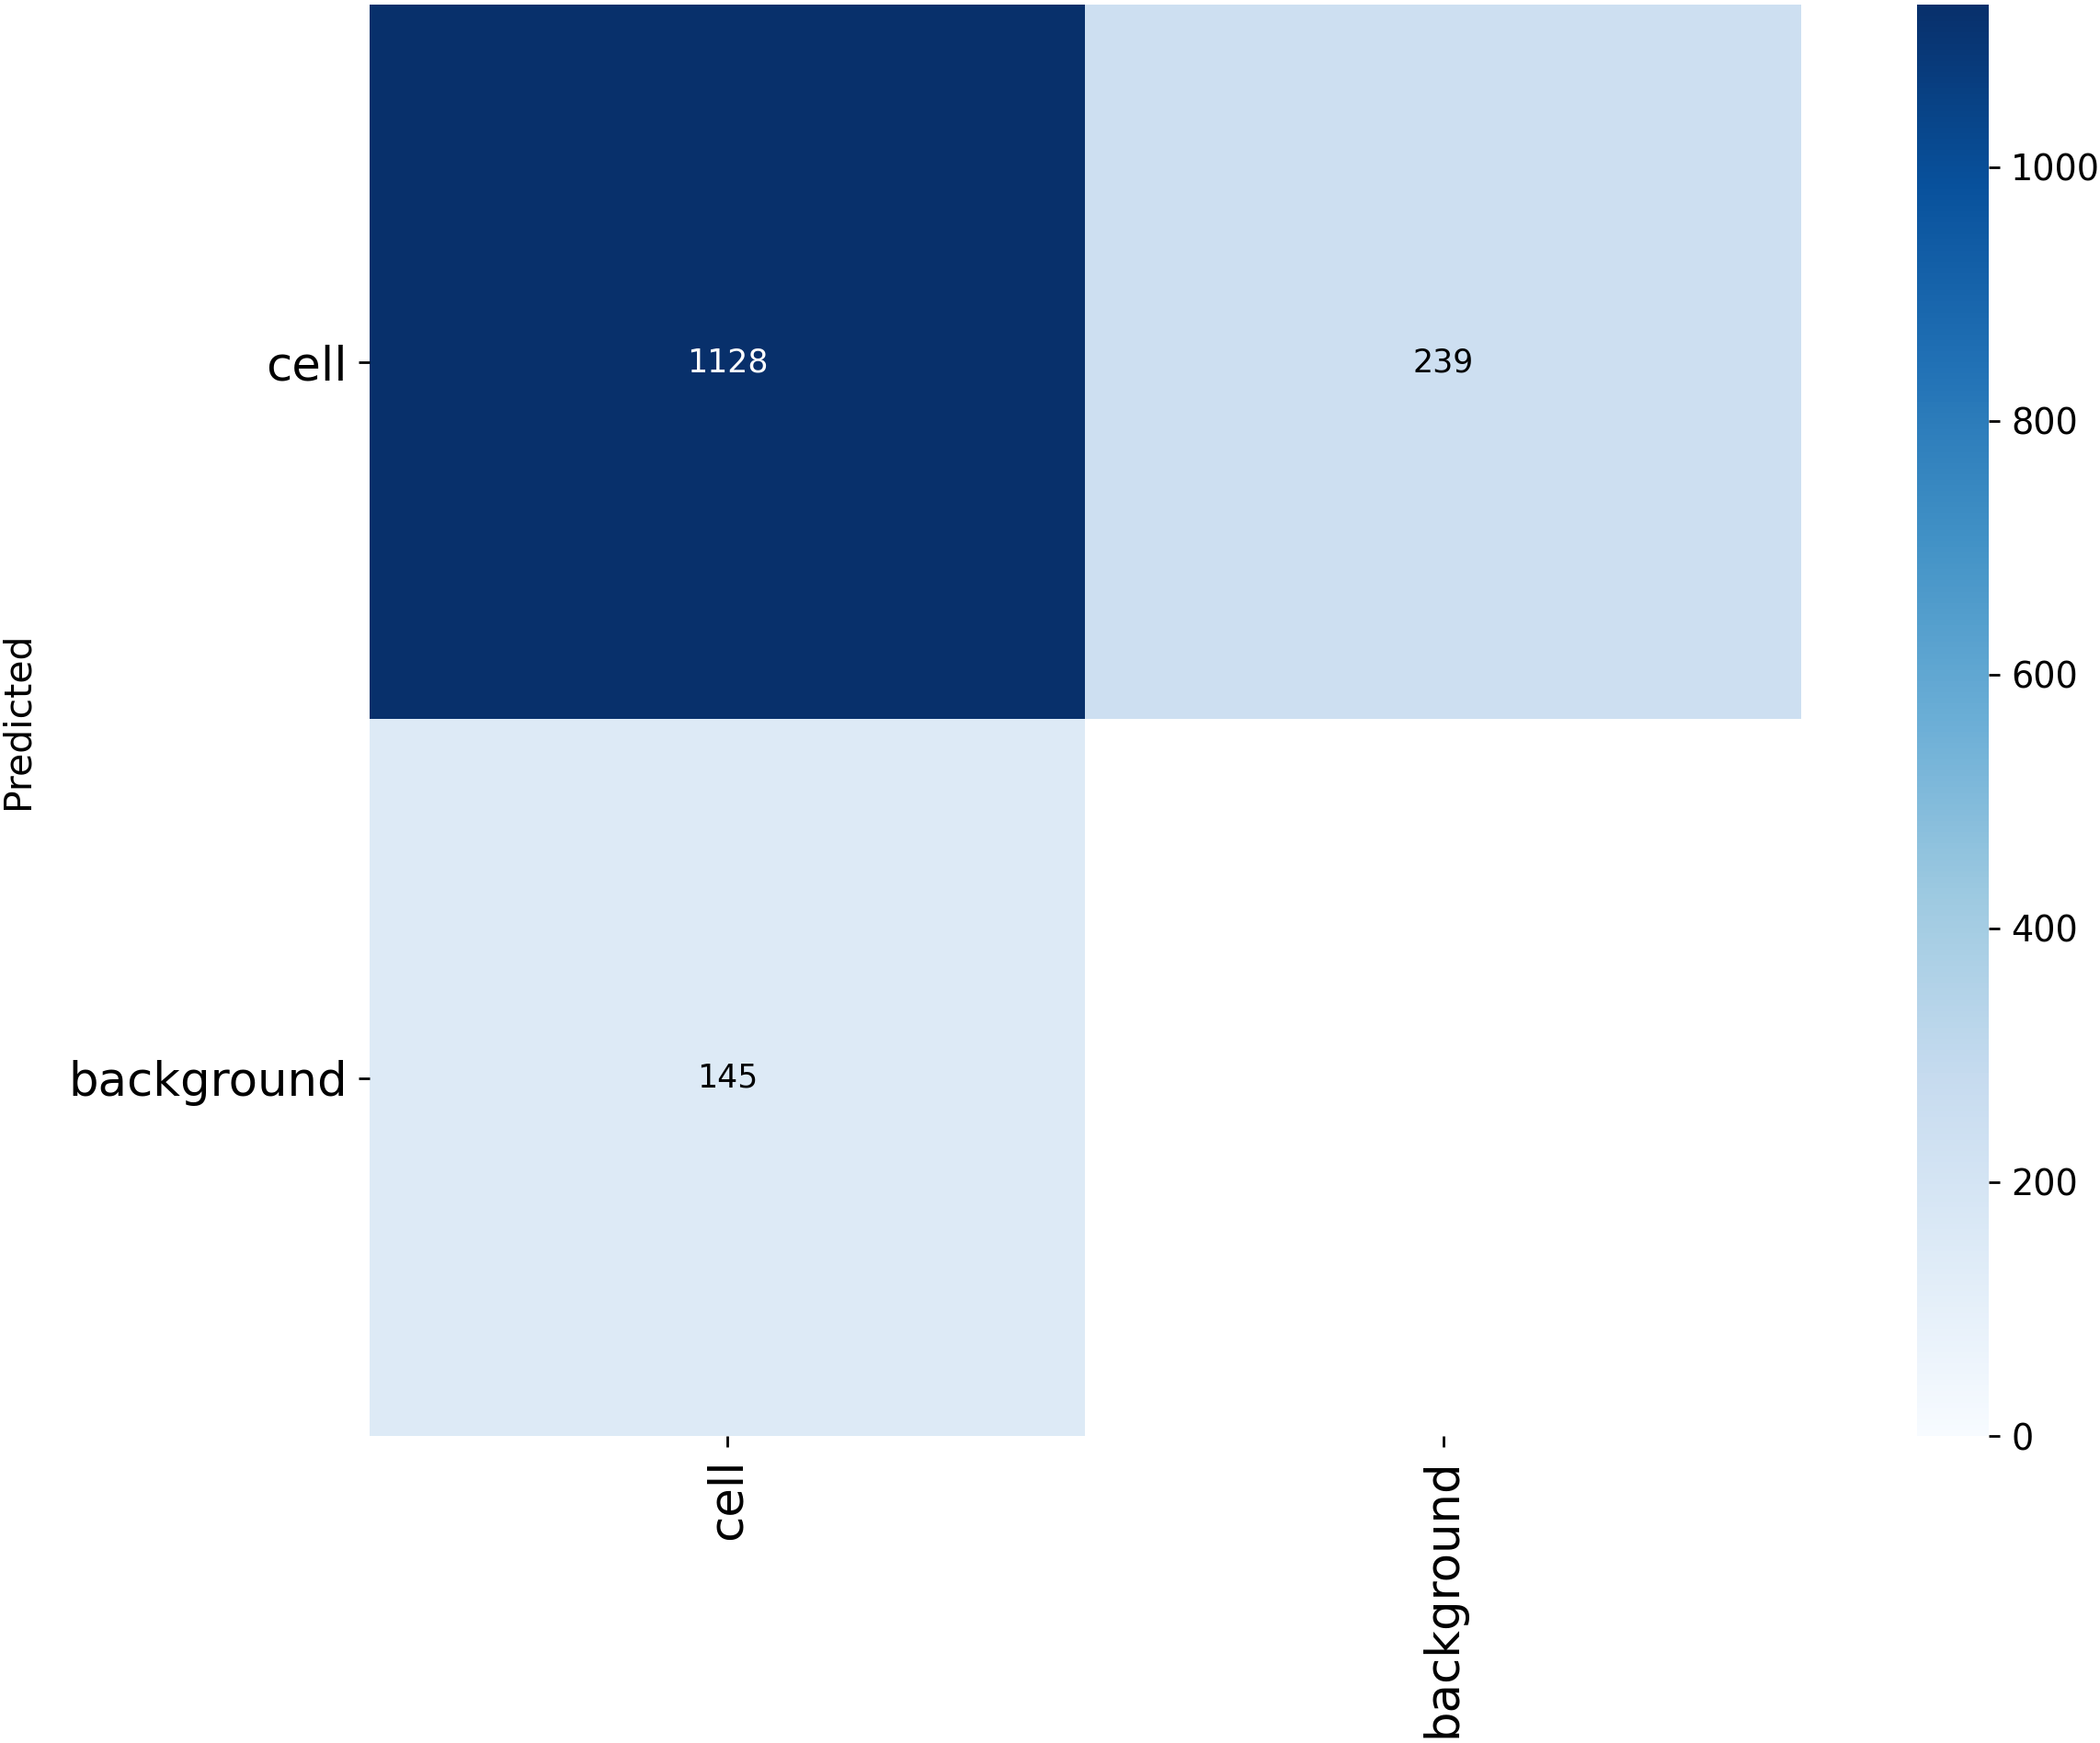
\includegraphics[height=5cm]{figuras/resultados experimentacion/yolov12s/original_test/confusion_matrix.png}
    \vspace{-0.3cm}
    \caption{\footnotesize YOLOv12s}
    \label{fig:confusion_yolov12s_original_test}
  \end{subfigure}
  \hfill
  \begin{subfigure}[b]{0.45\textwidth}
    \centering
    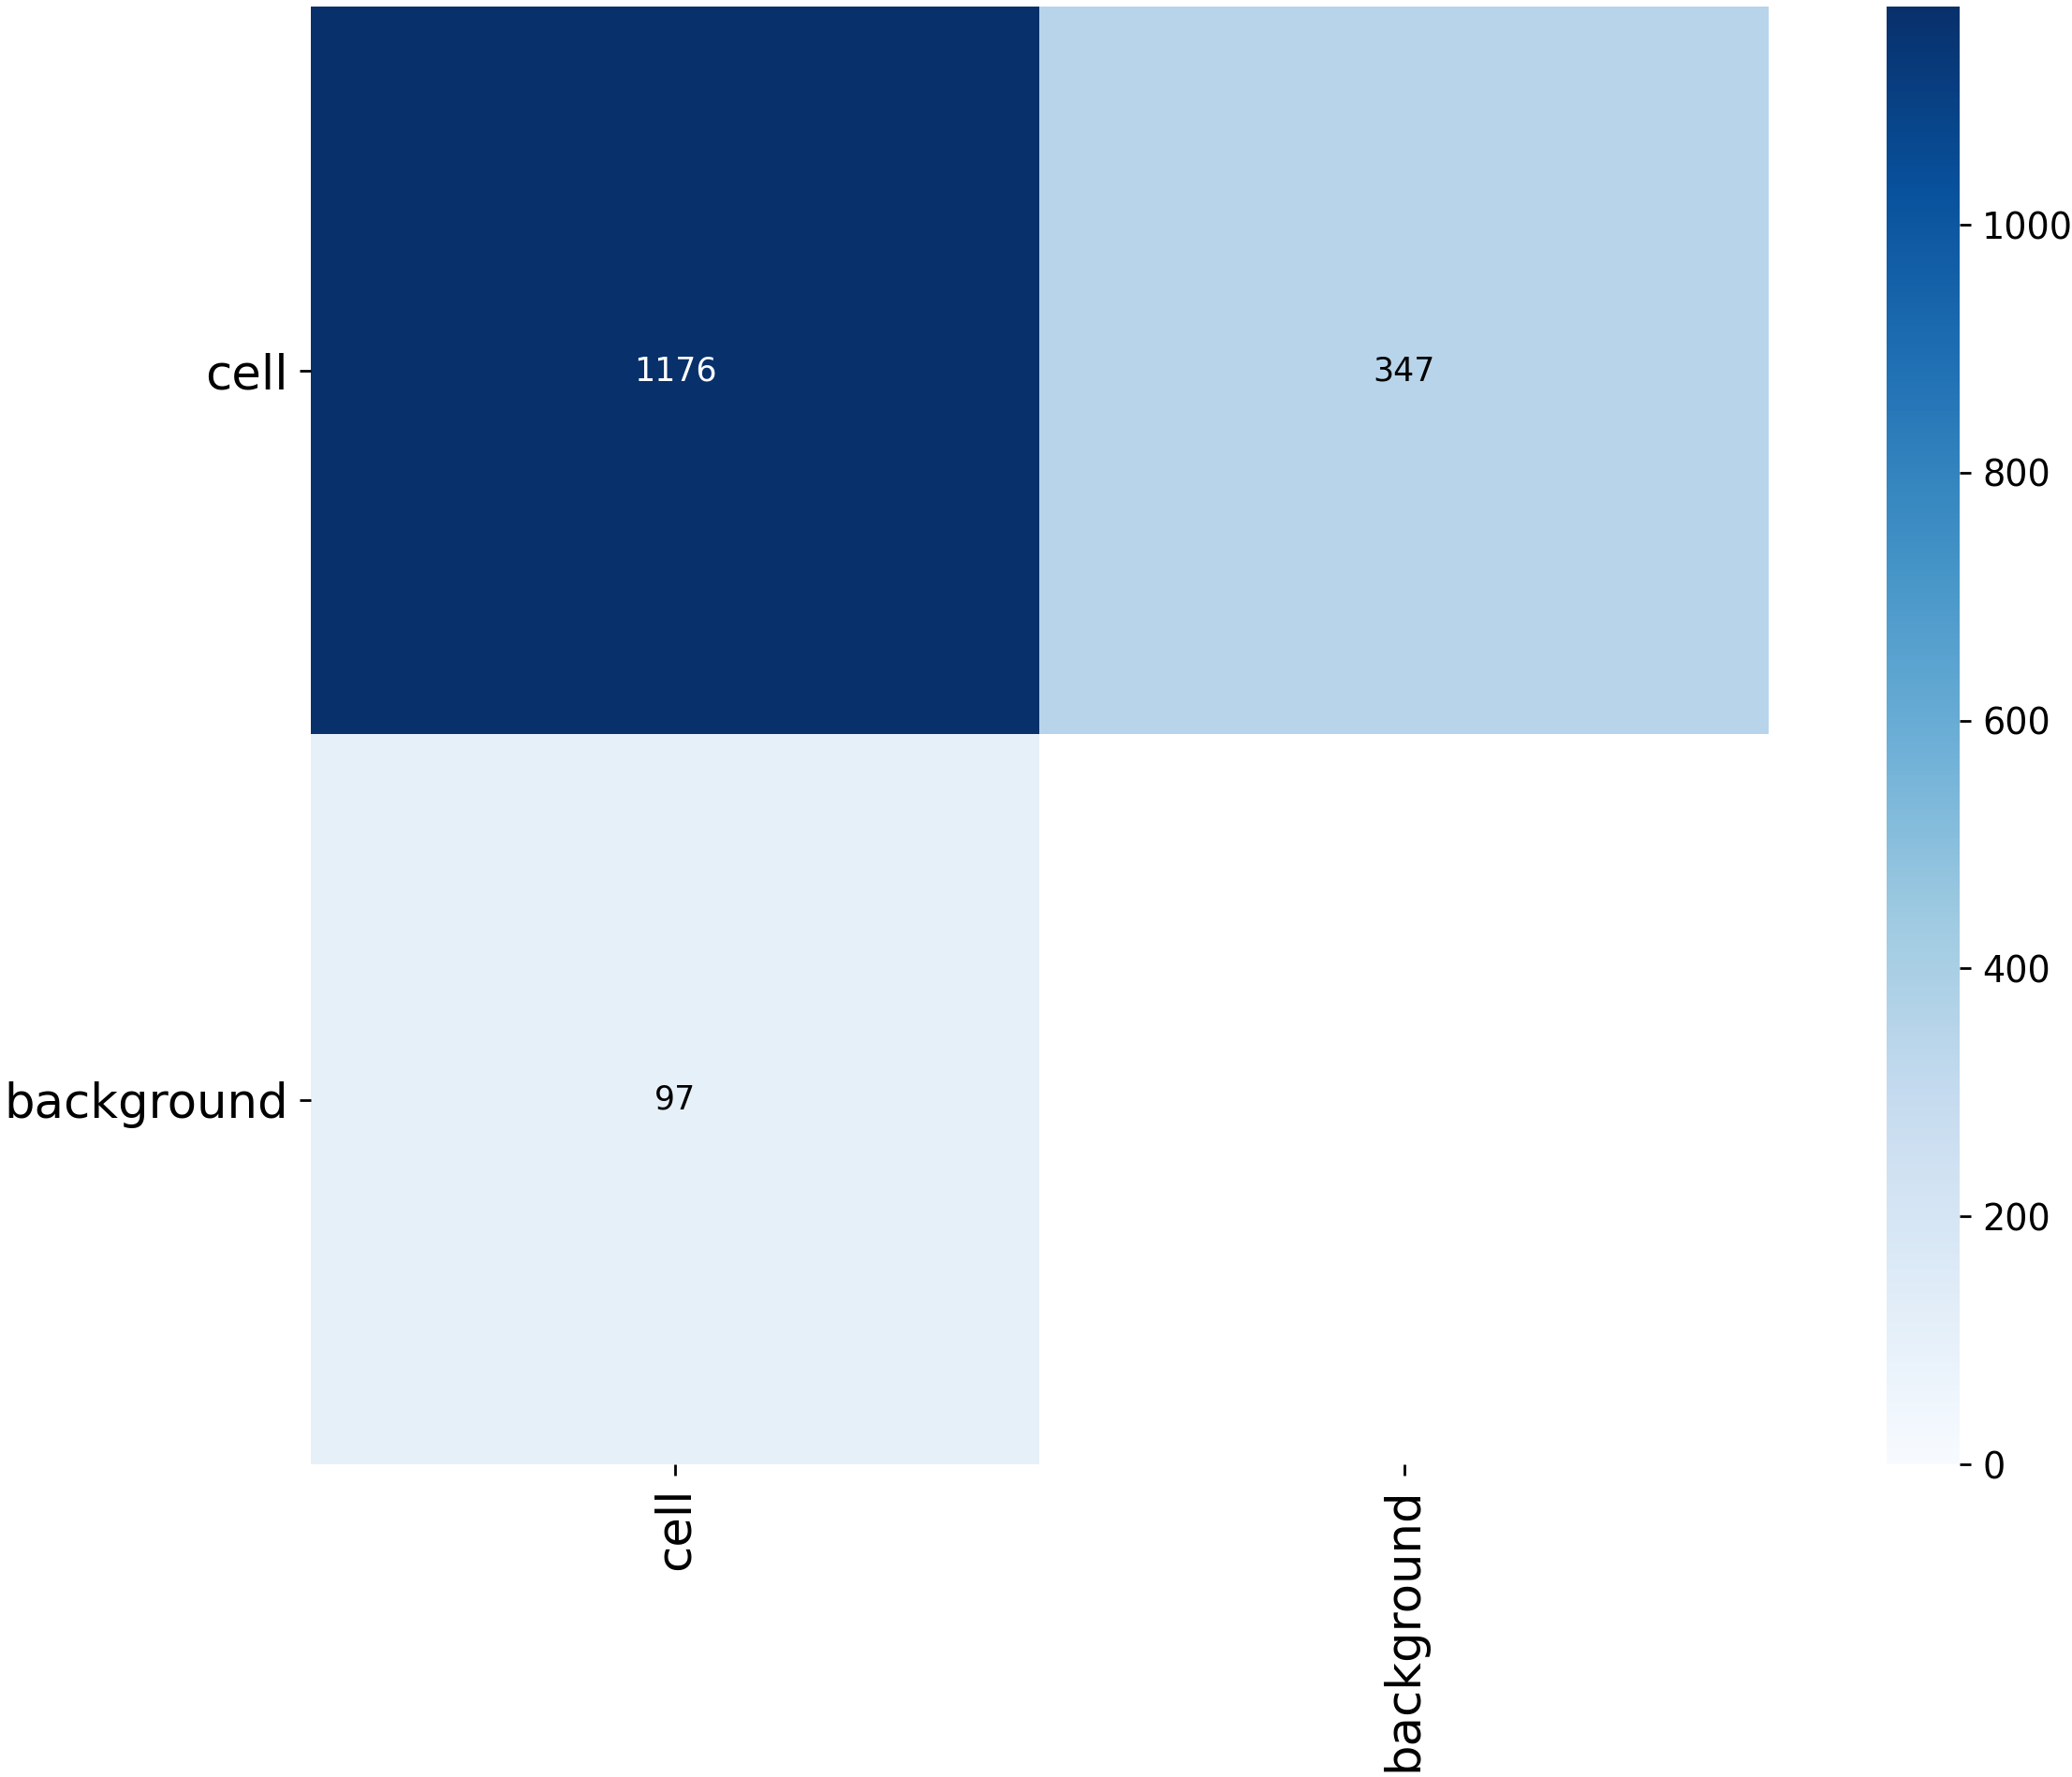
\includegraphics[height=5cm]{figuras/resultados experimentacion/yolov12l/original_test/confusion_matrix.png}
    \vspace{-0.3cm}
    \caption{\footnotesize YOLOv12l}
    \label{fig:confusion_yolov12l_original_test}
  \end{subfigure}
  
  \vspace{0.1cm}
  % Cuarta fila
  \begin{subfigure}[b]{0.45\textwidth}
    \centering
    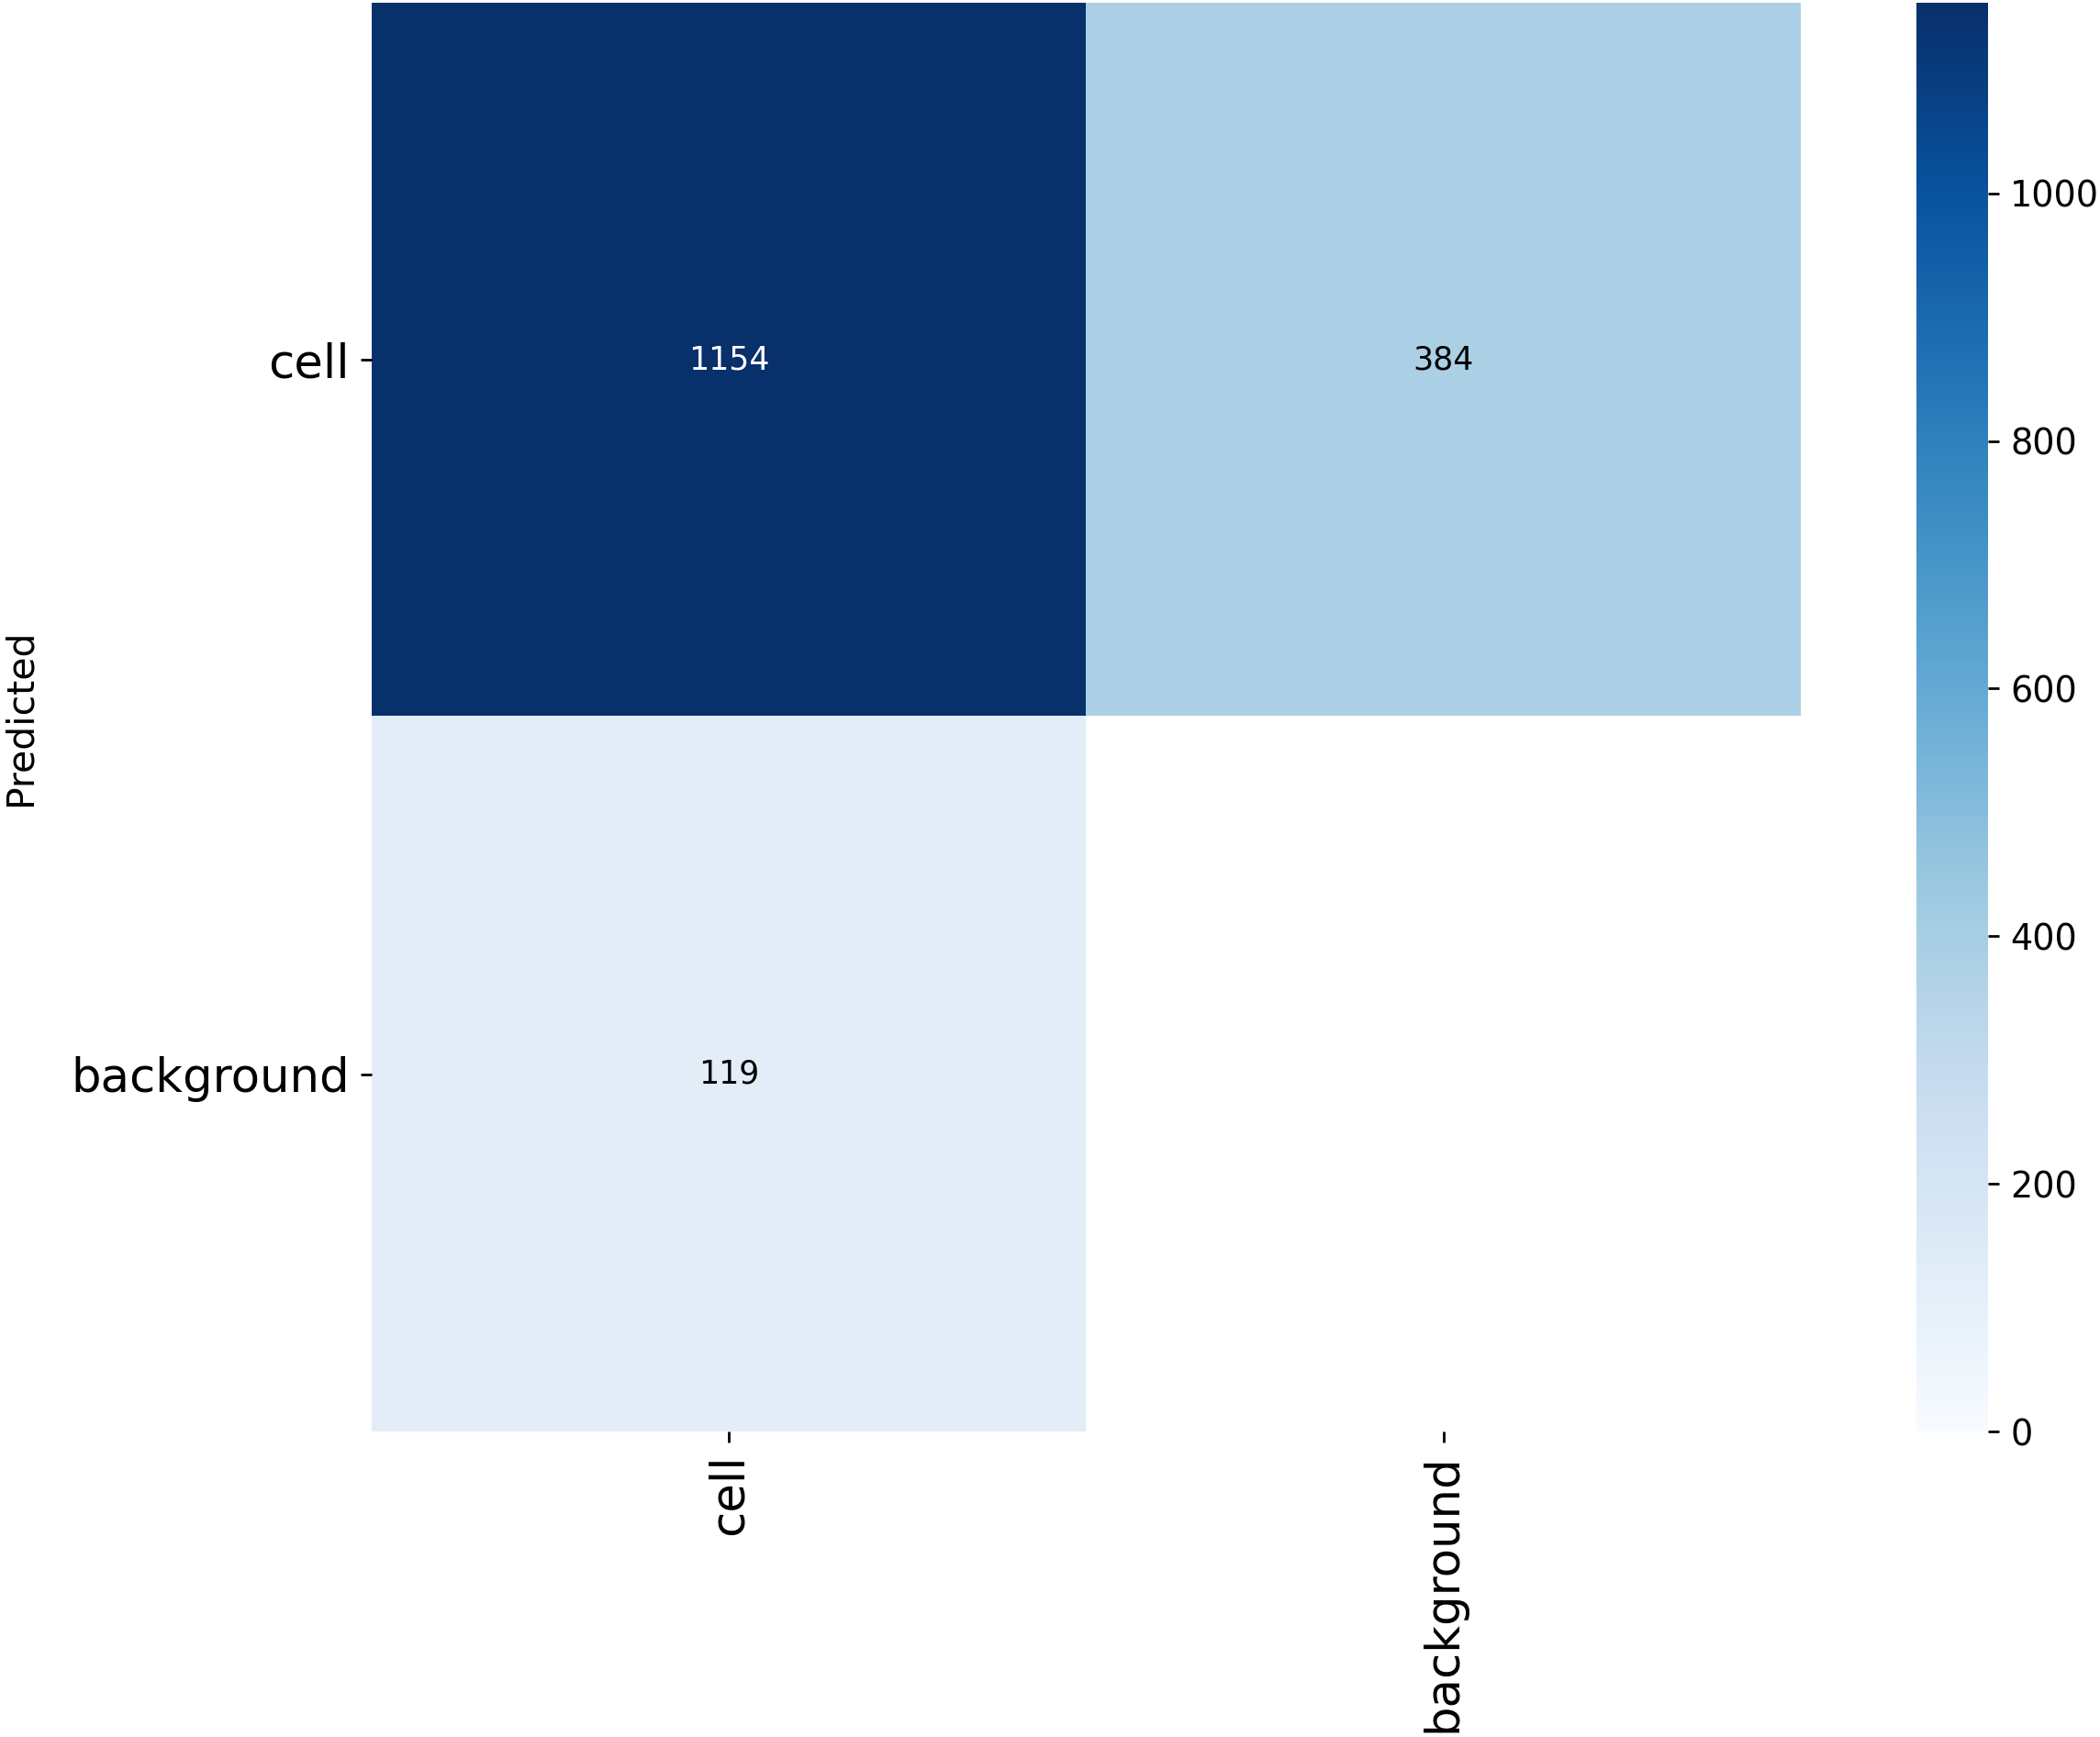
\includegraphics[height=5cm]{figuras/resultados experimentacion/custom/original_test/confusion_matrix.png}
    \vspace{-0.3cm}
    \caption{\footnotesize \textit{custom}}
    \label{fig:confusion_custom_original_test}
  \end{subfigure}
  \hfill
  \begin{subfigure}[b]{0.45\textwidth}
    \centering
    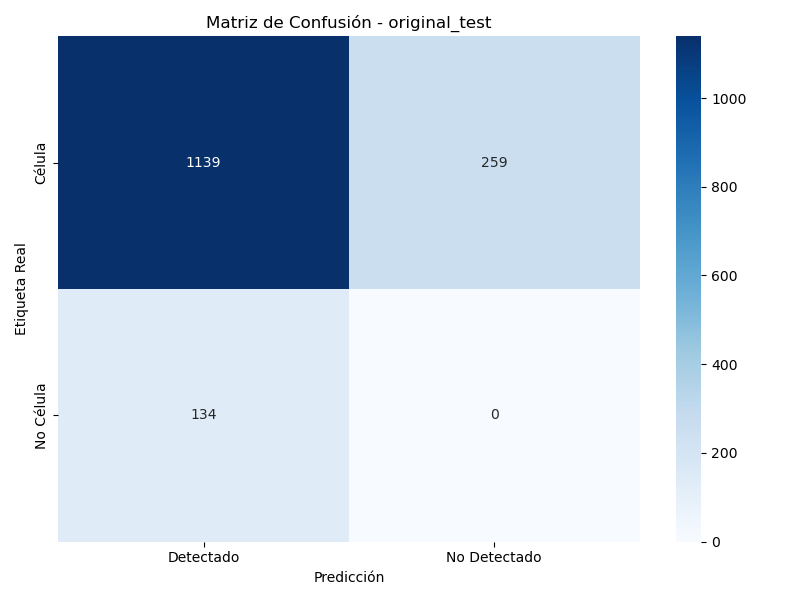
\includegraphics[height=5cm]{figuras/resultados experimentacion/ensemble/confusion_matrices/confusion_matrix_original_test.png}
    \vspace{-0.3cm}
    \caption{\footnotesize \textit{ensemble}}
    \label{fig:confusion_ensemble_original_test}
  \end{subfigure}
  
  \vspace{-0.2cm}
  \caption{Matrices de confusión para los modelos evaluados en original\_test}
  \label{fig:confusion_matrices_original_test}
\end{figure}


% FIGURA PARA TEST
\begin{figure}[H]
  \centering
  \vspace{-0.3cm}
  % Primera fila
  \begin{subfigure}[b]{0.45\textwidth}
    \centering
    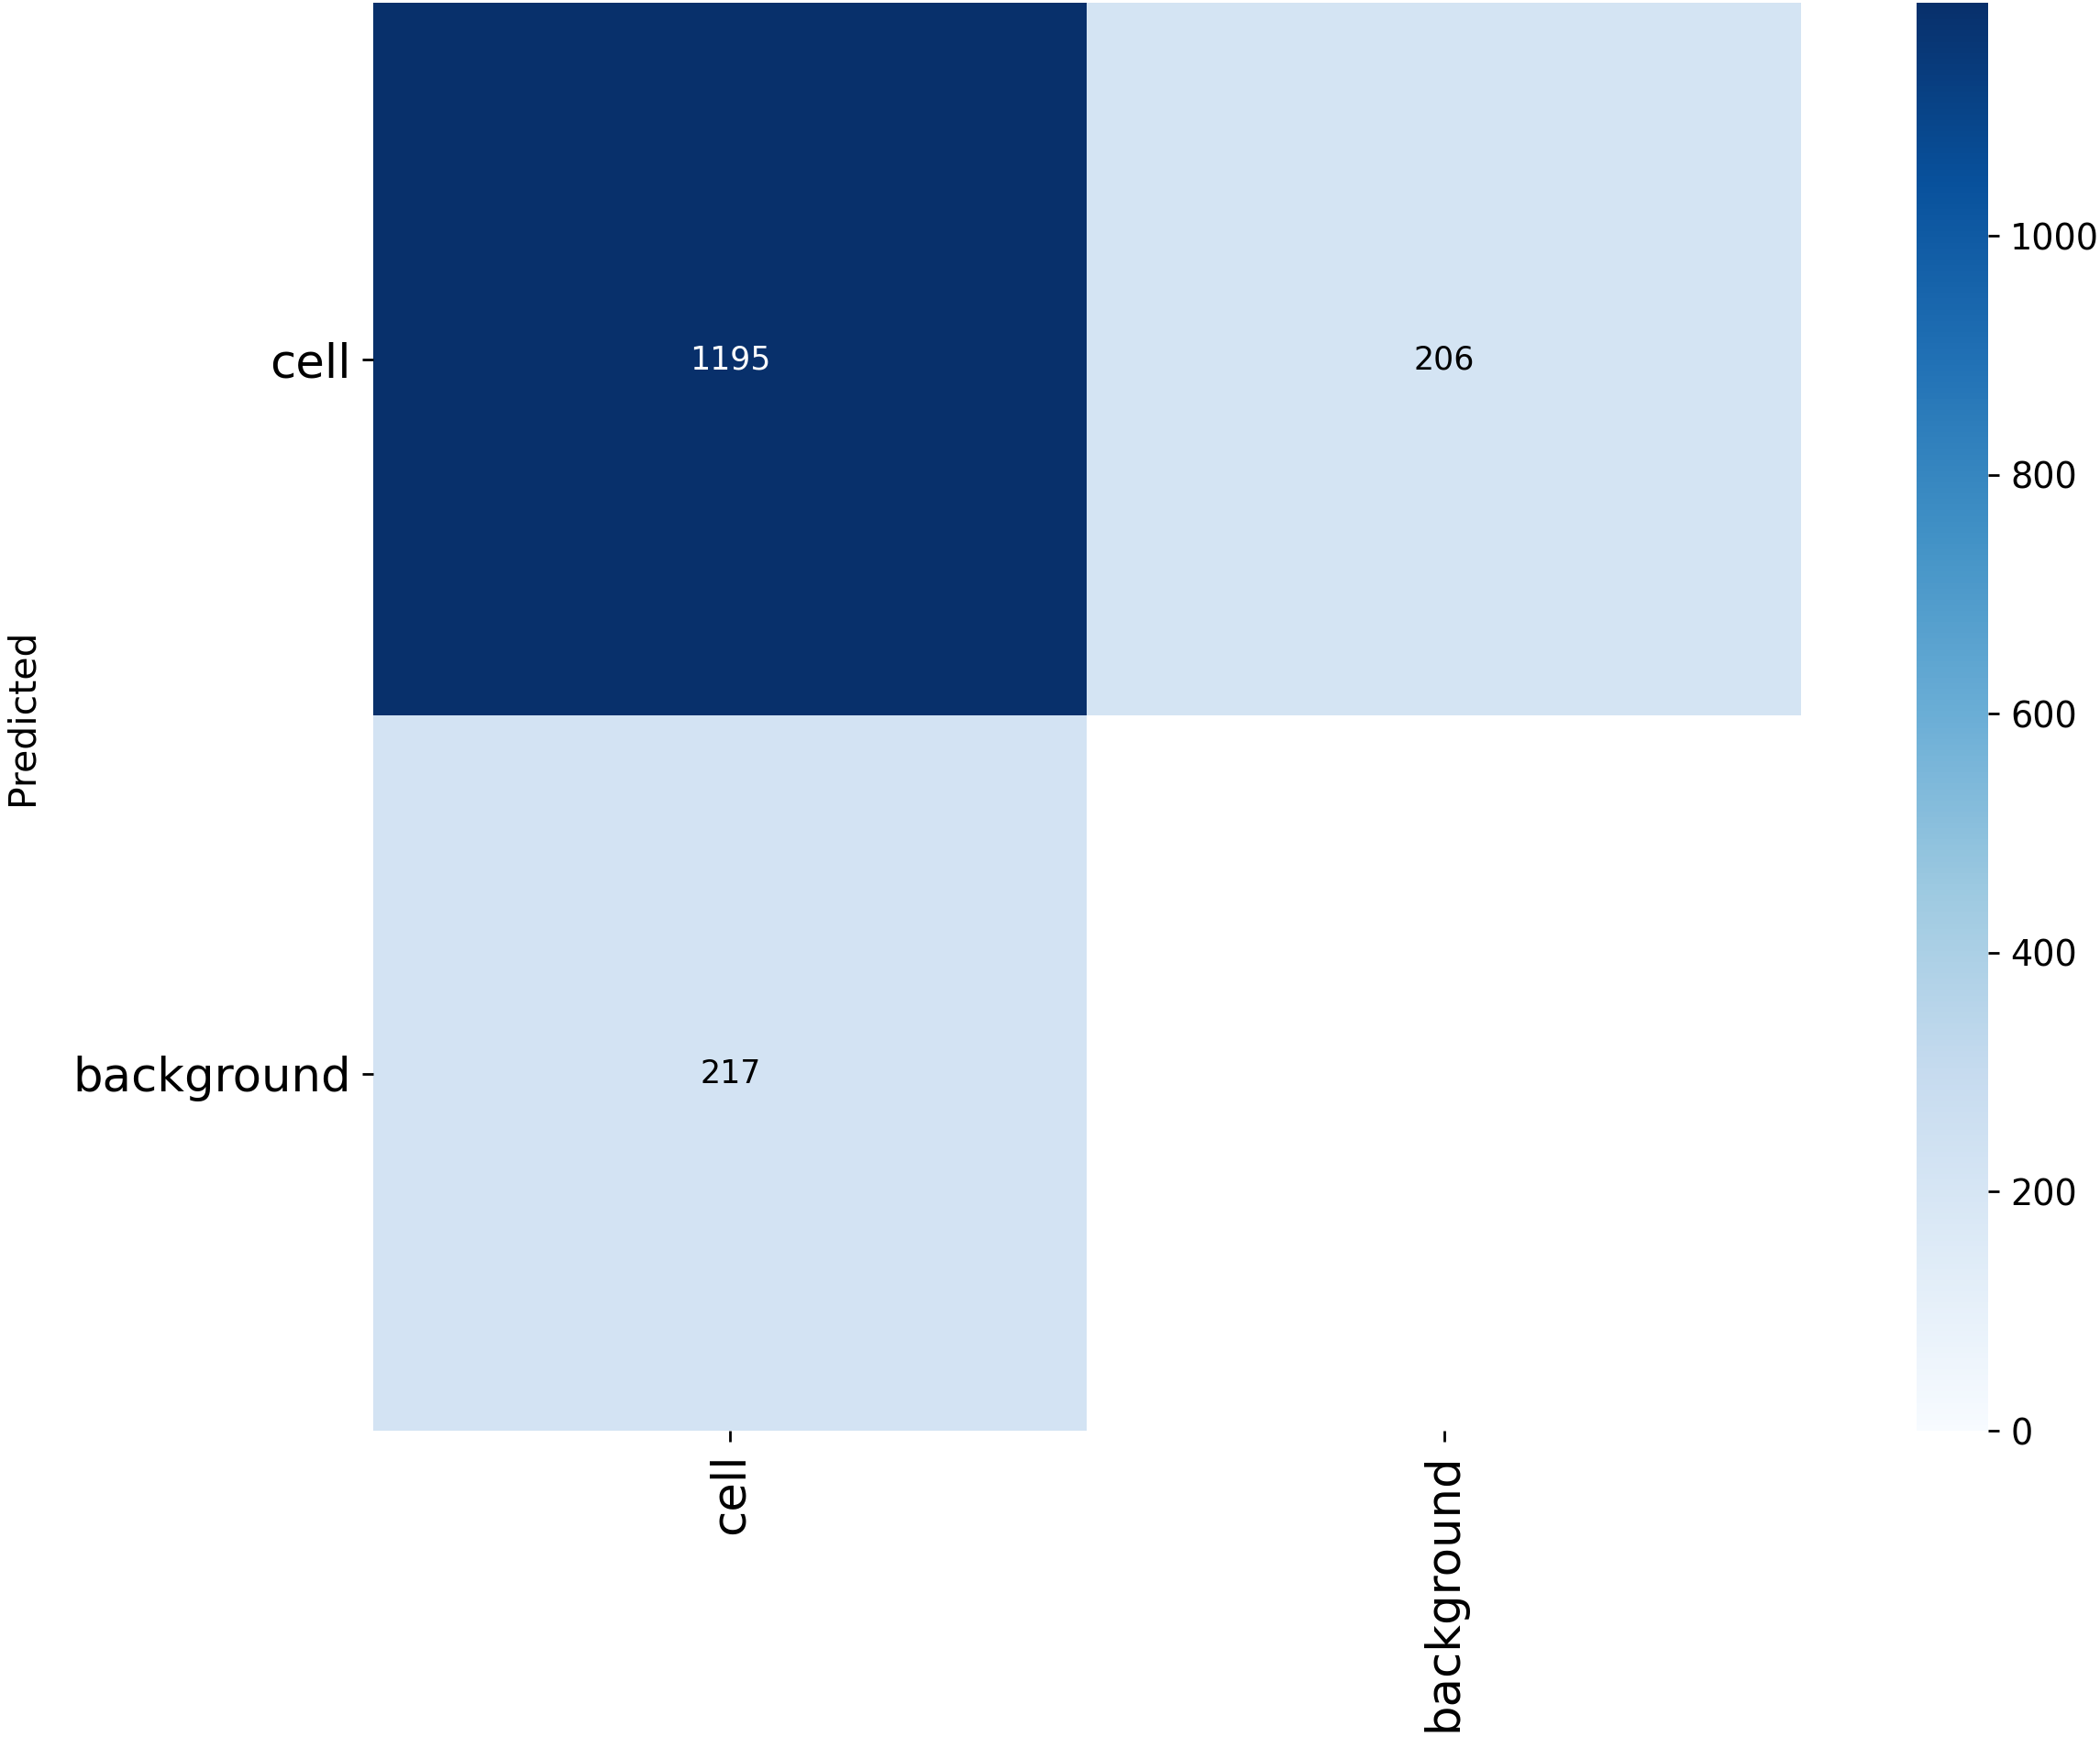
\includegraphics[height=5cm]{figuras/resultados experimentacion/yolov8s/test/confusion_matrix.png}
    \vspace{-0.3cm}
    \caption{\footnotesize YOLOv8s}
    \label{fig:confusion_yolov8s_test}
  \end{subfigure}
  \hfill
  \begin{subfigure}[b]{0.45\textwidth}
    \centering
    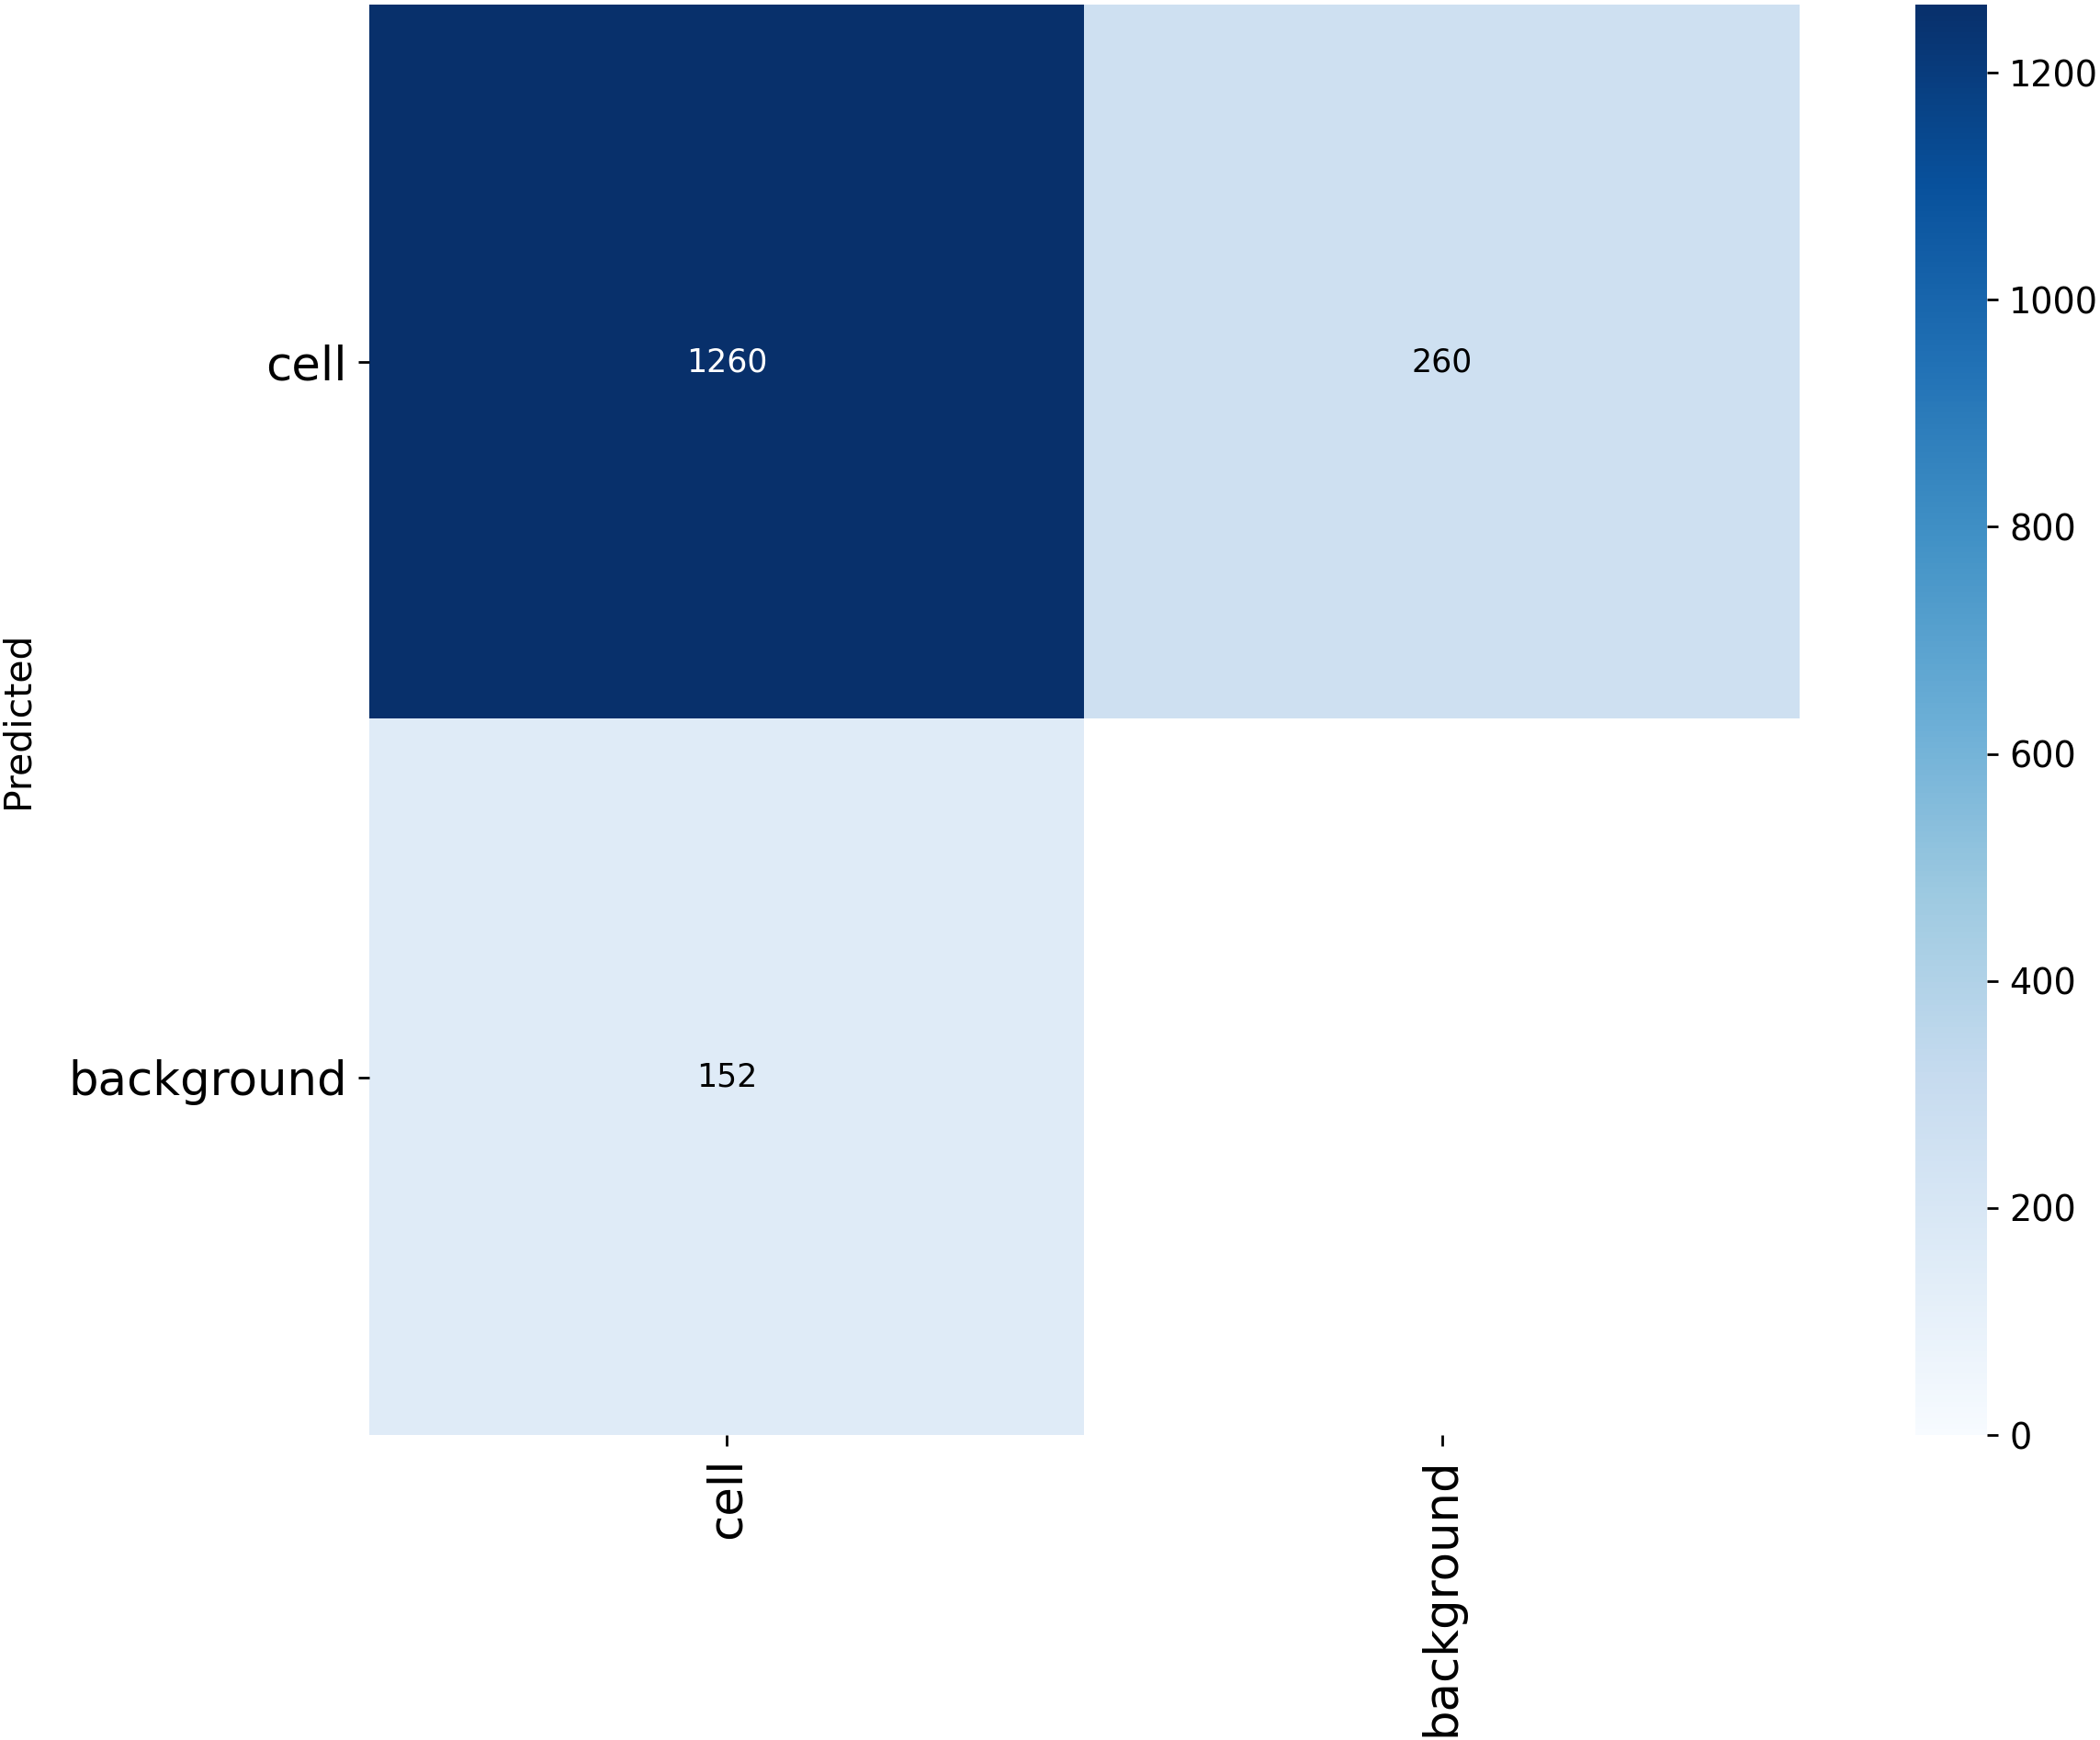
\includegraphics[height=5cm]{figuras/resultados experimentacion/yolov9s/test/confusion_matrix.png}
    \vspace{-0.3cm}
    \caption{\footnotesize YOLOv9s}
    \label{fig:confusion_yolov9s_test}
  \end{subfigure}
  
  \vspace{0.1cm}
  % Segunda fila
  \begin{subfigure}[b]{0.45\textwidth}
    \centering
    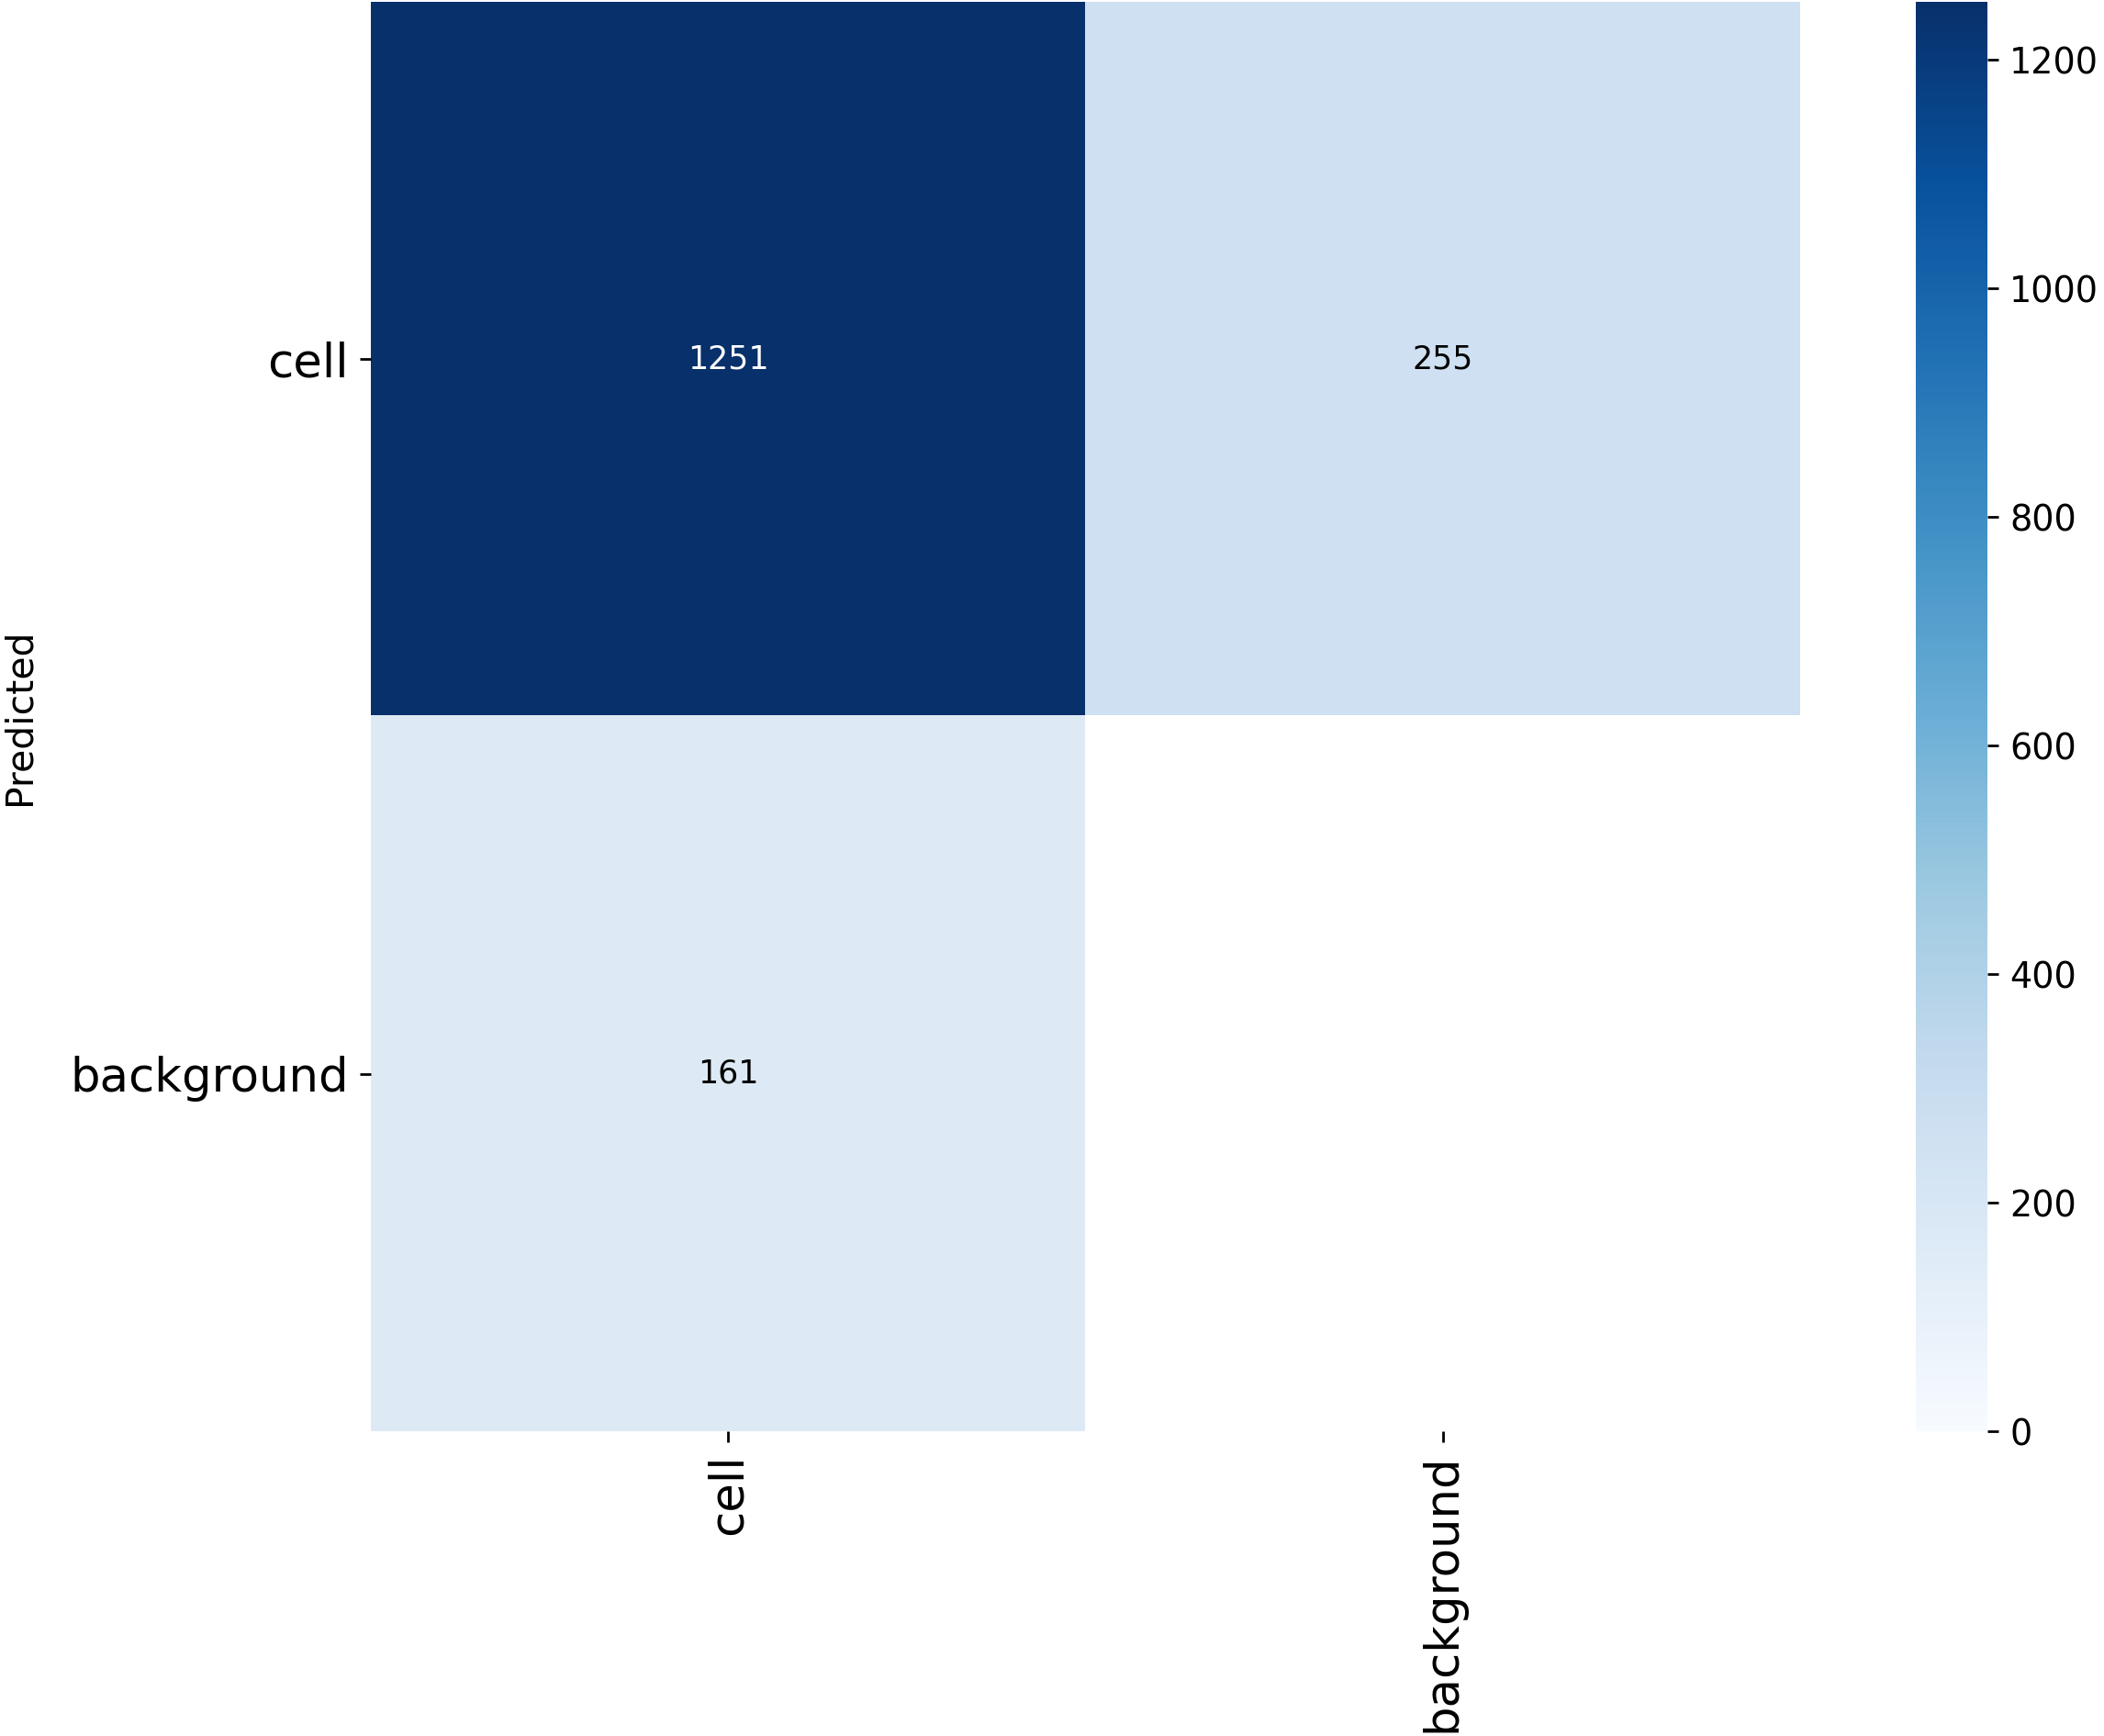
\includegraphics[height=5cm]{figuras/resultados experimentacion/yolov10s/test/confusion_matrix.png}
    \vspace{-0.3cm}
    \caption{\footnotesize YOLOv10s}
    \label{fig:confusion_yolov10s_test}
  \end{subfigure}
  \hfill
  \begin{subfigure}[b]{0.45\textwidth}
    \centering
    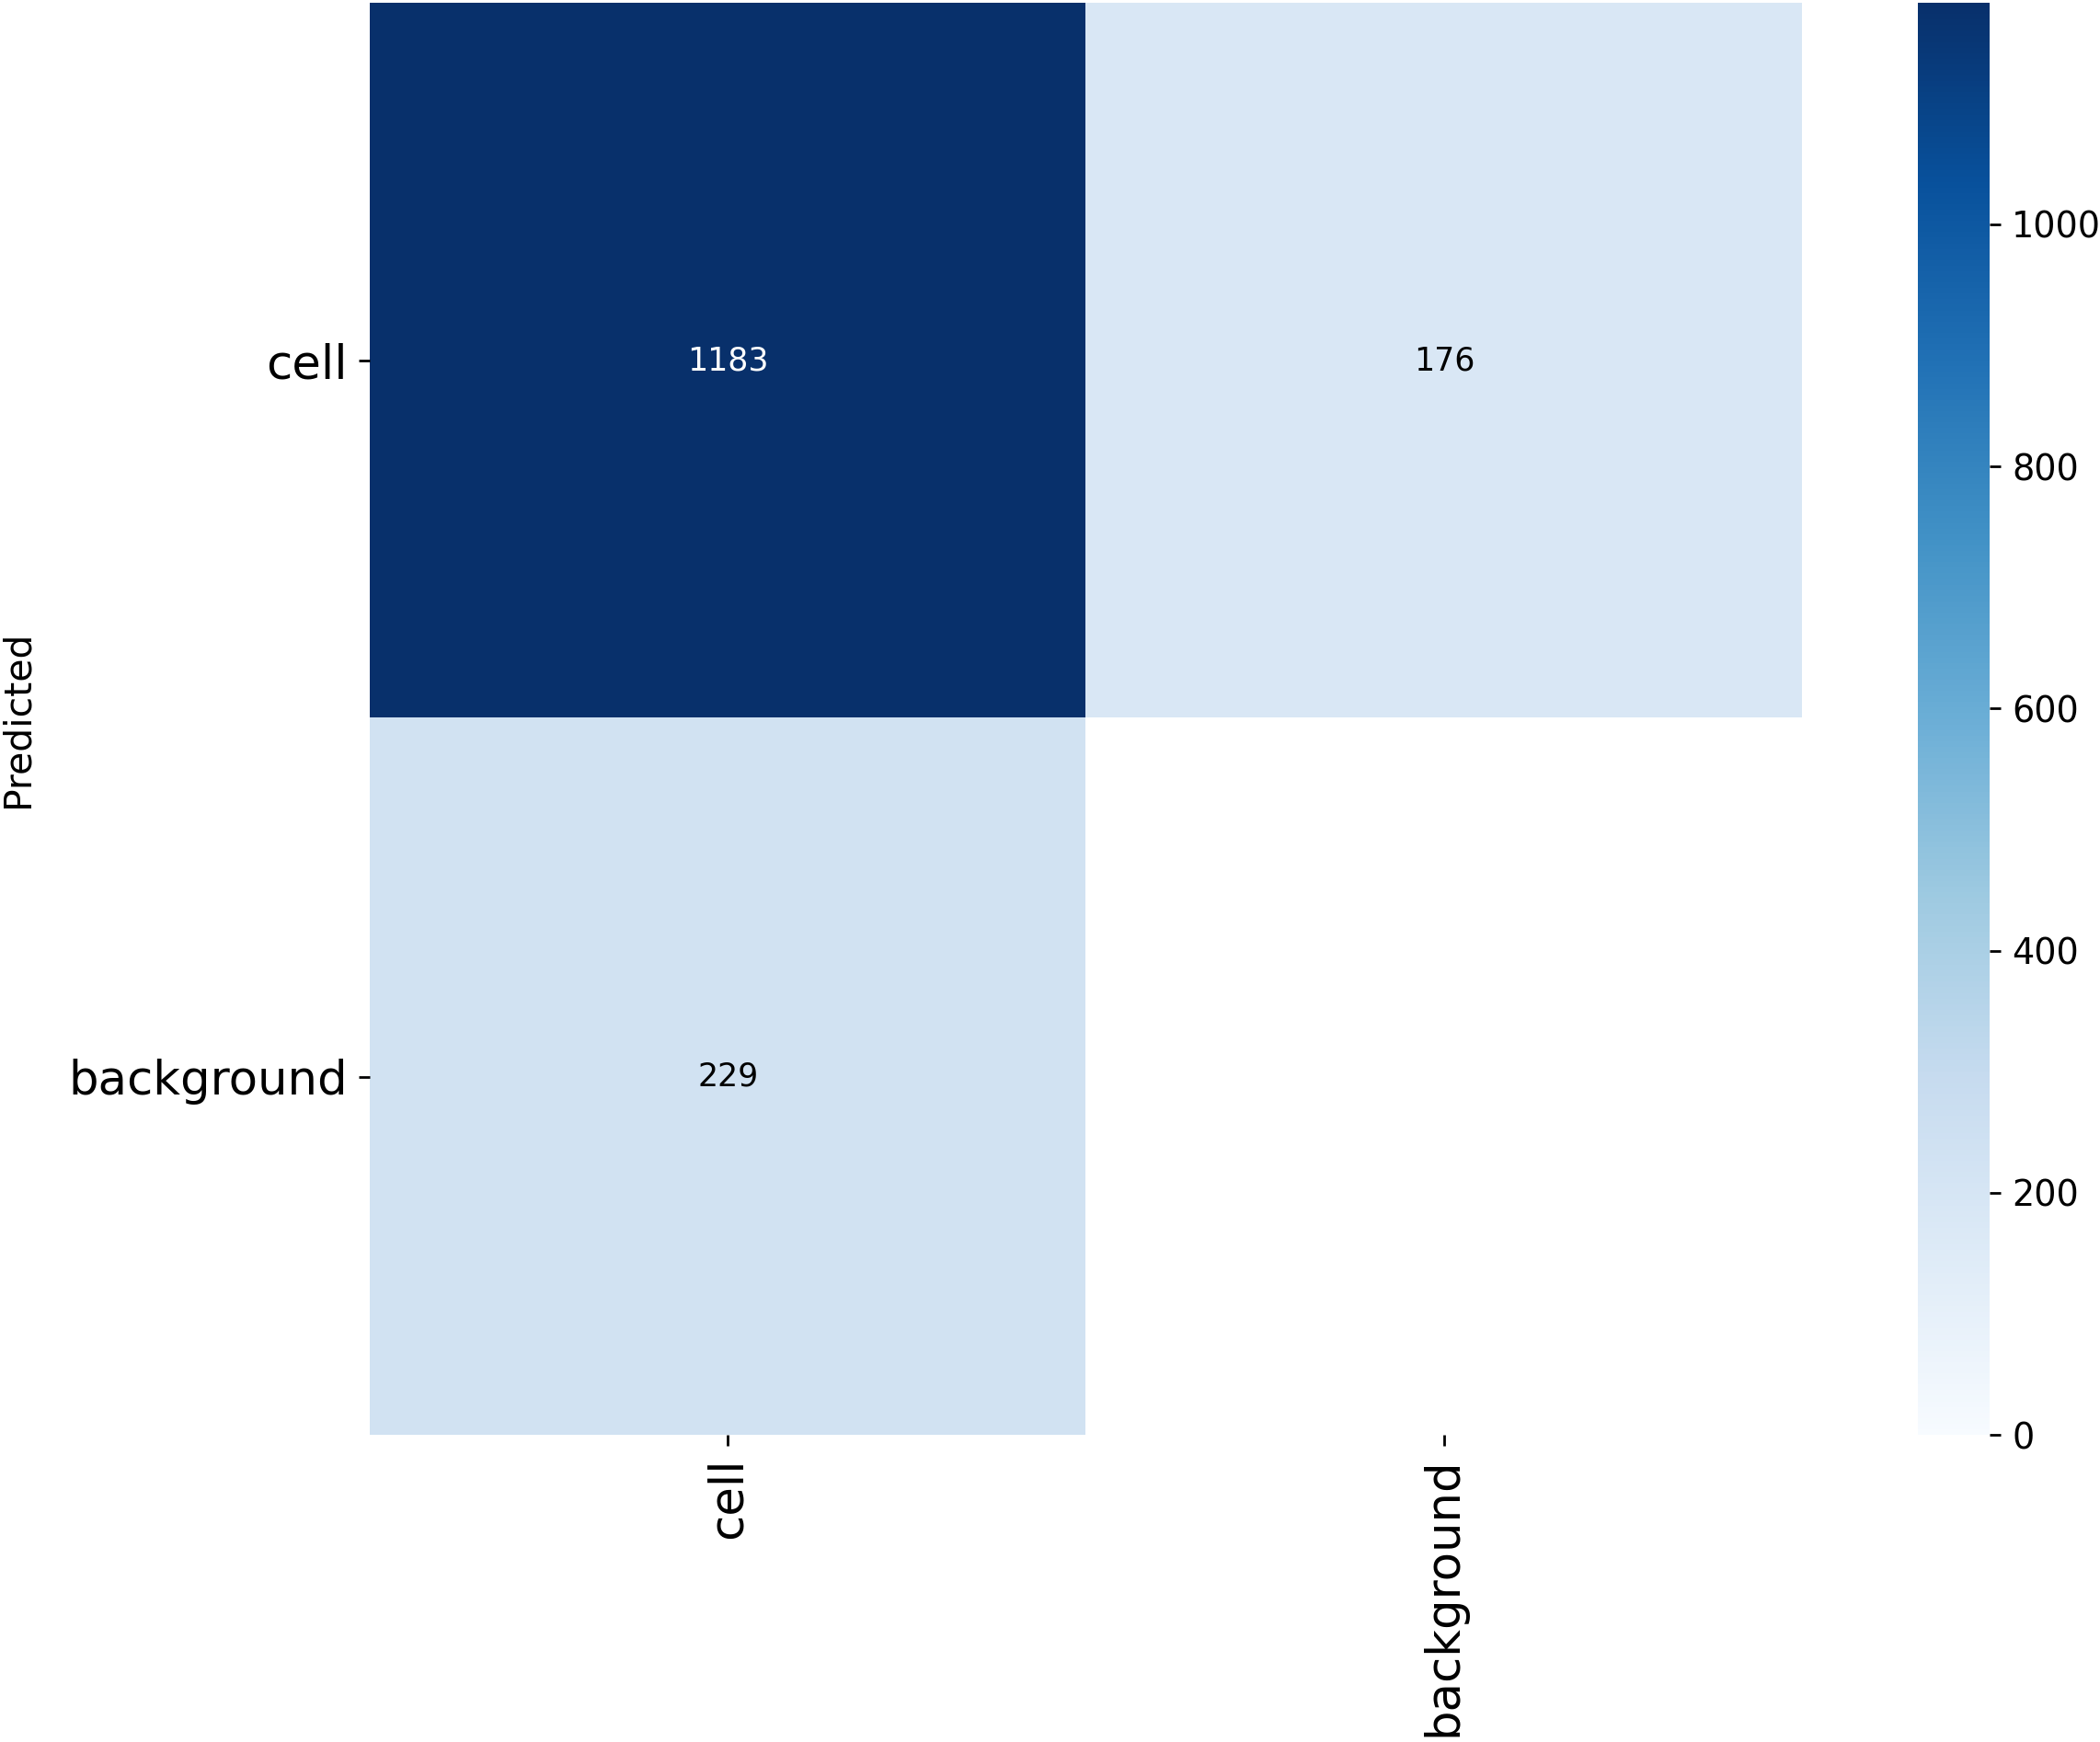
\includegraphics[height=5cm]{figuras/resultados experimentacion/yolov11s/test/confusion_matrix.png}
    \vspace{-0.3cm}
    \caption{\footnotesize YOLOv11s}
    \label{fig:confusion_yolov11s_test}
  \end{subfigure}
  
  \vspace{0.1cm}
  % Tercera fila
  \begin{subfigure}[b]{0.45\textwidth}
    \centering
    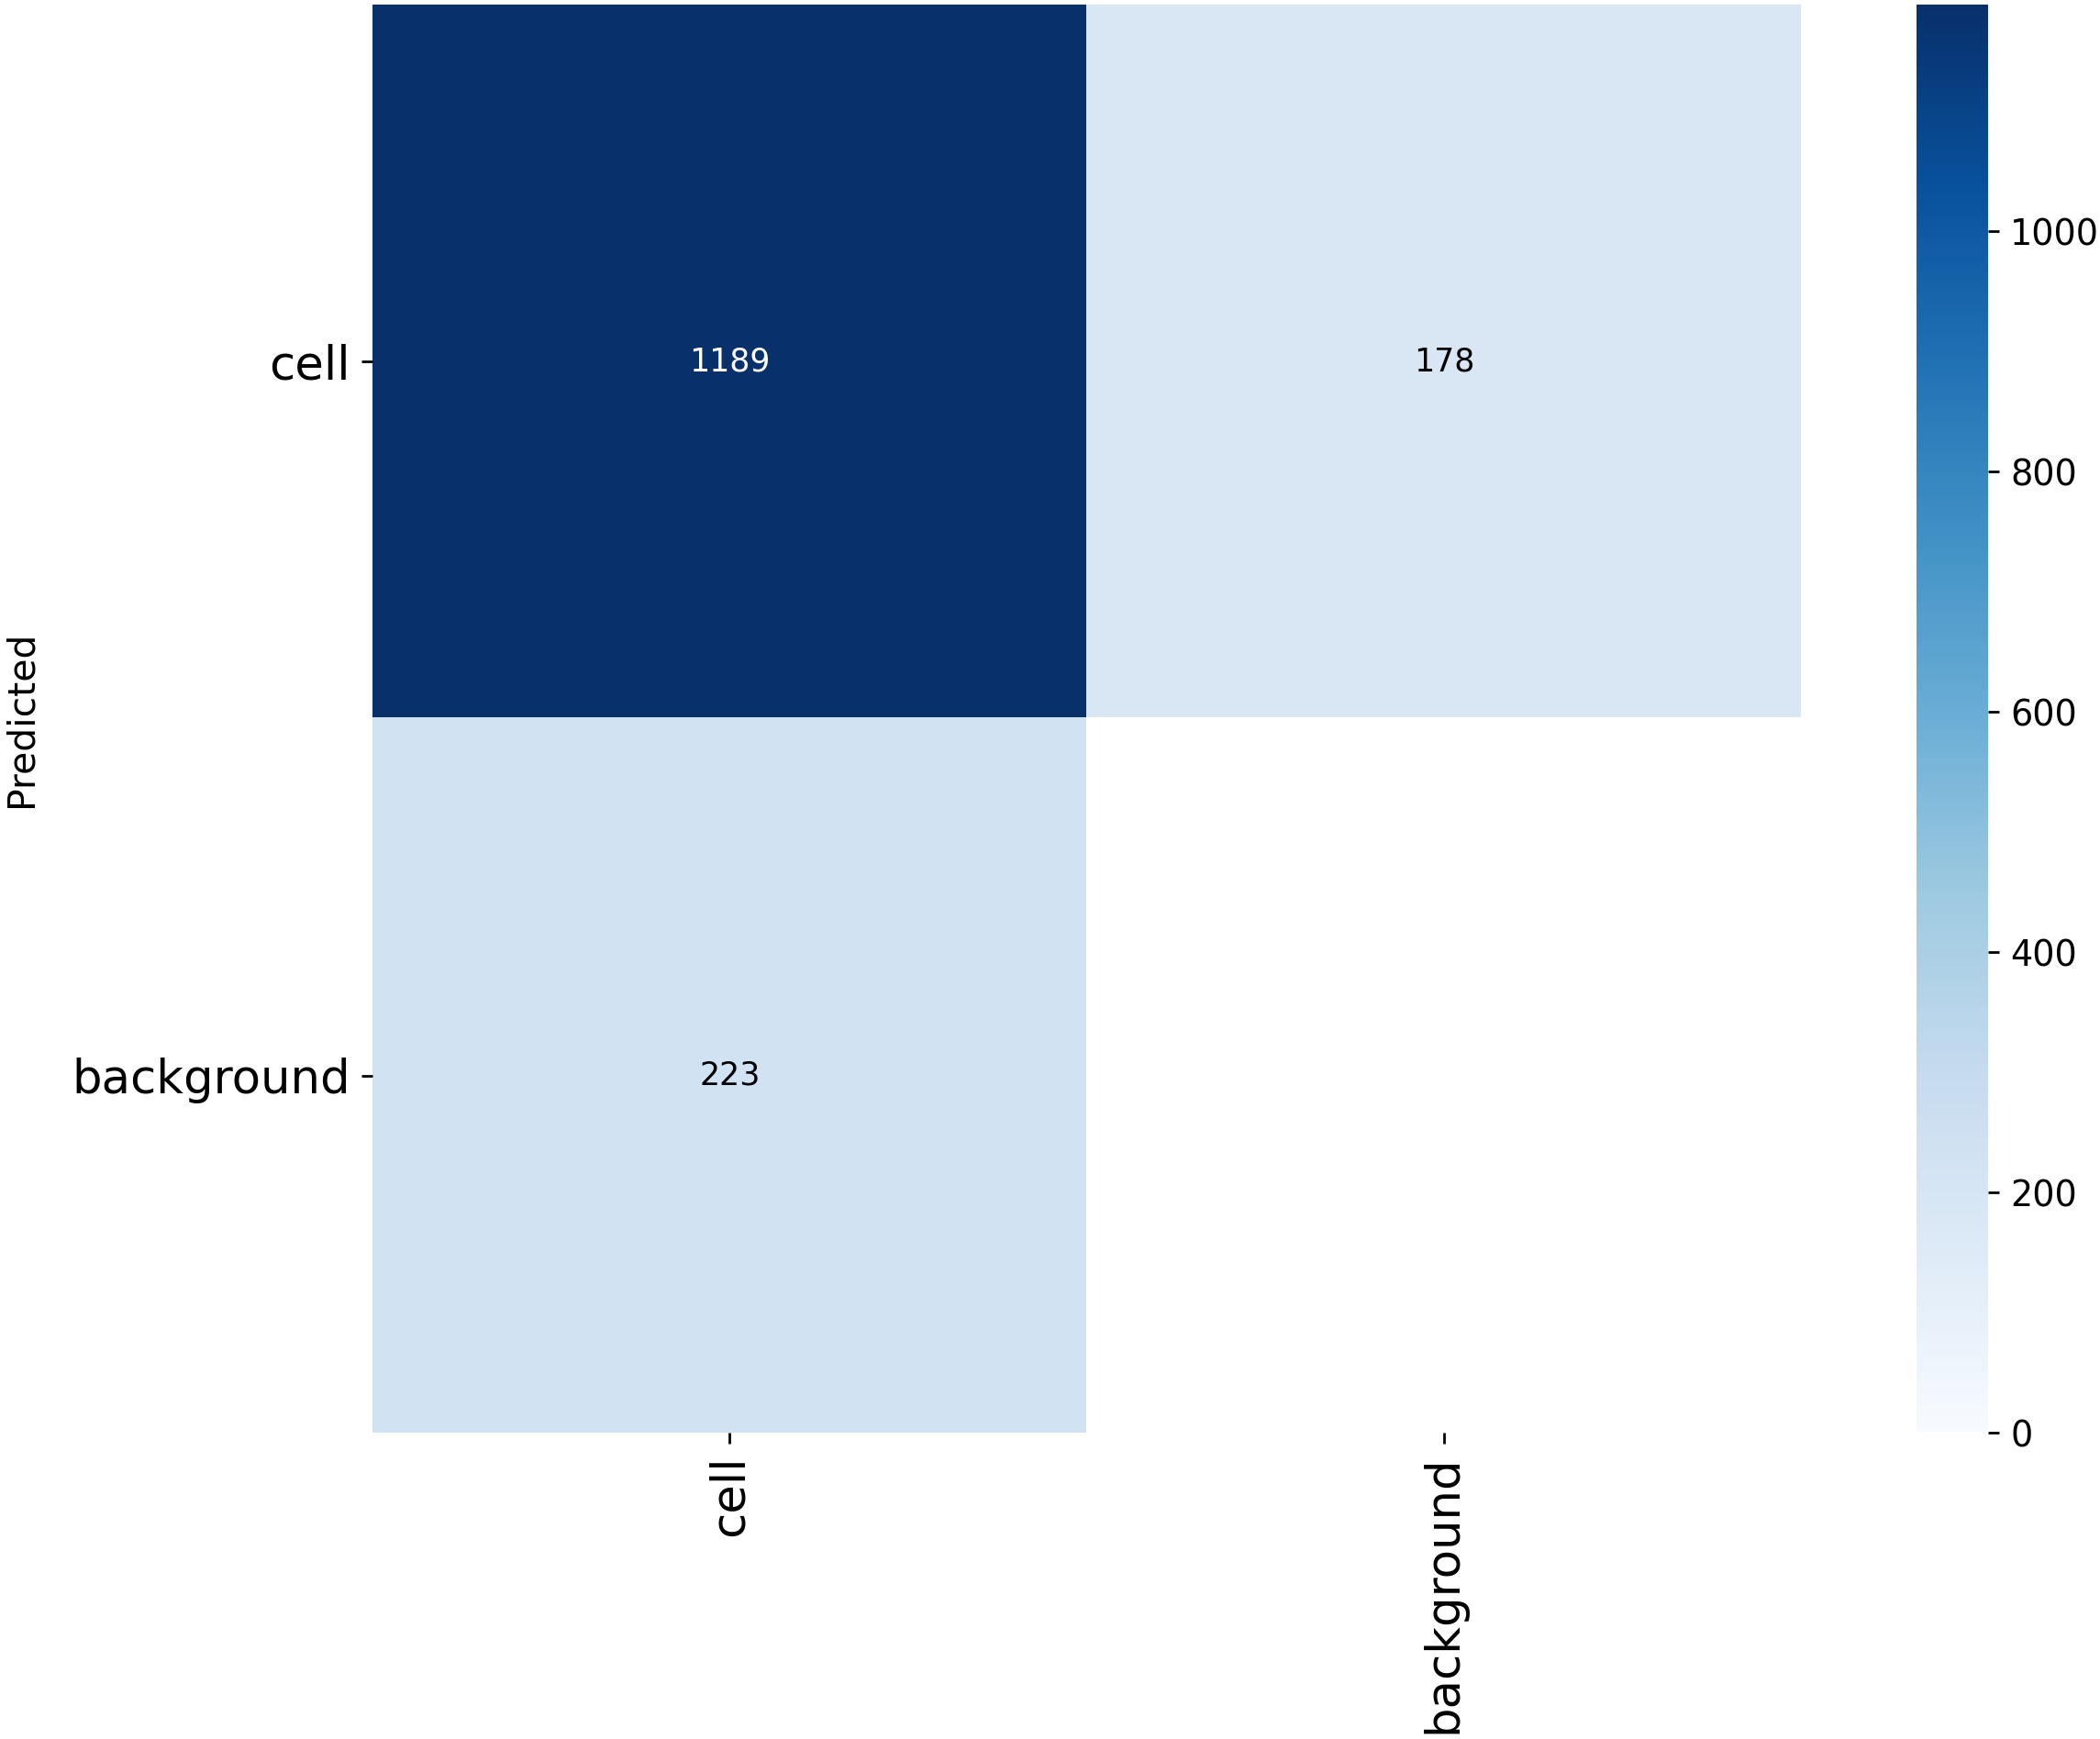
\includegraphics[height=5cm]{figuras/resultados experimentacion/yolov12s/test/confusion_matrix.png}
    \vspace{-0.3cm}
    \caption{\footnotesize YOLOv12s}
    \label{fig:confusion_yolov12s_test}
  \end{subfigure}
  \hfill
  \begin{subfigure}[b]{0.45\textwidth}
    \centering
    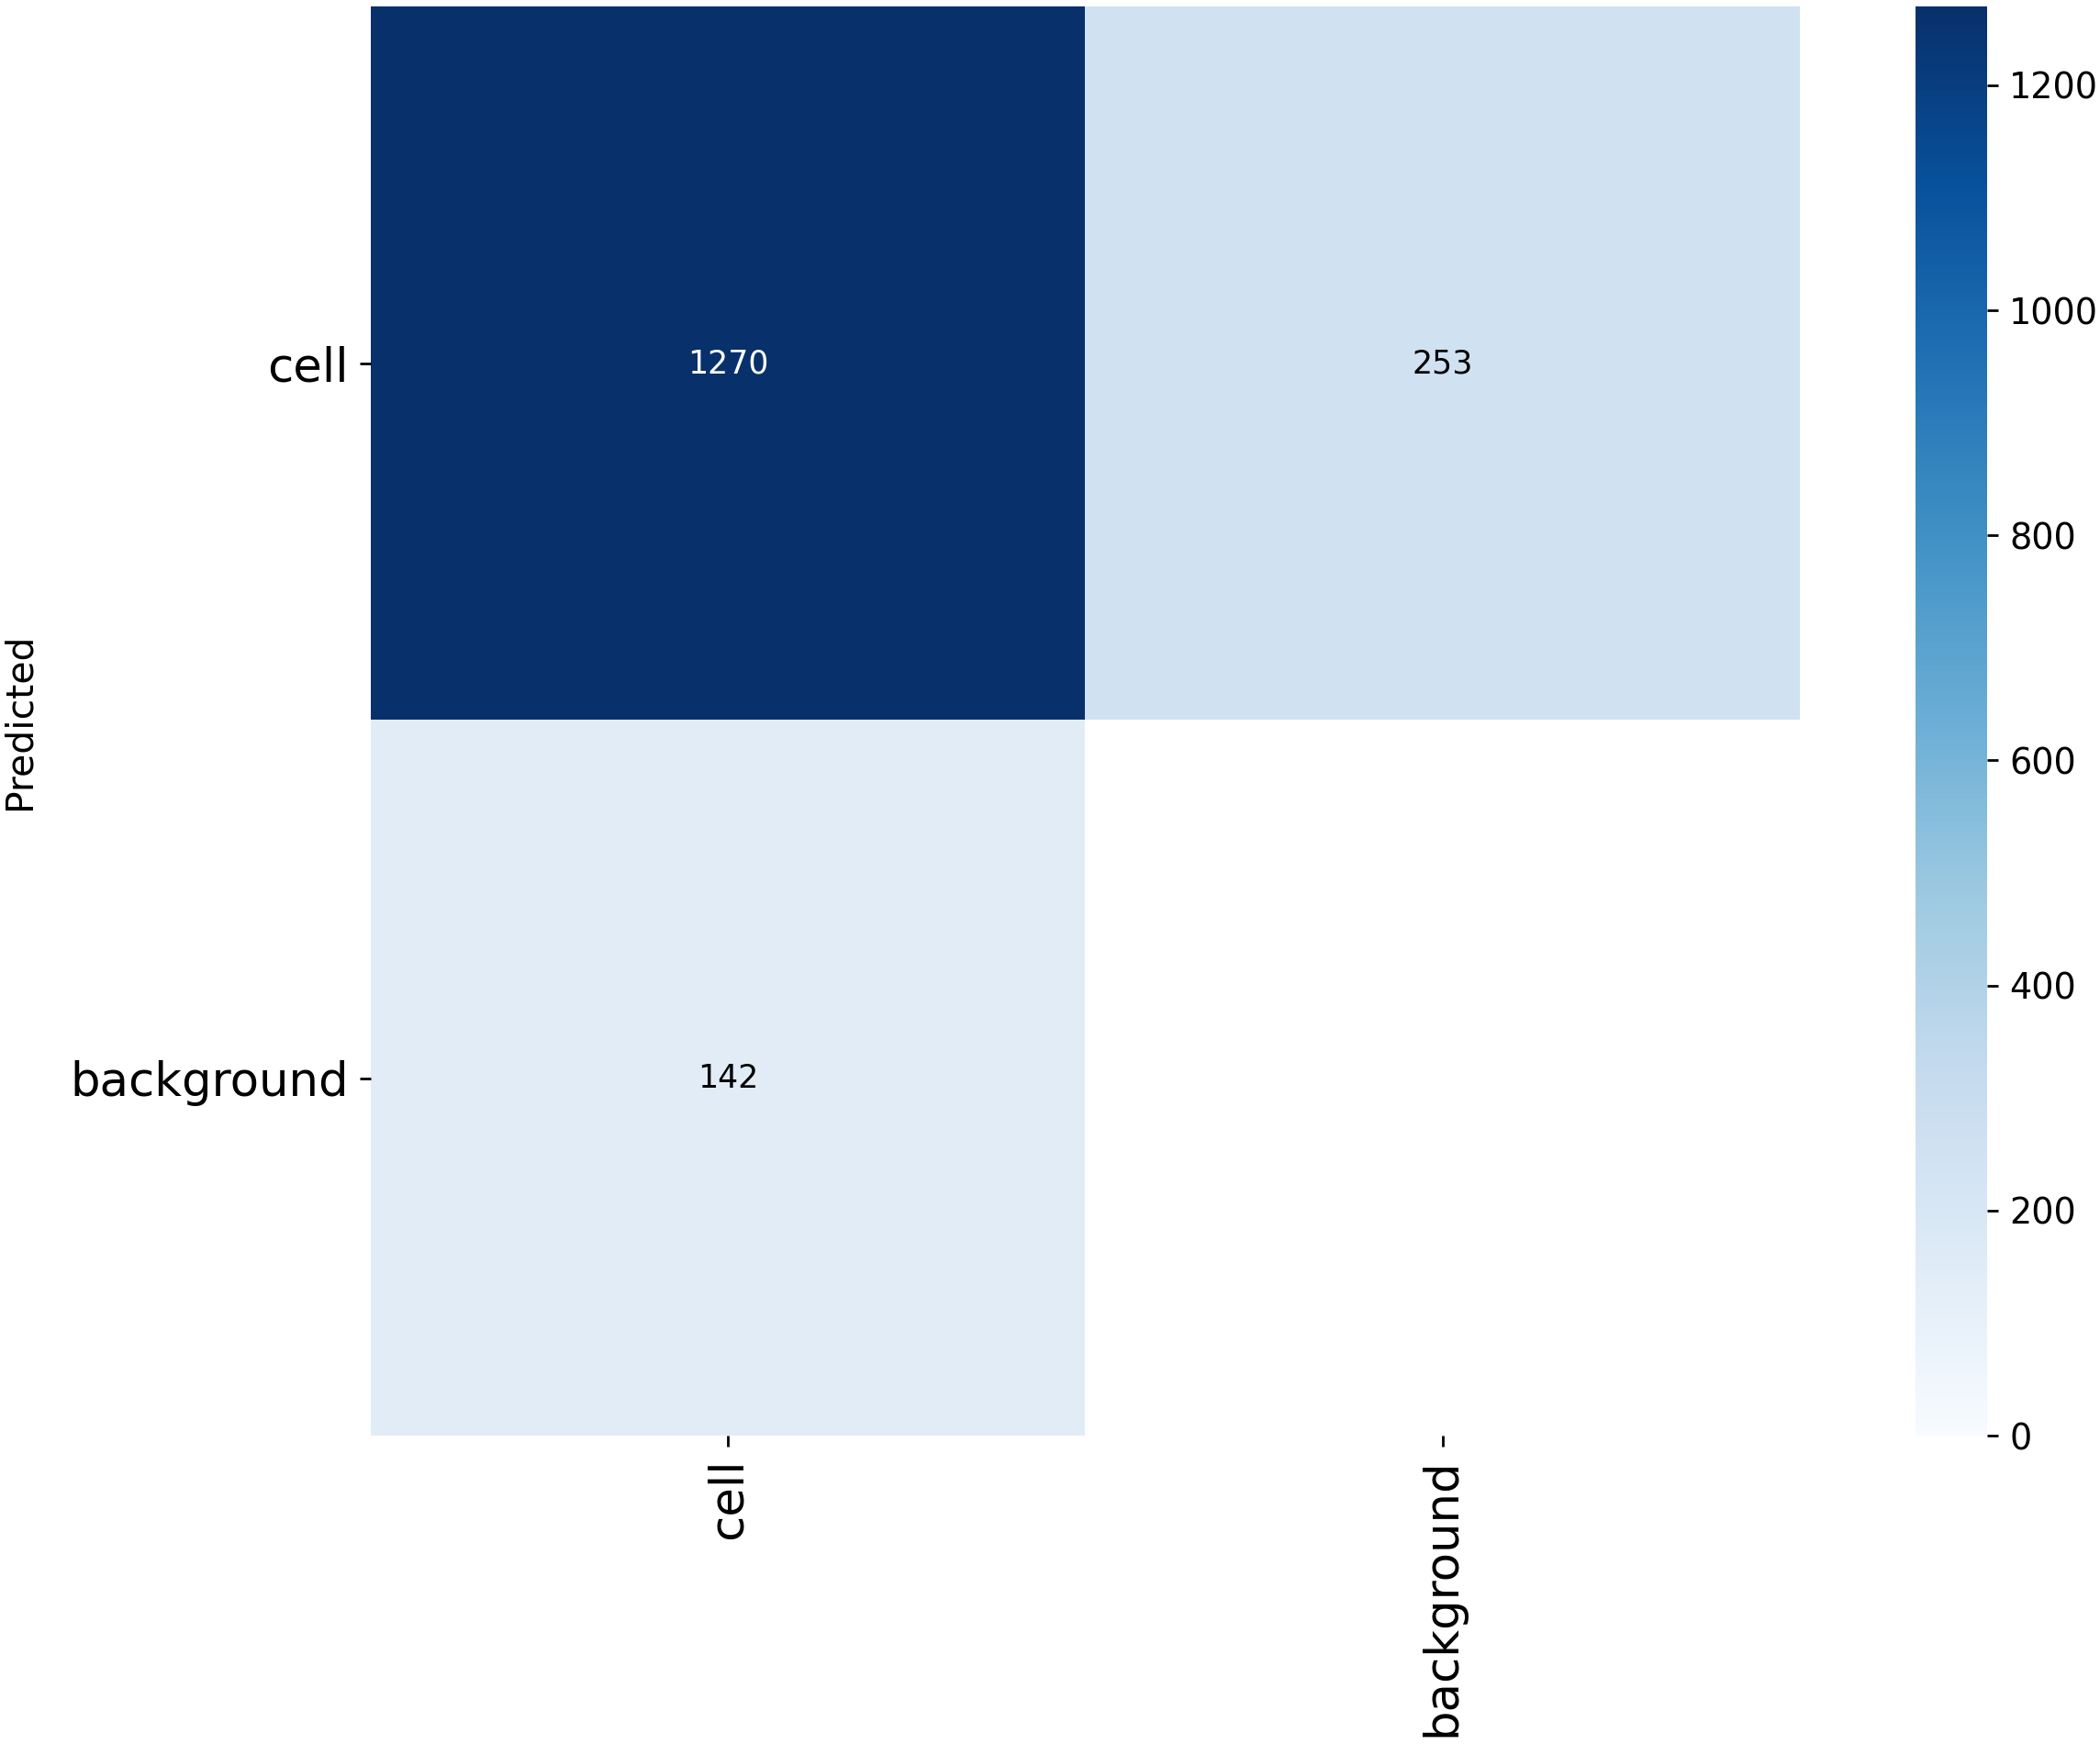
\includegraphics[height=5cm]{figuras/resultados experimentacion/yolov12l/test/confusion_matrix.png}
    \vspace{-0.3cm}
    \caption{\footnotesize YOLOv12l}
    \label{fig:confusion_yolov12l_test}
  \end{subfigure}
  
  \vspace{0.1cm}
  % Cuarta fila
  \begin{subfigure}[b]{0.45\textwidth}
    \centering
    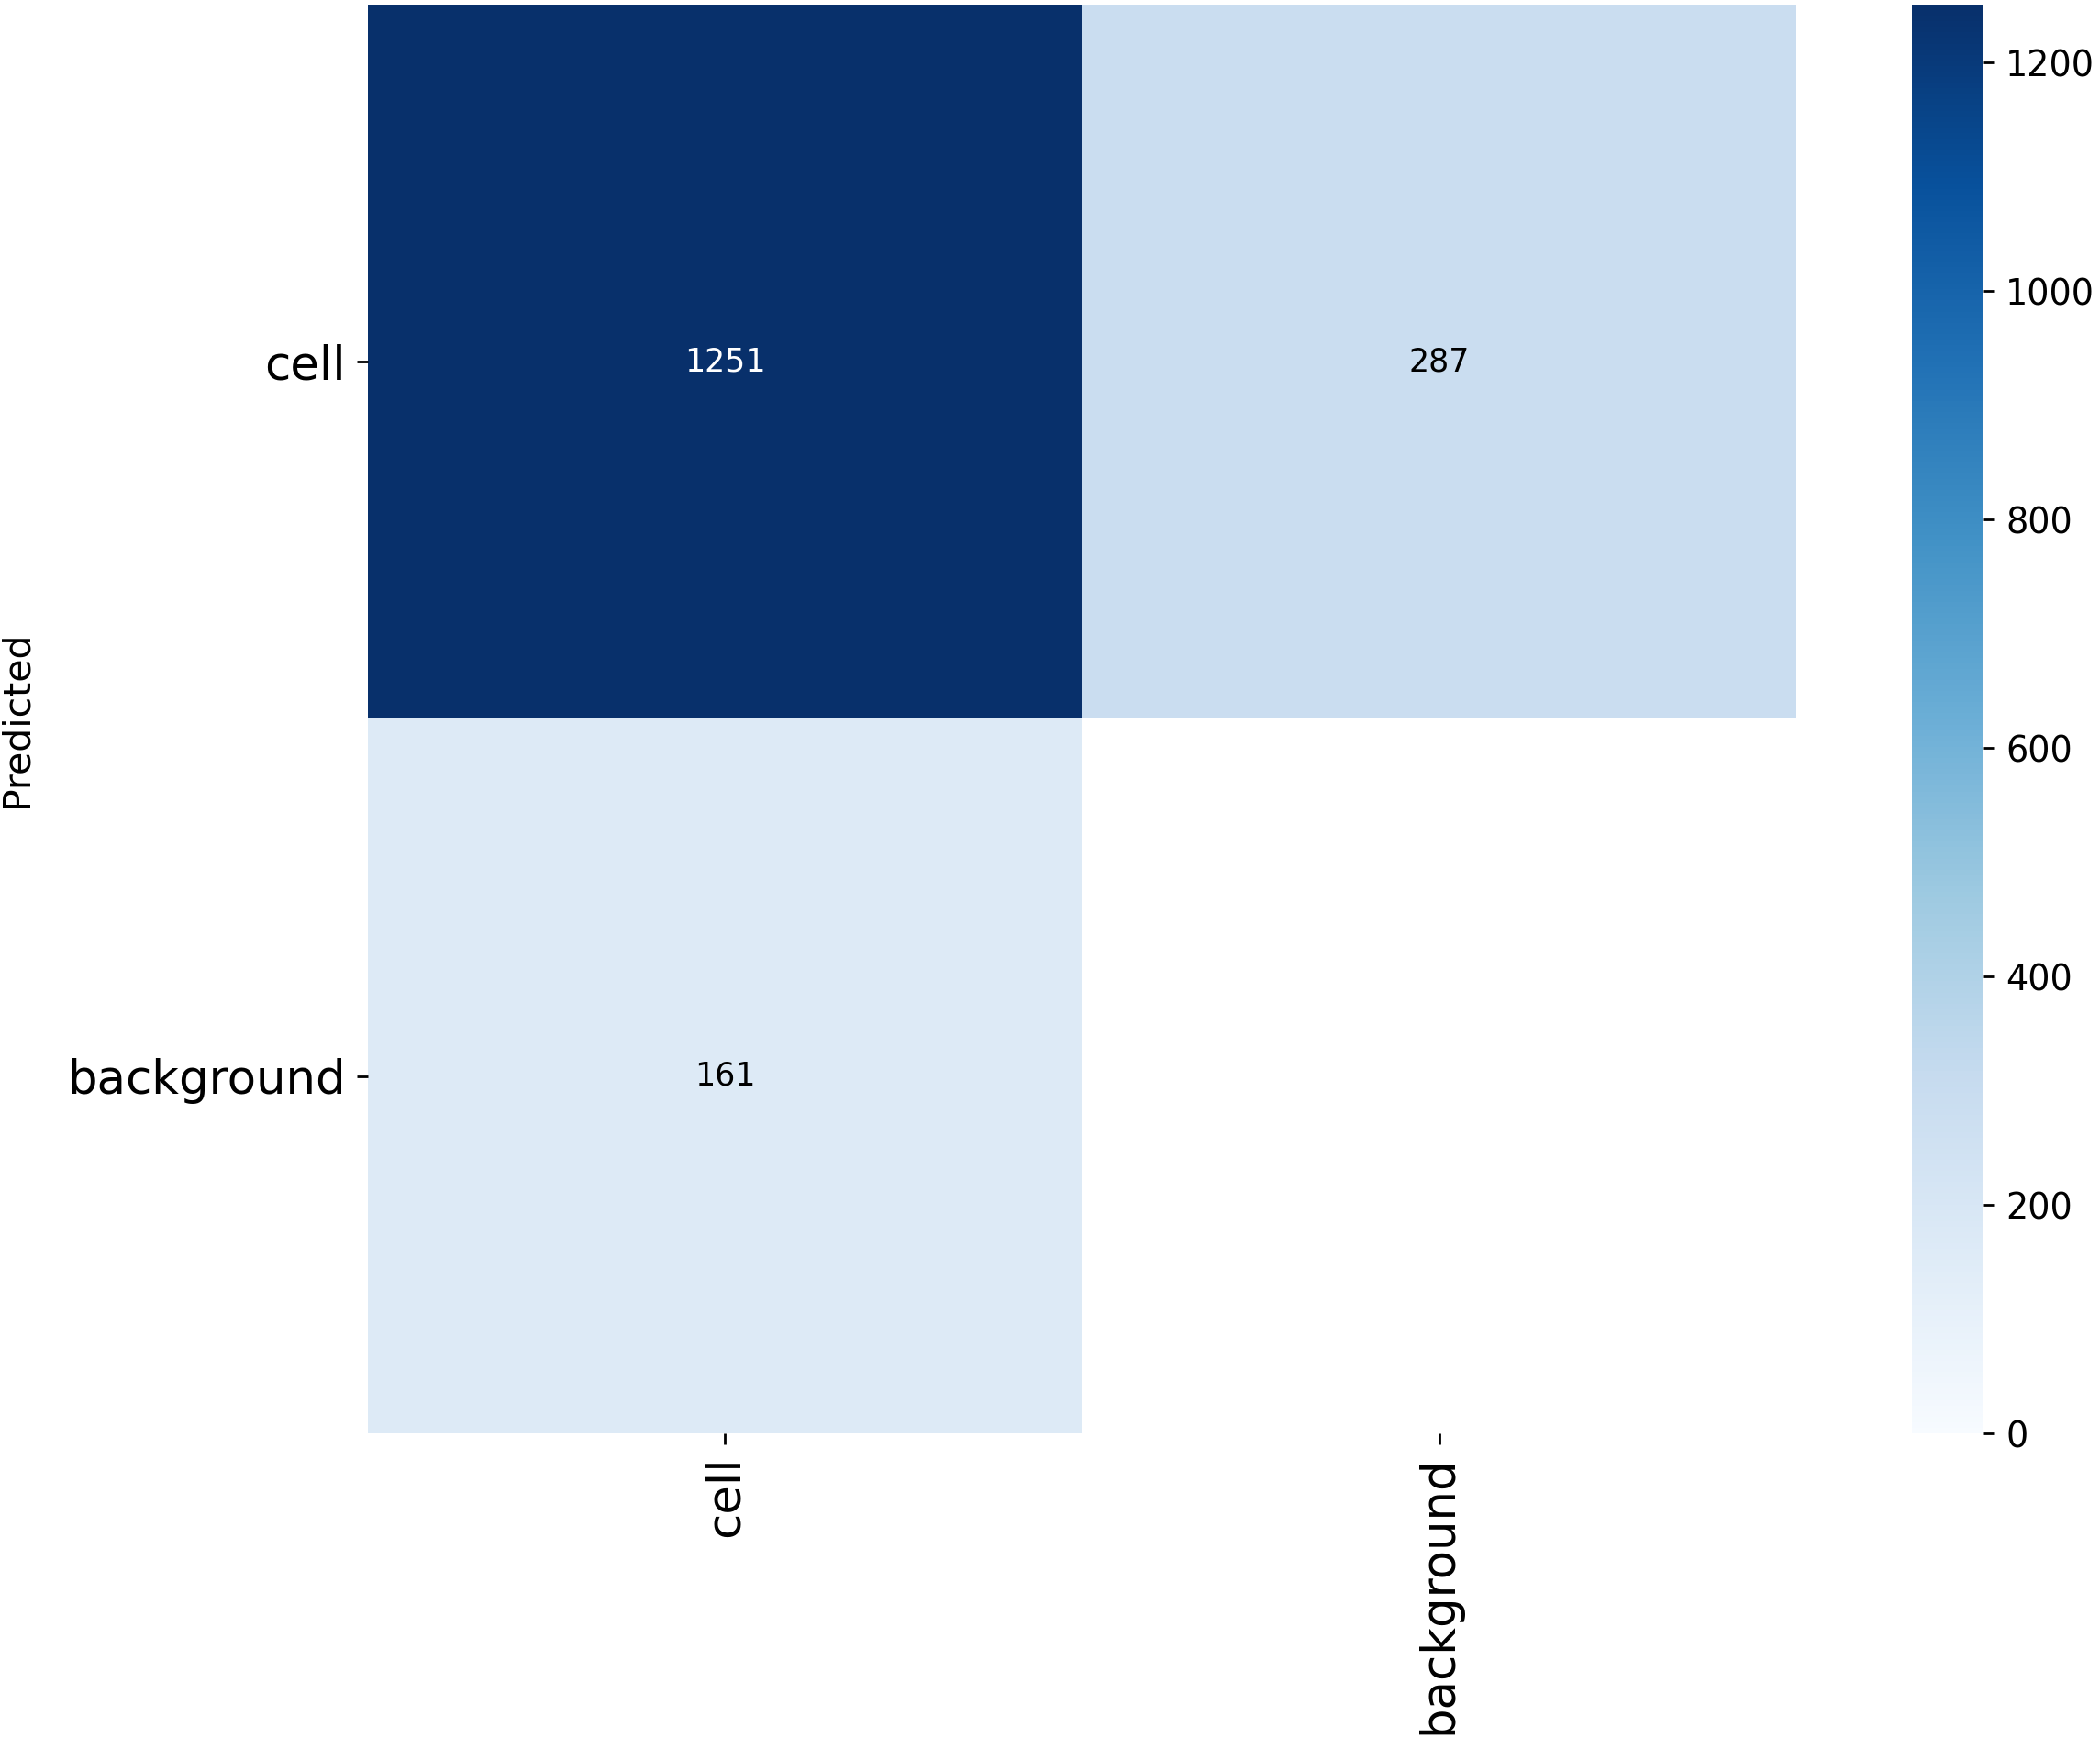
\includegraphics[height=5cm]{figuras/resultados experimentacion/custom/test/confusion_matrix.png}
    \vspace{-0.3cm}
    \caption{\footnotesize \textit{custom}}
    \label{fig:confusion_custom_test}
  \end{subfigure}
  \hfill
  \begin{subfigure}[b]{0.45\textwidth}
    \centering
    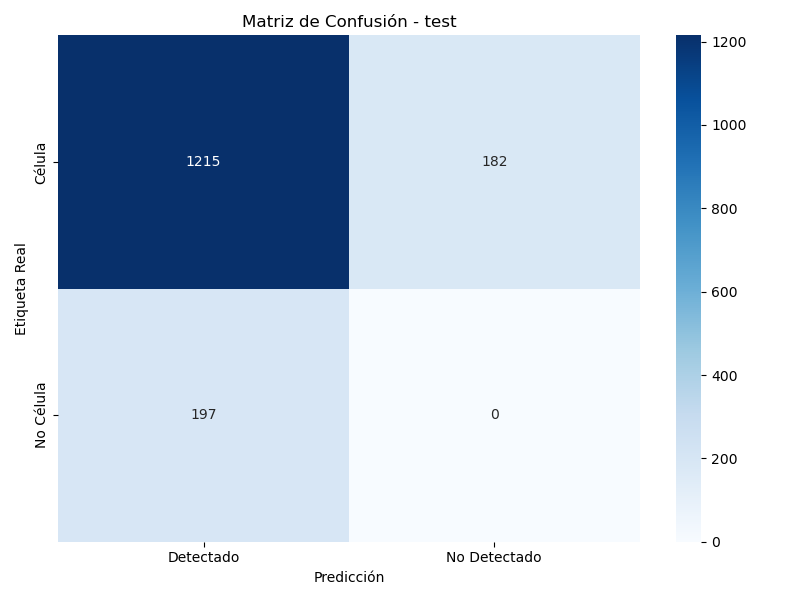
\includegraphics[height=5cm]{figuras/resultados experimentacion/ensemble/confusion_matrices/confusion_matrix_test.png}
    \vspace{-0.3cm}
    \caption{\footnotesize \textit{ensemble}}
    \label{fig:confusion_ensemble_test}
  \end{subfigure}
  
  \vspace{-0.2cm}
  \caption{Matrices de confusión para los modelos evaluados en test}
  \label{fig:confusion_matrices_test}
\end{figure}


% FIGURA PARA TEST2
\begin{figure}[H]
  \centering
  \vspace{-0.3cm}
  % Primera fila
  \begin{subfigure}[b]{0.45\textwidth}
    \centering
    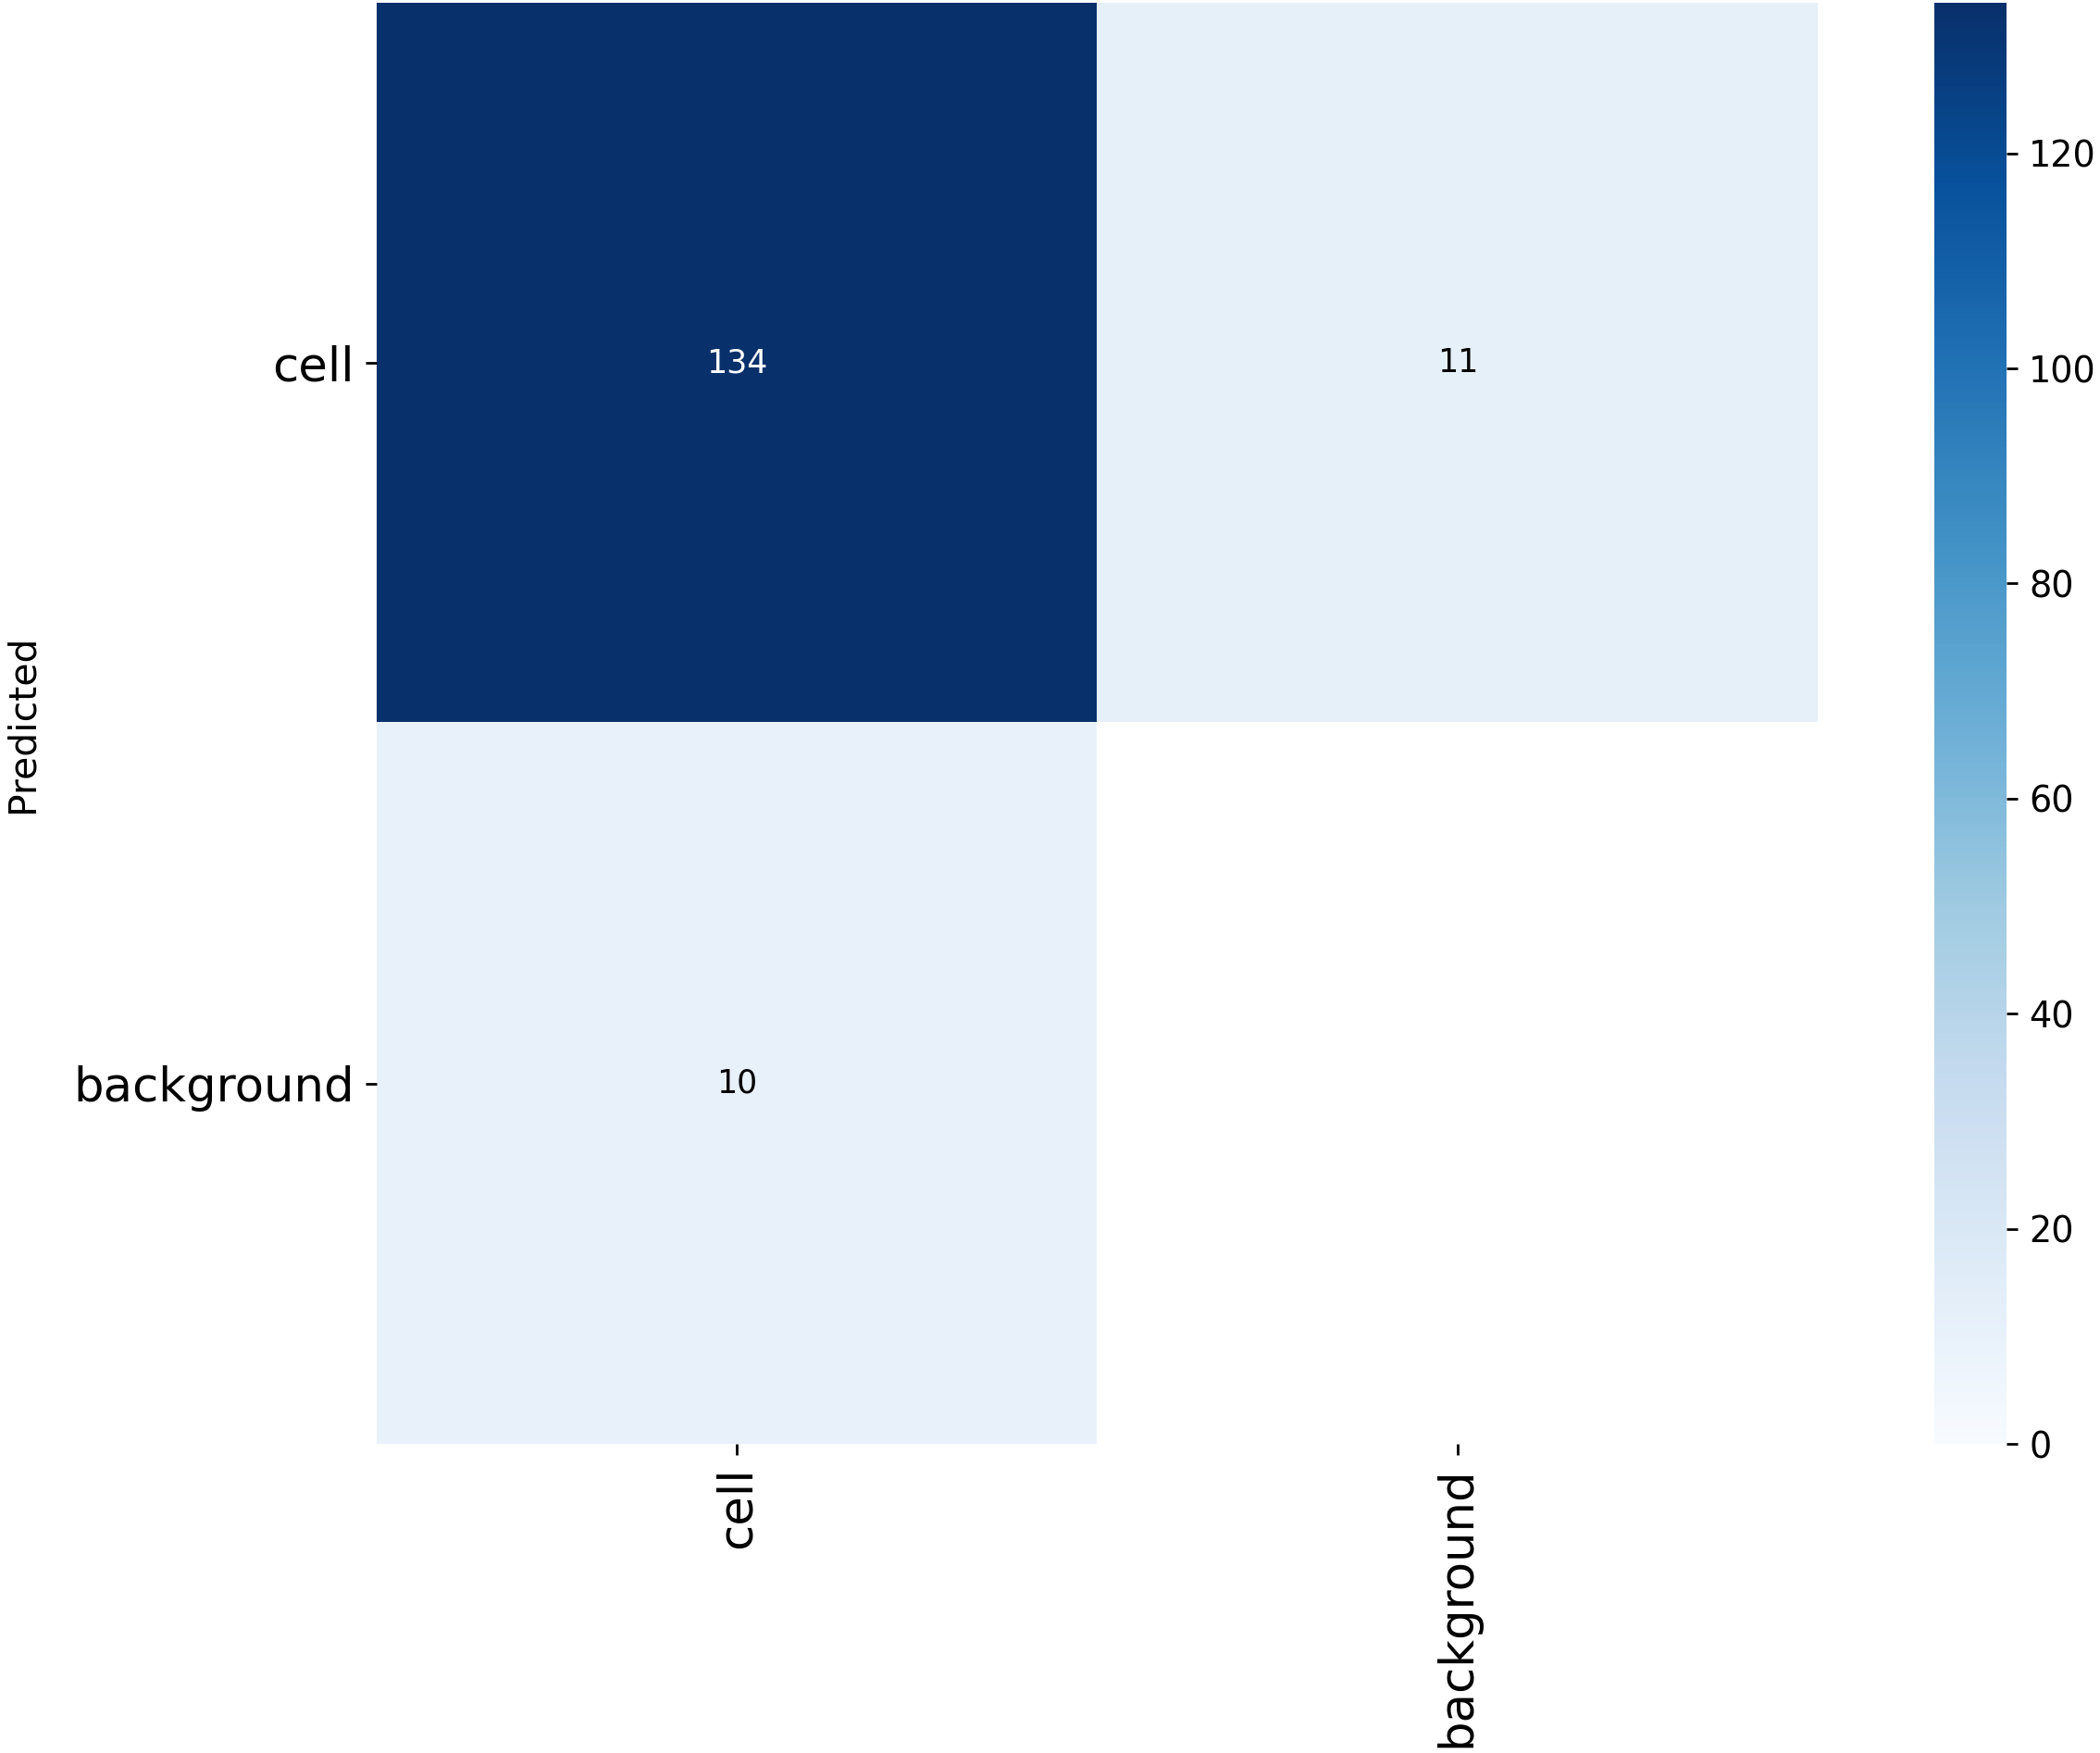
\includegraphics[height=5cm]{figuras/resultados experimentacion/yolov8s/test2/confusion_matrix.png}
    \vspace{-0.3cm}
    \caption{\footnotesize YOLOv8s}
    \label{fig:confusion_yolov8s_test2}
  \end{subfigure}
  \hfill
  \begin{subfigure}[b]{0.45\textwidth}
    \centering
    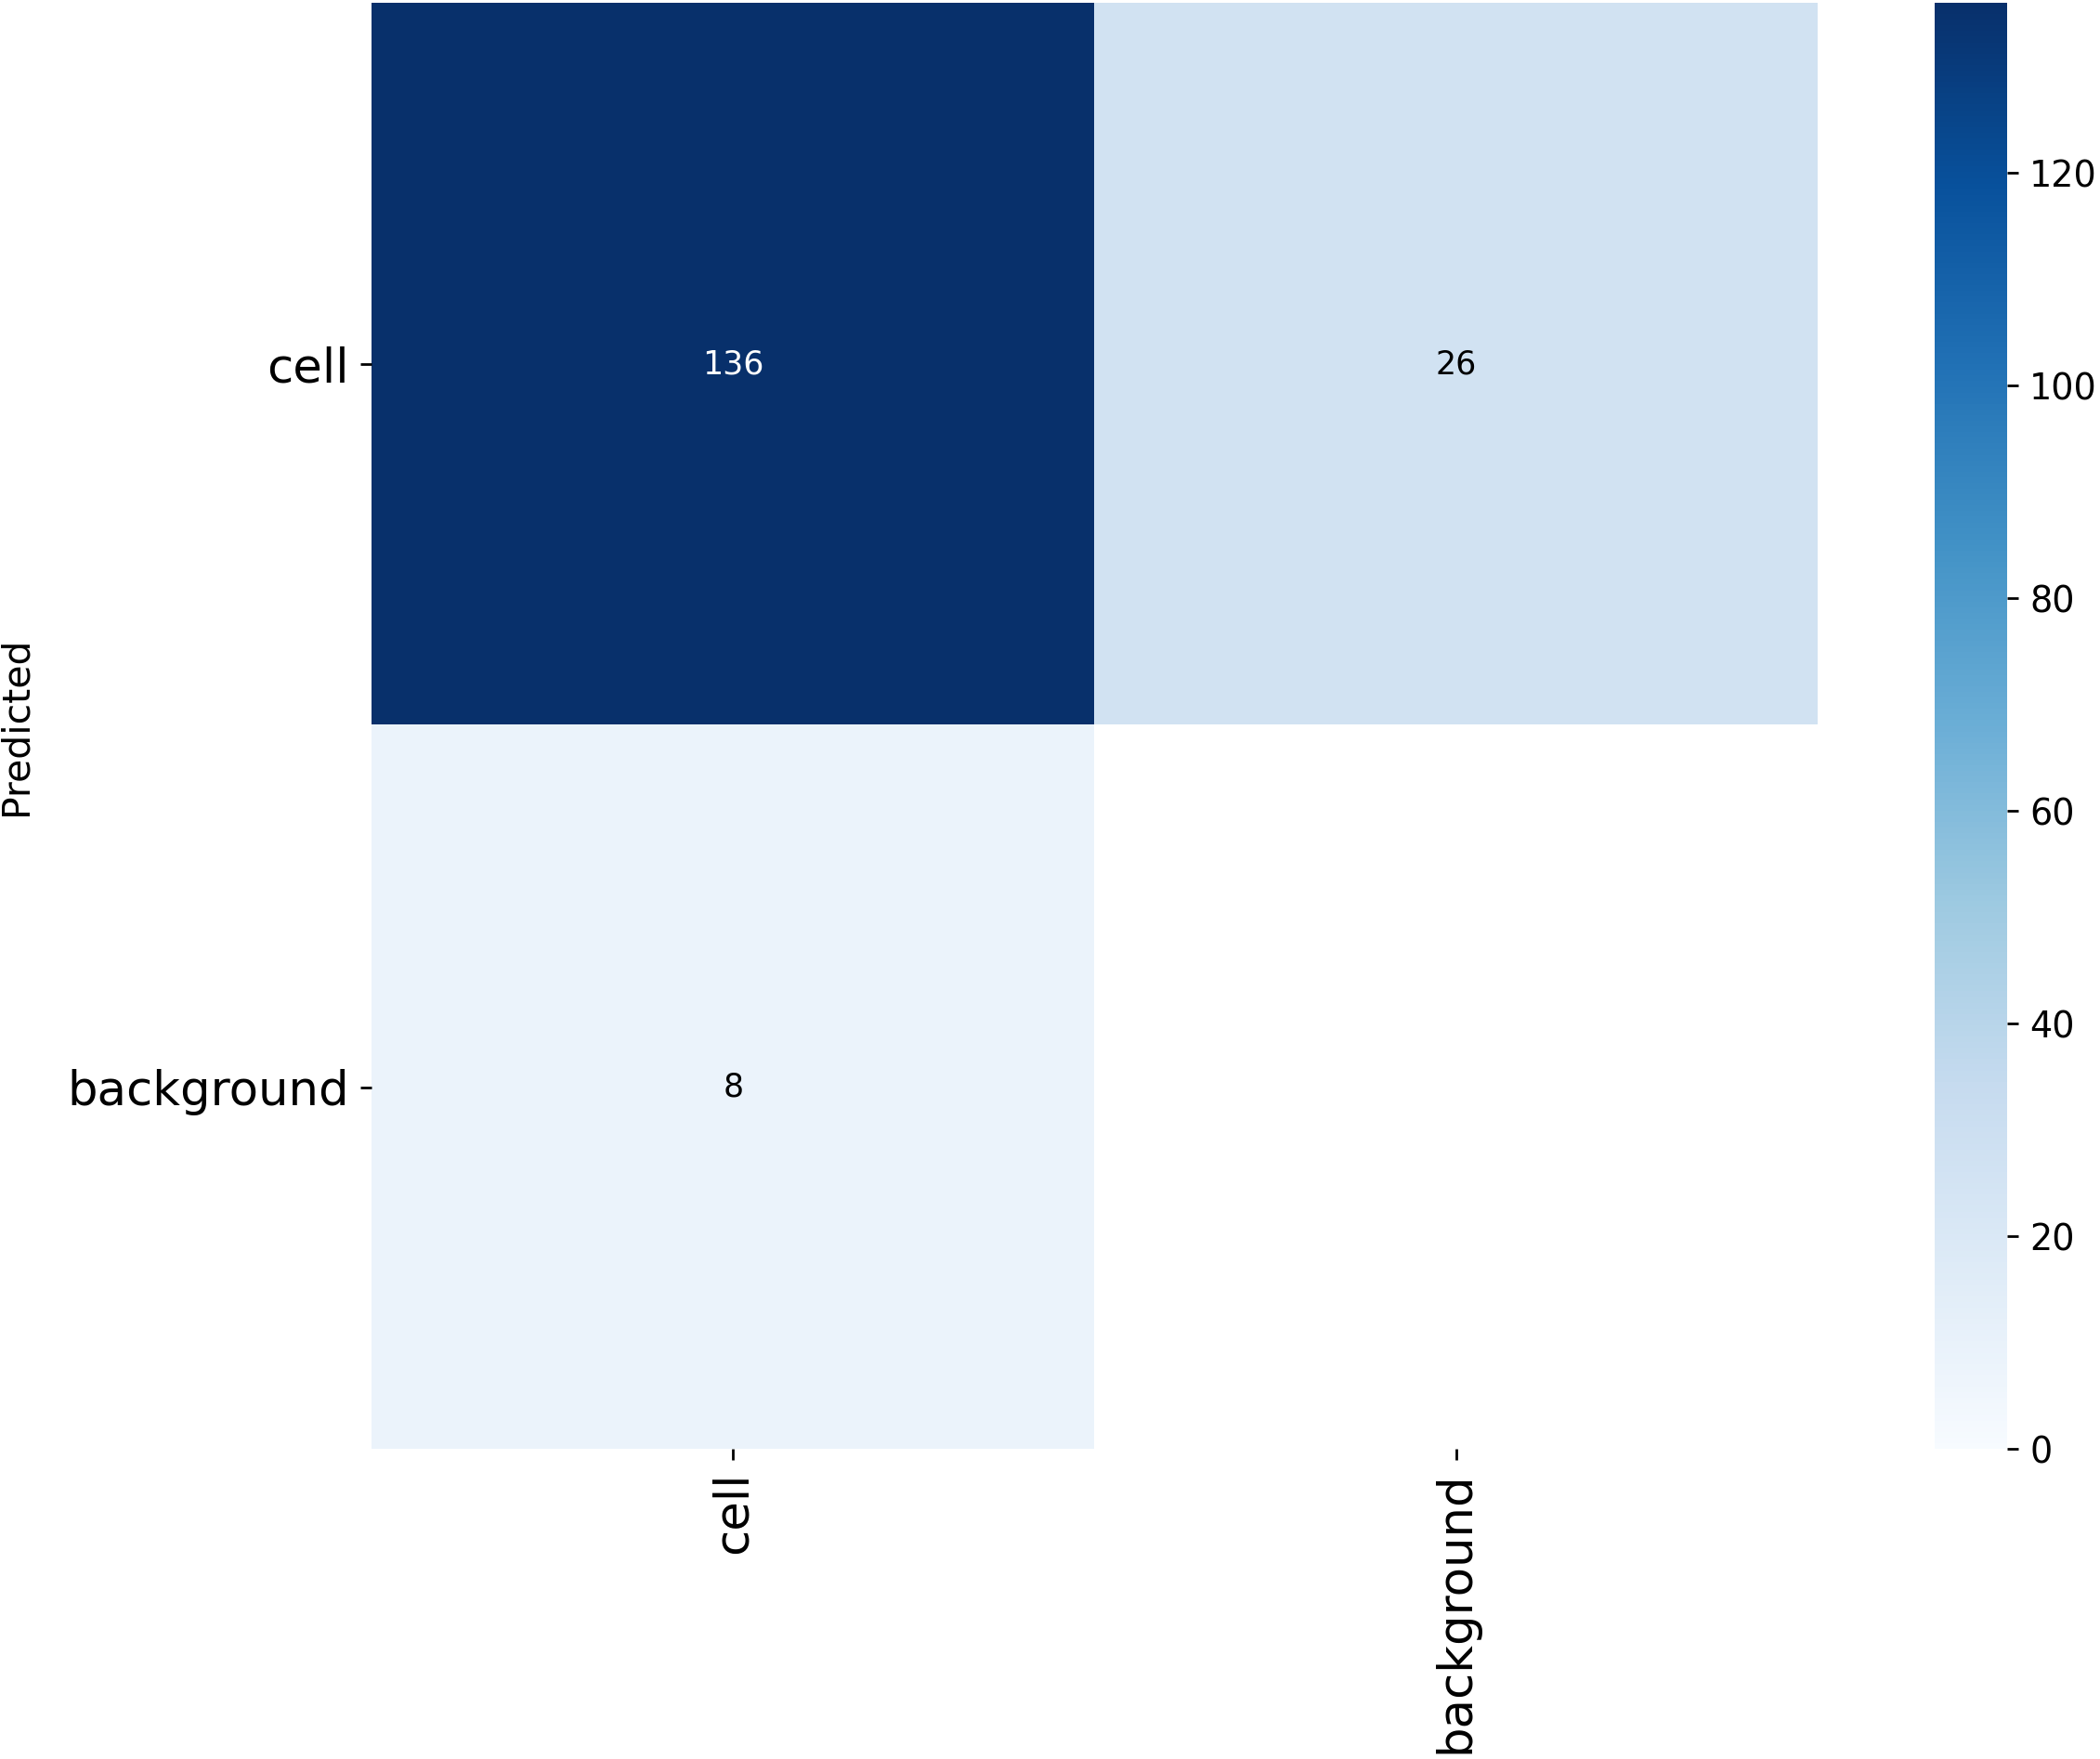
\includegraphics[height=5cm]{figuras/resultados experimentacion/yolov9s/test2/confusion_matrix.png}
    \vspace{-0.3cm}
    \caption{\footnotesize YOLOv9s}
    \label{fig:confusion_yolov9s_test2}
  \end{subfigure}
  
  \vspace{0.1cm}
  % Segunda fila
  \begin{subfigure}[b]{0.45\textwidth}
    \centering
    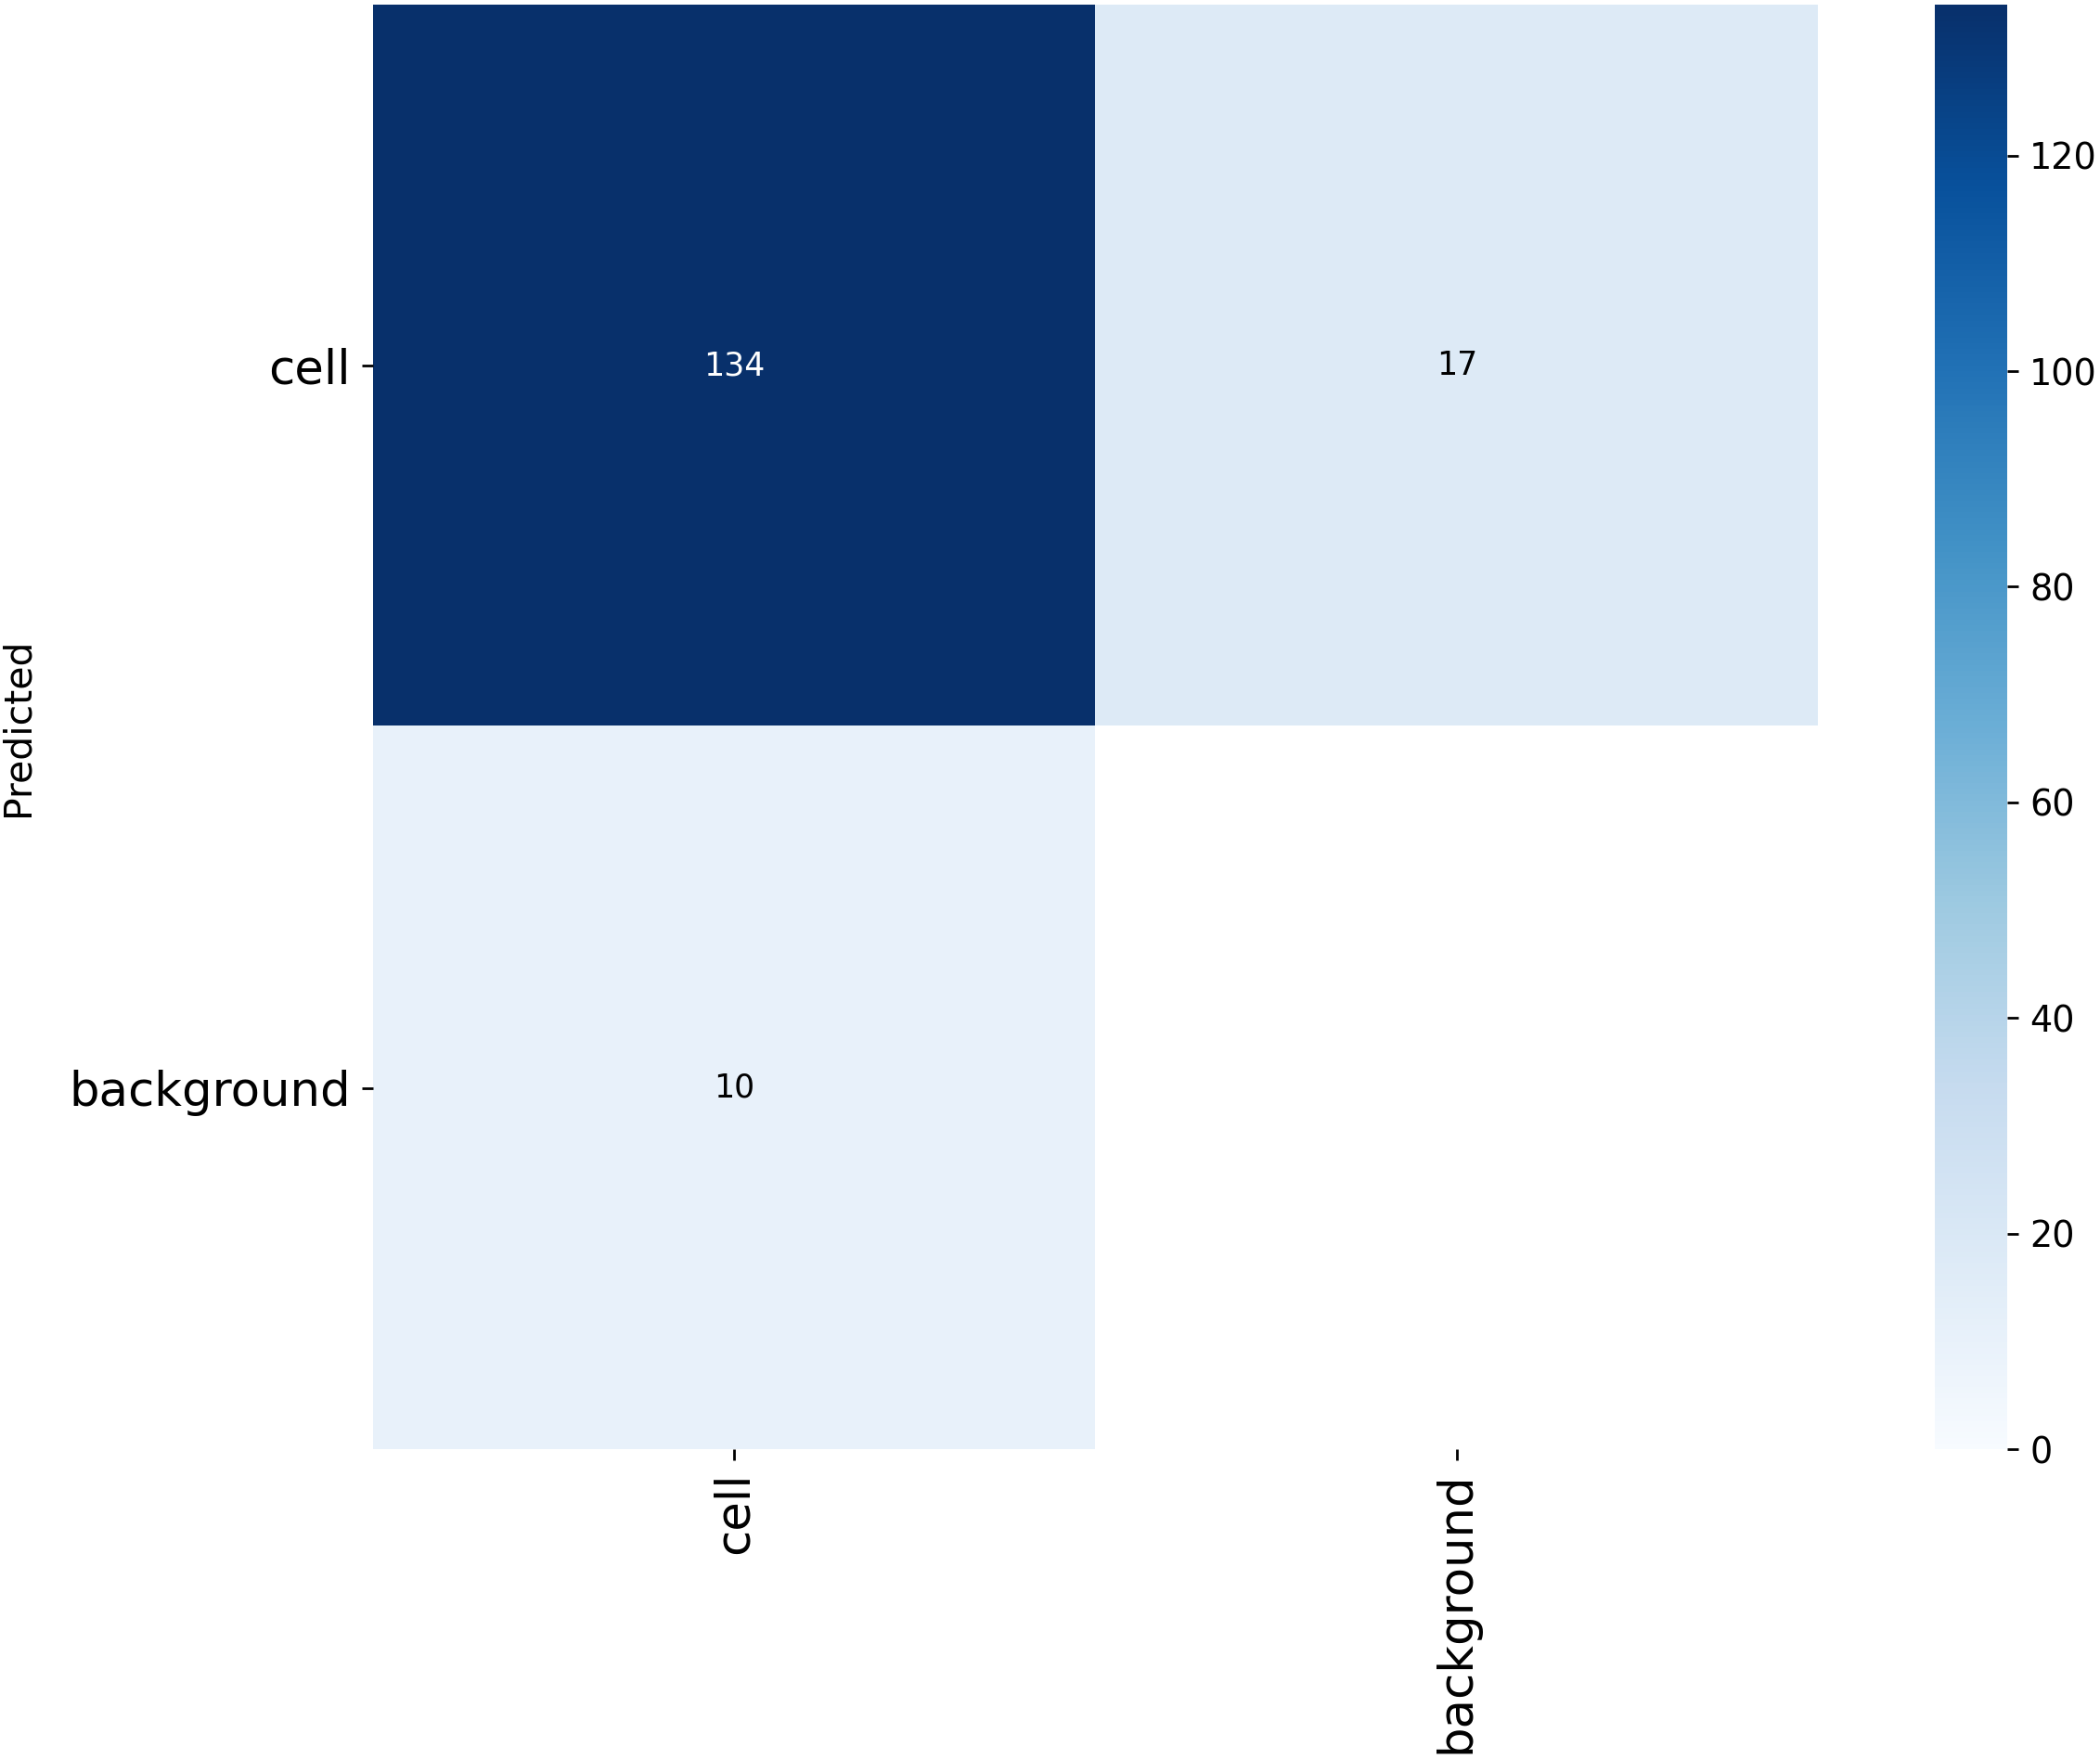
\includegraphics[height=5cm]{figuras/resultados experimentacion/yolov10s/test2/confusion_matrix.png}
    \vspace{-0.3cm}
    \caption{\footnotesize YOLOv10s}
    \label{fig:confusion_yolov10s_test2}
  \end{subfigure}
  \hfill
  \begin{subfigure}[b]{0.45\textwidth}
    \centering
    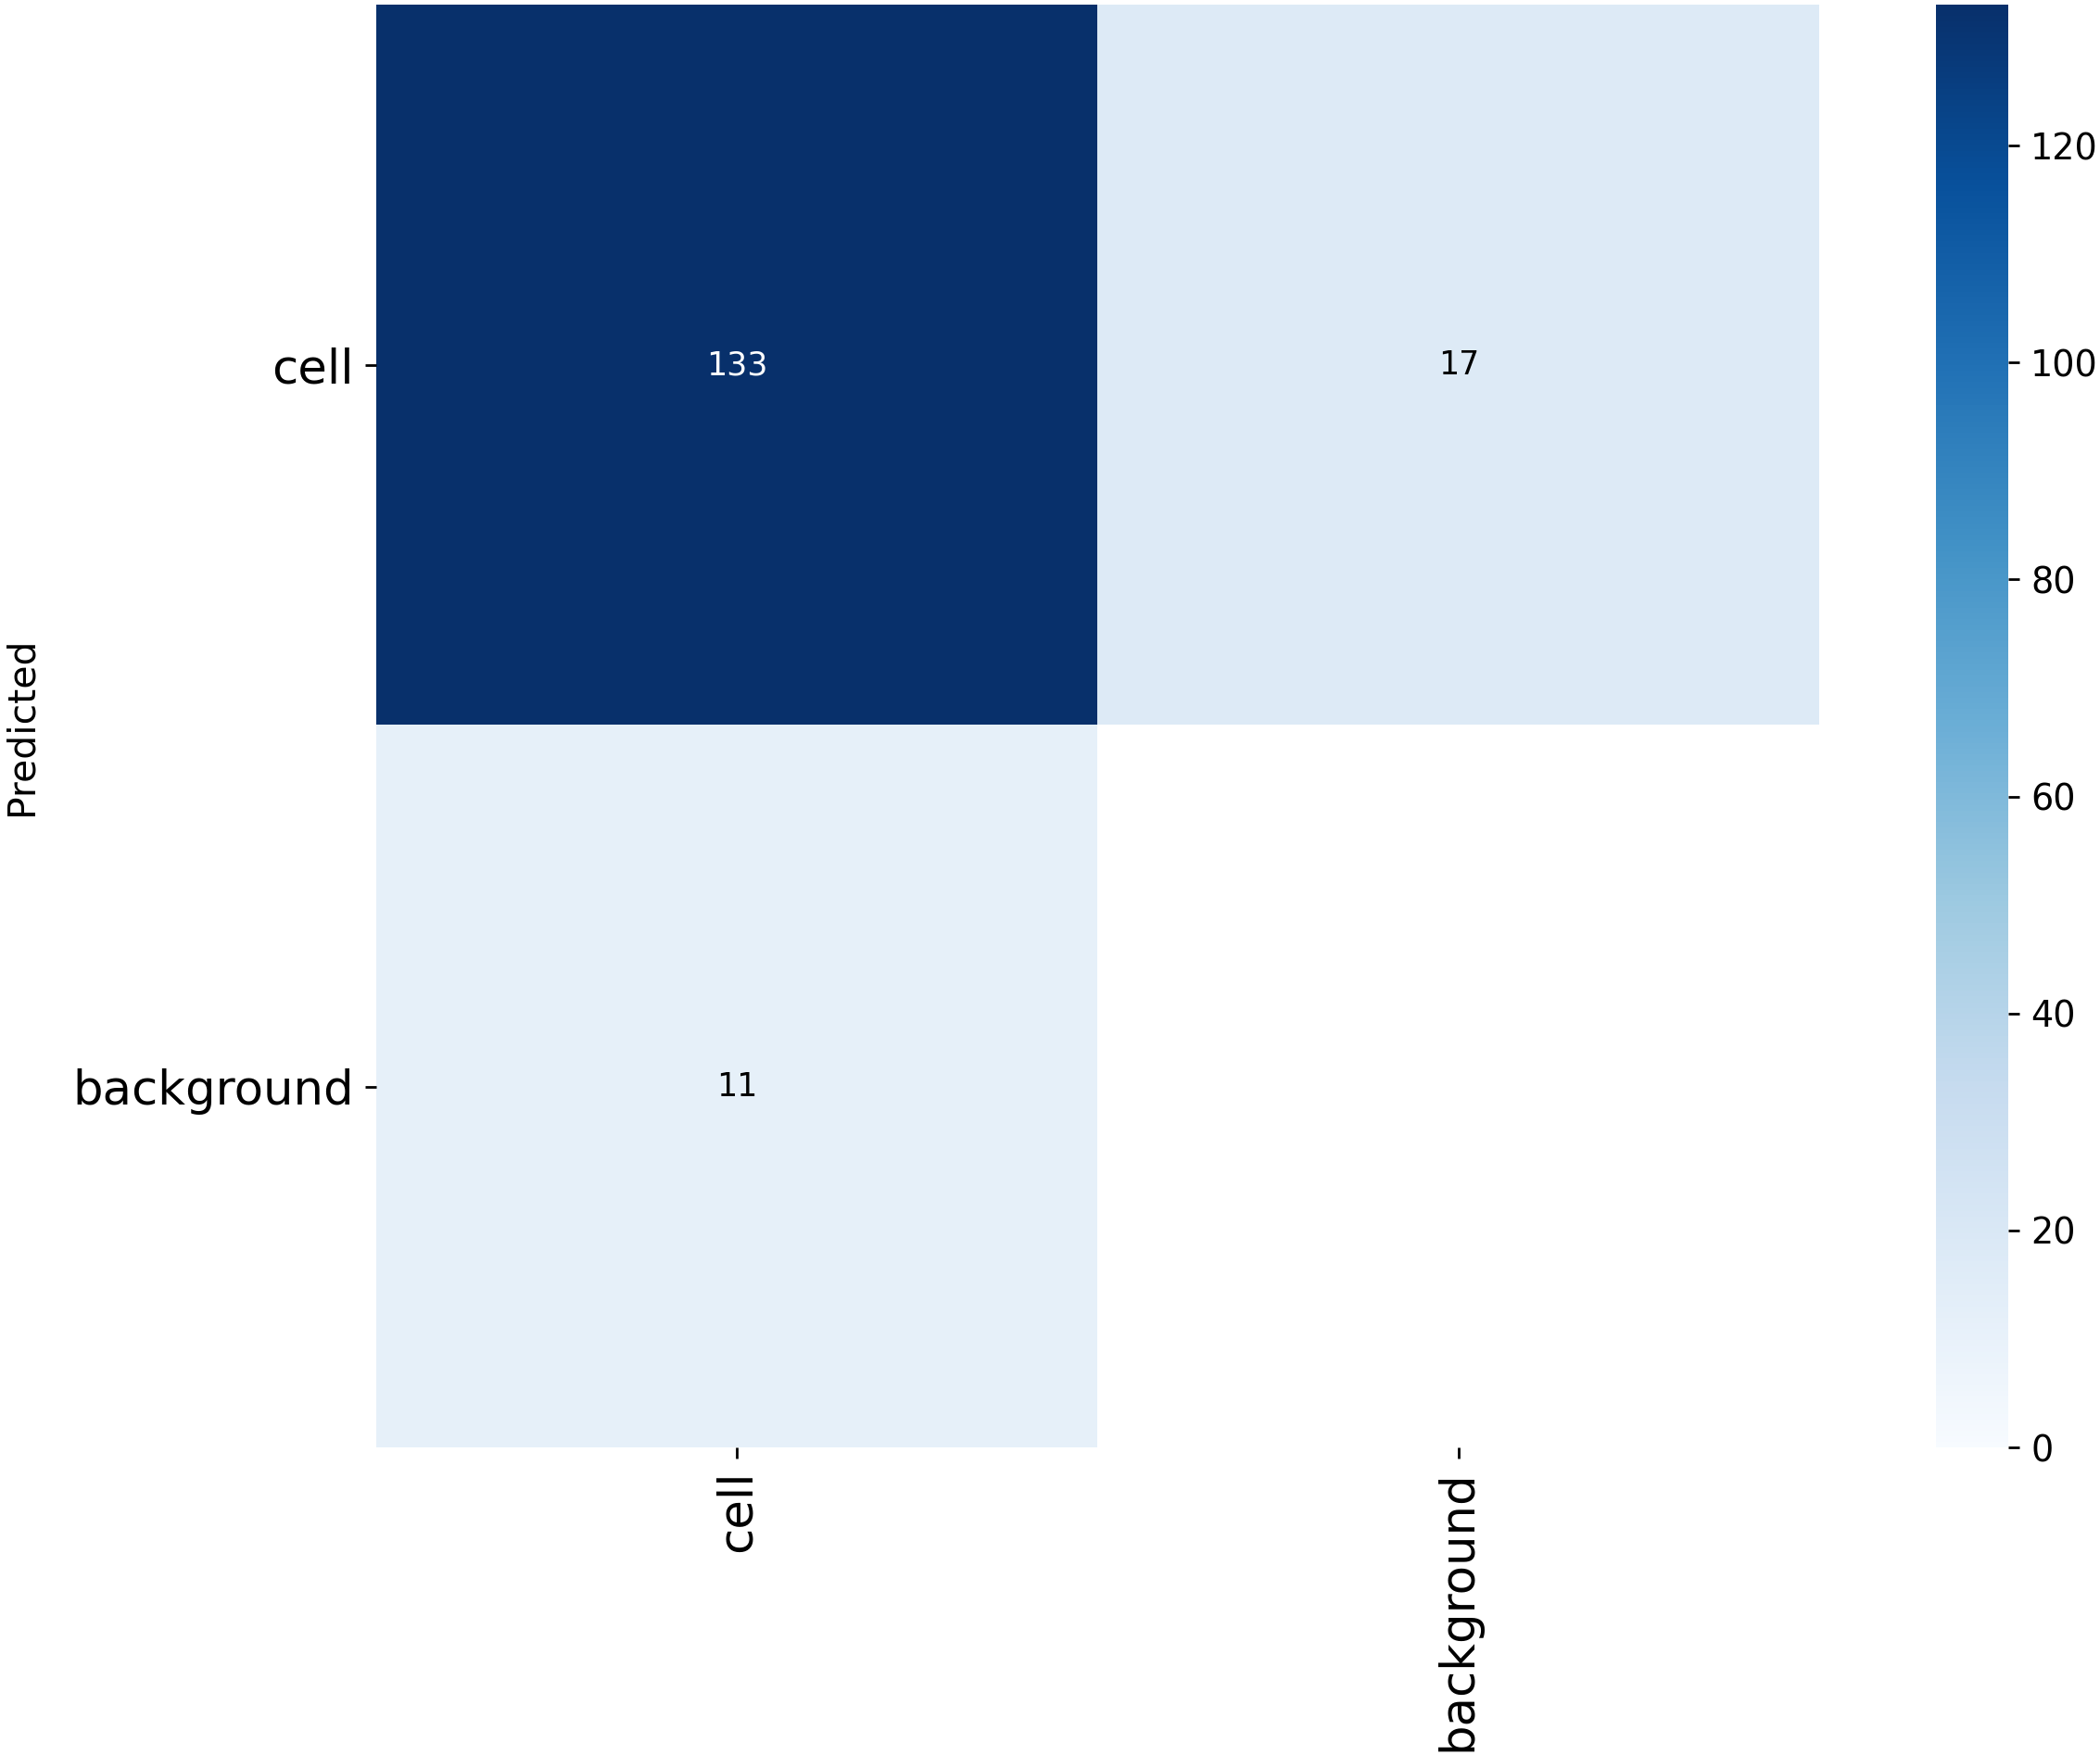
\includegraphics[height=5cm]{figuras/resultados experimentacion/yolov11s/test2/confusion_matrix.png}
    \vspace{-0.3cm}
    \caption{\footnotesize YOLOv11s}
    \label{fig:confusion_yolov11s_test2}
  \end{subfigure}
  
  \vspace{0.1cm}
  % Tercera fila
  \begin{subfigure}[b]{0.45\textwidth}
    \centering
    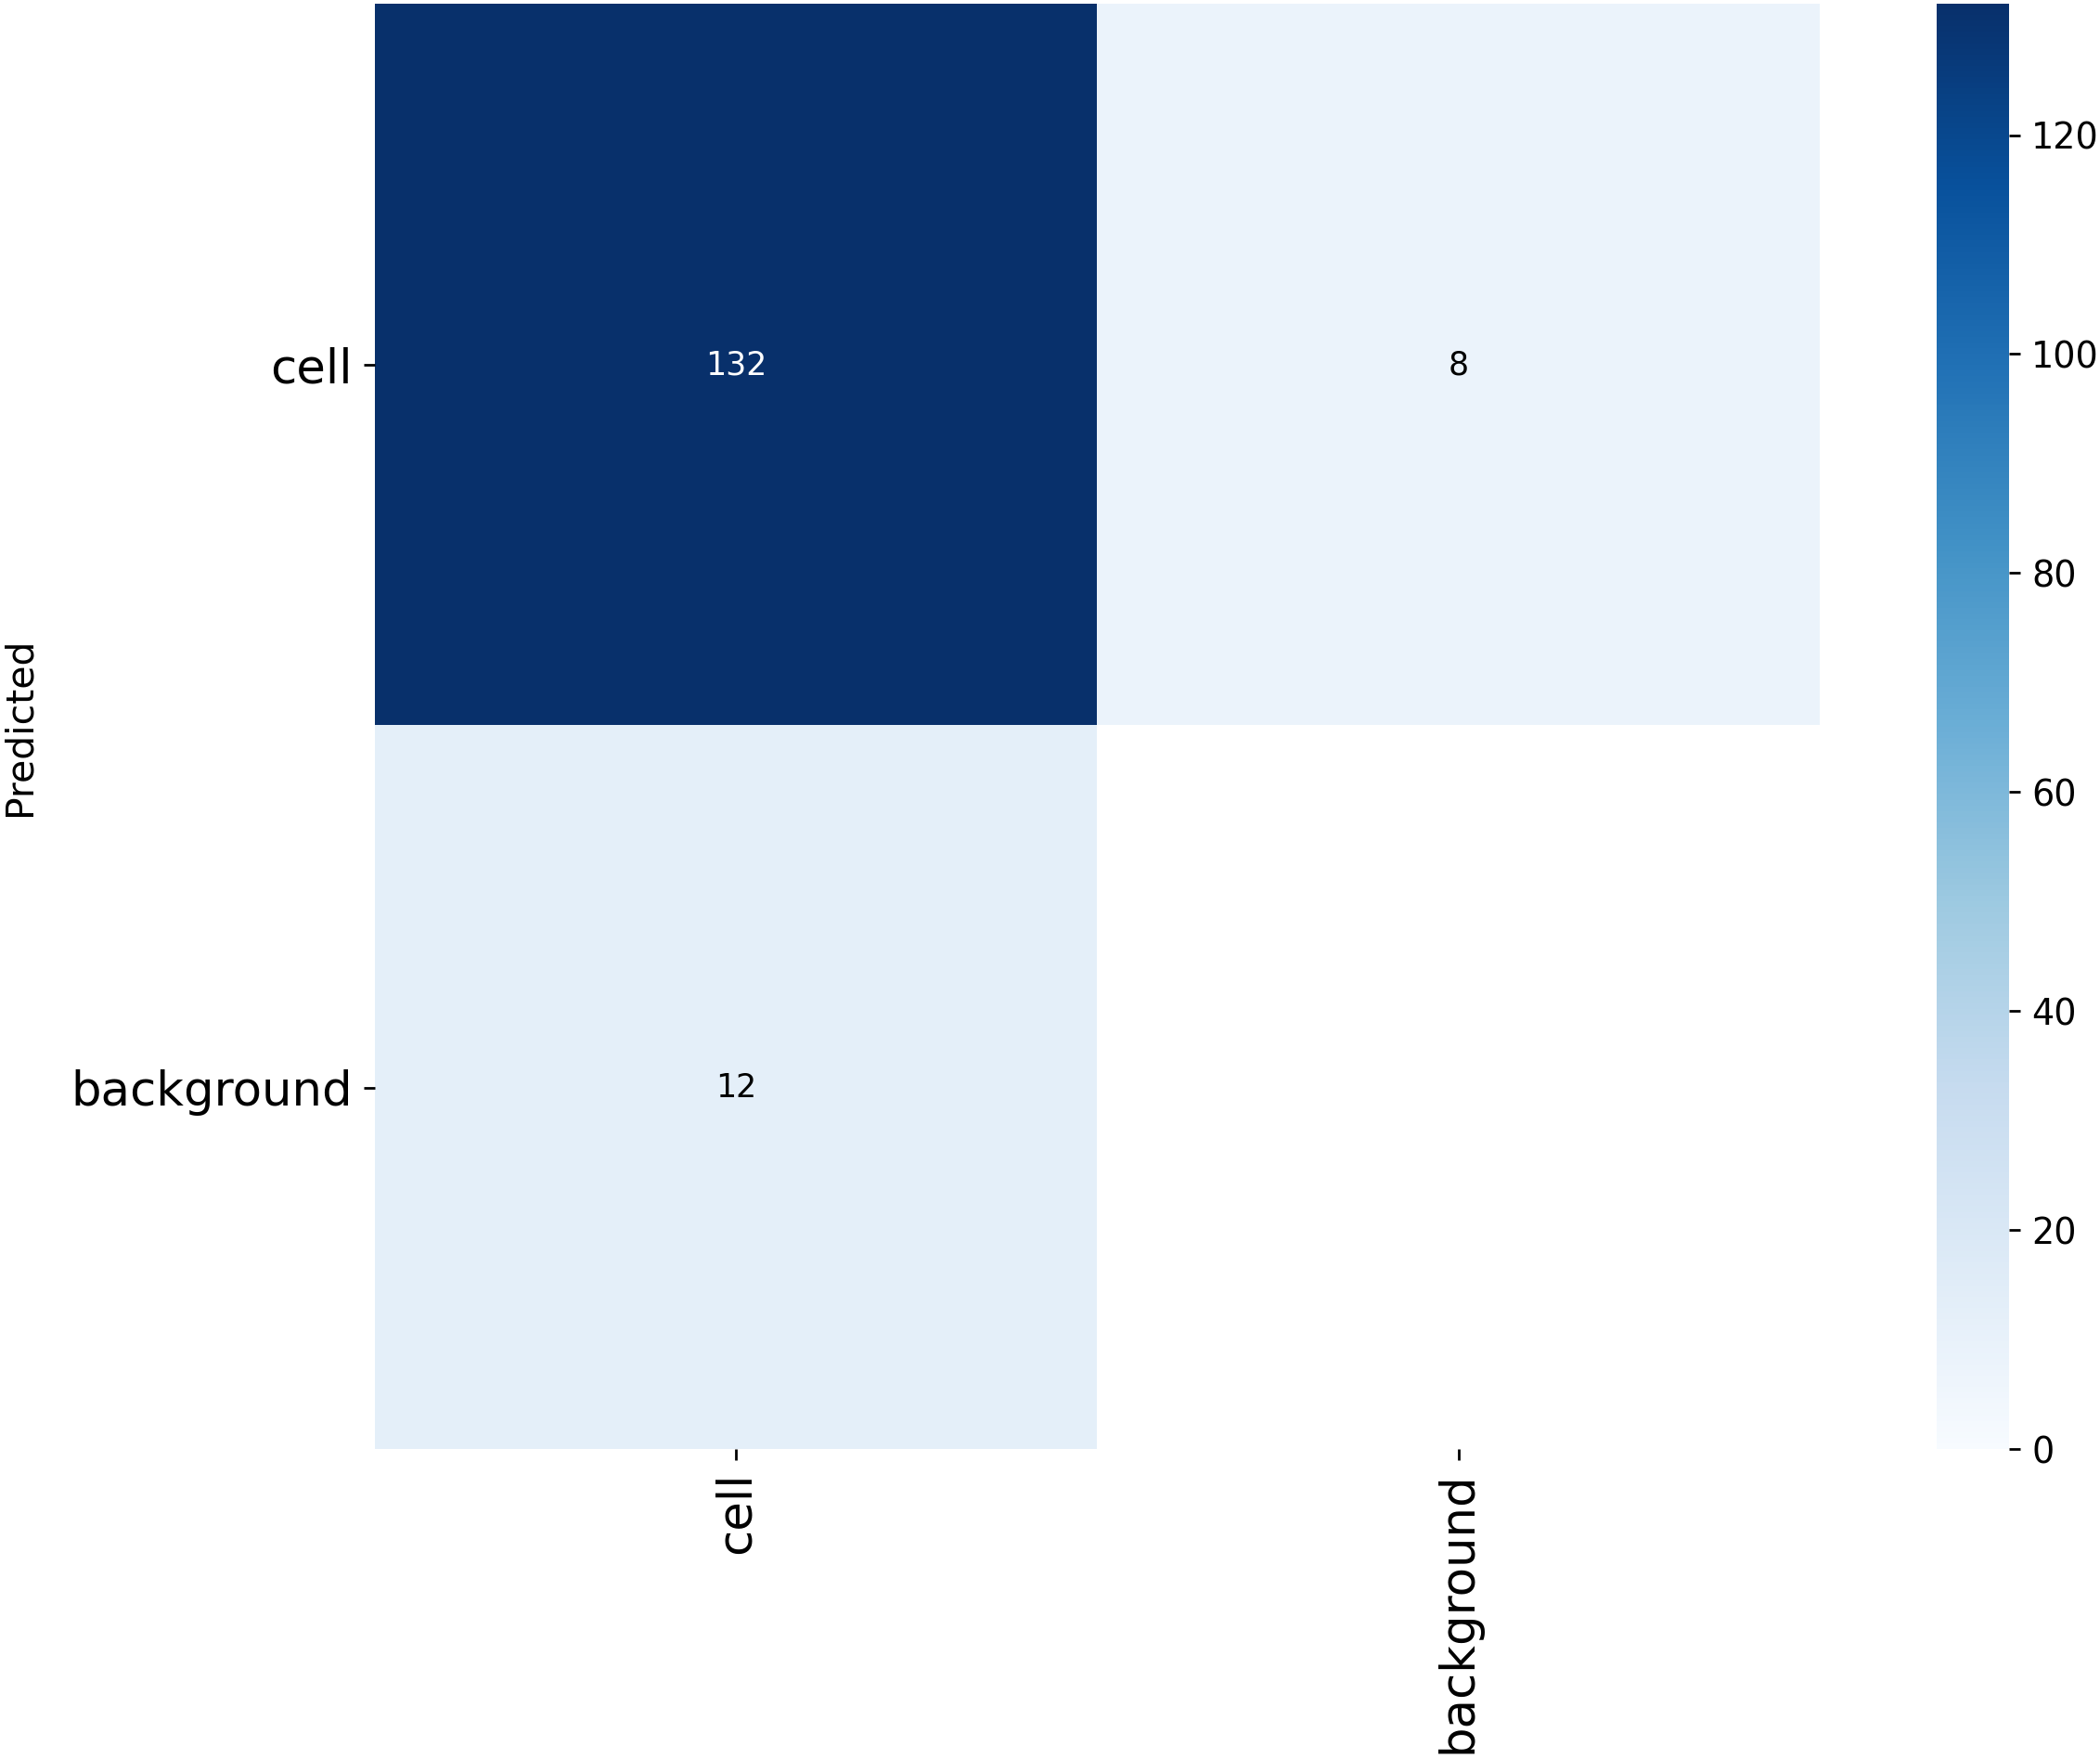
\includegraphics[height=5cm]{figuras/resultados experimentacion/yolov12s/test2/confusion_matrix.png}
    \vspace{-0.3cm}
    \caption{\footnotesize YOLOv12s}
    \label{fig:confusion_yolov12s_test2}
  \end{subfigure}
  \hfill
  \begin{subfigure}[b]{0.45\textwidth}
    \centering
    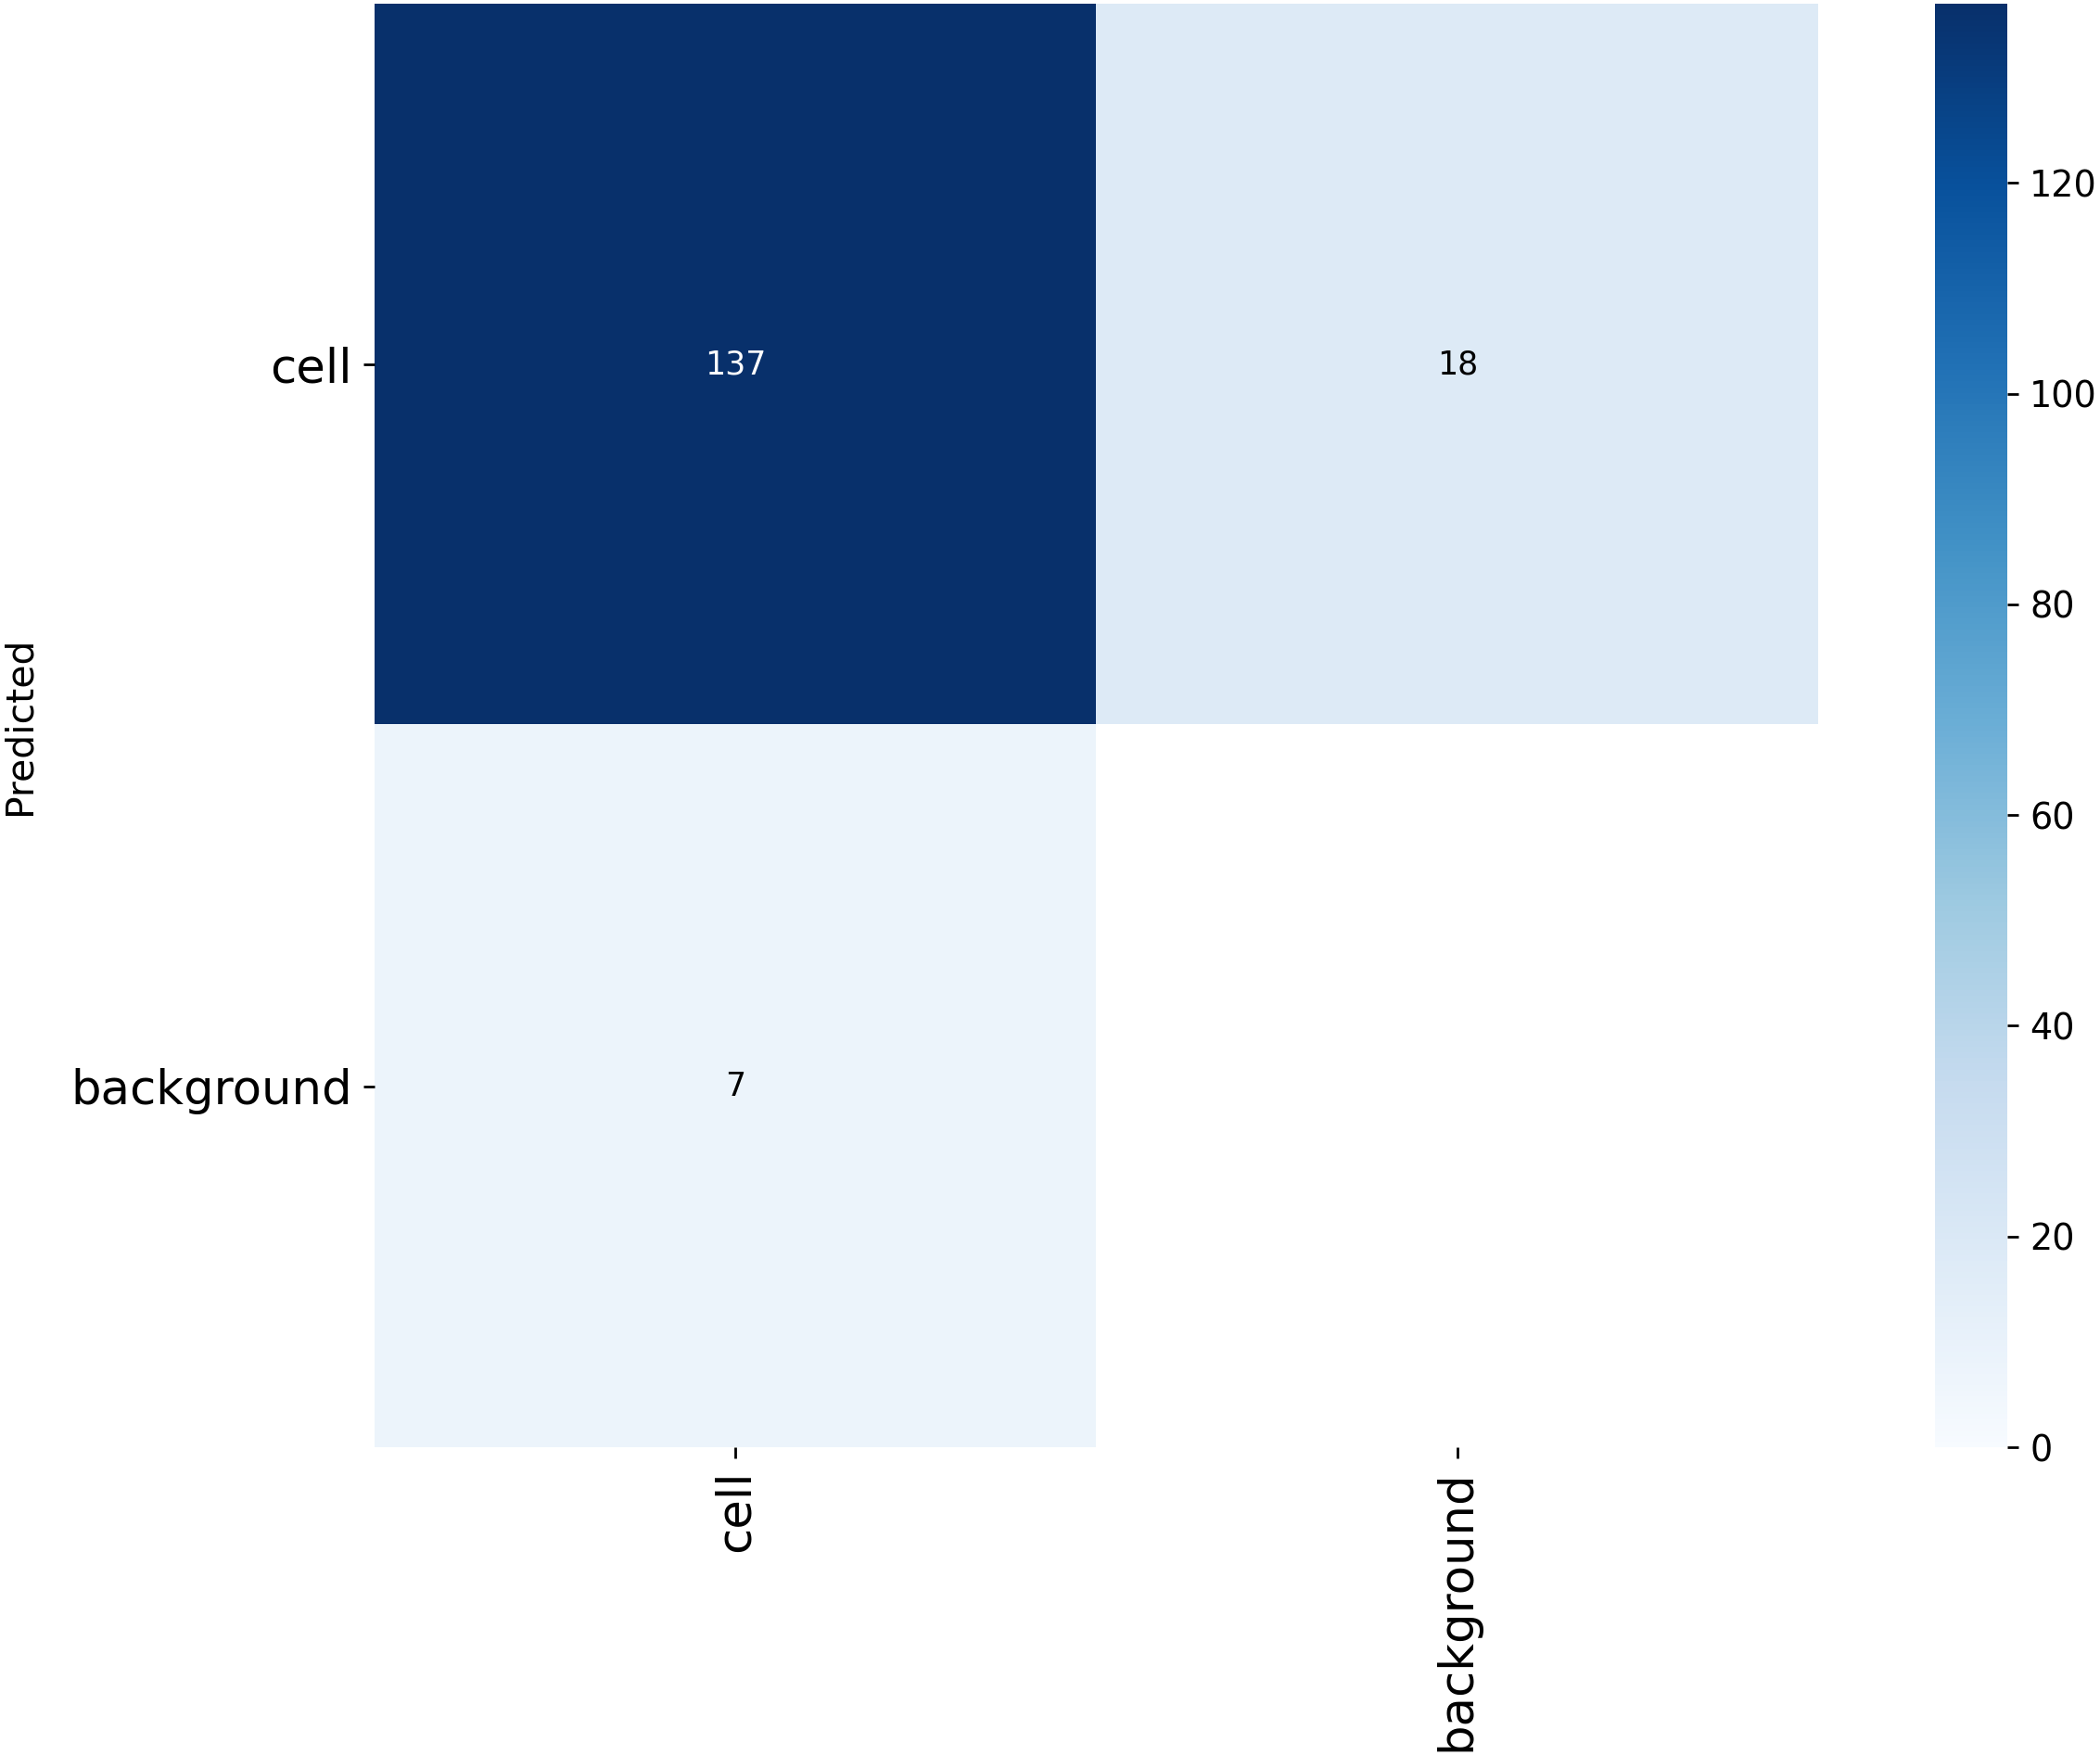
\includegraphics[height=5cm]{figuras/resultados experimentacion/yolov12l/test2/confusion_matrix.png}
    \vspace{-0.3cm}
    \caption{\footnotesize YOLOv12l}
    \label{fig:confusion_yolov12l_test2}
  \end{subfigure}
  
  \vspace{0.1cm}
  % Cuarta fila
  \begin{subfigure}[b]{0.45\textwidth}
    \centering
    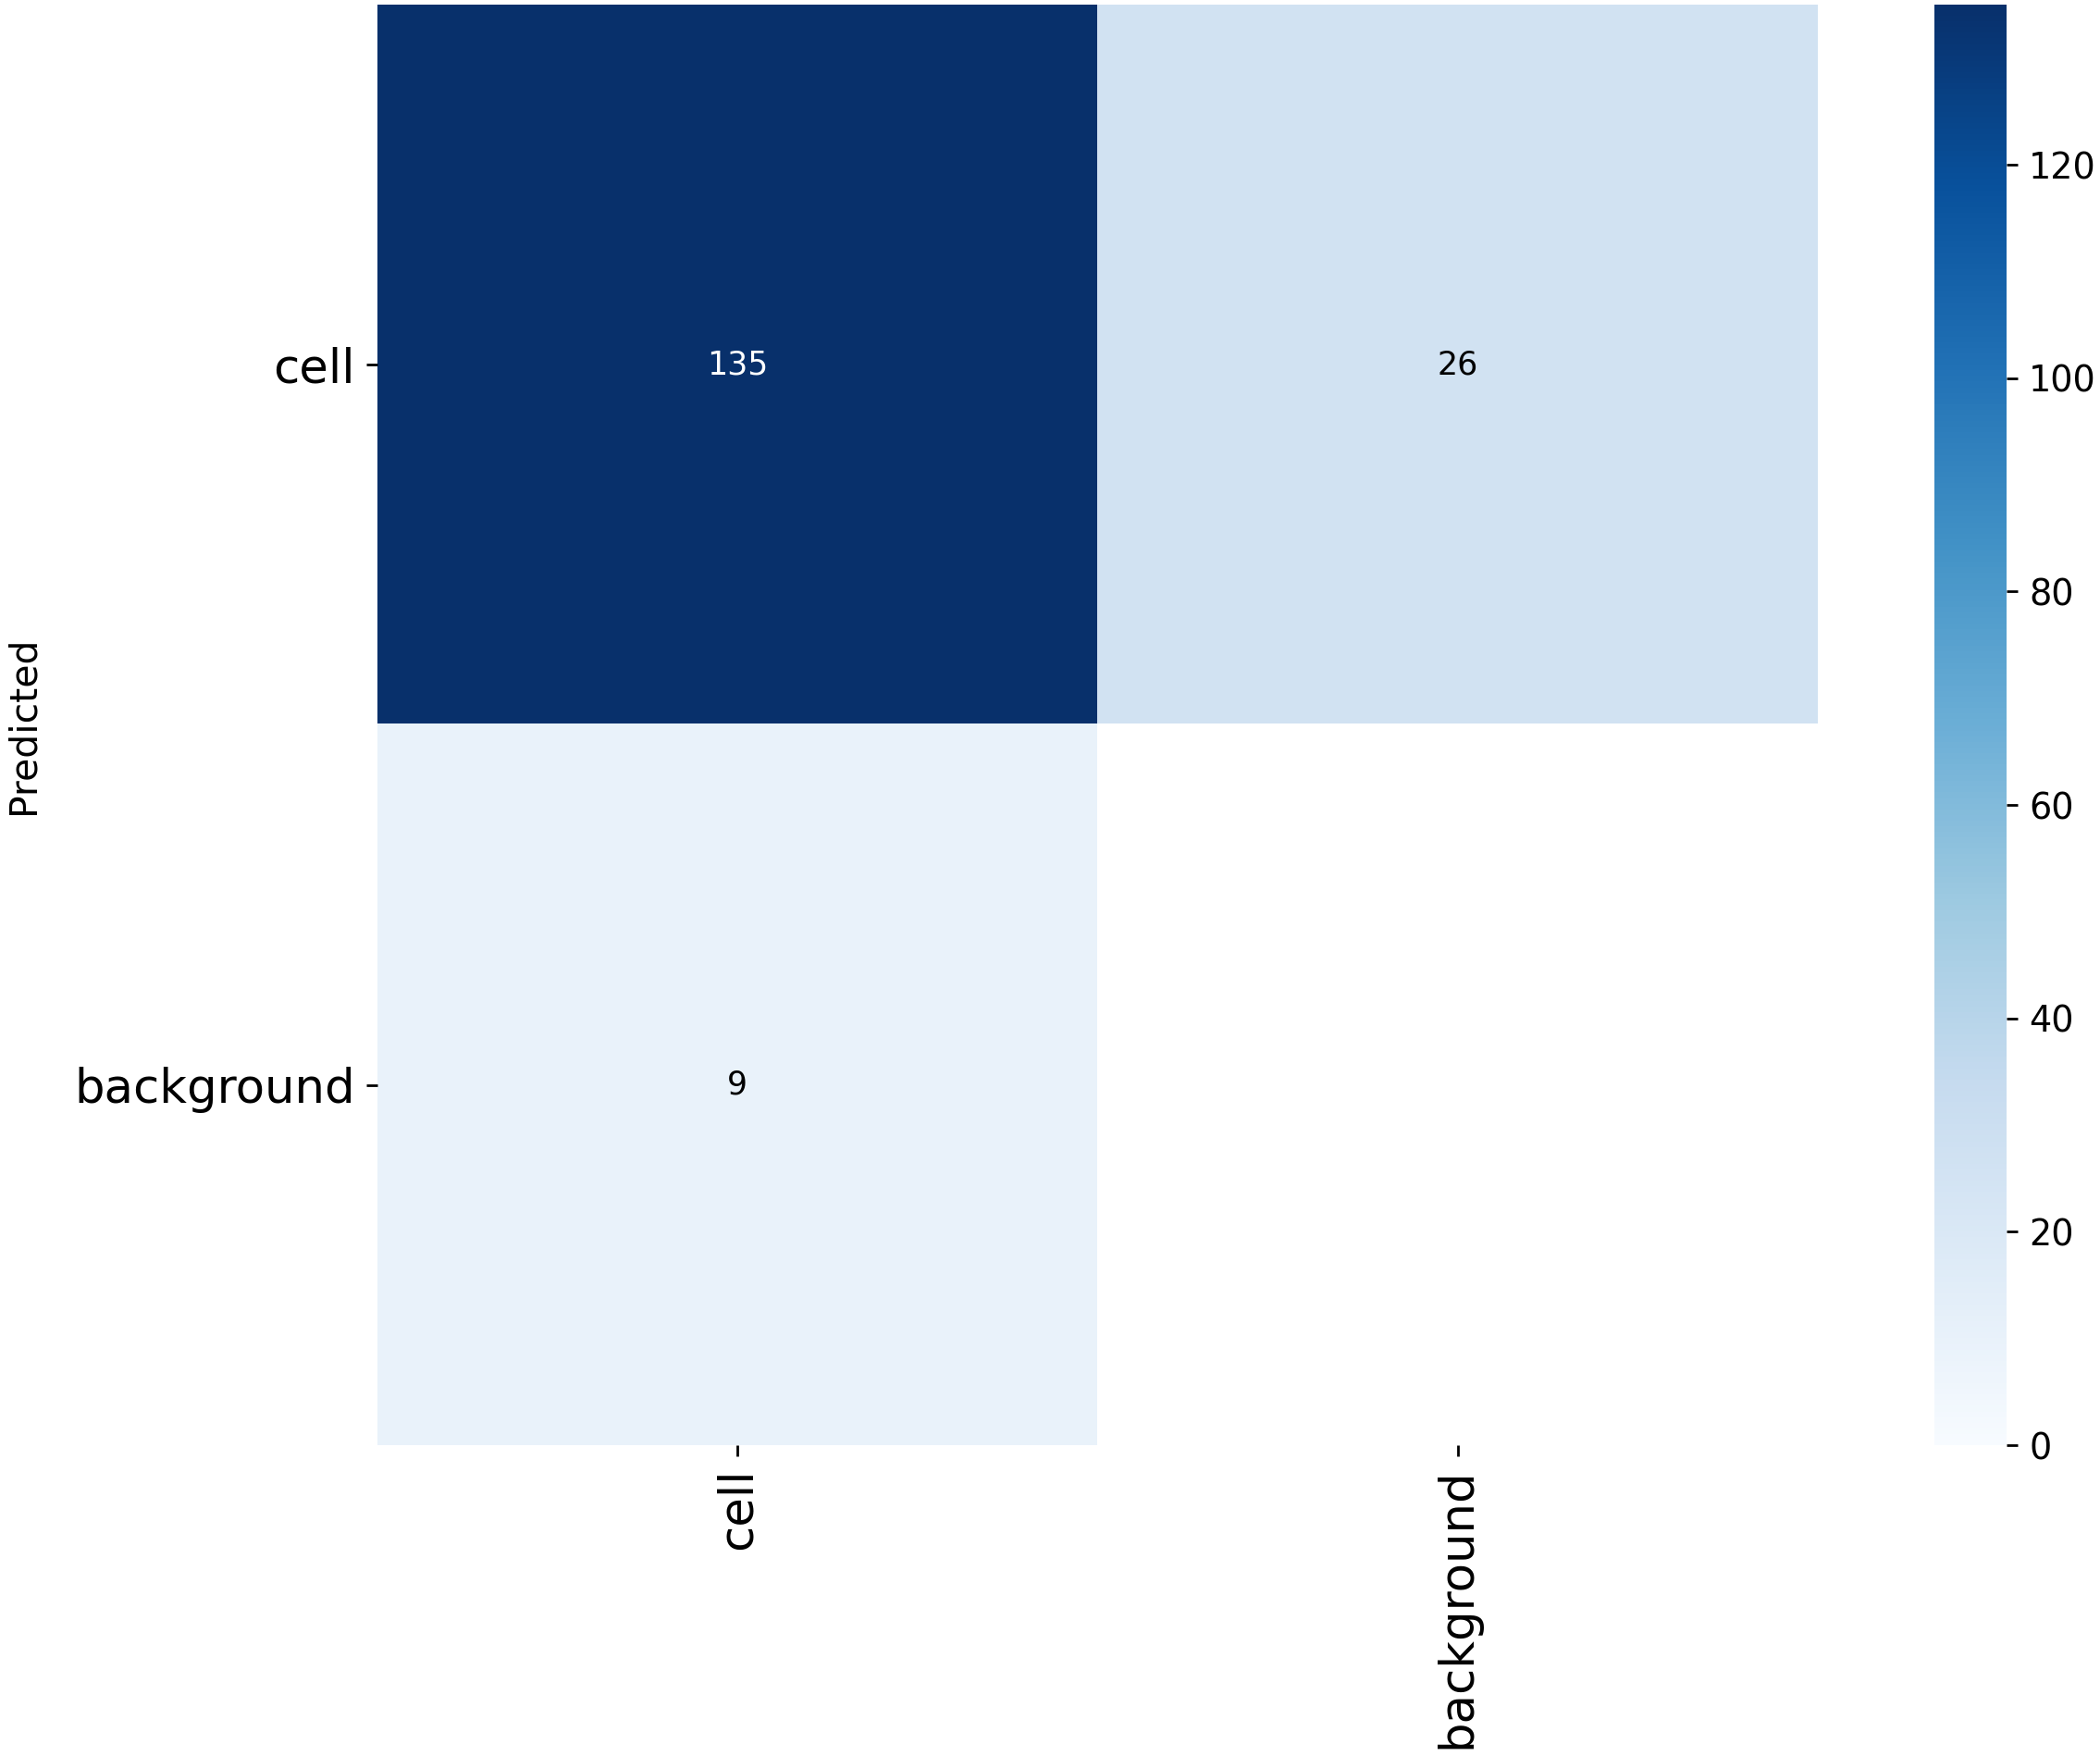
\includegraphics[height=5cm]{figuras/resultados experimentacion/custom/test2/confusion_matrix.png}
    \vspace{-0.3cm}
    \caption{\footnotesize \textit{custom}}
    \label{fig:confusion_custom_test2}
  \end{subfigure}
  \hfill
  \begin{subfigure}[b]{0.45\textwidth}
    \centering
    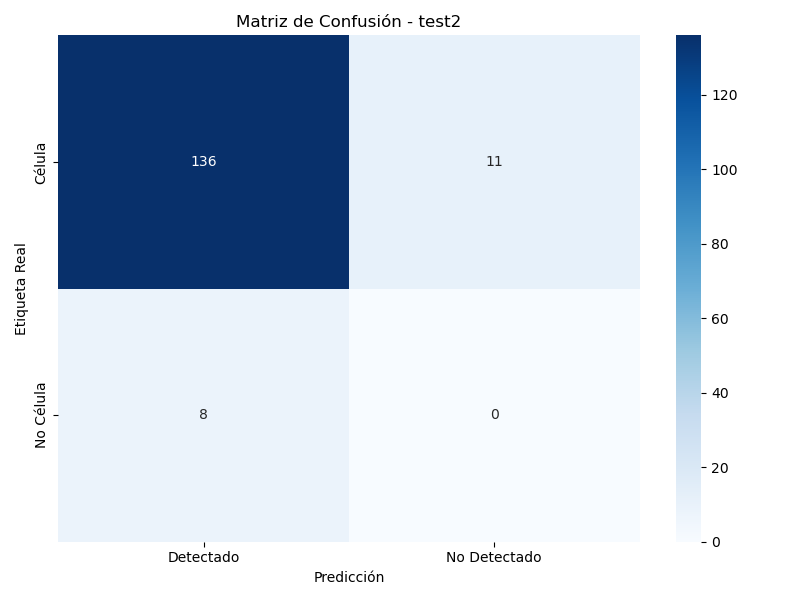
\includegraphics[height=5cm]{figuras/resultados experimentacion/ensemble/confusion_matrices/confusion_matrix_test2.png}
    \vspace{-0.3cm}
    \caption{\footnotesize \textit{ensemble}}
    \label{fig:confusion_ensemble_test2}
  \end{subfigure}
  
  \vspace{-0.2cm}
  \caption{Matrices de confusión para los modelos evaluados en test2}
  \label{fig:confusion_matrices_test2}
\end{figure}


% FIGURA PARA TEST3
\begin{figure}[H]
  \centering
  \vspace{-0.3cm}
  % Primera fila
  \begin{subfigure}[b]{0.45\textwidth}
    \centering
    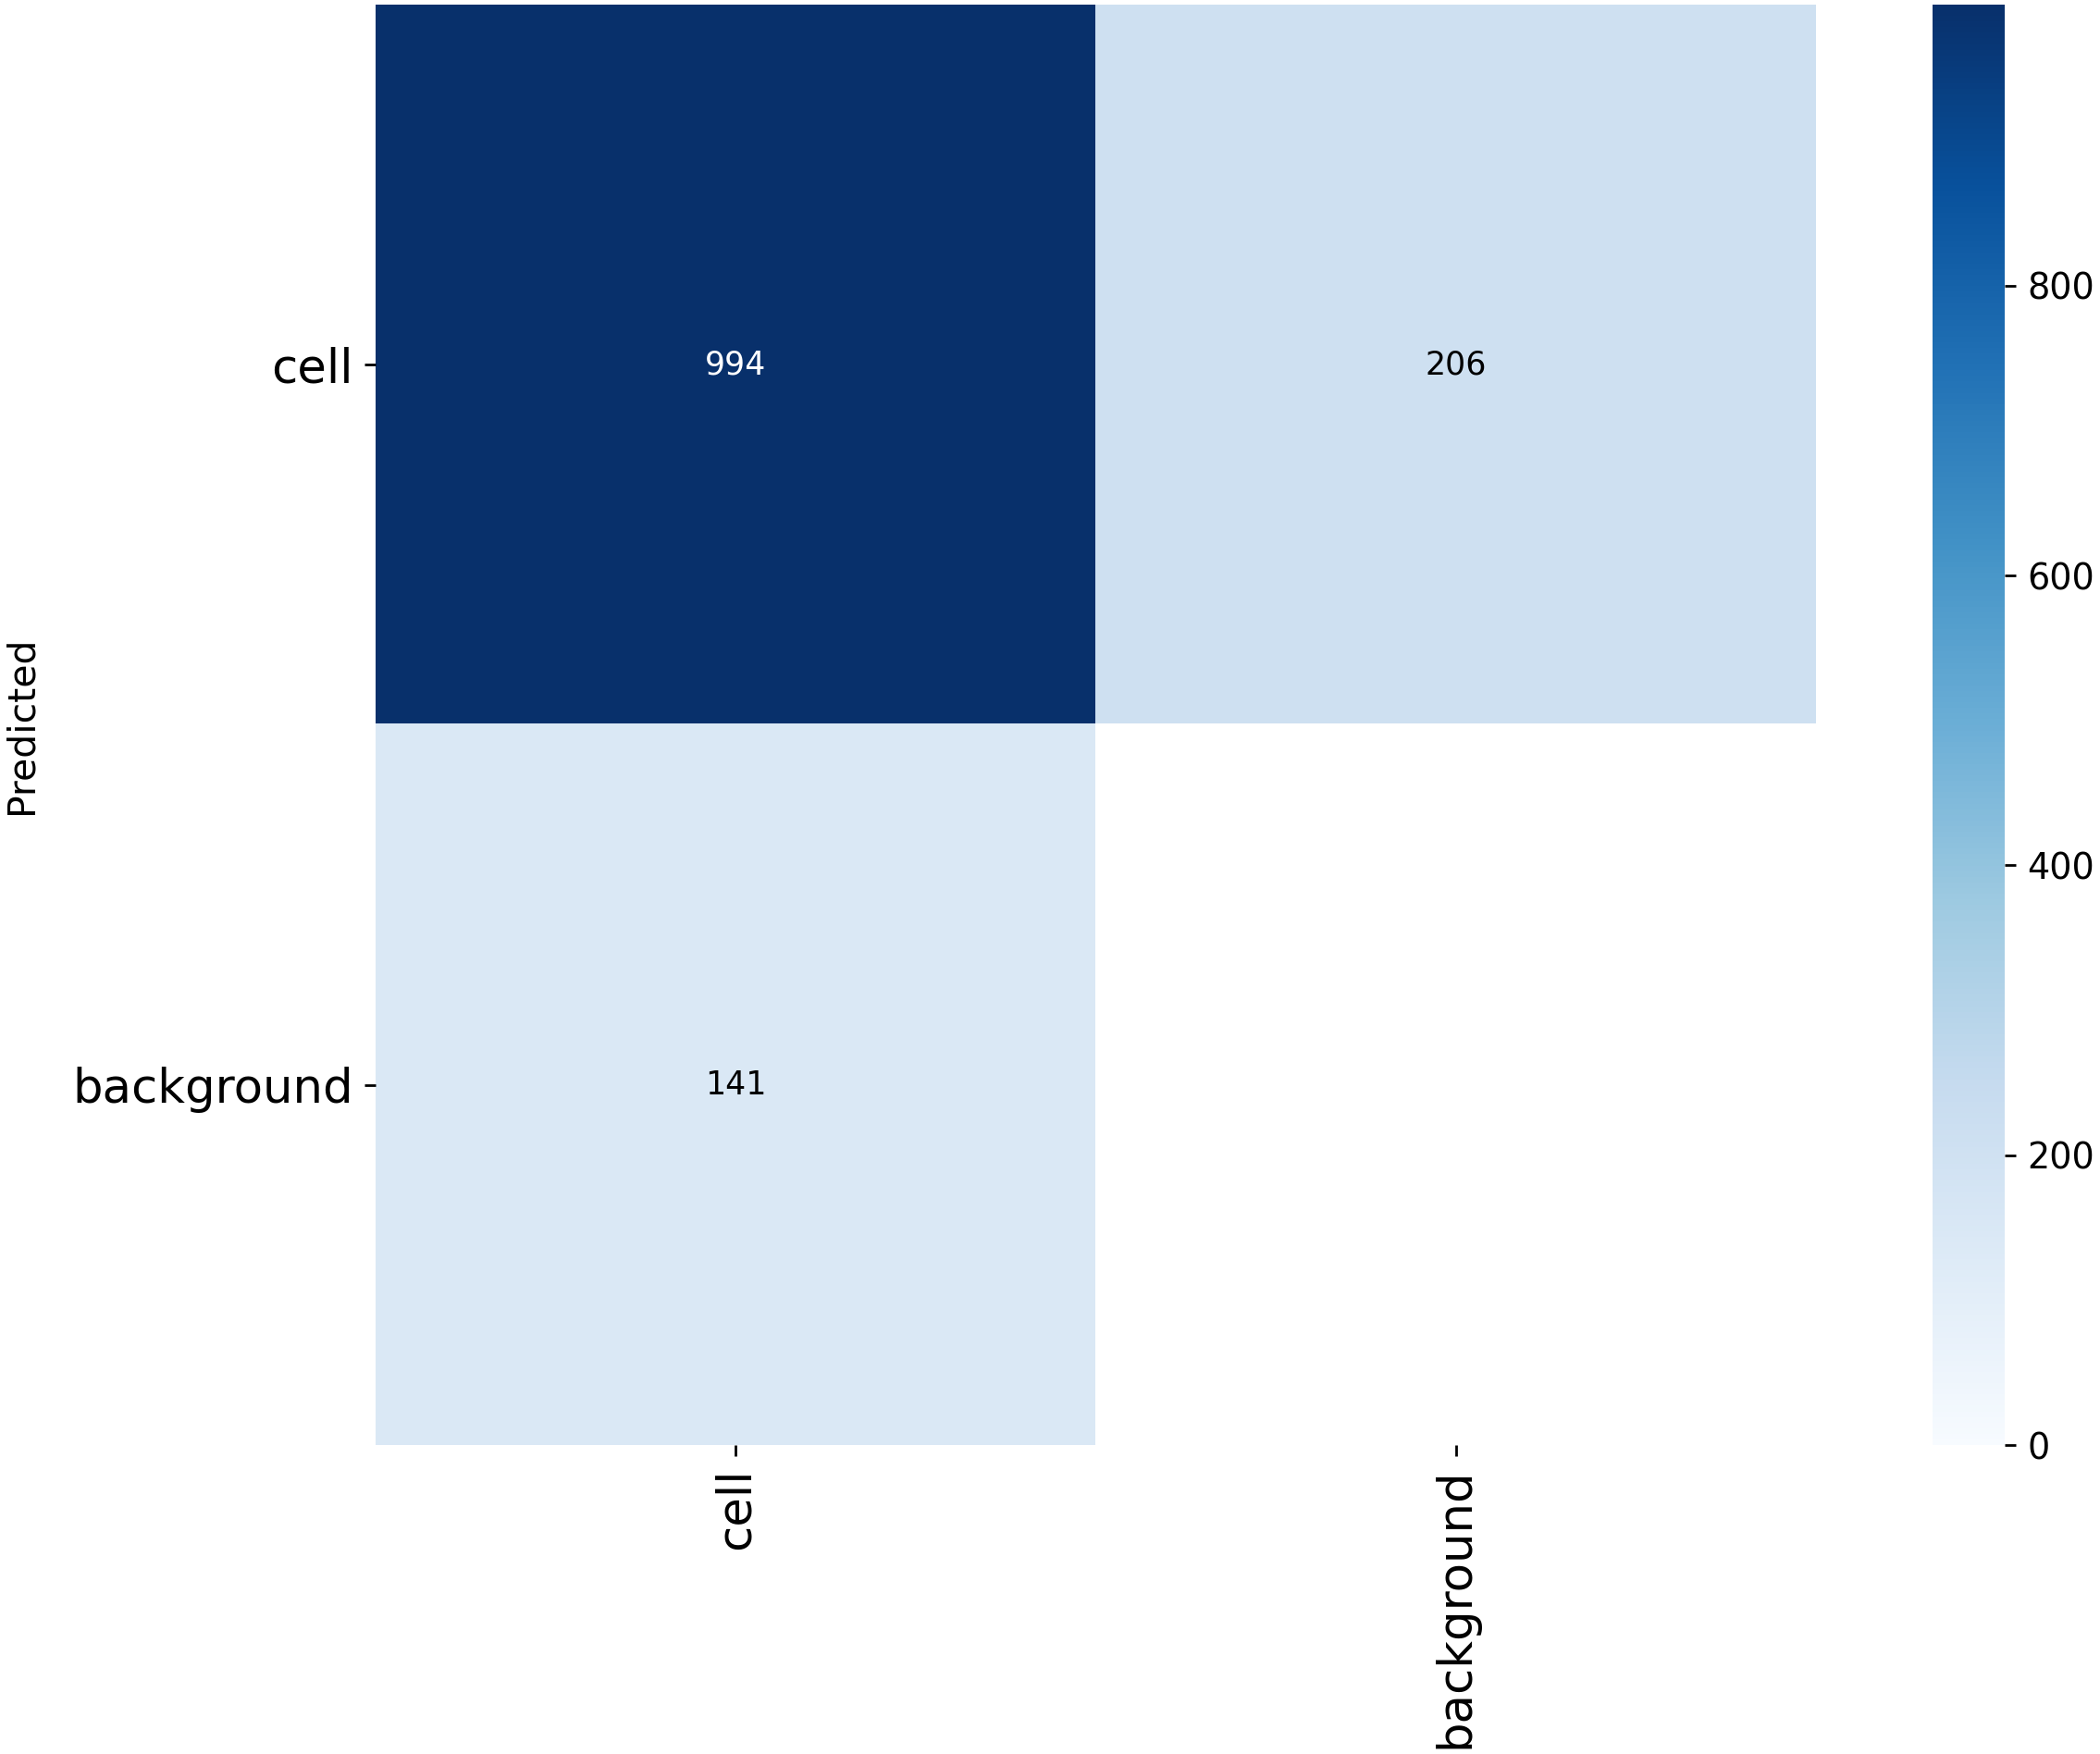
\includegraphics[height=5cm]{figuras/resultados experimentacion/yolov8s/test3/confusion_matrix.png}
    \vspace{-0.3cm}
    \caption{\footnotesize YOLOv8s}
    \label{fig:confusion_yolov8s_test3}
  \end{subfigure}
  \hfill
  \begin{subfigure}[b]{0.45\textwidth}
    \centering
    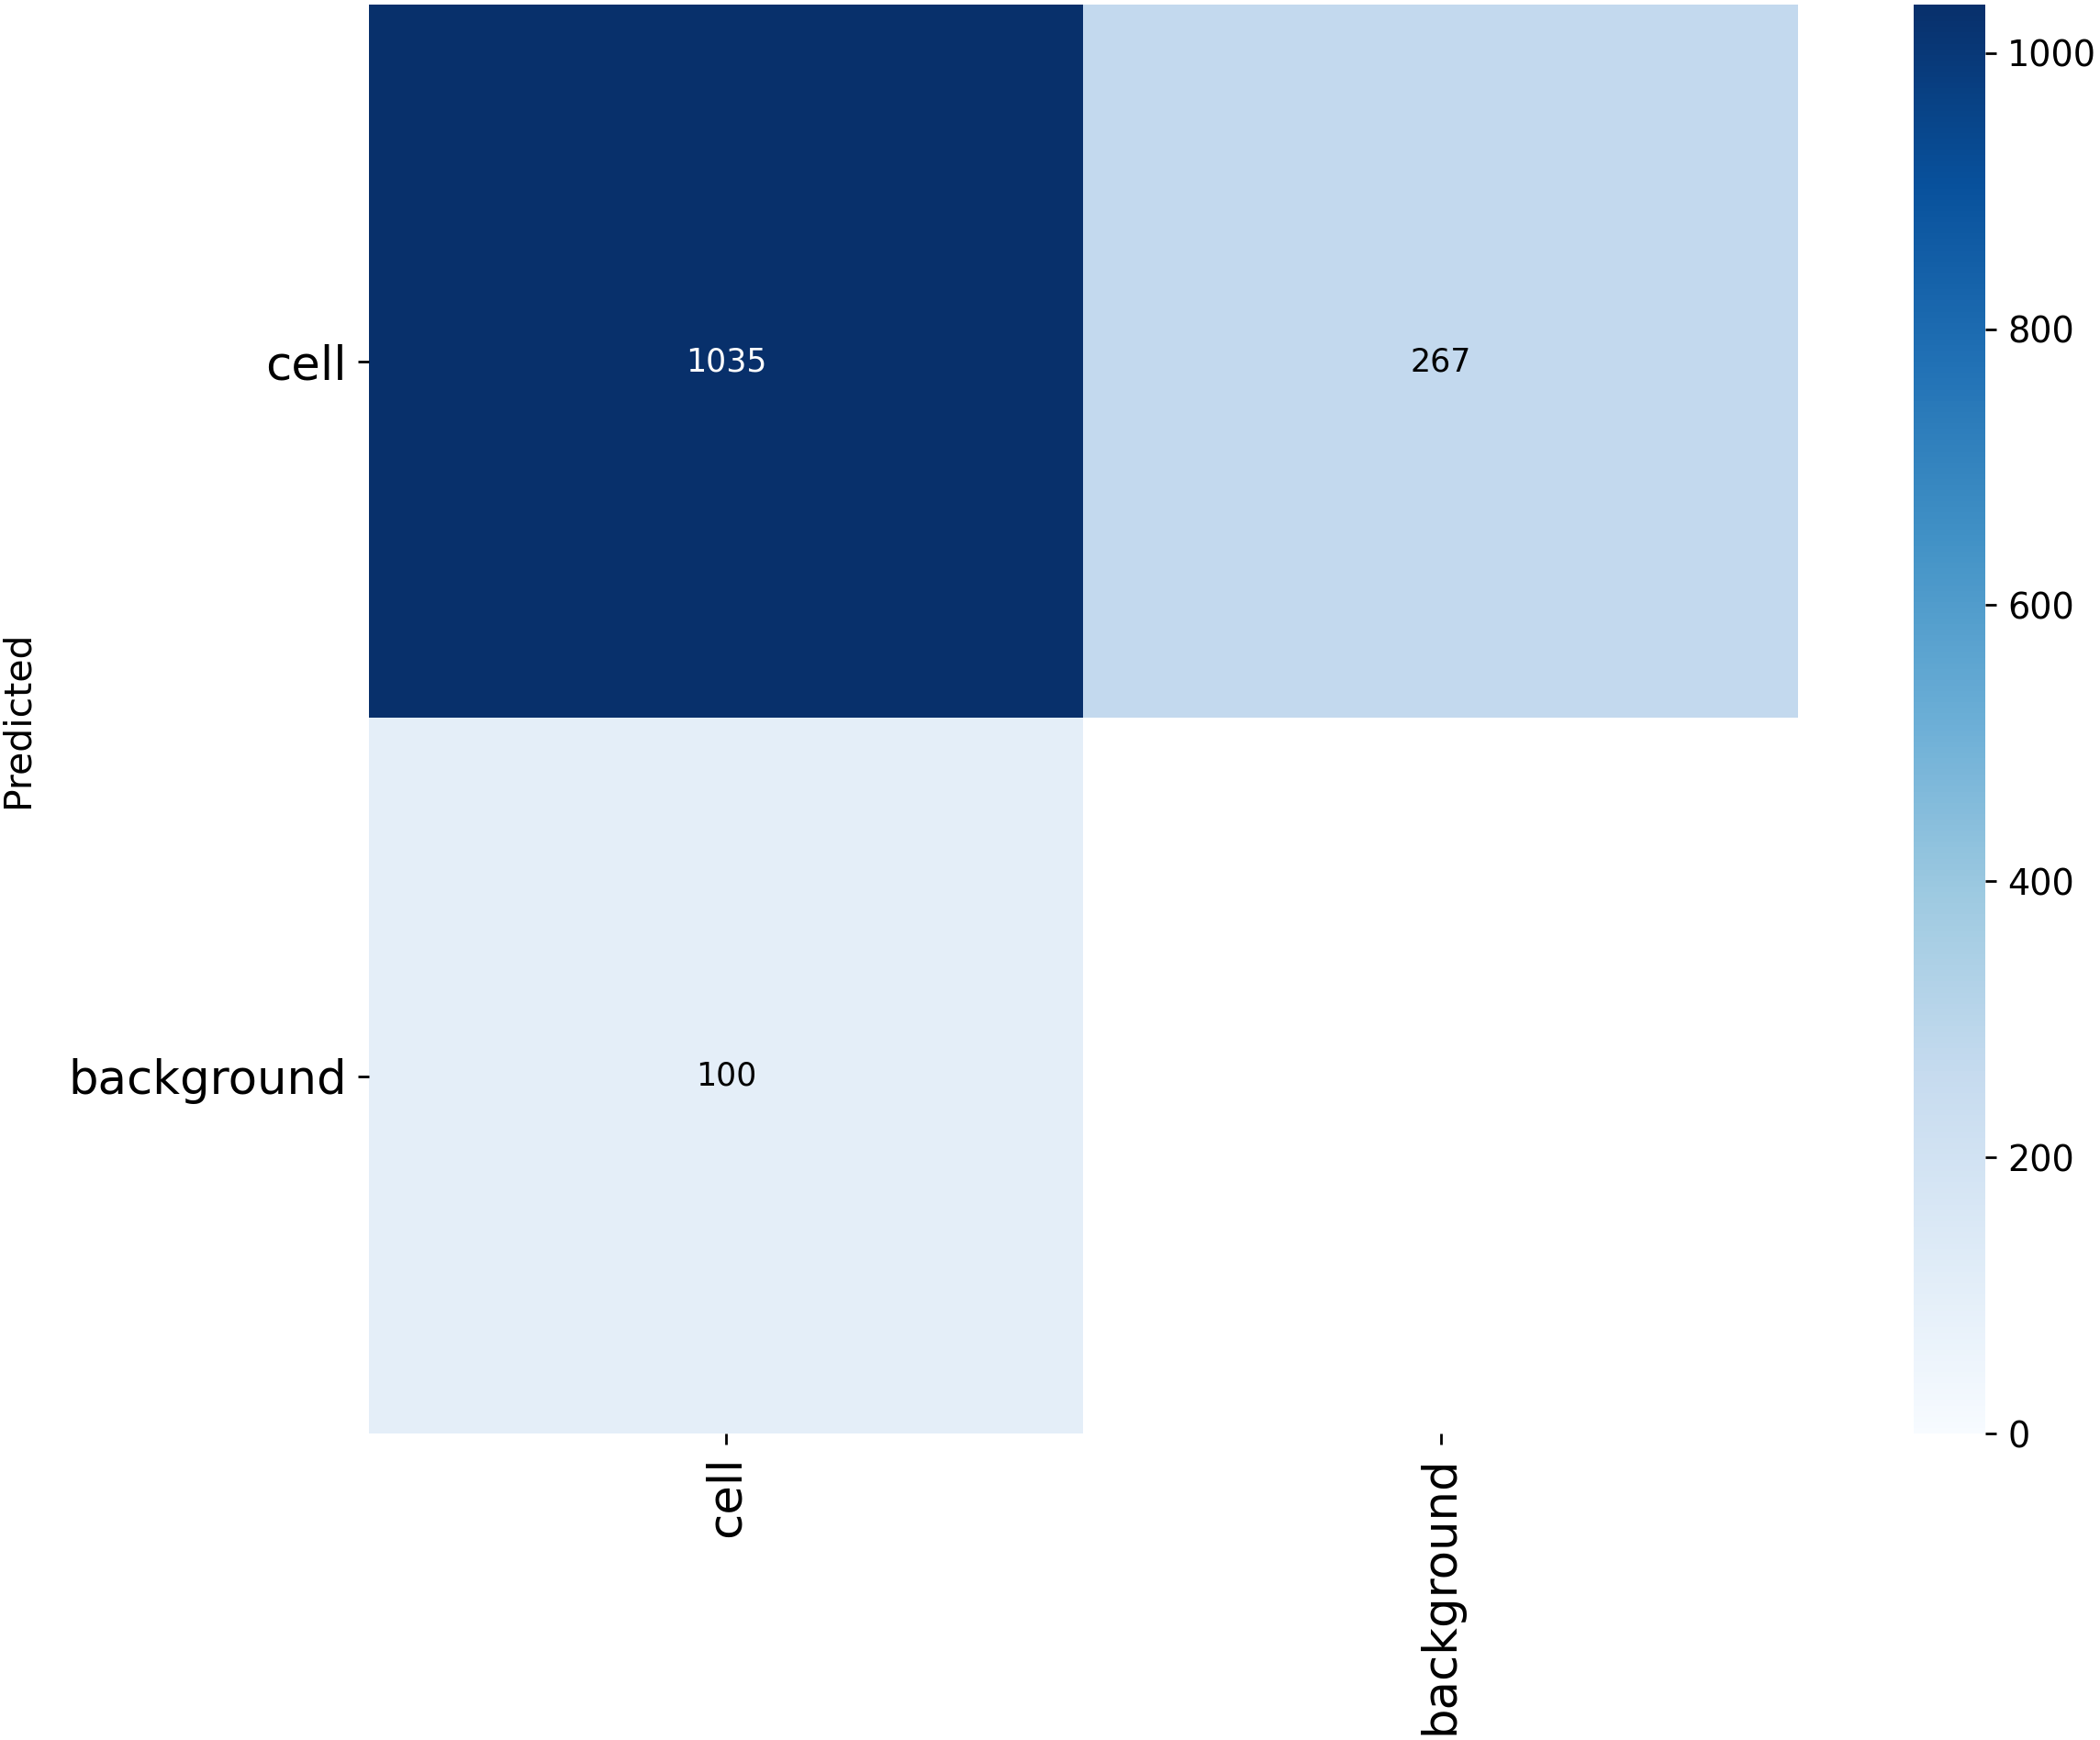
\includegraphics[height=5cm]{figuras/resultados experimentacion/yolov9s/test3/confusion_matrix.png}
    \vspace{-0.3cm}
    \caption{\footnotesize YOLOv9s}
    \label{fig:confusion_yolov9s_test3}
  \end{subfigure}
  
  \vspace{0.1cm}
  % Segunda fila
  \begin{subfigure}[b]{0.45\textwidth}
    \centering
    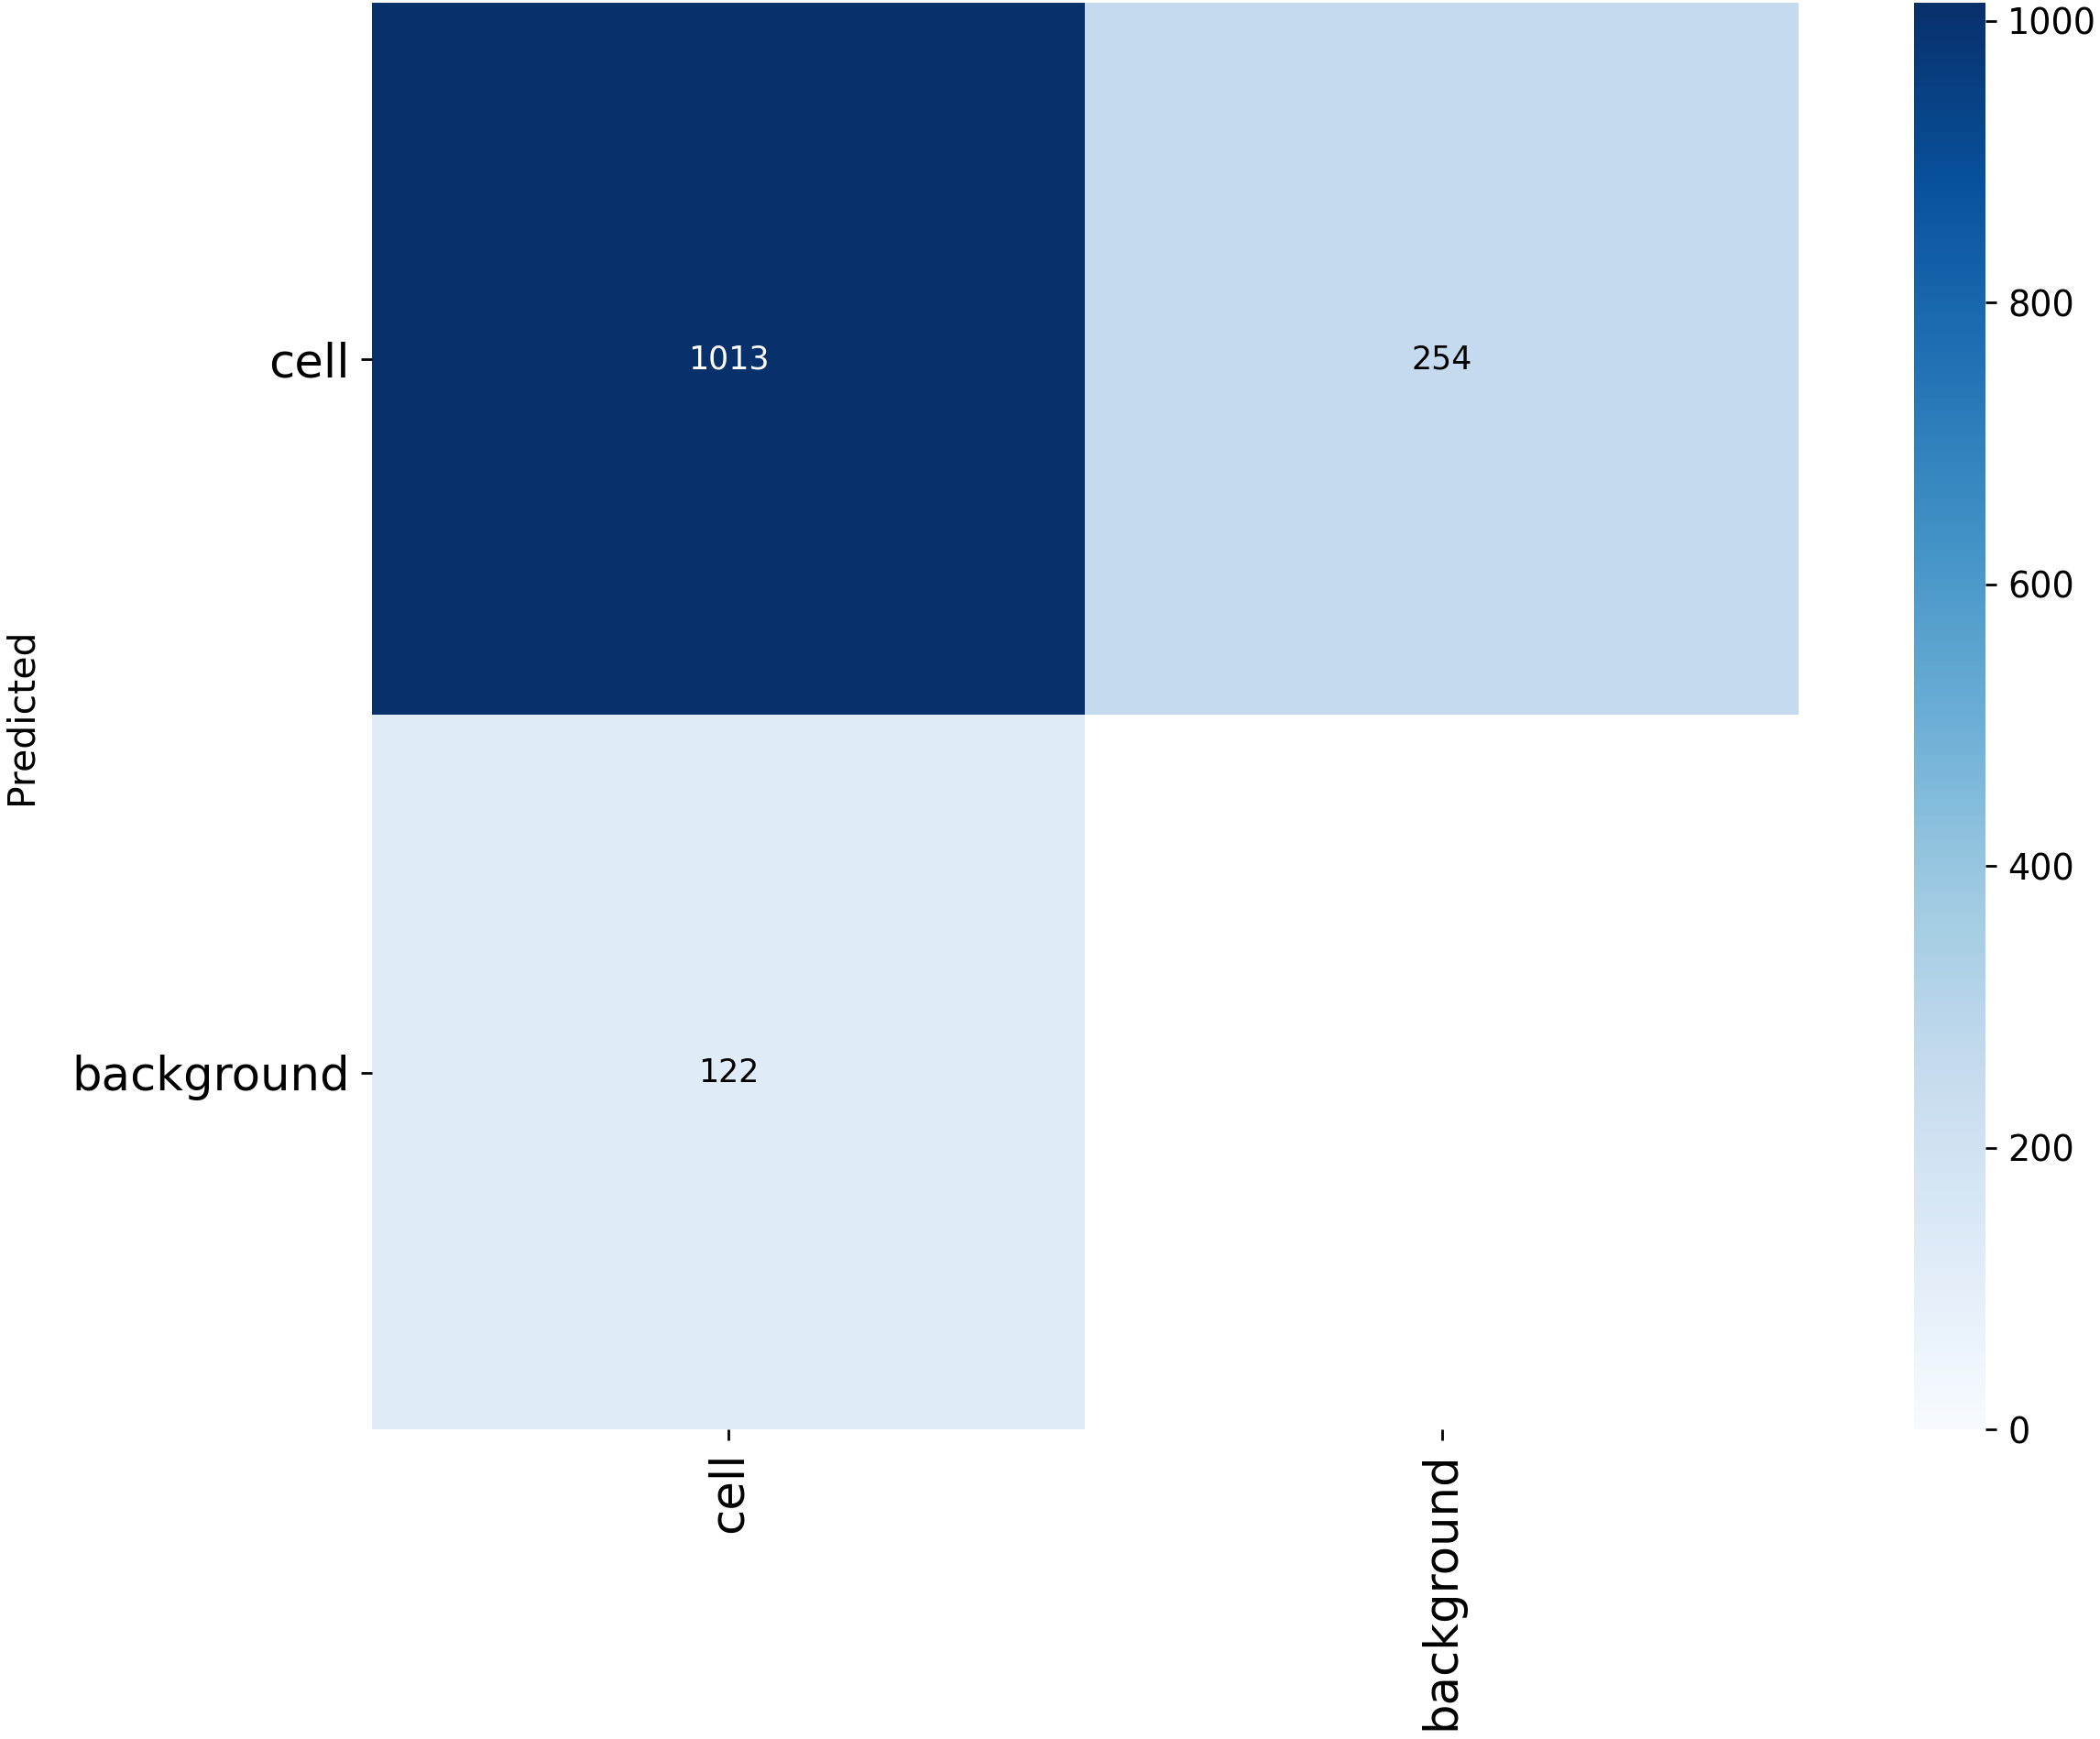
\includegraphics[height=5cm]{figuras/resultados experimentacion/yolov10s/test3/confusion_matrix.png}
    \vspace{-0.3cm}
    \caption{\footnotesize YOLOv10s}
    \label{fig:confusion_yolov10s_test3}
  \end{subfigure}
  \hfill
  \begin{subfigure}[b]{0.45\textwidth}
    \centering
    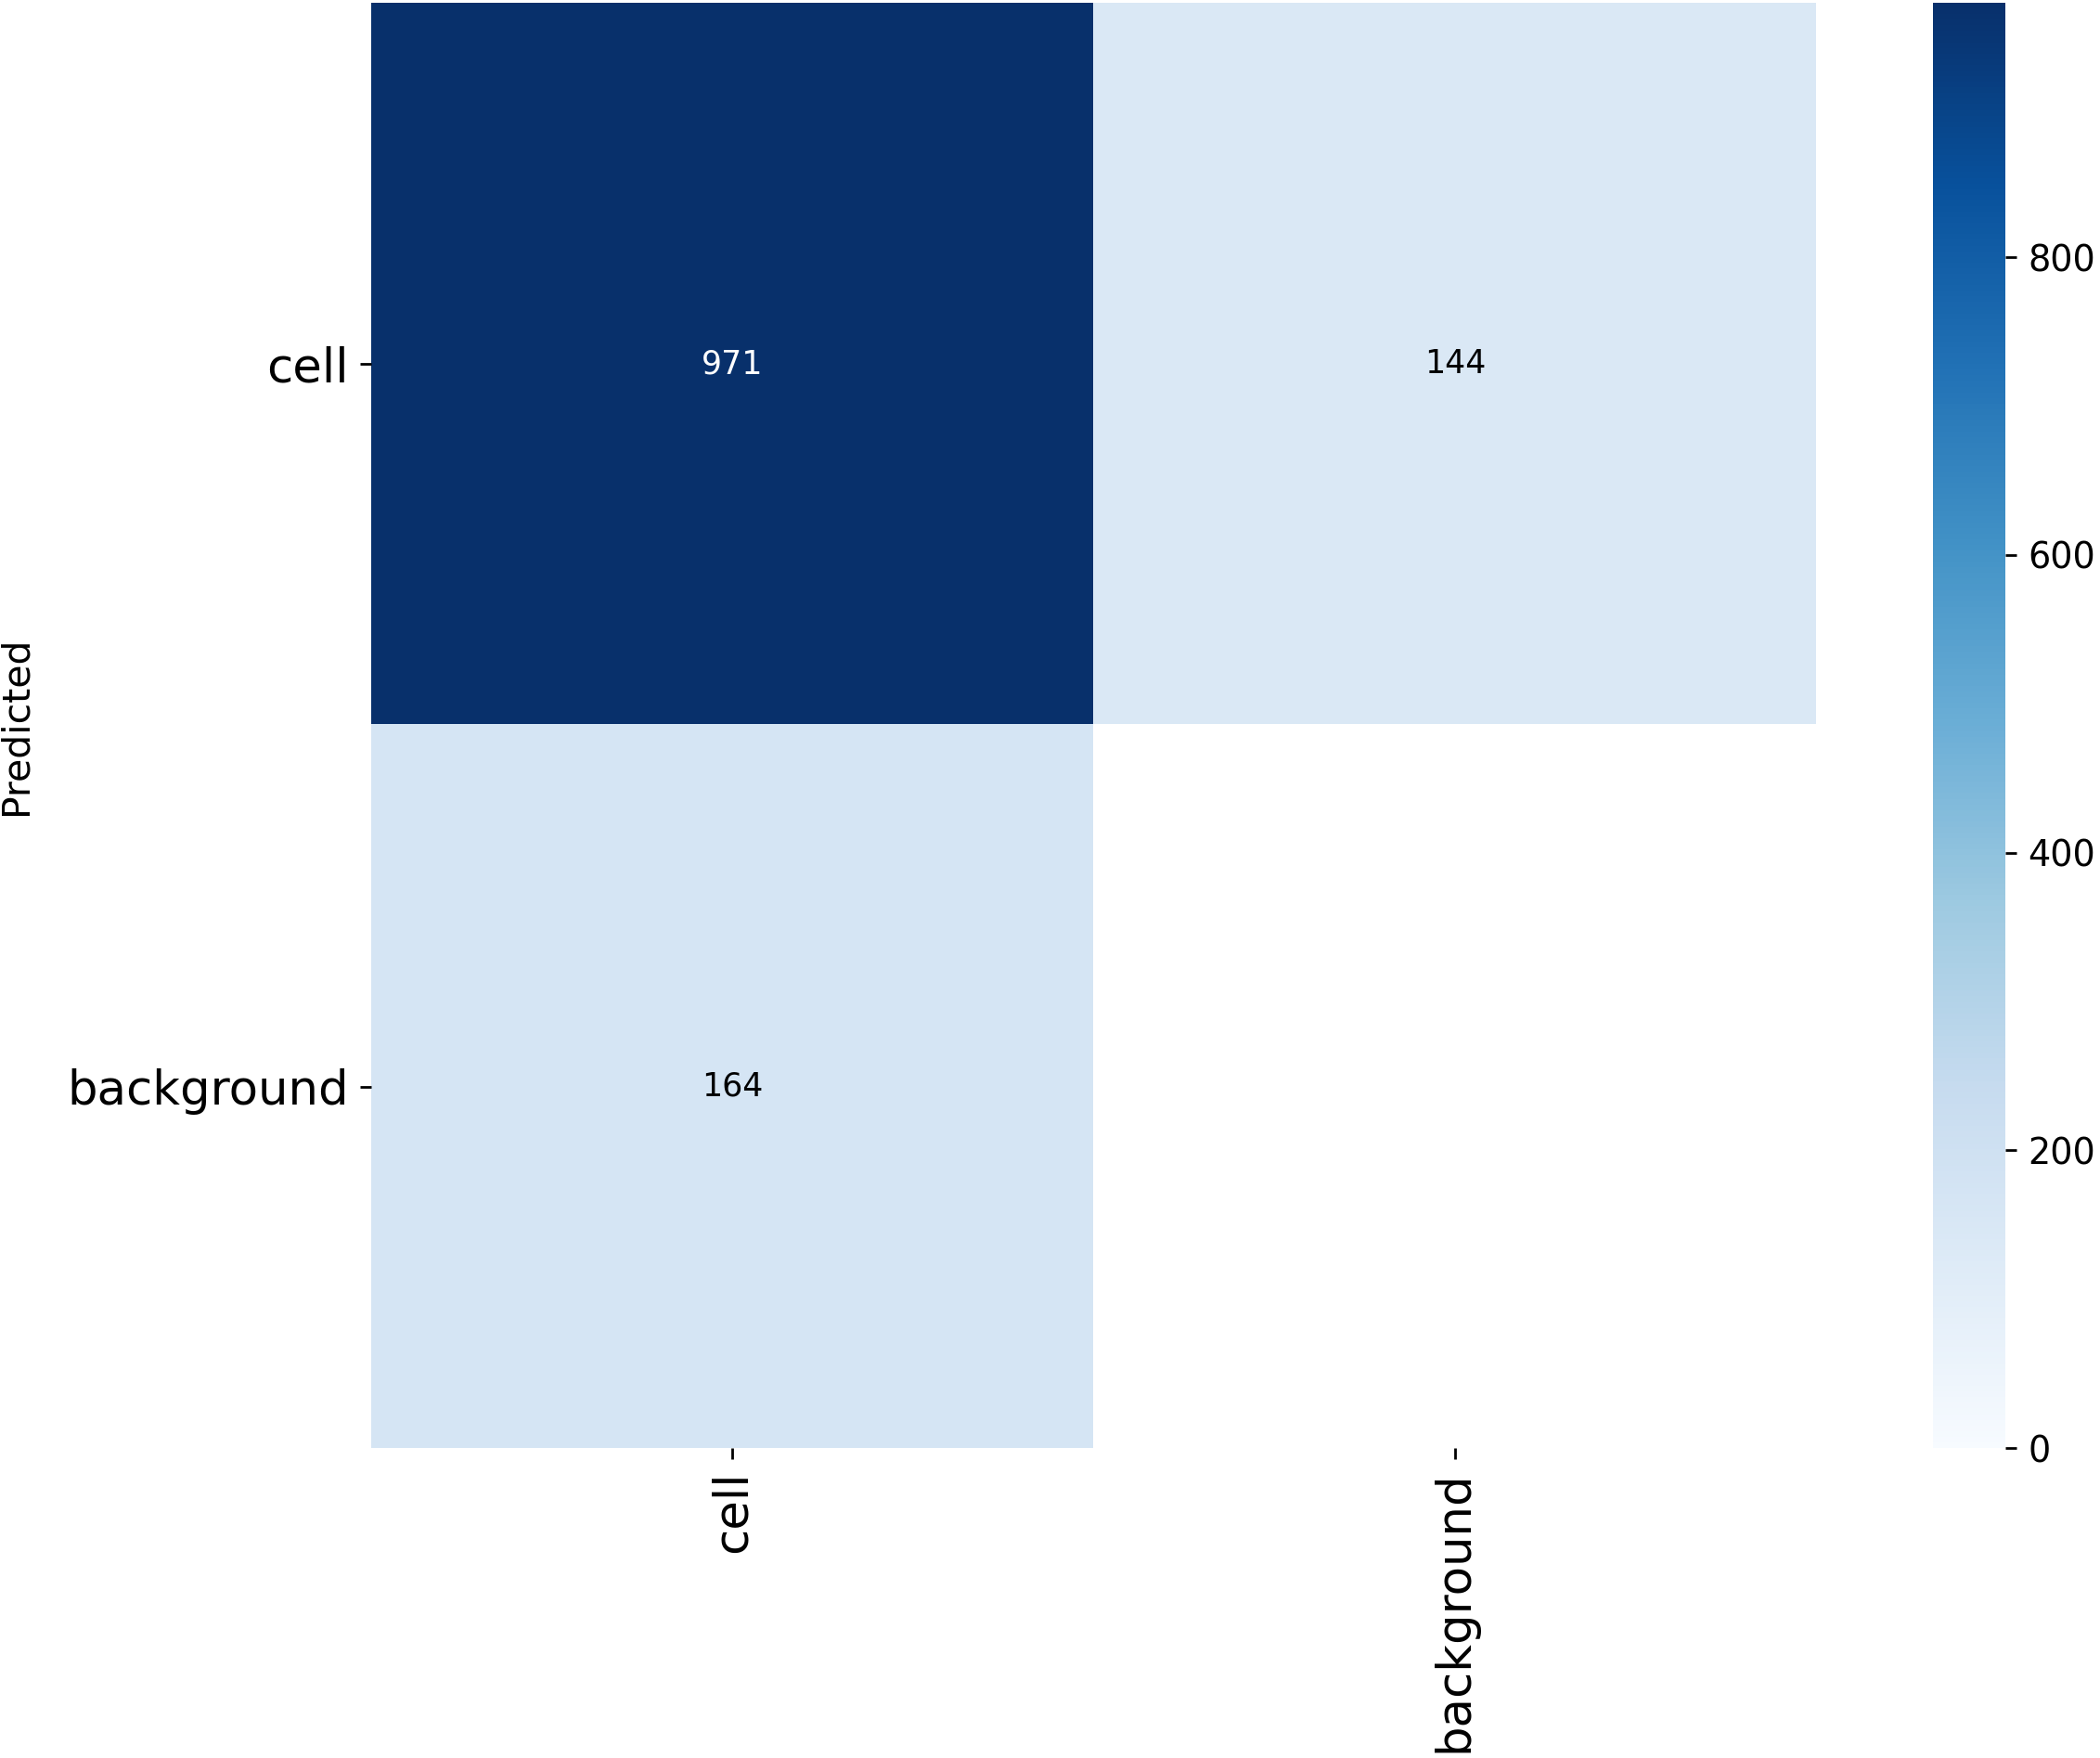
\includegraphics[height=5cm]{figuras/resultados experimentacion/yolov11s/test3/confusion_matrix.png}
    \vspace{-0.3cm}
    \caption{\footnotesize YOLOv11s}
    \label{fig:confusion_yolov11s_test3}
  \end{subfigure}
  
  \vspace{0.1cm}
  % Tercera fila
  \begin{subfigure}[b]{0.45\textwidth}
    \centering
    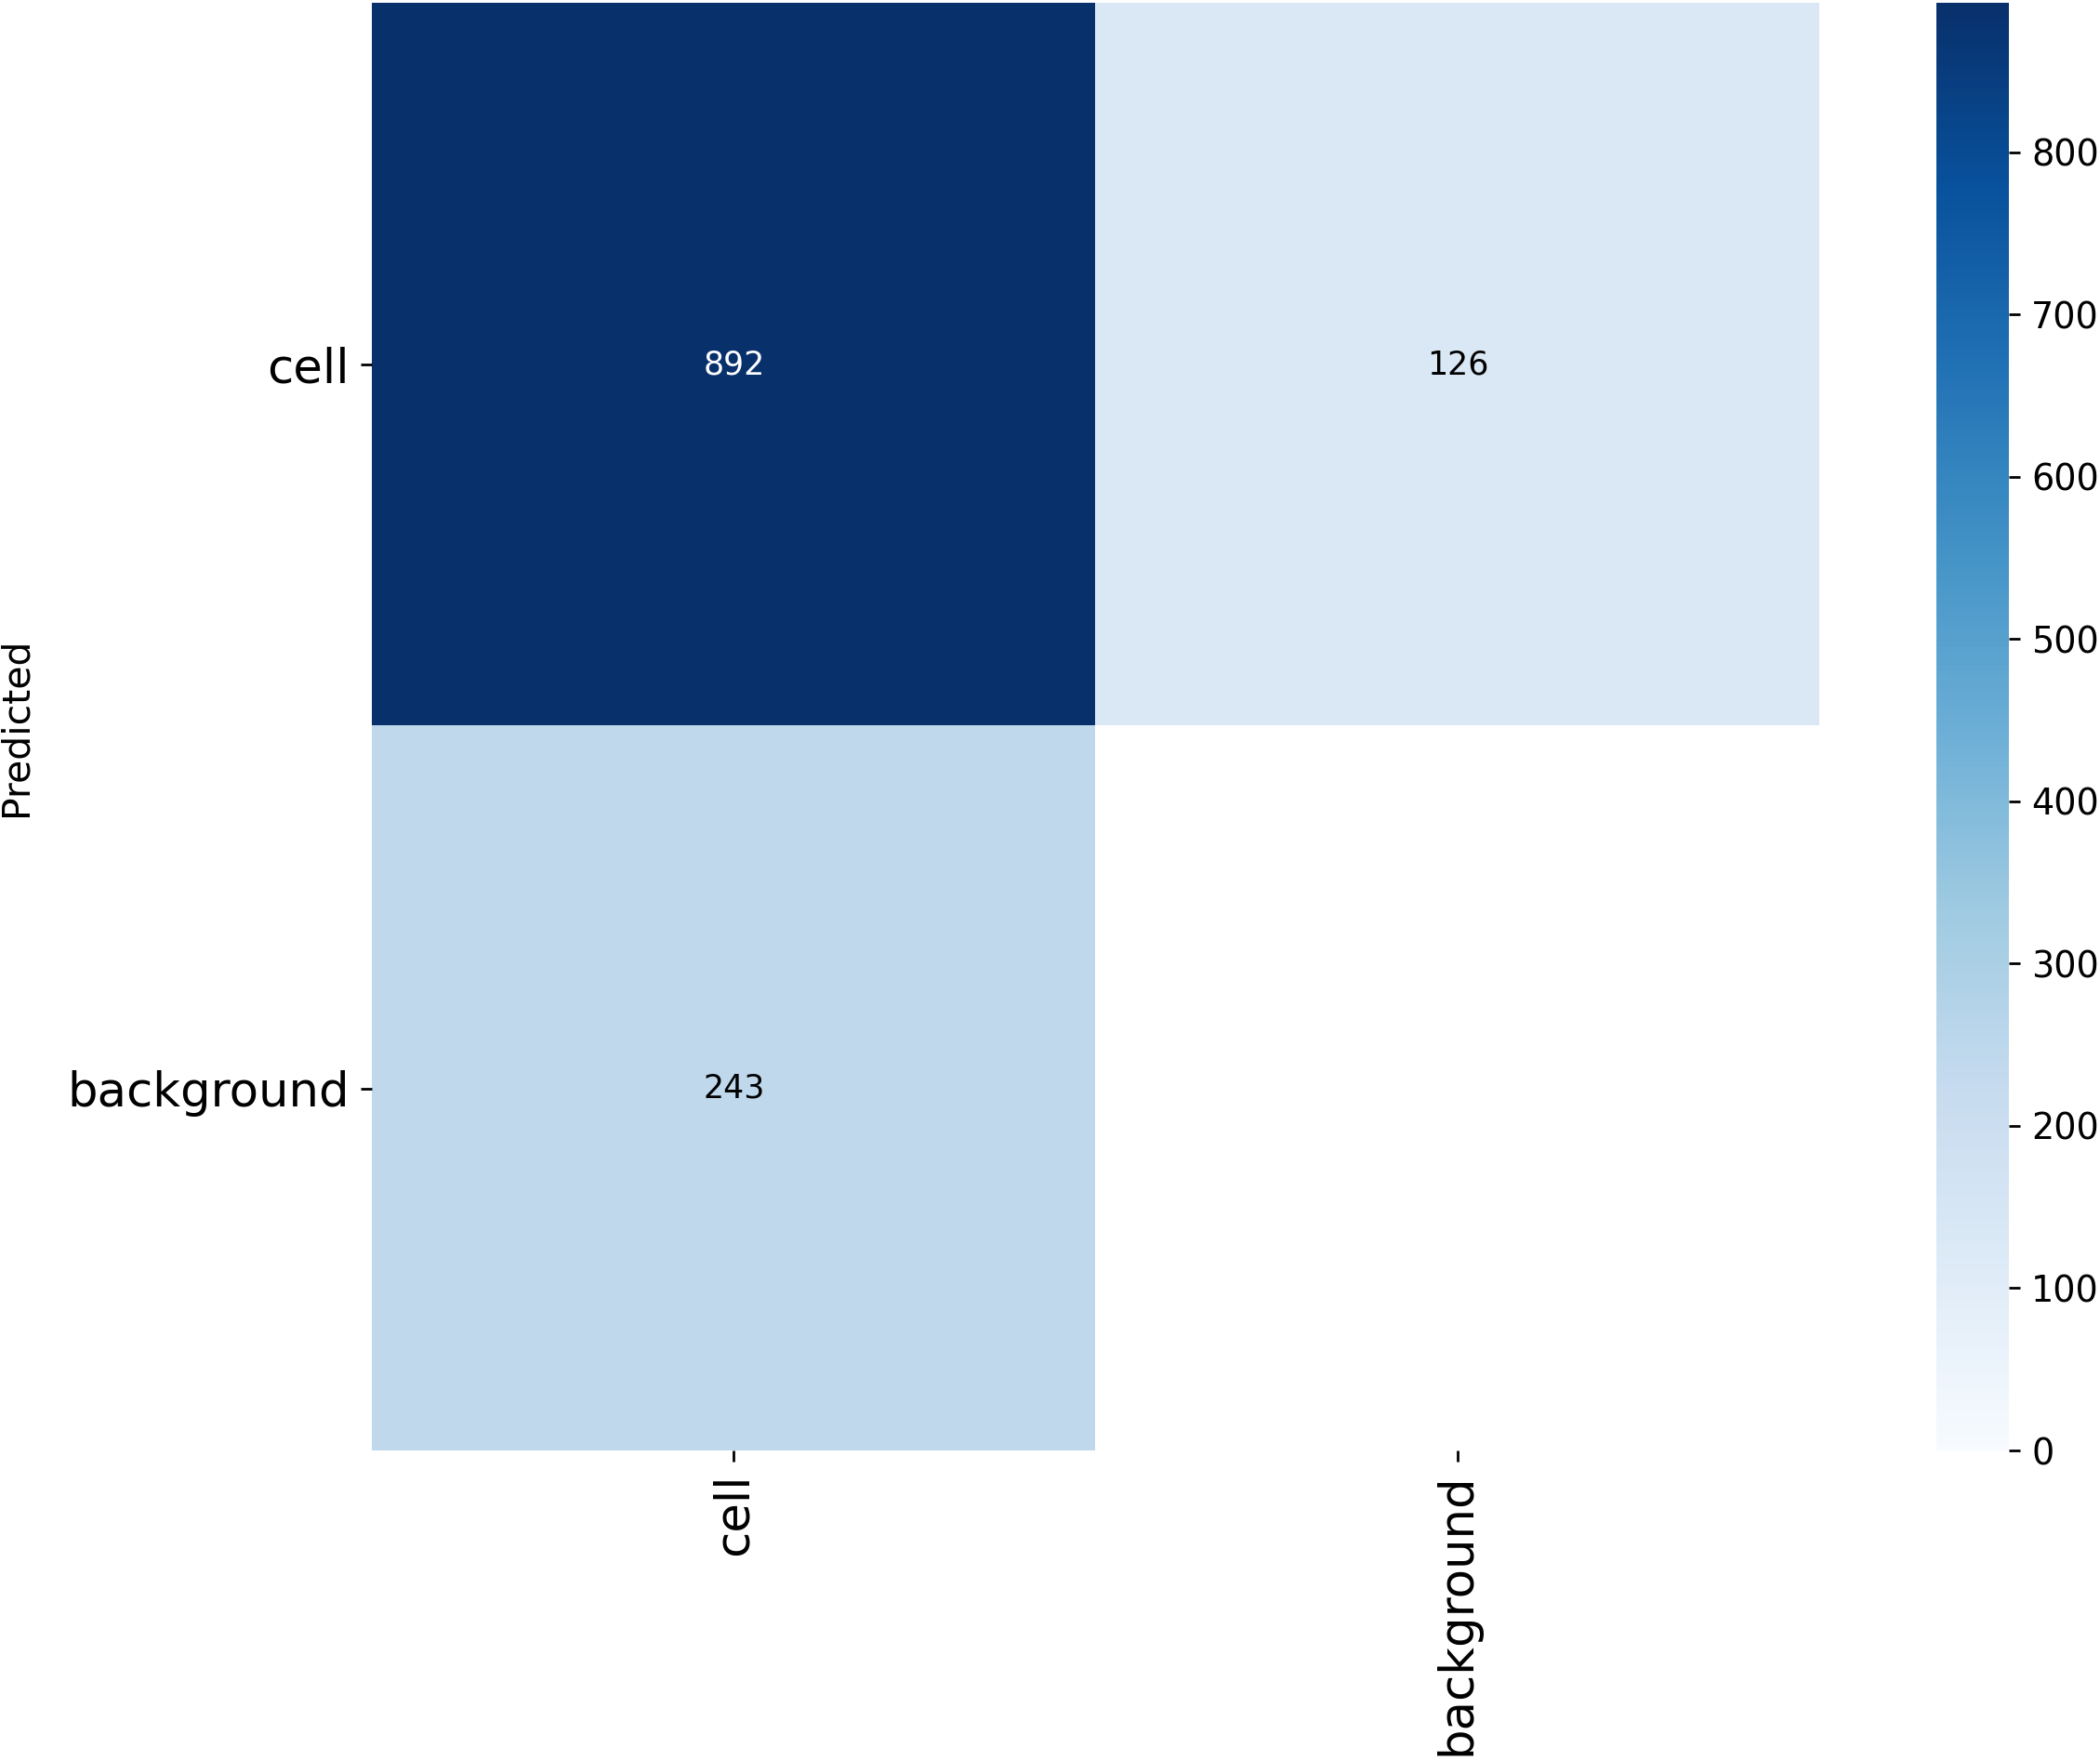
\includegraphics[height=5cm]{figuras/resultados experimentacion/yolov12s/test3/confusion_matrix.png}
    \vspace{-0.3cm}
    \caption{\footnotesize YOLOv12s}
    \label{fig:confusion_yolov12s_test3}
  \end{subfigure}
  \hfill
  \begin{subfigure}[b]{0.45\textwidth}
    \centering
    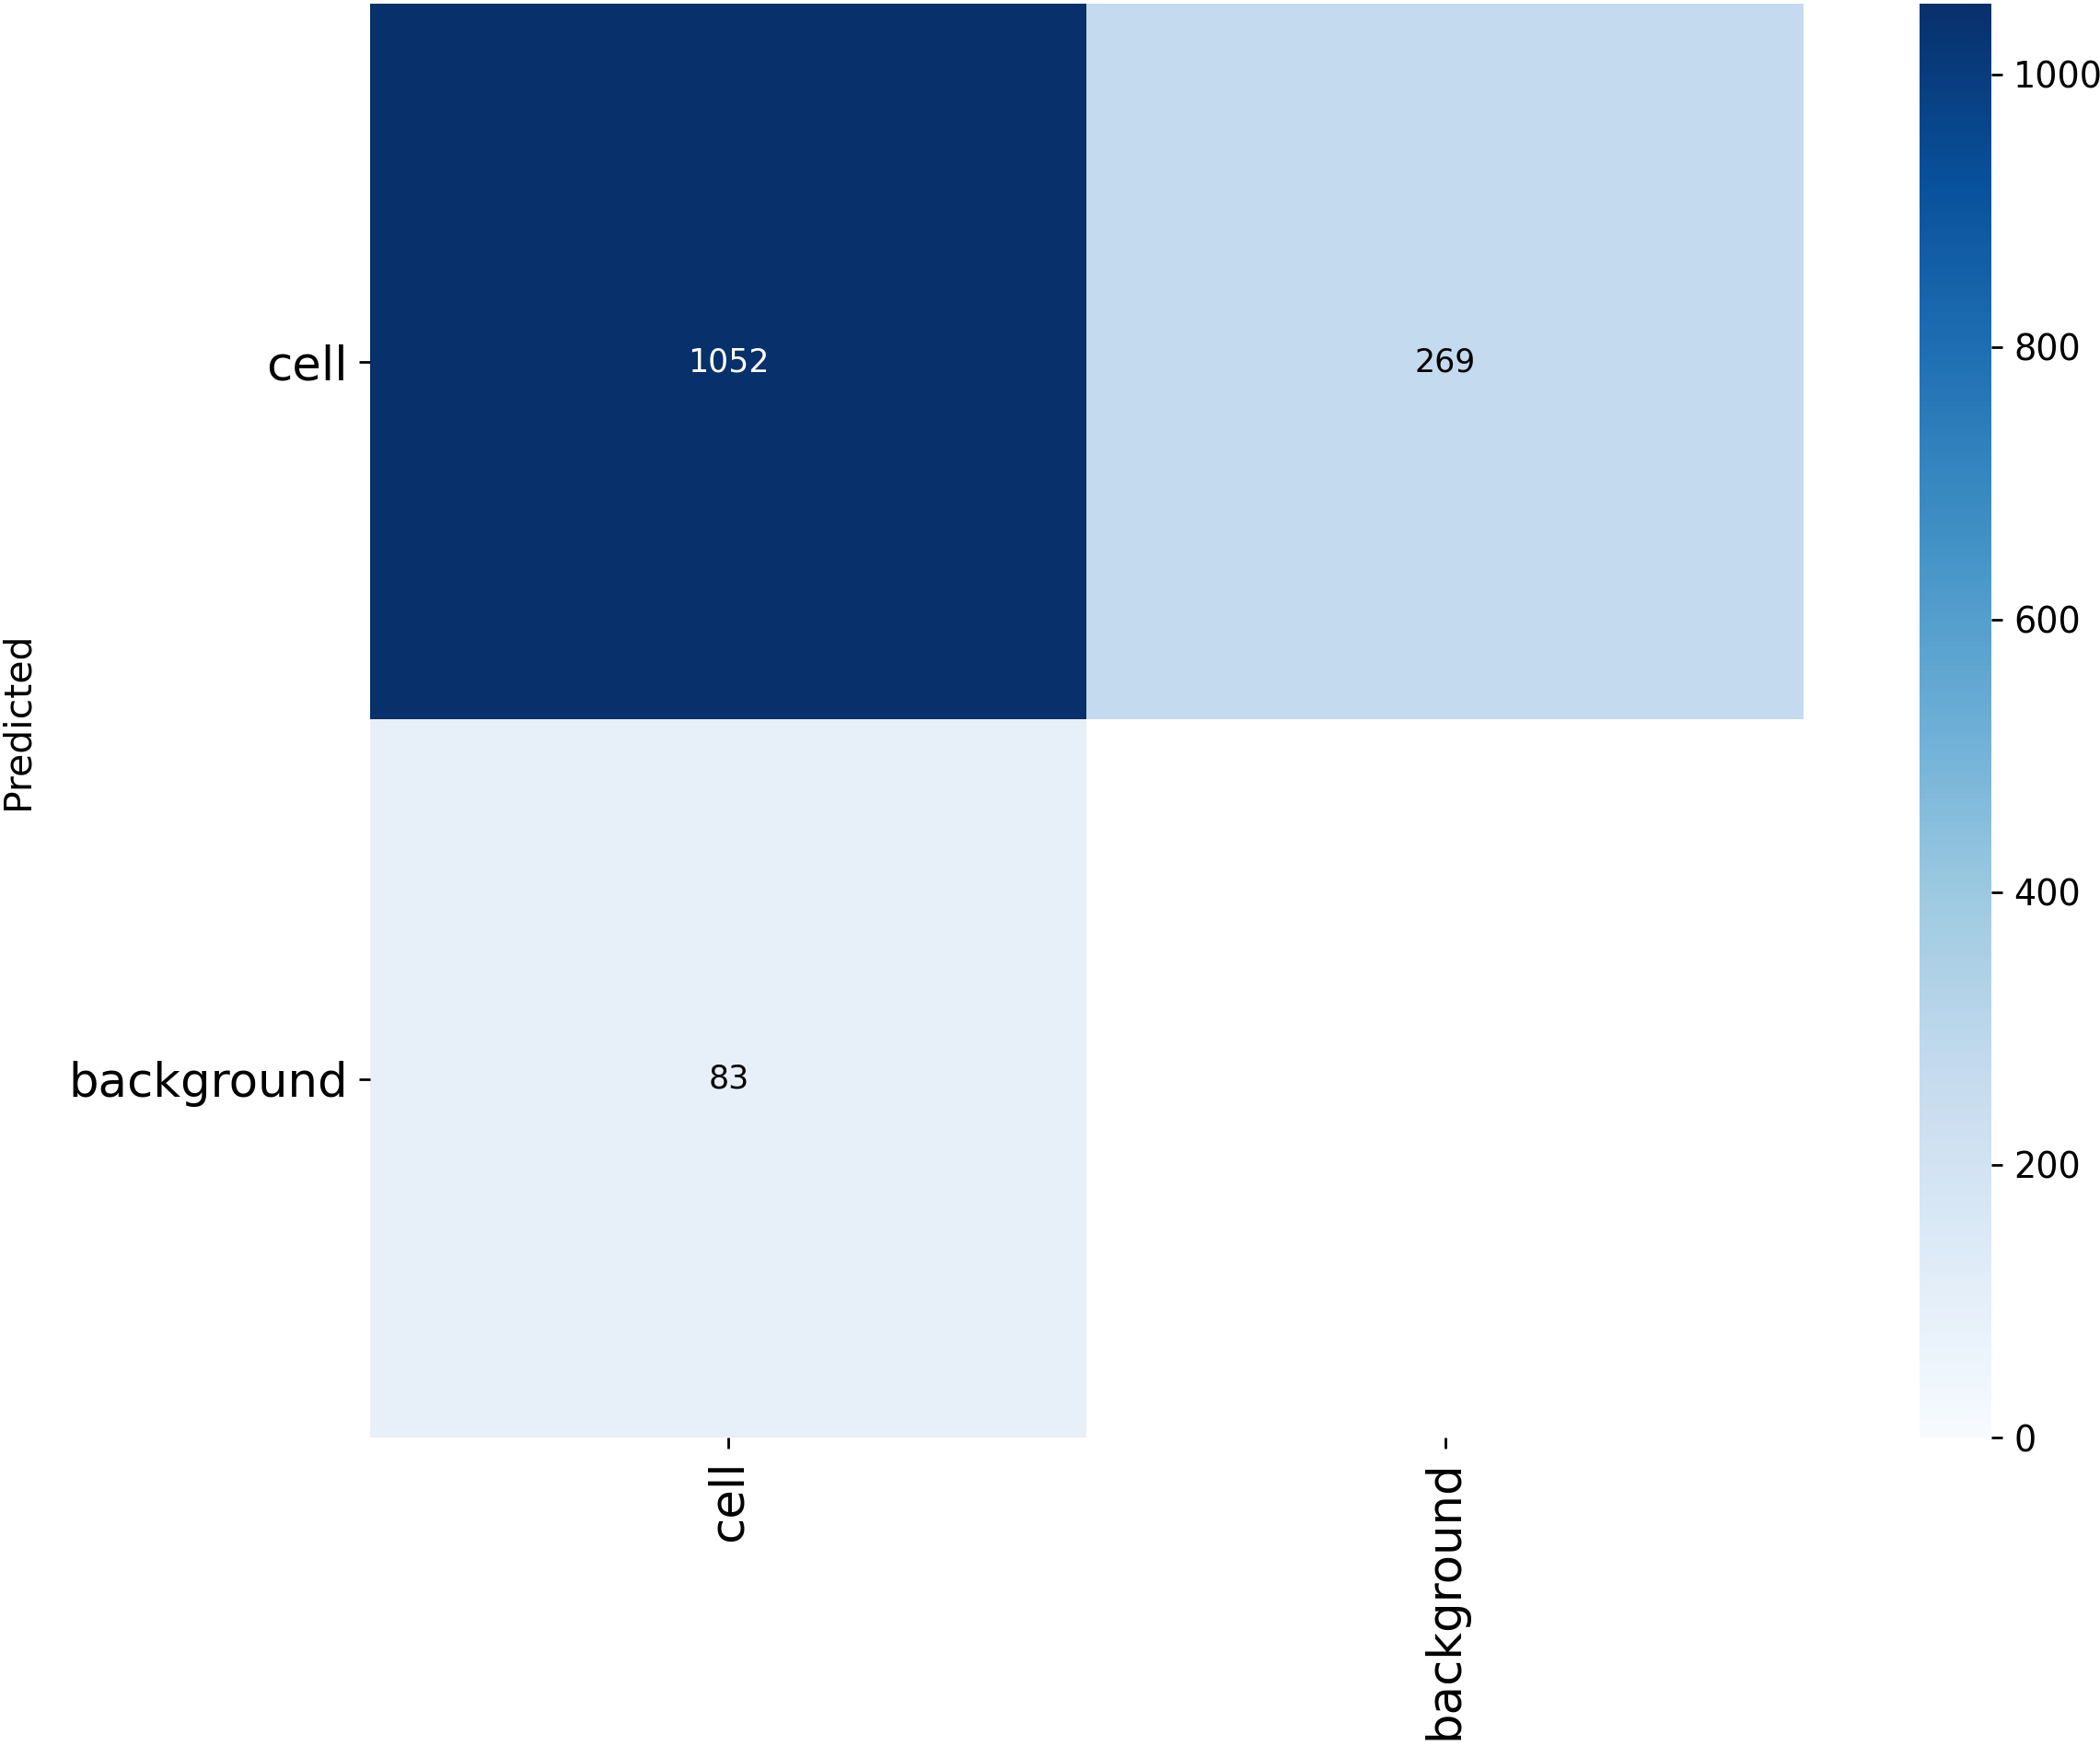
\includegraphics[height=5cm]{figuras/resultados experimentacion/yolov12l/test3/confusion_matrix.png}
    \vspace{-0.3cm}
    \caption{\footnotesize YOLOv12l}
    \label{fig:confusion_yolov12l_test3}
  \end{subfigure}
  
  \vspace{0.1cm}
  % Cuarta fila
  \begin{subfigure}[b]{0.45\textwidth}
    \centering
    \includegraphics[height=5cm]{figuras/resultados experimentacion/custom/test3/confusion_matrix.png}
    \vspace{-0.3cm}
    \caption{\footnotesize \textit{custom}}
    \label{fig:confusion_custom_test3}
  \end{subfigure}
  \hfill
  \begin{subfigure}[b]{0.45\textwidth}
    \centering
    \includegraphics[height=5cm]{figuras/resultados experimentacion/ensemble/confusion_matrices/confusion_matrix_test3.png}
    \vspace{-0.3cm}
    \caption{\footnotesize \textit{ensemble}}
    \label{fig:confusion_ensemble_test3}
  \end{subfigure}
  
  \vspace{-0.2cm}
  \caption{Matrices de confusión para los modelos evaluados en test3}
  \label{fig:confusion_matrices_test3}
\end{figure}

\section{Curvas F1-confianza}
\label{sec:Curvas F1-confianza}

% BLOQUE PARA ORIGINAL_TEST
\begin{figure}[H]
  \centering
  % Primera fila
  \captionsetup[subfigure]{skip=-0.03cm}
  \vspace{-0.6cm}
  \begin{subfigure}[b]{0.48\textwidth}
    \centering
    \includegraphics[width=\textwidth]{figuras/resultados experimentacion/yolov8s/original_test/BoxF1_curve.png}
    \caption{YOLOv8s}
    \label{fig:yolov8s_original_test}
  \end{subfigure}
  \hfill
  \begin{subfigure}[b]{0.48\textwidth}
    \centering
    \includegraphics[width=\textwidth]{figuras/resultados experimentacion/yolov9s/original_test/BoxF1_curve.png}
    \caption{YOLOv9s}
    \label{fig:yolov9s_original_test}
  \end{subfigure}
  
  \vspace{0.0cm}
  % Segunda fila
  \begin{subfigure}[b]{0.48\textwidth}
    \centering
    \includegraphics[width=\textwidth]{figuras/resultados experimentacion/yolov10s/original_test/BoxF1_curve.png}
    \caption{YOLOv10s}
    \label{fig:yolov10s_original_test}
  \end{subfigure}
  \hfill
  \begin{subfigure}[b]{0.48\textwidth}
    \centering
    \includegraphics[width=\textwidth]{figuras/resultados experimentacion/yolov11s/original_test/BoxF1_curve.png}
    \caption{YOLOv11s}
    \label{fig:yolov11s_original_test}
  \end{subfigure}
  
  \vspace{0.0cm}
  % Tercera fila
  \begin{subfigure}[b]{0.48\textwidth}
    \centering
    \includegraphics[width=\textwidth]{figuras/resultados experimentacion/yolov12s/original_test/BoxF1_curve.png}
    \caption{YOLOv12s}
    \label{fig:yolov12s_original_test}
  \end{subfigure}
  \hfill
  \begin{subfigure}[b]{0.48\textwidth}
    \centering
    \includegraphics[width=\textwidth]{figuras/resultados experimentacion/yolov12l/original_test/BoxF1_curve.png}
    \caption{YOLOv12l}
    \label{fig:yolov12l_original_test}
  \end{subfigure}
  
  \vspace{0.0cm}
  % Cuarta fila (solo 1 imagen)
  \begin{subfigure}[b]{0.48\textwidth}
    \centering
    \includegraphics[width=\textwidth]{figuras/resultados experimentacion/custom/original_test/BoxF1_curve.png}
    \caption{\textit{custom}}
    \label{fig:custom_original_test}
  \end{subfigure}
  
  \caption{Curvas F1-confianza para los modelos evaluados en original\_test}
  \label{fig:f1_curves_original_test}
\end{figure}


% BLOQUE PARA TEST
\begin{figure}[H]
  \centering
  % Primera fila
  \begin{subfigure}[b]{0.48\textwidth}
    \centering
    \includegraphics[width=\textwidth]{figuras/resultados experimentacion/yolov8s/test/BoxF1_curve.png}
    \caption{YOLOv8s}
    \label{fig:yolov8s_test}
  \end{subfigure}
  \hfill
  \begin{subfigure}[b]{0.48\textwidth}
    \centering
    \includegraphics[width=\textwidth]{figuras/resultados experimentacion/yolov9s/test/BoxF1_curve.png}
    \caption{YOLOv9s}
    \label{fig:yolov9s_test}
  \end{subfigure}
  
  \vspace{0.5cm}
  % Segunda fila
  \begin{subfigure}[b]{0.48\textwidth}
    \centering
    \includegraphics[width=\textwidth]{figuras/resultados experimentacion/yolov10s/test/BoxF1_curve.png}
    \caption{YOLOv10s}
    \label{fig:yolov10s_test}
  \end{subfigure}
  \hfill
  \begin{subfigure}[b]{0.48\textwidth}
    \centering
    \includegraphics[width=\textwidth]{figuras/resultados experimentacion/yolov11s/test/BoxF1_curve.png}
    \caption{YOLOv11s}
    \label{fig:yolov11s_test}
  \end{subfigure}
  
  \vspace{0.5cm}
  % Tercera fila
  \begin{subfigure}[b]{0.48\textwidth}
    \centering
    \includegraphics[width=\textwidth]{figuras/resultados experimentacion/yolov12s/test/BoxF1_curve.png}
    \caption{YOLOv12s}
    \label{fig:yolov12s_test}
  \end{subfigure}
  \hfill
  \begin{subfigure}[b]{0.48\textwidth}
    \centering
    \includegraphics[width=\textwidth]{figuras/resultados experimentacion/yolov12l/test/BoxF1_curve.png}
    \caption{YOLOv12l}
    \label{fig:yolov12l_test}
  \end{subfigure}
  
  \vspace{0.5cm}
  % Cuarta fila (solo 1 imagen)
  \begin{subfigure}[b]{0.48\textwidth}
    \centering
    \includegraphics[width=\textwidth]{figuras/resultados experimentacion/custom/test/BoxF1_curve.png}
    \caption{\textit{custom}}
    \label{fig:custom_test}
  \end{subfigure}
  
  \caption{Curvas F1-confianza para los modelos evaluados en test}
  \label{fig:f1_curves_test}
\end{figure}


% BLOQUE PARA TEST2
\begin{figure}[H]
  \centering
  % Primera fila
  \begin{subfigure}[b]{0.48\textwidth}
    \centering
    \includegraphics[width=\textwidth]{figuras/resultados experimentacion/yolov8s/test2/BoxF1_curve.png}
    \caption{YOLOv8s}
    \label{fig:yolov8s_test2}
  \end{subfigure}
  \hfill
  \begin{subfigure}[b]{0.48\textwidth}
    \centering
    \includegraphics[width=\textwidth]{figuras/resultados experimentacion/yolov9s/test2/BoxF1_curve.png}
    \caption{YOLOv9s}
    \label{fig:yolov9s_test2}
  \end{subfigure}
  
  \vspace{0.5cm}
  % Segunda fila
  \begin{subfigure}[b]{0.48\textwidth}
    \centering
    \includegraphics[width=\textwidth]{figuras/resultados experimentacion/yolov10s/test2/BoxF1_curve.png}
    \caption{YOLOv10s}
    \label{fig:yolov10s_test2}
  \end{subfigure}
  \hfill
  \begin{subfigure}[b]{0.48\textwidth}
    \centering
    \includegraphics[width=\textwidth]{figuras/resultados experimentacion/yolov11s/test2/BoxF1_curve.png}
    \caption{YOLOv11s}
    \label{fig:yolov11s_test2}
  \end{subfigure}
  
  \vspace{0.5cm}
  % Tercera fila
  \begin{subfigure}[b]{0.48\textwidth}
    \centering
    \includegraphics[width=\textwidth]{figuras/resultados experimentacion/yolov12s/test2/BoxF1_curve.png}
    \caption{YOLOv12s}
    \label{fig:yolov12s_test2}
  \end{subfigure}
  \hfill
  \begin{subfigure}[b]{0.48\textwidth}
    \centering
    \includegraphics[width=\textwidth]{figuras/resultados experimentacion/yolov12l/test2/BoxF1_curve.png}
    \caption{YOLOv12l}
    \label{fig:yolov12l_test2}
  \end{subfigure}
  
  \vspace{0.5cm}
  % Cuarta fila (solo 1 imagen)
  \begin{subfigure}[b]{0.48\textwidth}
    \centering
    \includegraphics[width=\textwidth]{figuras/resultados experimentacion/custom/test2/BoxF1_curve.png}
    \caption{\textit{custom}}
    \label{fig:custom_test2}
  \end{subfigure}
  
  \caption{Curvas F1-confianza para los modelos evaluados en test2}
  \label{fig:f1_curves_test2}
\end{figure}


% BLOQUE PARA TEST3
\begin{figure}[H]
  \centering
  % Primera fila
  \begin{subfigure}[b]{0.48\textwidth}
    \centering
    \includegraphics[width=\textwidth]{figuras/resultados experimentacion/yolov8s/test3/BoxF1_curve.png}
    \caption{YOLOv8s}
    \label{fig:yolov8s_test3}
  \end{subfigure}
  \hfill
  \begin{subfigure}[b]{0.48\textwidth}
    \centering
    \includegraphics[width=\textwidth]{figuras/resultados experimentacion/yolov9s/test3/BoxF1_curve.png}
    \caption{YOLOv9s}
    \label{fig:yolov9s_test3}
  \end{subfigure}
  
  \vspace{0.5cm}
  % Segunda fila
  \begin{subfigure}[b]{0.48\textwidth}
    \centering
    \includegraphics[width=\textwidth]{figuras/resultados experimentacion/yolov10s/test3/BoxF1_curve.png}
    \caption{YOLOv10s}
    \label{fig:yolov10s_test3}
  \end{subfigure}
  \hfill
  \begin{subfigure}[b]{0.48\textwidth}
    \centering
    \includegraphics[width=\textwidth]{figuras/resultados experimentacion/yolov11s/test3/BoxF1_curve.png}
    \caption{YOLOv11s}
    \label{fig:yolov11s_test3}
  \end{subfigure}
  
  \vspace{0.5cm}
  % Tercera fila
  \begin{subfigure}[b]{0.48\textwidth}
    \centering
    \includegraphics[width=\textwidth]{figuras/resultados experimentacion/yolov12s/test3/BoxF1_curve.png}
    \caption{YOLOv12s}
    \label{fig:yolov12s_test3}
  \end{subfigure}
  \hfill
  \begin{subfigure}[b]{0.48\textwidth}
    \centering
    \includegraphics[width=\textwidth]{figuras/resultados experimentacion/yolov12l/test3/BoxF1_curve.png}
    \caption{YOLOv12l}
    \label{fig:yolov12l_test3}
  \end{subfigure}
  
  \vspace{0.5cm}
  % Cuarta fila (solo 1 imagen)
  \begin{subfigure}[b]{0.48\textwidth}
    \centering
    \includegraphics[width=\textwidth]{figuras/resultados experimentacion/custom/test3/BoxF1_curve.png}
    \caption{\textit{custom}}
    \label{fig:custom_test3}
  \end{subfigure}
  
  \caption{Curvas F1-confianza para los modelos evaluados en test3}
  \label{fig:f1_curves_test3}
\end{figure}

\section{Resultados cualitativos}
\label{sec:Resultados cualitativos anexo}


\begin{figure}[H]
  \centering
  \begin{subfigure}[b]{0.48\textwidth}
    \centering
    \includegraphics[width=\textwidth]{figuras/evaluacion_cualitativa/7/7.jpg}
    \caption{Imagen evaluada por experto}
    \label{fig:exp_image_7}
  \end{subfigure}
  \hfill
  \begin{subfigure}[b]{0.48\textwidth}
    \centering
    \includegraphics[width=\textwidth]{figuras/evaluacion_cualitativa/7/7_v7.jpg}
    \caption{Prueba de concepto inicial}
    \label{fig:poc_image_7}
  \end{subfigure}
  
  \vspace{0.3cm} 
  
  \begin{subfigure}[b]{0.48\textwidth}
    \centering
    \includegraphics[width=\textwidth]{figuras/evaluacion_cualitativa/7/7_v12.jpg}
    \caption{Modelo YOLOv12s con IoU 0.5}
    \label{fig:yolov12s_IoU0.5_image_7}
  \end{subfigure}
  \hfill
  \begin{subfigure}[b]{0.48\textwidth}
    \centering
    \includegraphics[width=\textwidth]{figuras/evaluacion_cualitativa/7/7_ensemble.jpg}
    \caption{Modelo \textit{ensemble}}
    \label{fig:ensemble_image_7}
  \end{subfigure}

  \vspace{0.3cm}
  % Quinta subfigura centrada
  \begin{subfigure}[b]{0.48\textwidth}
    \centering
    \includegraphics[width=\textwidth]{figuras/evaluacion_cualitativa/7/7_v12_IoU0.25.jpg}
    \caption{Modelo YOLOv12s con IoU 0.25}
    \label{figyolov12s_IoU0.25_image_7}
  \end{subfigure}
  
  \caption{Resultados comparativos para la Figura 7}
  \label{fig:7}
\end{figure}


\begin{figure}[H]
  \centering
  \begin{subfigure}[b]{0.48\textwidth}
    \centering
    \includegraphics[width=\textwidth]{figuras/evaluacion_cualitativa/9/9.jpg}
    \caption{Imagen evaluada por experto}
    \label{fig:exp_image_9}
  \end{subfigure}
  \hfill
  \begin{subfigure}[b]{0.48\textwidth}
    \centering
    \includegraphics[width=\textwidth]{figuras/evaluacion_cualitativa/9/9_v7.jpg}
    \caption{Prueba de concepto inicial}
    \label{fig:poc_image_9}
  \end{subfigure}
  
  \vspace{0.3cm} 
  
  \begin{subfigure}[b]{0.48\textwidth}
    \centering
    \includegraphics[width=\textwidth]{figuras/evaluacion_cualitativa/9/9_v12.jpg}
    \caption{Modelo YOLOv12s con IoU 0.5}
    \label{fig:yolov12s_IoU0.5_image_9}
  \end{subfigure}
  \hfill
  \begin{subfigure}[b]{0.48\textwidth}
    \centering
    \includegraphics[width=\textwidth]{figuras/evaluacion_cualitativa/9/9_ensemble.jpg}
    \caption{Modelo \textit{ensemble}}
    \label{fig:ensemble_image_9}
  \end{subfigure}
  
  \vspace{0.3cm}
  % Quinta subfigura centrada
  \begin{subfigure}[b]{0.48\textwidth}
    \centering
    \includegraphics[width=\textwidth]{figuras/evaluacion_cualitativa/9/9_v12_IoU0.25.jpg}
    \caption{Modelo YOLOv12s con IoU 0.25}
    \label{figyolov12s_IoU0.25_image_9}
  \end{subfigure}

  \caption{Resultados comparativos para la Figura 9}
  \label{fig:9}
\end{figure}


\begin{figure}[H]
  \centering
  \begin{subfigure}[b]{0.48\textwidth}
    \centering
    \includegraphics[width=\textwidth]{figuras/evaluacion_cualitativa/38/38.jpg}
    \caption{Imagen evaluada por experto}
    \label{fig:exp_image_38}
  \end{subfigure}
  \hfill
  \begin{subfigure}[b]{0.48\textwidth}
    \centering
    \includegraphics[width=\textwidth]{figuras/evaluacion_cualitativa/38/38_v7.jpg}
    \caption{Prueba de concepto inicial}
    \label{fig:poc_image_38}
  \end{subfigure}
  
  \vspace{0.3cm} 
  
  \begin{subfigure}[b]{0.48\textwidth}
    \centering
    \includegraphics[width=\textwidth]{figuras/evaluacion_cualitativa/38/38_v12.jpg}
    \caption{Modelo YOLOv12s con IoU 0.5}
    \label{fig:yolov12s_IoU0.5_image_38}
  \end{subfigure}
  \hfill
  \begin{subfigure}[b]{0.48\textwidth}
    \centering
    \includegraphics[width=\textwidth]{figuras/evaluacion_cualitativa/38/38_ensemble.jpg}
    \caption{Modelo \textit{ensemble}}
    \label{fig:ensemble_image_38}
  \end{subfigure}

  \vspace{0.3cm}
  % Quinta subfigura centrada
  \begin{subfigure}[b]{0.48\textwidth}
    \centering
    \includegraphics[width=\textwidth]{figuras/evaluacion_cualitativa/38/38_v12_IoU0.25.jpg}
    \caption{Modelo YOLOv12s con IoU 0.25}
    \label{figyolov12s_IoU0.25_image_38}
  \end{subfigure}
  
  \caption{Resultados comparativos para la Figura 38}
  \label{fig:38}
\end{figure}


% Figura 95
\begin{figure}[H]
  \centering
  \begin{subfigure}[b]{0.48\textwidth}
    \centering
    \includegraphics[width=\textwidth]{figuras/evaluacion_cualitativa/95/95.jpg}
    \caption{Imagen evaluada por experto}
    \label{fig:exp_image_95}
  \end{subfigure}
  \hfill
  \begin{subfigure}[b]{0.48\textwidth}
    \centering
    \includegraphics[width=\textwidth]{figuras/evaluacion_cualitativa/95/95_v7.jpg}
    \caption{Prueba de concepto inicial}
    \label{fig:poc_image_95}
  \end{subfigure}
  
  \vspace{0.3cm} 
  
  \begin{subfigure}[b]{0.48\textwidth}
    \centering
    \includegraphics[width=\textwidth]{figuras/evaluacion_cualitativa/95/95_v12.jpg}
    \caption{Modelo YOLOv12s con IoU 0.5}
    \label{fig:yolov12s_IoU0.5_image_95}
  \end{subfigure}
  \hfill
  \begin{subfigure}[b]{0.48\textwidth}
    \centering
    \includegraphics[width=\textwidth]{figuras/evaluacion_cualitativa/95/95_ensemble.jpg}
    \caption{Modelo Ensemble}
    \label{fig:ensemble_image_95}
  \end{subfigure}

  \vspace{0.3cm}
  % Quinta subfigura centrada
  \begin{subfigure}[b]{0.48\textwidth}
    \centering
    \includegraphics[width=\textwidth]{figuras/evaluacion_cualitativa/95/95_v12_IoU0.25.jpg}
    \caption{Modelo YOLOv12s con IoU 0.25}
    \label{figyolov12s_IoU0.25_image_95}
  \end{subfigure}
  
  \caption{Resultados comparativos para la Figura 95}
  \label{fig:95}
\end{figure}

% Figura 139
\begin{figure}[H]
  \centering
  \begin{subfigure}[b]{0.48\textwidth}
    \centering
    \includegraphics[width=\textwidth]{figuras/evaluacion_cualitativa/139/139.jpg}
    \caption{Imagen evaluada por experto}
    \label{fig:exp_image_139}
  \end{subfigure}
  \hfill
  \begin{subfigure}[b]{0.48\textwidth}
    \centering
    \includegraphics[width=\textwidth]{figuras/evaluacion_cualitativa/139/139_v7.jpg}
    \caption{Prueba de concepto inicial}
    \label{fig:poc_image_139}
  \end{subfigure}
  
  \vspace{0.3cm} 
  
  \begin{subfigure}[b]{0.48\textwidth}
    \centering
    \includegraphics[width=\textwidth]{figuras/evaluacion_cualitativa/139/139_v12.jpg}
    \caption{Modelo YOLOv12s con IoU 0.5}
    \label{fig:yolov12s_IoU0.5_image_139}
  \end{subfigure}
  \hfill
  \begin{subfigure}[b]{0.48\textwidth}
    \centering
    \includegraphics[width=\textwidth]{figuras/evaluacion_cualitativa/139/139_ensemble.jpg}
    \caption{Modelo Ensemble}
    \label{fig:ensemble_image_139}
  \end{subfigure}

  \vspace{0.3cm}
  % Quinta subfigura centrada
  \begin{subfigure}[b]{0.48\textwidth}
    \centering
    \includegraphics[width=\textwidth]{figuras/evaluacion_cualitativa/139/139_v12_IoU0.25.jpg}
    \caption{Modelo YOLOv12s con IoU 0.25}
    \label{figyolov12s_IoU0.25_image_139}
  \end{subfigure}
  
  \caption{Resultados comparativos para la Figura 139}
  \label{fig:139}
\end{figure}

% Figura 142
\begin{figure}[H]
  \centering
  \begin{subfigure}[b]{0.48\textwidth}
    \centering
    \includegraphics[width=\textwidth]{figuras/evaluacion_cualitativa/142/142.jpg}
    \caption{Imagen evaluada por experto}
    \label{fig:exp_image_142}
  \end{subfigure}
  \hfill
  \begin{subfigure}[b]{0.48\textwidth}
    \centering
    \includegraphics[width=\textwidth]{figuras/evaluacion_cualitativa/142/142_v7.jpg}
    \caption{Prueba de concepto inicial}
    \label{fig:poc_image_142}
  \end{subfigure}
  
  \vspace{0.3cm} 
  
  \begin{subfigure}[b]{0.48\textwidth}
    \centering
    \includegraphics[width=\textwidth]{figuras/evaluacion_cualitativa/142/142_v12.jpg}
    \caption{Modelo YOLOv12s con IoU 0.5}
    \label{fig:yolov12s_IoU0.5_image_142}
  \end{subfigure}
  \hfill
  \begin{subfigure}[b]{0.48\textwidth}
    \centering
    \includegraphics[width=\textwidth]{figuras/evaluacion_cualitativa/142/142_ensemble.jpg}
    \caption{Modelo Ensemble}
    \label{fig:ensemble_image_142}
  \end{subfigure}
  
  \vspace{0.3cm}
  % Quinta subfigura centrada
  \begin{subfigure}[b]{0.48\textwidth}
    \centering
    \includegraphics[width=\textwidth]{figuras/evaluacion_cualitativa/142/142_v12_IoU0.25.jpg}
    \caption{Modelo YOLOv12s con IoU 0.25}
    \label{figyolov12s_IoU0.25_image_142}
  \end{subfigure}

  \caption{Resultados comparativos para la Figura 142}
  \label{fig:142}
\end{figure}

% Figura 221
\begin{figure}[H]
  \centering
  \begin{subfigure}[b]{0.48\textwidth}
    \centering
    \includegraphics[width=\textwidth]{figuras/evaluacion_cualitativa/221/221.jpg}
    \caption{Imagen evaluada por experto}
    \label{fig:exp_image_221}
  \end{subfigure}
  \hfill
  \begin{subfigure}[b]{0.48\textwidth}
    \centering
    \includegraphics[width=\textwidth]{figuras/evaluacion_cualitativa/221/221_v7.jpg}
    \caption{Prueba de concepto inicial}
    \label{fig:poc_image_221}
  \end{subfigure}
  
  \vspace{0.3cm} 
  
  \begin{subfigure}[b]{0.48\textwidth}
    \centering
    \includegraphics[width=\textwidth]{figuras/evaluacion_cualitativa/221/221_v12.jpg}
    \caption{Modelo YOLOv12s con IoU 0.5}
    \label{fig:yolov12s_IoU0.5_image_221}
  \end{subfigure}
  \hfill
  \begin{subfigure}[b]{0.48\textwidth}
    \centering
    \includegraphics[width=\textwidth]{figuras/evaluacion_cualitativa/221/221_ensemble.jpg}
    \caption{Modelo Ensemble}
    \label{fig:ensemble_image_221}
  \end{subfigure}

  \vspace{0.3cm}
  % Quinta subfigura centrada
  \begin{subfigure}[b]{0.48\textwidth}
    \centering
    \includegraphics[width=\textwidth]{figuras/evaluacion_cualitativa/221/221_v12_IoU0.25.jpg}
    \caption{Modelo YOLOv12s con IoU 0.25}
    \label{figyolov12s_IoU0.25_image_221}
  \end{subfigure}
  
  \caption{Resultados comparativos para la Figura 221}
  \label{fig:221}
\end{figure}

% Figura 347
\begin{figure}[H]
  \centering
  \begin{subfigure}[b]{0.48\textwidth}
    \centering
    \includegraphics[width=\textwidth]{figuras/evaluacion_cualitativa/347/347.jpg}
    \caption{Imagen evaluada por experto}
    \label{fig:exp_image_347}
  \end{subfigure}
  \hfill
  \begin{subfigure}[b]{0.48\textwidth}
    \centering
    \includegraphics[width=\textwidth]{figuras/evaluacion_cualitativa/347/347_v7.jpg}
    \caption{Prueba de concepto inicial}
    \label{fig:poc_image_347}
  \end{subfigure}
  
  \vspace{0.3cm} 
  
  \begin{subfigure}[b]{0.48\textwidth}
    \centering
    \includegraphics[width=\textwidth]{figuras/evaluacion_cualitativa/347/347_v12.jpg}
    \caption{Modelo YOLOv12s con IoU 0.5}
    \label{fig:yolov12s_IoU0.5_image_347}
  \end{subfigure}
  \hfill
  \begin{subfigure}[b]{0.48\textwidth}
    \centering
    \includegraphics[width=\textwidth]{figuras/evaluacion_cualitativa/347/347_ensemble.jpg}
    \caption{Modelo Ensemble}
    \label{fig:ensemble_image_347}
  \end{subfigure}

  \vspace{0.3cm}
  % Quinta subfigura centrada
  \begin{subfigure}[b]{0.48\textwidth}
    \centering
    \includegraphics[width=\textwidth]{figuras/evaluacion_cualitativa/347/347_v12_IoU0.25.jpg}
    \caption{Modelo YOLOv12s con IoU 0.25}
    \label{figyolov12s_IoU0.25_image_347}
  \end{subfigure}
  
  \caption{Resultados comparativos para la Figura 347}
  \label{fig:347}
\end{figure}

% Figura 415
\begin{figure}[H]
  \centering
  \begin{subfigure}[b]{0.48\textwidth}
    \centering
    \includegraphics[width=\textwidth]{figuras/evaluacion_cualitativa/415/415.jpg}
    \caption{Imagen evaluada por experto}
    \label{fig:exp_image_415}
  \end{subfigure}
  \hfill
  \begin{subfigure}[b]{0.48\textwidth}
    \centering
    \includegraphics[width=\textwidth]{figuras/evaluacion_cualitativa/415/415_v7.jpg}
    \caption{Prueba de concepto inicial}
    \label{fig:poc_image_415}
  \end{subfigure}
  
  \vspace{0.3cm} 
  
  \begin{subfigure}[b]{0.48\textwidth}
    \centering
    \includegraphics[width=\textwidth]{figuras/evaluacion_cualitativa/415/415_v12.jpg}
    \caption{Modelo YOLOv12s con IoU 0.5}
    \label{fig:yolov12s_IoU0.5_image_415}
  \end{subfigure}
  \hfill
  \begin{subfigure}[b]{0.48\textwidth}
    \centering
    \includegraphics[width=\textwidth]{figuras/evaluacion_cualitativa/415/415_ensemble.jpg}
    \caption{Modelo Ensemble}
    \label{fig:ensemble_image_415}
  \end{subfigure}

  \vspace{0.3cm}
  % Quinta subfigura centrada
  \begin{subfigure}[b]{0.48\textwidth}
    \centering
    \includegraphics[width=\textwidth]{figuras/evaluacion_cualitativa/415/415_v12_IoU0.25.jpg}
    \caption{Modelo YOLOv12s con IoU 0.25}
    \label{figyolov12s_IoU0.25_image_415}
  \end{subfigure}
  
  \caption{Resultados comparativos para la Figura 415}
  \label{fig:415}
\end{figure}

% Figura 461
\begin{figure}[H]
  \centering
  \begin{subfigure}[b]{0.48\textwidth}
    \centering
    \includegraphics[width=\textwidth]{figuras/evaluacion_cualitativa/461/461.jpg}
    \caption{Imagen evaluada por experto}
    \label{fig:exp_image_461}
  \end{subfigure}
  \hfill
  \begin{subfigure}[b]{0.48\textwidth}
    \centering
    \includegraphics[width=\textwidth]{figuras/evaluacion_cualitativa/461/461_v7.jpg}
    \caption{Prueba de concepto inicial}
    \label{fig:poc_image_461}
  \end{subfigure}
  
  \vspace{0.3cm} 
  
  \begin{subfigure}[b]{0.48\textwidth}
    \centering
    \includegraphics[width=\textwidth]{figuras/evaluacion_cualitativa/461/461_v12.jpg}
    \caption{Modelo YOLOv12s con IoU 0.5}
    \label{fig:yolov12s_IoU0.5_image_461}
  \end{subfigure}
  \hfill
  \begin{subfigure}[b]{0.48\textwidth}
    \centering
    \includegraphics[width=\textwidth]{figuras/evaluacion_cualitativa/461/461_ensemble.jpg}
    \caption{Modelo Ensemble}
    \label{fig:ensemble_image_461}
  \end{subfigure}

  \vspace{0.3cm}
  % Quinta subfigura centrada
  \begin{subfigure}[b]{0.48\textwidth}
    \centering
    \includegraphics[width=\textwidth]{figuras/evaluacion_cualitativa/461/461_v12_IoU0.25.jpg}
    \caption{Modelo YOLOv12s con IoU 0.25}
    \label{figyolov12s_IoU0.25_image_461}
  \end{subfigure}
  
  \caption{Resultados comparativos para la Figura 461}
  \label{fig:461}
\end{figure}


\end{document}


% % % Cambio de nombre del TFM
% % ¿cuando sabemos fecha y tribunal?